% ******************************* PhD Thesis Template **************************
% Please have a look at the README.md file for info on how to use the template

\documentclass[a4paper,12pt,times,numbered,print,index]{Classes/PhDThesisPSnPDF}

% ******************************************************************************
% ******************************* Class Options ********************************
% *********************** See README for more details **************************
% ******************************************************************************

% `a4paper'(The University of Cambridge PhD thesis guidelines recommends a page
% size a4 - default option) or `a5paper': A5 Paper size is also allowed as per
% the Cambridge University Engineering Deparment guidelines for PhD thesis
%
% `11pt' or `12pt'(default): Font Size 10pt is NOT recommended by the University
% guidelines
%
% `oneside' or `twoside'(default): Printing double side (twoside) or single
% side.
%
% `print': Use `print' for print version with appropriate margins and page
% layout. Leaving the options field blank will activate Online version.
%
% `index': For index at the end of the thesis
%
% `draftclassic': For draft mode without loading any images (same as draft in book)
%
% `draft': Special draft mode with line numbers, images, and water mark with
% timestamp and custom text. Position of the text can also be modified.
%
% `abstract': To generate only the title page and abstract page with
% dissertation title and name, to submit to the Student Registry
%
% `chapter`: This option enables only the specified chapter and it's references
%  Useful for review and corrections.
%
% ************************* Custom Page Margins ********************************
%
% `custommargin`: Use `custommargin' in options to activate custom page margins,
% which can be defined in the preamble.tex. Custom margin will override
% print/online margin setup.
%
% *********************** Choosing the Fonts in Class Options ******************
%
% `times' : Times font with math support. (The Cambridge University guidelines
% recommend using times)
%
% `fourier': Utopia Font with Fourier Math font (Font has to be installed)
%            It's a free font.
%
% `customfont': Use `customfont' option in the document class and load the
% package in the preamble.tex
%
% default or leave empty: `Latin Modern' font will be loaded.
%
% ********************** Choosing the Bibliography style ***********************
%
% `authoryear': For author-year citation eg., Krishna (2013)
%
% `numbered': (Default Option) For numbered and sorted citation e.g., [1,5,2]
%
% `custombib': Define your own bibliography style in the `preamble.tex' file.
%              `\RequirePackage[square, sort, numbers, authoryear]{natbib}'.
%              This can be also used to load biblatex instead of natbib
%              (See Preamble)
%
% **************************** Choosing the Page Style *************************
%
% `default (leave empty)': For Page Numbers in Header (Left Even, Right Odd) and
% Chapter Name in Header (Right Even) and Section Name (Left Odd). Blank Footer.
%
% `PageStyleI': Chapter Name next & Page Number on Even Side (Left Even).
% Section Name & Page Number in Header on Odd Side (Right Odd). Footer is empty.
%
% `PageStyleII': Chapter Name on Even Side (Left Even) in Header. Section Number
% and Section Name in Header on Odd Side (Right Odd). Page numbering in footer

% Uncomment to change page style
%\pagestyle{PageStyleII}

% ********************************** Preamble **********************************
% Preamble: Contains packages and user-defined commands and settings
% ******************************************************************************
% ****************************** Custom Margin *********************************

% Add `custommargin' in the document class options to use this section
% Set {innerside margin / outerside margin / topmargin / bottom margin}  and
% other page dimensions
\ifsetCustomMargin
  \RequirePackage[left=37mm,right=30mm,top=35mm,bottom=30mm]{geometry}
  \setFancyHdr % To apply fancy header after geometry package is loaded
\fi

% Add spaces between paragraphs
%\setlength{\parskip}{0.5em}
% Ragged bottom avoids extra whitespaces between paragraphs
\raggedbottom
% To remove the excess top spacing for enumeration, list and description
%\usepackage{enumitem}
%\setlist[enumerate,itemize,description]{topsep=0em}

% *****************************************************************************
% ******************* Fonts (like different typewriter fonts etc.)*************

% Add `customfont' in the document class option to use this section

\ifsetCustomFont
  % Set your custom font here and use `customfont' in options. Leave empty to
  % load computer modern font (default LaTeX font).
  %\RequirePackage{helvet}

  % For use with XeLaTeX
  %  \setmainfont[
  %    Path              = ./libertine/opentype/,
  %    Extension         = .otf,
  %    UprightFont = LinLibertine_R,
  %    BoldFont = LinLibertine_RZ, % Linux Libertine O Regular Semibold
  %    ItalicFont = LinLibertine_RI,
  %    BoldItalicFont = LinLibertine_RZI, % Linux Libertine O Regular Semibold Italic
  %  ]
  %  {libertine}
  %  % load font from system font
  %  \newfontfamily\libertinesystemfont{Linux Libertine O}
\fi

% *****************************************************************************
% **************************** Custom Packages ********************************

% ************************* Algorithms and Pseudocode **************************

%\usepackage{algpseudocode}


% ********************Captions and Hyperreferencing / URL **********************

% Captions: This makes captions of figures use a boldfaced small font.
%\RequirePackage[small,bf]{caption}

\RequirePackage[labelsep=space,tableposition=top]{caption}
\renewcommand{\figurename}{Fig.} %to support older versions of captions.sty


% *************************** Graphics and figures *****************************

%\usepackage{rotating}
%\usepackage{wrapfig}

% Uncomment the following two lines to force Latex to place the figure.
% Use [H] when including graphics. Note 'H' instead of 'h'
%\usepackage{float}
%\restylefloat{figure}

% Subcaption package is also available in the sty folder you can use that by
% uncommenting the following line
% This is for people stuck with older versions of texlive
%\usepackage{sty/caption/subcaption}
\usepackage{subcaption}

% ********************************** Tables ************************************
\usepackage{booktabs} % For professional looking tables
\usepackage{multirow}

%\usepackage{multicol}
%\usepackage{longtable}
%\usepackage{tabularx}


% *********************************** SI Units *********************************
\usepackage{siunitx} % use this package module for SI units


% ******************************* Line Spacing *********************************

% Choose linespacing as appropriate. Default is one-half line spacing as per the
% University guidelines

% \doublespacing
% \onehalfspacing
% \singlespacing


% ************************ Formatting / Footnote *******************************

% Don't break enumeration (etc.) across pages in an ugly manner (default 10000)
%\clubpenalty=500
%\widowpenalty=500

%\usepackage[perpage]{footmisc} %Range of footnote options


% *****************************************************************************
% *************************** Bibliography  and References ********************

%\usepackage{cleveref} %Referencing without need to explicitly state fig /table

% Add `custombib' in the document class option to use this section
\ifuseCustomBib
   \RequirePackage[square, sort, numbers, authoryear]{natbib} % CustomBib

% If you would like to use biblatex for your reference management, as opposed to the default `natbibpackage` pass the option `custombib` in the document class. Comment out the previous line to make sure you don't load the natbib package. Uncomment the following lines and specify the location of references.bib file

%\RequirePackage[backend=biber, style=numeric-comp, citestyle=numeric, sorting=nty, natbib=true]{biblatex}
%\bibliography{References/references} %Location of references.bib only for biblatex

\fi

% changes the default name `Bibliography` -> `References'
\renewcommand{\bibname}{References}


% ******************************************************************************
% ************************* User Defined Commands ******************************
% ******************************************************************************

% *********** To change the name of Table of Contents / LOF and LOT ************

%\renewcommand{\contentsname}{My Table of Contents}
%\renewcommand{\listfigurename}{My List of Figures}
%\renewcommand{\listtablename}{My List of Tables}


% ********************** TOC depth and numbering depth *************************

\setcounter{secnumdepth}{3}
\setcounter{tocdepth}{2}


% ******************************* Nomenclature *********************************

% To change the name of the Nomenclature section, uncomment the following line

%\renewcommand{\nomname}{Symbols}


% ********************************* Appendix ***********************************

% The default value of both \appendixtocname and \appendixpagename is `Appendices'. These names can all be changed via:

%\renewcommand{\appendixtocname}{List of appendices}
%\renewcommand{\appendixname}{Appndx}

% *********************** Configure Draft Mode **********************************

% Uncomment to disable figures in `draft'
%\setkeys{Gin}{draft=true}  % set draft to false to enable figures in `draft'

% These options are active only during the draft mode
% Default text is "Draft"
%\SetDraftText{DRAFT}

% Default Watermark location is top. Location (top/bottom)
%\SetDraftWMPosition{bottom}

% Draft Version - default is v1.0
%\SetDraftVersion{v1.1}

% Draft Text grayscale value (should be between 0-black and 1-white)
% Default value is 0.75
%\SetDraftGrayScale{0.8}


% ******************************** Todo Notes **********************************
%% Uncomment the following lines to have todonotes.

%\ifsetDraft
%	\usepackage[colorinlistoftodos]{todonotes}
%	\newcommand{\mynote}[1]{\todo[author=kks32,size=\small,inline,color=green!40]{#1}}
%\else
%	\newcommand{\mynote}[1]{}
%	\newcommand{\listoftodos}{}
%\fi

% Example todo: \mynote{Hey! I have a note}

% ************************ Thesis Information & Meta-data **********************
% Thesis title and author information, refernce file for biblatex
% ************************ Thesis Information & Meta-data **********************
%% The title of the thesis
\title{Memristive Silicon Oxide Devices for Biorealistic Learning}
%\texorpdfstring is used for PDF metadata. Usage:
%\texorpdfstring{LaTeX_Version}{PDF Version (non-latex)} eg.,
%\texorpdfstring{$sigma$}{sigma}

%% Subtitle (Optional)
% \subtitle{Transfer Report}

%% The full name of the author
\author{Viet Cuong Vu}

%% Department (eg. Department of Engineering, Maths, Physics)
\dept{Faculty of Engineering Sciences}


%% University and Crest
\university{University College London}
% Crest minimum should be 30mm.
\crest{
\includegraphics[width=0.75\textwidth]{Figs/ucl-logo-black-on-grey.jpg}}
%% Use this crest, if you are using the college crest
%% Crest long miminum should be 65mm
%\crest{
\includegraphics[width=0.45\textwidth]{University_Crest_Long}}

%% College shield [optional] 
% Crest minimum should be 30mm.
%\collegeshield{
\includegraphics[width=0.2\textwidth]{CollegeShields/Kings}}


%% Supervisor (optional)
%% for multiple supervisors, append each supervisor with the \newline command
\supervisor{\normalsize{Principal Supervisor: Anthony J. Kenyon \newline Subsidiary Supervisor: Adnan Mehonic}}
%% Supervisor Role (optional) - Supervisor (default) or advisor
\supervisorrole{}
%% if no title is desired:
% \supervisorrole{}
%% Supervisor line width: required to align supervisors
\supervisorlinewidth{0.45\textwidth}


%% Advisor (optional)
%% for multiple advisors, append each advisor with the \newline command
% \advisor{\normalsize{Adnan Mehonic}}    
%% Advisor Role (optional) - Advisor (default) or leave empty
% \advisorrole{\normalsize{Subsidiary Supervisor: }}
%% if no title is required
% \advisorrole{}
%% Advisor line width: required to align supervisors
% \advisorlinewidth{0.27\textwidth}


%% You can redefine the submission text:
% Default as per the University guidelines:
% ``This dissertation is submitted for the degree of''
\renewcommand{\submissiontext}{This dissertation is submitted in partial fulfilment for the degree of}

%% Full title of the Degree
\degreetitle{Doctor of Philosophy}

%% College affiliation (optional)
% \college{Robinson's College}

%% Submission date
% Default is set as {\monthname[\the\month]\space\the\year}
%\degreedate{September 2014} 

%% Meta information
\subject{LaTeX} \keywords{{LaTeX} {PhD Thesis} {Engineering Science} {University College London}}


% ***************************** Abstract Separate ******************************
% To printout only the titlepage and the abstract with the PhD title and the
% author name for submission to the Student Registry, use the `abstract' option in
% the document class.

\ifdefineAbstract
 \pagestyle{empty}
 \includeonly{Declaration/declaration, Abstract/abstract}
\fi

% ***************************** Chapter Mode ***********************************
% The chapter mode allows user to only print particular chapters with references
% Title, Contents, Frontmatter are disabled by default
% Useful option to review a particular chapter or to send it to supervisior.
% To use choose `chapter' option in the document class

\ifdefineChapter
 \includeonly{Chapter3/chapter3}
\fi

% ******************************** Front Matter ********************************
\begin{document}

\frontmatter

\maketitle

% % ******************************* Thesis Dedidcation ********************************

\begin{dedication} 

I would like to dedicate this thesis to my loving parents \dots

\end{dedication}
% ******************************* Thesis Declaration ***************************

\begin{declaration}

    I, Viet Cuong Vu, confirm that the work presented in this thesis is my own. 
    Where information has been derived from other sources, I confirm that this has been indicated in the thesis.  

% Author and date will be inserted automatically from thesis.tex \author \degreedate

\end{declaration}
% ************************** Thesis Abstract *****************************
% Use `abstract' as an option in the document class to print only the titlepage and the abstract.
\begin{abstract}

\noindent This thesis presents a comprehensive exploration of biorealistic learning on memristive networks, offering a layered approach that bridges device-level physics and system-level neuromorphic computation. Beginning with a neuroscience primer to ground the discussion in biological plausibility, the chapters systematically progresses through the physics of memristive devices, highlighting their nonlinear dynamics, memory retention mechanisms, and analog switching behaviors. Particular attention is paid to how these physical properties underpin essential computational primitives such as spike-timing-dependent plasticity (STDP), long-term potentiation/depression, and homeostatic regulation.\\

\noindent Through analytical modeling and circuit-level abstraction, the work demonstrates how the intrinsic dynamics of memristors—such as voltage-controlled conductance modulation and ionic drift—map naturally onto biologically inspired learning rules. By anchoring the investigation in real-world material characteristics, such as variability, non-volatility, and resistive switching kinetics, this provides a foundation for designing spiking neural networks (SNNs) that are not only computationally efficient but also physically grounded in the behavior of nanoscale hardware.\\

\noindent This device-to-algorithm pipeline allows for a more faithful reproduction of synaptic processes in silicon, paving the way for energy-efficient, adaptive, and scalable neuromorphic systems. Ultimately, the research argues that an informed understanding of device physics is not peripheral but central to developing biorealistic SNN architectures that can emulate the functional and learning capabilities of biological systems.


\end{abstract}

% ************************** Thesis Impact Statement **************************

\begin{impact}      

\noindent This thesis advances the frontier of neuromorphic engineering by presenting a comprehensive, multi-scale investigation into biorealistic learning on memristive networks, bridging device physics, circuit modeling, and system integration. The research offers a sequential and coherent progression of contributions, addressing multiple critical layers of abstraction, arriving at novel artificial intelligence architectures grounded in physical memristive behavior. \\

\noindent At the device level, the thesis begins with the experimental characterization of silicon oxide memristors in the subthreshold regime, revealing their potential for unipolar potentiation and depression—a key mechanism for mimicking biological synaptic plasticity. This was published in IEEE NANO 2023 and presented at EMRS 2025, establishing foundational insights into the neuromorphic viability of subthreshold device operation. \\

\noindent Building on this, the circuit-level work involved the development of SPICE-compatible compact models that accurately capture transient behaviors within subthreshold memristors. Presented at MetroXRAINE 2023 and MEMRISYS 2024, these models enable scalable circuit simulations and lay the groundwork for integrating the current transient under subthreshold device operation into higher-level architectures. \\

\noindent At the system level, the thesis culminates in the implementation of spiking neural networks trained on hardware-aware, biorealistic learning rules. Presented at IEEE NANO 2024 and SEAI 2025 where it was awarded a conference prize for best presentation, then published in their respective proceedings, these architectures demonstrate robust performance while integrating synaptic learning with physics informed constraints. \\

\noindent The thesis thus delivers a vertically integrated exploration—from material behavior to functional cognition—demonstrating the viability of memristive silicon oxide devices for brain-inspired computing. This provides not only theoretical and experimental tools, but also a blueprint for future hardware implementations of biorealistic artificial intelligence systems.\\

\clearpage
\thispagestyle{empty}
\section*{\centering Contributions}

\subsection*{List of Publications}
\begin{itemize}
    \item V. C. Vu, D. J. Mannion, D. Joksas, W. H. Ng, A. Mehonic, and A. Kenyon, “Spiking Neural Networks with Silicon Oxide Memristive Devices in the Subthreshold Regime,” in 2025 IEEE 5th International Conference on Software Engineering and Artificial Intelligence, Jul. 2025, pp. 340–344.
    \item V. C. Vu, A. Kenyon, D. Joksas, A. Mehonic, D. J. Mannion, and W. H. Ng, “Spiking Neural Networks with Nonidealities from Memristive Silicon Oxide Devices,” in 2024 IEEE 24th International Conference on Nanotechnology, Jul. 2024, pp. 46–50.
    \item D. J. Mannion, V. C. Vu, W. H. Ng, A. Mehonic, and A. J. Kenyon, “Unipolar Potentiation and Depression in Memristive Devices Utilizing the Subthreshold Regime,” IEEE Transactions on Nanotechnology, vol. 22, pp. 313–320, 2023.
\end{itemize}

\subsection*{Conference Presentations}

\begin{itemize}
    \item "Unipolar Potentiation and Depression within Optically Active Memristive Devices Subthreshold Regime", EMRS Spring 2025.
    \item "Circuit-Based Modelling of Current Transients within the Memristive Devices Subthreshold Regime", MEMRISYS 2024.
    \item "A Compact SPICE Model for Current Transients within the Subthreshold Regime of Memristors", IEEE MetroXRAINE 2023.
  \end{itemize}

\end{impact}

% ************************** Thesis Acknowledgements **************************

\begin{acknowledgements}      

\noindent latex.
\\

\end{acknowledgements}



% *********************** Adding TOC and List of Figures ***********************

\tableofcontents

\listoffigures

\listoftables

% \printnomenclature[space] space can be set as 2em between symbol and description
%\printnomenclature[3em]

% \printnomenclature

% ******************************** Main Matter *********************************
\mainmatter

%!TEX root = ../thesis.tex
%*******************************************************************************
%*********************************** First Chapter *****************************
%*******************************************************************************

\chapter{Introduction}  %Title of the First Chapter


\section[Background]{Background}

Neuromorphic computing aims to bridge the gap between neuroscience and artificial intelligence by emulating the structural and functional principles of biological neural systems. At the heart of this vision is a pressing research question: how can we implement biorealistic learning on memristive networks to develop energy-efficient, scalable and adaptive computing architectures? Addressing this question requires a multidisciplinary approach, combining insights from neurobiology, electronic materials science and computational modelling. \\

\noindent Traditional von Neumann architectures \cite{von1993first}, characterised by their separation of memory and processing units, struggle to efficiently handle tasks that the human brain performs effortlessly, such as pattern recognition, sensory integration, and decision making. In contrast, the brain achieves these feats with remarkable energy efficiency and adaptability, in part due to the tightly coupled nature of computation and memory in its neural circuits. Mimicking these biological characteristics in silicon and emerging nanotechnologies has become the guiding principle of neuromorphic engineering \cite{saighi2015plasticity}. \\

\noindent Recent advances in memristive technologies have reignited interest in neuromorphic computing. Memristors, or memory resistors, are two-terminal non-volatile devices that can emulate synaptic plasticity by adjusting their conductance based on the history of voltage and current applied. This property lend itself to naturally support learning rules such as Hebbian learning \cite{hebb2005organization} and spike-timing-dependent plasticity (STDP) \cite{markram1997regulation}. When arranged in crossbar arrays, memristors offer a promising platform for in-memory computation, which can significantly reduce the power and latency associated with traditional data transfer bottlenecks. \\

\noindent This chapter presents a comprehensive discussion of biorealistic learning mechanisms and their physical realisation on memristive networks. By grounding the discussion in the neuroscientific principles that underlie learning and cognition, the chapter aims to elucidate how these biological processes can be abstracted and implemented in hardware. \\

\noindent The chapter begins with an overview of the biological basis of computation, providing an essential neuroscience primer. It then moves to device-level considerations, discussing the properties of memristive devices and their integration into neuromorphic architectures. Throughout, the emphasis is on aligning computational models with biological fidelity, while navigating the constraints and opportunities offered by emerging nanotechnologies.

\section[Neuroscience Primers]{Neuroscience Primers}

Computational neuroscience employs a computational methodology to elucidate the mechanisms underlying brain function. This entails not only identifying the computations performed by the brain but also understanding the interactions between brain elements, such as neurons and synapses, that facilitate these computations.\\

% \noindent The field of computational neuroscience has traditionally adopted a bottom-up approach, commencing with the study of individual neurons and subsequently examining how these can be integrated into progressively larger networks, ultimately leading to the emergence of meaningful behaviour. \\

% \noindent In contrast, psychology and cognitive science have adopted a more top-down approach, commencing with the observation of animal behaviour and subsequently attempting to elucidate the brain mechanisms underlying these behaviours in terms of the higher-level functions of large brain areas. \\

% \noindent This distinction has resulted in a historical focus on developing comprehensive mathematical models of individual neurons and small- to medium-sized networks in computational neuroscience. Recently, however, there has been a convergence with other fields, leading to the creation of neurally detailed models capable of reproducing organism-level behaviors. \\

\noindent This section provides foundational relevant biological details, both at the neural level and at the network level. It should be noted that the models detailed in this dissertaion are still relatively basic in comparison to the extensive body of evidence documenting the neural system \cite{kandel2000principles} which provide the majority of our neural data about these areas. Consequently, this section presents only the most fundamental biological facts relevant to this work.

\subsection[Neuron Anatomy and Electrophysiology]{Neuron Anatomy and Electrophysiology}

\noindent  A neuron is a specialised biological cell that processes and transmits information through electrical and chemical signals \cite{mel1994information}. They represent only one of the numerous cell types within the brain, yet they are the most frequently discussed due to their status as the primary computational entities. Their fundamental function is relatively straightforward: neurons receive input from other neurons, and if that input is sufficiently stimulating, they will fire an action potential (also known as a spike), which propagates to other neurons.\\

\noindent Figure \ref{fig:1a} illustrates the basic structure of a neuron. Neurons can be subdivided into three principal parts: the dendrites, the cell body (soma), and the axon. Neurons receive input currents via their dendrites, which then transmit or channel this into the cell body, called the soma. When a neuron spikes, it sends current down its axon, which results in the release of neurotransmitter(s) at the synapses. These are connections from a neuron's axon to the dendrites of other neurons, and the neurotransmitter release causes dendritic input currents in these other connected neurons. \\

\begin{figure}[htbp!] 
    \centering    
    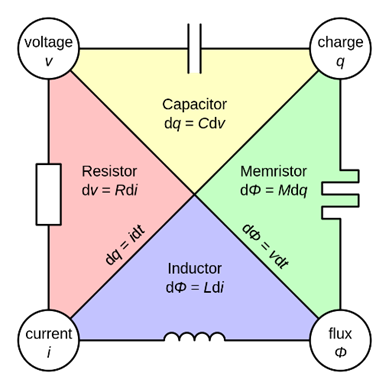
\includegraphics[width=0.5\textwidth]{Chapter1/Figs/1a.png}
    \caption[Labeled diagram of the neuron.]{Labeled diagram of the neuron, nerve cell that is the main part of the nervous system. A neuron's dendrites include synapses that allow it to accept input from other neurons. The dendrites carry current to the soma, which is where electrical charge is integrated. If the neuron membrane gets sufficiently polarised, an action potential (also known as a spike) travels down the axon. This causes neurotransmitters to be released at synapses, resulting in currents in the dendrites of postsynaptic neurons.}
    \label{fig:1a}
    \end{figure}

\noindent From a computational perspective, the soma represents the integration point for all incoming currents from dendrites \cite{polsky2004computational}, marking the initiation of the action potential generation process (Figure \ref{fig:1b}). When a neuron is at rest, the soma exhibits a negative charge. This is referred to as the resting voltage and is maintained by ion pumps that regulate the concentration of ions (predominantly sodium, $Na^+$, potassium, $K^+$, and calcium, $Ca^{+2}$) within the cell. \\


\noindent As the currents arrive from the dendrites, they initiate a process of depolarisation of the cell \cite{johnston1996active}. Once the voltage within the soma reaches a sufficient level, it initiates the opening of voltage-activated sodium channels, which permit the influx of sodium ions into the cell, further depolarising it. This process persists until the electrical gradient resulting from the accumulation of sodium ions reaches a point where it is no longer in equilibrium with the chemical gradient caused by the imbalance of sodium within and outside the cell. This leads to a notable increase in the neuron's positive charge, exceeding the resting voltage. \\

\noindent Furthermore, this substantial depolarisation also activates voltage-gated potassium channels, which subsequently permit the release of potassium ions from the cell, thereby facilitating repolarisation. Concurrently, the sodium channels undergo inactivation. The opening of potassium channels ultimately results in the cell reaching a voltage below its resting level, a state known as hyperpolarisation. The sodium channels remain inactivated and the potassium channels remain open for a period of time following the spike. \\

\begin{figure}[htbp!] 
    \centering    
    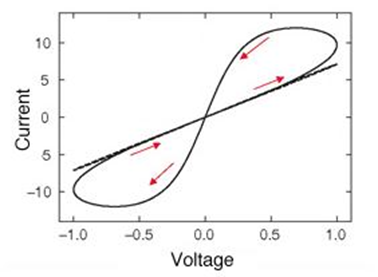
\includegraphics[width=0.45\textwidth]{Chapter1/Figs/1b.png}
    \caption[Spiking dynamics of a neuron.]{The action potential and the underlying conductance and currents with respect to time \cite{squire2012fundamental}. It should be noted that the increased conductance for $Na^+$ (and its inward flow) is associated with the rising phase of the action potential, whereas the slower increase in conductance for $K^+$ (and its outward flow) is associated with repolarisation of the membrane and with afterhyperpolarisation. The reduction in $I_{Na}$ before the peak of the action potential (even though $G_{Na}$ is still high) is due to inactivation of the Na+ channels.}
    \label{fig:1b}
\end{figure}

\noindent The combination of these factors renders it almost impossible for the neuron to fire during this time; this is referred to as the absolute refractory period. The change in ionic concentrations within the cell is relatively minor during a single spike, but over the course of numerous spikes, the ion pumps are required to maintain the optimal concentrations of sodium and potassium. Other currents, most notably calcium currents, are present in some neurons. \\

\noindent The rapid depolarisation associated with an action potential not only causes an increase in the somatic voltage potential, but also results in partial depolarisation of the axon segments situated in closer proximity to the soma. This results in the opening of sodium channels in that part of the axon, which in turn causes further depolarisation and the opening of sodium channels in the subsequent section of the axon. In this way, the somatic spike triggers a voltage wave that travels down the axon, eventually leading to the release of neurotransmitter(s) from synaptic vesicles situated near the ends of the axon. \\

% \noindent Axons are responsible for transmitting long-range signals in the brain, and thus exhibit considerable variation in length, contingent on whether a given neuron is connected to neighbouring neurons or to neurons situated in a different brain region. To facilitate long-range transmission, axons are coated in myelin, a substance composed mainly of lipids and thus a good electrical insulator.\\

% \noindent This enables the propagation of current down the axon. The high proportion of fat makes myelin white; bundles of axons are responsible for the "white matter" parts of the brain. In contrast, the "grey matter" is composed mainly of neuron dendrites, somas, and short-range axons.\\

% \noindent Dendrites are thin processes that extend away from the soma to connect to the axons of other neurons \cite{johnston1996active}. They serve to transmit current from synapses with other neurons to the soma. Initially, it was thought that they only conducted current passively; however, research has demonstrated that they possess active conductance mechanisms that are analogous to those involved in spike generation and propagation down an axon.\\

% \noindent Dendrites are also traditionally considered to act in a linear manner, whereby inputs from numerous synapses are accumulated over time and space. This remains a prevalent assumption in numerous computational models. However, recent studies have demonstrated that the summation of signals in dendrites is more intricate, exhibiting a combination of linear and nonlinear (sigmoidal) elements.\\

% \noindent Neurons are connected to one another by synapses, which facilitate the connection between the axon of the presynaptic neuron and a dendrite of the postsynaptic neuron. Upon the occurrence of a spike in the presynaptic neuron, an electrical pulse is transmitted along the axon, reaching the presynaptic terminals of all synapses situated along its length. The synaptic vesicles, which are filled with neurotransmitter, are located at the terminals. \\

% \noindent When an electrical pulse is generated, it causes the vesicles to release neurotransmitter into the synaptic cleft, which is the narrow space between the presynaptic terminal and the postsynaptic terminal. This neurotransmitter then activates receptors on the postsynaptic terminal, which open and permit the flow of current into the postsynaptic cell. The specific neurotransmitter utilized by the synapse is contingent upon the presynaptic neuron. \\

\noindent It has been established that all synapses located along a neuron's axon are responsible for the release of a singular neurotransmitter or a combination of neurotransmitters. This phenomenon is commonly referred to as Dale's principle. At the time of its development, Dale's principle was based on the assumption that each neuron produced a single type of neurotransmitter. Nevertheless, evidence of cotransmission was only discovered subsequently \cite{burnstock2004cotransmission}. It was understood that neurotransmitters can only be either excitatory or inhibitory,in relation to different postsynaptic cells.

\subsection[Spiking Neuron Dynamics]{Spiking Neuron Dynamics}

\noindent In recent times, the number of available neuron models has proliferated. The models currently in use in the literature range from the simplest possible rate-neuron model, namely binary threshold units \cite{stocks2001information}, to complex multi-compartmental models that account for detailed dendritic morphologies \cite{markram2015reconstruction}. In the context of large-scale neural models aiming to reproduce high-level behaviours, single-compartment neuron models remain the prevailing approach. \\

\noindent These models treat the neuron as a single electrical compartment, combining the dendrites, soma, and axon. In contrast, multi-compartmental models represent the neuron as comprising multiple electrical compartments, with equations that describe the influence of activity in one compartment on that of another. By modelling the spike separately from the rest of the neural dynamics, it is possible to separate time scales, thereby avoiding the need for additional computational resources to model the spike trajectory \cite{abbott1999lapicque}. \\

% \noindent The number of compartments in a model can vary considerably, from a minimalistic two-compartment structure, typically comprising one for the dendrites and one for the soma, to a more elaborate configuration comprising thousands of compartments. \\

% \noindent The number of compartments in a model is directly proportional to the amount of computing power required for simulation and the complexity of the resulting behaviour. For these reasons, models that seek to reproduce behaviour predominantly utilise either single-compartment neurons or simpler models that do not model the electrical activity of the neuron at all. \\

% \noindent Single-compartmental neuron models can be classified according to two key dichotomies: firstly, the rate-based versus spike-based dichotomy; and secondly, the static versus dynamic dichotomy. The distinction between rate-based and spiking neuron models concerns the nature of the output: is it a continuous value, represented by a firing rate, or a discrete value, represented by a spike.\\

% \noindent The distinction between static and dynamic models concerns the extent to which the model exhibits internal dynamics. In a static model, the output at a given point in time is independent of the neuron's past history and solely contingent on its instantaneous input. In contrast, a dynamic model allows for some degree of dependence on the neuron's past trajectory.\\

% \noindent Dynamic neuron models possess a state, which is to say, internal variables that evolve over time and are not directly computable from the present input to the model. They are typically expressed using differential equations. In contrast, static models output a function of the current input only; thus, they do not require differential equations to express them. \\

% \noindent It is important to note that the distinction between static and dynamic neurons does not necessarily refer to whether the neuron is being used as a static nonlinearity, evaluated at a single point in time on an input value, or as a dynamic nonlinearity, evaluated over a period of time on an input signal. \\

% \noindent Static neurons can be evaluated dynamically by evaluating them independently at each successive point in time on the input value. In contrast, there is no general method for evaluating dynamic neurons statically, as their input at any given point in time is contingent upon their internal state, which is a dynamic process that evolves over time. \\

% \noindent In some cases, it is possible to determine a firing rate response curve, also known as an I-F response curve or rate response function, for dynamic neuron models. This curve maps every constant value of the input current to a constant firing rate output. This can be determined analytically or empirically by applying a constant input current and measuring the rate of the output spikes, this can even be done in real neurons in vitro. \\

% \noindent However, many neuron models will not output spikes at a constant rate, even for a constant input, due to changing internal dynamics. In such cases, the rate-response function only captures part of the model, and will be different depending on the state of the model and how it is measured or calculated. \\

% \begin{table}[]
% \caption{Neuron Model Dichotomies.}
% \centering
% \begin{tabular}{|c|c|c|}
% \hline
%                  & \textbf{Rate}                                                                  & \textbf{Spiking}                                             \\ \hline
% \textbf{Static}  & Sigmoid Rate LIF                                                               & Poisson Spiking                                              \\ \hline
% \textbf{Dynamic} & \begin{tabular}[c]{@{}c@{}}Adaptive Rate LIF\\ Sigmoid with State\end{tabular} & \begin{tabular}[c]{@{}c@{}}Hodgkin-Huxley\\ LIF\end{tabular} \\ \hline
% \end{tabular}
% \label{table:4a}
% \end{table}

% \noindent Table \ref{table:4a} illustrates the manner in which a small selection of neuron models align with these dichotomies. In the static rate category, the models in question take in a continuous value and output a continuous function of that value. This encompasses the majority of non-linearities employed in machine learning (such as sigmoids or rectified linear units), in addition to the analytic firing rate for the LIF neuron model. \\

% \noindent In the static spiking category, models are characterised by the output of a discrete (binary) function of their continuous input. This category is primarily composed of Poisson-spiking neurons, which fire probabilistically based on their instantaneous firing rate. This implies that the probability of firing at a given time is independent of past firings. Furthermore, Poisson spiking can be applied to a dynamic rate model, whereby the probability of spiking is independent, but the spike rate is a dynamic process. \\

% \noindent Dynamic rate models possess an internal state that influences their continuous output, in addition to the input. This encompasses the analytic LIF rate model with adaptation, which possesses an intrinsic adaptation parameter that increases when the neuron is active and discounts the firing rate. Furthermore, the category encompasses sigmoid neuron models that possess an underlying voltage that is dynamically correlated with the neuron inputs \cite{lillicrap2016random}. \\ 

% \noindent The dynamic spiking category also includes the LIF neuron model, the Hodgkin-Huxley model, and more intricate multi-compartmental models. Within the category of spiking models, a distinction can be made between those that output instantaneous spikes (e.g., LIF) and those that output spikes that vary across time (e.g., Hodgkin-Huxley). Recently, another study have employed such models in the context of deep networks \cite{guerguiev2017towards}, subject to biological constraints. \\

% \noindent Another potential distinction can be made between models that output stereotyped spikes, where the size of each spike is identical, and those that output variable-sized spikes. Models of cortical neurons that output instantaneous spikes (e.g., LIF) almost invariably output stereotyped spikes. This is due to the fact that spikes in cortical neurons are almost identical in terms of magnitude, duration, and shape.\\

% \noindent It is widely believed that none of these factors carry information. Even among models that have spikes that vary across time (e.g., Hodgkin-Huxley), the spike magnitude, duration, and shape are quite consistent between spikes. Therefore, the majority of spiking cortical neuron models exhibit stereotyped spikes. \\

% \noindent By modelling the spike separately from the rest of the neural dynamics, it is possible to separate time scales, thereby avoiding the need for additional computational resources to model the spike trajectory, which is characterised by stereotyped details of little interest \cite{abbott1999lapicque}. \\

\begin{figure}[htbp!] 
    \centering    
    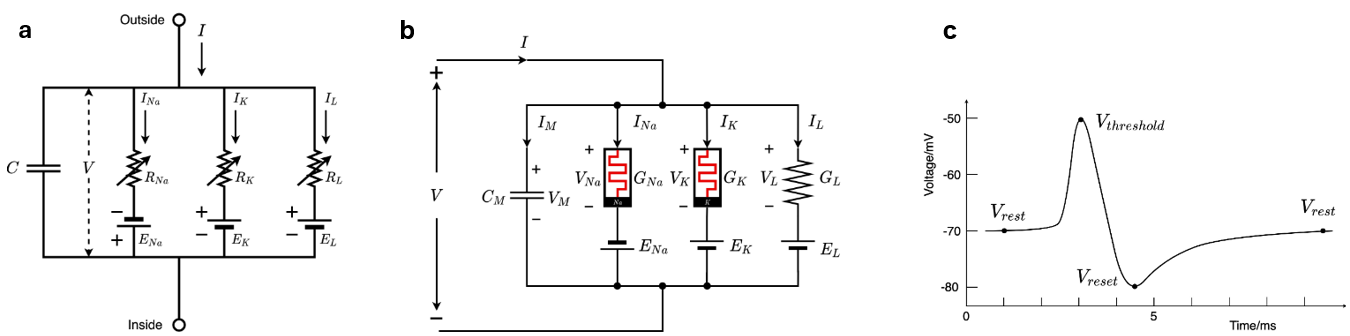
\includegraphics[width=1\textwidth]{Chapter1/Figs/1c.png}
    \caption[Hodgkin-Huxley neuron model.]{Hodgkin-Huxley neuron model. (a) An equivalent circuit for the HH models \cite{hodgkin1952quantitative}. (b) An equivalent circuit for memristive HH model \cite{chua2012hodgkin}. (c) An action potential waveform, which demonstrates the resting, threshold, and reset potentials. }
    \label{fig:1c}
\end{figure}

\noindent A significant proportion of the most influential findings in computational neuroscience are based on mathematically detailed models of neuronal functioning. One of the most renowned of these is the Hodgkin-Huxley model of the squid giant axon \cite{hodgkin1952quantitative}. the Hodgkin–Huxley (HH) model is one of the most widely used, comprising a set of nonlinear differential equations that accurately approximate the electrical signals of neurons \cite{chua2012hodgkin}. \\

\noindent Figure \ref{fig:1c}(a) depicts the HH neural model, wherein the time-varying nonlinear conductor $R_{Na}(GNa)$ and $R_K(G_K)$ represent the sodium and potassium channels, respectively, while the linear conductor $R_L(G_L)$ simulates leak channels and $C$ models the membrane of a neuron. The equations of the HH model are presented below: 
\begin{align}
    C \frac{dV_m(t)}{dt} = I_C(t) + \sum_{k}^{}I_k(t) \label{eq:1.1} 
\end{align}

\noindent In this context, $V_m$ represents the membrane potential. $\sum_{k}^{}I_k(t)$ denotes the sum of the ionic currents flowing into the neuron. This can be formulated by three ion currents, as follows:
\begin{align}
    \sum_{k}^{}I_k &= C_m \frac{dV_m}{dt} + G_Kn^4(V_m - V_K) + G_{Na}m^3(V_m - V_{Na}) + G_L (V_m - V_L) \label{eq:1.2} \\
    \frac{dn}{dt} &= \alpha_n(V_m)(1-n)-\beta_n(V_m)n \label{eq:1.3} \\
    \frac{dm}{dt} &= \alpha_m(V_m)(1-m) - \beta_m(V_m)m \label{eq:1.4} \\
    \frac{dh}{dt} &= \alpha_h(V_m)(1-h)-\beta_h(V_m)h \label{eq:1.5}
\end{align}

\noindent The reversal potentials $V_K$, $V_{Na}$, and $V_L$ are the three parameters in question. The rate constants $\alpha_i$ and $\beta_i$, which depend on the membrane potential, describe the behaviour of the $i^{th}$ ion channel. The maximal value of the conductance is represented by $G_K$, $G_{Na}$, and $G_L$. \\

\noindent Finally, the dimensionless quantities \textit{n}, \textit{m}, and \textit{h}, which lie between 0 and 1, are associated with three ion channels. In order to achieve the optimal fit for human action potentials, the HH model is reduced by setting the leakage channel conductance to $G_L = 0$  \cite{noble1962modification}.It has been demonstrated that $G_{Na}$ and $G_K$ are memristors \cite{chua1976memristive}, in the equivalent circuit in figure \ref{fig:1c}(b). \\

\noindent The integrate-and-fire (IF) neuron \cite{lapicque1907louis} constituted one of the earliest computational models of a neuron. This model was developed prior to the ability of researchers to measure the electrical and chemical changes occurring in a functioning neuron. It is based on the premise that the neuron membrane can be modelled as a capacitor that stores charge over time \cite{abbott1999lapicque}.\\

\noindent As the name suggests, the IF model exhibits two principal behaviours: The model integrates current over time, as would be expected of a capacitor, and fires when the voltage reaches a threshold. Furthermore, the model may or may not incorporate a leak term, which represents a resistor in parallel with the capacitor that permits the dissipation of charge over time. The model with a leak term is typically designated as the leaky integrate-and-fire (LIF) model. While the term "integrate-and-fire (IF) model" can be used interchangably. \\

\noindent To identify how the neuron's membrane voltage evolves over time and, based on this, to determine when the neuron spikes, the charge \textit{Q} across a capacitor is represented by $Q = V \times C$, where \textit{V} is the voltage across the capacitor and \textit{C} is the capacitance. By differentiating this with respect to time, the membrane voltage $\textit{V(t)}$ of the neuron is:
\begin{align}
    C \frac{dV(t)}{dt} = J(t) \label{eq:1.6} 
\end{align}

\noindent In this context, \textit{J(t)} represents the input current to the neuron over time, whereas \textit{C} denotes the membrane capacitance. The current here is the time derivative of charge. Equation \ref{eq:1.6} demonstrates that the IF neuron simply integrates the input current over time. It is still necessary to identify the point at which the neuron spikes. \\

\noindent This is achieved by defining a threshold voltage, $V_{th}$, which is exceeded when the voltage passes this threshold, resulting in the neuron firing. This is a fundamental principle in neurophysiology: once the neuron voltage passes a threshold, the neuron begins firing a spike, and once this firing process begins, it is almost impossible to reverse. \\

\noindent Once a neuron has fired a spike, the membrane voltage is reset to the resting potential, $V_{rest}$. This phenomenon can be attributed to physiological resetting procedures. Following the occurrence of a spike in a neuron, other ionic currents, typically potassium, are initiated, leading to a restoration of the membrane voltage towards the resting potential.\\

% \noindent Some integrate-and-fire models may also incorporate an absolute refractory period, defined as a time interval during which the voltage is maintained at the resting potential $V_{rest}$ following a spike. In cortical neurons, post-spike potassium currents are sufficiently strong to prevent another spike from occurring for a considerable duration. This time interval is referred to as the absolute refractory period. The model accounts for this by holding the membrane voltage at $V_{rest}$ for a duration equal to the absolute refractory period. \\

\noindent The leaky integrate-and-fire (LIF) model \cite{knight1972dynamics} incorporates an additional physiological factor: Neuron membranes are not perfect capacitors; rather, they slowly leak current over time, pulling the membrane voltage back to its resting potential. Therefore, the membrane is modelled as a capacitor and resistor in parallel, which allows for the neuron to exhibit a degree of "forgetting": in the absence of any input, the membrane voltage will return to its resting potential \cite{koch2004biophysics}. The LIF dynamics are captured by the following equation:

\begin{align}
C \frac{dV(t)}{dt} = J(t) - \frac{1}{R} (V - V_{rest}) \label{eq:1.7} 
\end{align}

\noindent In this model, \textit{R} represents the membrane resistance, and the remaining parameters are consistent with those of the IF model, with identical resetting procedure.\\

\noindent The LIF model comprises a number of parameters, including $C, R, V_{rest}$ and $V_{th}$. It is possible to normalise the model in order to reduce the number of parameters while maintaining the full dynamics of the original model. In particular, the model can be manipulated so that the normalised voltage lies within the range [0, 1], with a normalised resting potential of zero and a normalised firing threshold of one. Initially, Equation \ref{eq:1.7} is multiplied by R to give:

\begin{align}
    \tau_{rc} \frac{dV}{dt} &= RJ(t) - V + V_{rest} \label{eq:1.8} \\
    \tau_{rc} &= R \times C \label{eq:1.9} \\
    \bar{V} &= \frac{V - V_{rest}}{V_{th} - V_{rest}} \label{eq:1.10} \\
    \bar{V_{rest}} &= \frac{V_{rest}}{V_{th}} \label{eq:1.11} 
\end{align}

\noindent By substituting $\bar{V}$ and $\bar{V_{rest}}$ into equation \ref{eq:1.3} to give:


\begin{align}
    \tau_{RC}(V_{th} - V_{rest})\frac{d\bar{V}}{dt} &= RJ(t) - \bar{V}(V_{th} - V_{rest})
    \label{eq:1.12} \\
    \tau_{rc}\frac{d\bar{V}}{dt} &= \frac{R}{V_{th} - V_{rest}} J(t) - \bar{V} \label{eq:1.13} \\
    \tau_{rc} \frac{d\bar{V}}{dt} &= \bar{J}(t) - \bar{V} \label{eq:1.14} 
\end{align}

\noindent When the firing threshold for the new equation $\bar{V_{th}} = 1$, the voltage resets to $\bar{V_{rest}} = 0$, and $\bar{J}(t) = \frac{R}{V_{th} - V_{rest}} J(t)$. It can be observed that $\bar{J}(t)$ is merely a linear transformation of $J(t)$. Consequently, (\ref{eq:1.14}) retains the full dynamics of (\ref{eq:1.7}) for a scaled input, but with only one parameter, $\tau_{RC}$. \\

\noindent It should be noted that both $\bar{V}$ and $\bar{J}$ are unitless quantities. Conventionally, the unitless space is employed exclusively, and the quantities are often referred to simply as \textit{V} and \textit{J}, despite the fact that they are not voltages or currents. This simplifies the mathematical representation, without limiting the generality of the models. \\

\noindent (\ref{eq:1.14}) provides an exact description of the circumstances under which the model neuron will spike in response to a given input current, \textit{J(t)}. However, in some cases, it is sufficient to consider only the spike rate, that is, the number of spikes per second that the neuron will produce in response to a given input current. \\

\noindent In the case of the LIF model, it is possible to determine the analytical firing rate for a constant input current. This is achieved by calculating the inter-spike interval (ISI), which is the time between one spike and the next. The firing rate is then given by the inverse of the ISI. When a constant input current, $J(t) = j$, is provided, it is possible to solve (\ref{eq:1.14}) in order to find the neuron voltage over time. 
\begin{align}
    V(t) = (V(0) - j)e^{\frac{-t}{\tau_{rc}}} + j \label{eq:1.15}
\end{align}

\noindent In the absence of spikes, the objective is to ascertain the time required for the voltage to increase from$ V(0) = 0$ to $V(t) = 1$. This property will only occur if $j > 1$. Substitution into (\ref{eq:3.15}) and subsequent solution for \textit{t} yields:
\begin{align}
    t = - \tau_{RC} log \left( - \frac{1}{j} \right) \label{eq:1.16}
\end{align}

\noindent Incorporating the refractory period and performing the inversion, the spike rate \textit{r} for the LIF neuron is given by:
\begin{align}
    r &= \begin{cases}
    \frac{1}{t_{ref} - \tau_{RC} log \left( 1 - \frac{1}{j} \right)} & \text{ if } j > 1 \\ 
    0 & \text{ otherwise }  
    \end{cases} \label{eq:1.17}
\end{align}


\noindent The LIF model is one of the most widely utilised simplified neuron models \cite{lapique1907researches}. The simple equivalent model is illustrated in Figure \ref{fig:1d}(a). In this model \cite{stein1967frequency}, a resistor \textit{R}, connected in series with a \textit{DC} source $V_{rest}/V_{reset}$, is connected in parallel with a capacitor \textit{C}. A postsynaptic neuron receives a synaptic current \textit{I(t)}, generated by presynaptic spikes. \\

\noindent A proportion of the current \textit{I(t)} flowing into \textit{C} results in an increase in the membrane potential \textit{V(t)}. The charge leakage occurs via resistor \textit{R}. When \textit{V(t)} reaches a threshold value, the neuron generates a spike. Following the generation of a spike, the membrane potential is reset to the reset value. \\

\noindent In the absence of \textit{I(t)}, the voltage across \textit{C} is eventually settled at $V_{rest}$, representing the cell's resting potential. During the refractory period $t_0$, a neuron is incapable of spiking. Figure \ref{fig:1d}(c,d) illustrates the LIF neuron dynamics for the case of a \textit{DC} input current and a zero rest and reset potential, $E_{reset} = E_{rest} = 0$ \cite{tal1997computing}. \\

\begin{figure}[htbp!] 
\centering    
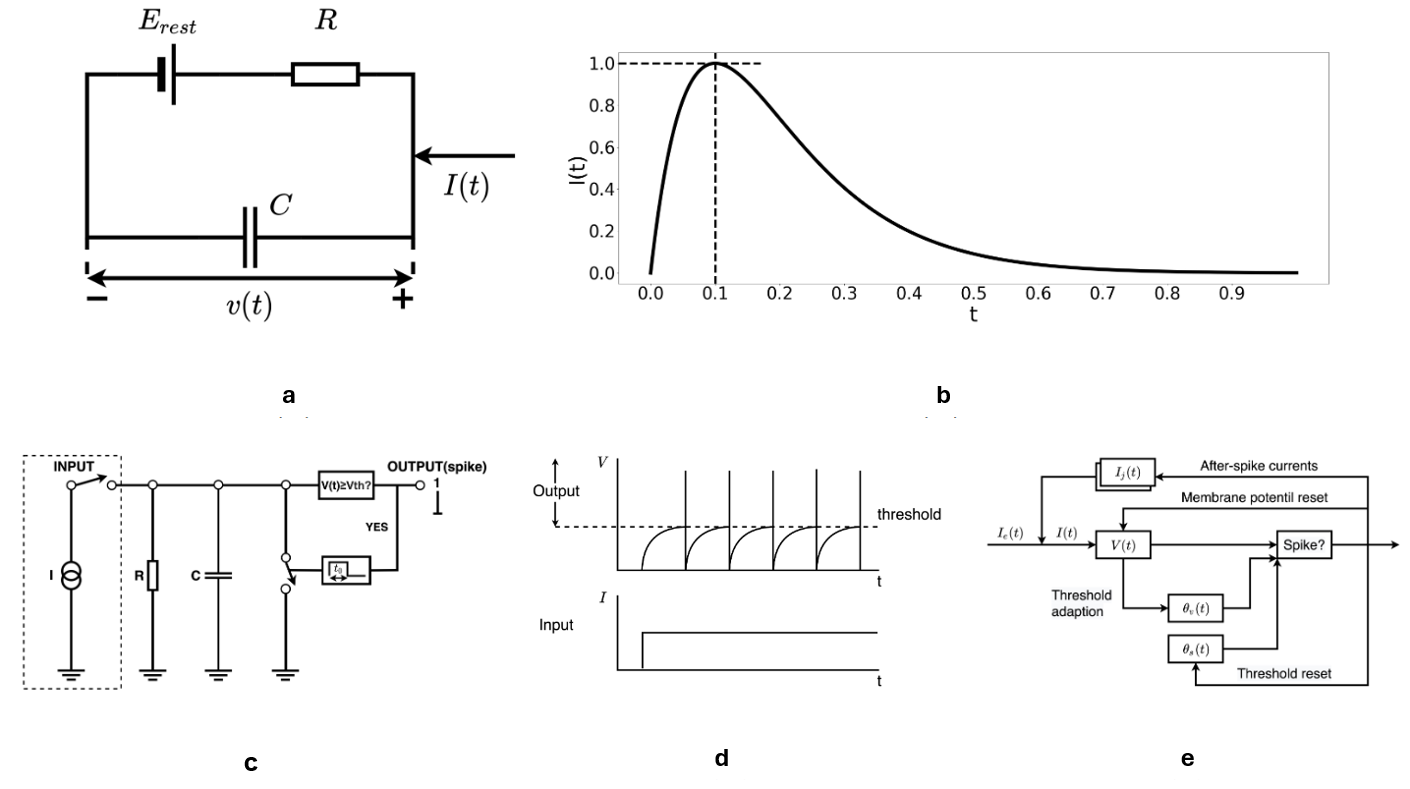
\includegraphics[width=1\textwidth]{Chapter1/Figs/1d.png}
\caption[The Leaky Integrate-and-Fire neuron model.]{The LIF neuron model. (a) Schematic diagram of the LIF electrical model. (b) Input current in the form of an alpha function, $\tau_{\alpha} = 0.1, I_0 = 1$ (c)The LIF model allows for the control of spiking behaviour through a comparison of membrane potential and threshold at each time step. Upon the triggering of a spike, a voltage-controlled switch discharges C for a duration corresponding to the refractory period $t_0$ \cite{tal1997computing}. (d) A simulation of constant firing frequency for DC current input in which $t_0$ is hidden. DC input current and output spikes are both shown. (e) A generalised LIF model with threshold control \cite{teeter2018generalized}. }
\label{fig:1d}
\end{figure}

\noindent The input synaptic current, \textit{I(t)}, can be described by a time-varying alpha function. However, alternative functions may be employed, including "Instantaneous Rise and Single Exponential Decay," "Biexponential Functions," "Sawtooth," and "Pulse Function." The alpha synaptic current is modeled by Equation \ref{eq:3.15}, and the resulting plot is shown in Figure \ref{fig:4b}(b). \\

\noindent Nevertheless, Figure \ref{fig:3d}(a) lacks a circuit for resetting the system when the threshold is reached. In order to evaluate the inequality $V > V_{threshold}$, it is necessary to use an active circuit, such as a comparator. Upon reaching the threshold, the membrane potential must be reset in accordance with the illustration in Figure \ref{fig:3d}(d). Therefore, the LIF model's generalized version necessitates additional overhead, as illustrated in Figure \ref{fig:3d}(e). \\

% \noindent In the generalized LIF model, the reset behavior necessitates external control to pull down the membrane potential below the resting potential. This external control requires intricate, active circuits comprising MOS transistors, resistors, and even a silicon-controlled rectifier (SCR), which represents a significant drawback in a neuromorphic system due to its substantial power and area consumption. \\

% \noindent In order to address the limitations of conventional neuron models, memristor technologies can be employed to emulate biological neurons with the objective of reducing energy consumption and increasing packing density. The HH model has been emulated by utilising two memristors in parallel with two capacitors, respectively mimicking two channels that are coupled to each other with a resistor. \\

% \noindent Additionally, an input resistor and an output impedance comprising a resistor and a capacitor have been proposed \cite{pickett2013scalable}. The LIF neuron has been demonstrated using a diffusive/volatile memristor in parallel with a capacitor, and the neuron has been employed in a fully memristive neural network \cite{wang2018fully}. \\

% \noindent Despite the existence of memristor-based neuron models, the lack of accessible experimental data and hardware for prototyping memristive circuits represents a significant obstacle. A significant number of state-of-the-art experimental demonstrations have relied on bespoke fabrication processes that cannot be reproduced using off-the-shelf memristors. \\

% \noindent Furthermore, the limited choice of commercially available, low-cost, discretely packaged memristors, which are known to be highly sensitive and stochastic in behaviour, has compounded the issue. The challenge in developing hardware prototypes has made it difficult to perform experimental validation. \\

% \noindent In addition to the acceleration of neural networks, the design of a solid-state brain that can harness the neural code has gained increasing attention as a means of processing vast quantities of sensory data without being constrained by the von Neumann bottleneck. The solid-state brain is structured in a manner that emulates the cerebral cortex, with neurons interconnected by a vast array of variable synapses. \\

% \noindent It is hypothesised that neurons and synapses can be realised with memristors integrated with a complementary metal-oxide semiconductor (CMOS) process. However, the design of a large-scale solid-state brain remains elusive in neuromorphic computing due to the considerable overheads associated with mimicking the surface area of neural tissue, constrained power consumption, routing, and the massive parallelism of synaptic connections.

\noindent It is evident that neurons manifest considerable heterogeneity with regard to their dynamics, morphology and connectivity. They can summarily be categorised as follows: Excitatory neurons are responsible for promoting activity in connected neurons. In contrast, inhibitory neurons are responsible for suppressing activity, a process that is crucial for stability and rhythm. Finally, interneurons connect local circuits, thereby enabling complex computations.

\subsection[Synaptic Transmission and Plasticity]{Synaptic Transmission and Plasticity}

Prior to model internal neural dynamics, it is essential to model the dynamics of the synapses that connect neurons to one another. Synapses exert a significant functional effect as a low-pass filter on the spikes that pass through them. A spike in the presynaptic neuron elicits an extended current pulse in the postsynaptic neuron. This pulse can be conceptualised as a low-pass filtered version of the presynaptic spike. \\

\noindent The simplest model of a synapse is that of a first-order low-pass filter. The impulse response of a filter describes the manner in which the filter responds to an infinitesimally short input of unit integral, which is called an impulse. This idealised impulse is also a reasonable model of a spike, and thus the impulse response also describes what the postsynaptic current will look like in response to a presynaptic spike. The impulse response of the first-order low-pass filter is as follows:
\begin{align}
h(t) = \frac{1}{\tau_s}e^{\frac{t}{\tau_s}} \label{eq:1.18} 
\end{align}

\noindent The synaptic time constant, denoted by $\tau_s$, is defined as the length of time over which the postsynaptic current is spread. Given that the impulse response is an exponential function, the exponential synapse model is therefore a suitable description.
\begin{align}
h(t) = \frac{1}{\tau_s^2}e^{\frac{t}{\tau_s}} \label{eq:1.19} 
\end{align}

\noindent It was determined that a second-order lowpass filter is a superior model for a synapse \cite{mainen1995reliability}. The impulse response of this filter is defined by (\ref{eq:1.19}). This function is referred to as the alpha function, and thus the model is designated as the alpha synapse model. Both of these models are based on the current generated by a spike in the postsynaptic neuron, which is a current-based synapse model.\\

% \noindent Other current-based synapse models exist; a popular one is the double-exponential model, which is similar to the alpha synapse but with two time constants, thereby affording greater control over the rise and fall of the impulse response. Where The double-exponential model with both time constants set to the same value reduces to the alpha synapse. \\

% \noindent Many of the other, more realistic synapse models are conductance-based, meaning that they model the conductance of the neural membrane at the synapse. The current flowing into the neuron is dependent on both the conductance and the voltage across the membrane. The latter undergoes a change as the synapse becomes active. \\

% % \subsection[Neural Coding Schemes]{Neural Coding Schemes}

\noindent One of the primary objectives of computational neuroscience is to ascertain the manner in which the brain represents—or encodes—information. To this end, researchers have put forth a multitude of potential coding schemes that neurons could utilise for information encoding. One key distinction between rate coding and temporal coding is the following dichotomy. \\

\noindent In a rate code, the sole pertinent measure is the firing rate (i.e. the number of spikes) of a neuron over a given period of time. An exemple of a rate code is motor neurons in the peripheral nervous system. The contraction of a muscle is contingent upon the number of spikes per unit time; thus, only the rate of motor neuron spikes is significant \cite{gerstner1997neural}. In a temporal code, the time of individual spikes is also a factor. For example, in the early auditory system, precise spike timing facilitates the localisation of sounds \cite{chase2006spike}.\\

\noindent The precise definitions of rate and temporal codes remain contentious, with differing interpretations presented by various authors \cite{dayan2005theoretical}. To illustrate, a neuron may discharge a number of spikes in rapid succession, followed by a period of quiescence. A second neuron may be observed to fire the same number of spikes, but in a more evenly distributed manner over a given period. \\

% \noindent One possible interpretation is that both neurons have the same firing rate, but the first has all its spikes occurring near the beginning of the period, in which case the timing of the spikes is a significant factor. An alternative perspective posits that the instantaneous firing rate of the first neuron fluctuates over the period, whereas that of the second neuron remains constant. This suggests that it is the instantaneous firing rate, rather than the overall firing rate, that is of primary importance. \\

% \noindent This highlights a limitation of solely examining the overall firing rate (i.e., the number of spikes) of a neuron over a given period. It is unclear which period should be considered. In real neurons, the period of time that is relevant for counting spikes depends on parameters such as the membrane time constant tau of the postsynaptic neuron. \\

% \noindent For this reason, neuroscientists will often differentiate between rate and timing codes based on the frequency of alterations in the instantaneous firing rate. If the rate of firing exhibits rapid fluctuations, and if these fluctuations contain information about the stimulus (and are not simply spurious variation or "noise"), then the code is said to be temporal; otherwise, it is a rate code. \\

% \noindent Once again, there is a lack of consensus regarding the minimum frequency of fluctuations in firing rates that must be observed to qualify as temporal codes. One possible definition is relative to the stimulus. The firing rate of neurons can be triggered to change rapidly in response to fast-changing stimuli, regardless of whether the code in use is rate or temporal. \\

% \noindent If the temporal code is defined as having meaningful firing rate fluctuations at a faster time scale than changes in the stimulus, then it can be differentiated between codes that have fluctuations because they are using them for coding and those that simply have fluctuations triggered by the stimulus. According to this definition, neurons using a temporal code will have a fluctuating firing rate in response to a constant stimulus, whereas neurons using a rate code will have a non-fluctuating firing rate. \\

\noindent Both rate codes and temporal codes describe the encoding properties of individual neurons. Additionally, one may inquire about the coding properties of a group (also known as a population) of neurons. The concept of population coding pertains to instances where a representation is distributed across numerous neurons within a population, such that the represented value cannot be decoded from the activities of a limited number of neurons.\\

\noindent The simplest method of extrapolating the concept of rate or temporal coding to multiple neurons would be to have numerous neurons all implementing the same code. In other words, all neurons will exhibit a similar firing pattern when representing a given value, due to their comparable tuning properties. This results in a significant degree of redundancy between neurons. \\

\noindent In contrast, population coding entails each neuron representing a distinct aspect of the represented value. To illustrate, if the objective is to represent head direction, there are neurons that represent a head that is fully turned to the left, others that represent a head that is fully turned to the right, and still others that represent a centred head. Additionally, there are neurons that represent values in between these three head directions. The direction in which a neuron is most active is referred to as its preferred direction. \\

% \noindent It should be noted that each neuron exhibits some degree of variance, whereby it will fire for head directions that are relatively close to its preferred direction. Conversely, the further the actual head direction is from a neuron's preferred direction, the less it will fire. By utilising the activities of all neurons in the population, it is possible to decode the head direction with a high degree of accuracy. \\

% \noindent From a population perspective, it is possible to differentiate between codes that exploit synchrony between neurons and those that do not. This can be facilitated, for example, by coincidence detection, whereby a postsynaptic neuron will only fire if the spikes of two of its input neurons are coincident, that is to say, they fall within the same (small) temporal window. \\

% \noindent This distinction between temporal and rate coding schemes is further exemplified by the fact that only temporal codes can take advantage of correlations between individual spikes of neurons. Rate coding schemes, on the other hand, can only take advantage of synchrony between neurons in terms of synchronised fluctuations of their instantaneous firing rates, since they lack the temporal precision to co-ordinate individual spikes.

\noindent Synapses are therefore known to play a dual role in the nervous system. They facilitate communication between neurons and serve as the primary locus of learning and memory. The magnitude of this influence, or 'synaptic strength' \cite{bastos2022motor}, is determined by the relative strength of the connection between the presynaptic and postsynaptic neurons. This phenomenon is known as synaptic plasticity. \\

\noindent It is important to note that plasticity can be categorised into several distinct types. Short-Term Plasticity (STP): Transient changes that last from milliseconds to seconds. Long-Term Potentiation (LTP) and Long-Term Depression (LTD): The phenomenon of sustained increases or decreases in synaptic strength over time. \\

\noindent The most significant model of synaptic plasticity is Hebbian learning, which can be succinctly summarised as follows: The hypothesis that neurons that fire together wire together has been proven to be accurate. A more precise, temporally-sensitive rule is Spike-Timing Dependent Plasticity (STDP) \cite{zheng2018learning}. \\

\noindent Mathematical Models can capture the effect of precise spike timing on synaptic weight updates. If a presynaptic neuron fires before a postsynaptic neuron within a short window, the synapse is strengthened; if the order is reversed, the synapse weakens. A common representation for this is:
\begin{align}
\Delta w = \left\{ \begin{array}{cl}
    A_+ \cdot e^{-\Delta t/\tau_+}, & \ \Delta t > 0 \\
    -A_- \cdot e^{-\Delta t/\tau_-}, & \ \Delta t < 0
    \end{array} \right. \label{eq:1.20}
\end{align}

\noindent Where $\Delta t = t_{post} - t_{pre}$ is the timing difference, $A_+, A_-$ are learning rates, $\tau_+, \tau_-$ are time constants for potentiation and depression. This asymmetric window is indicative of experimental observations and provides a biologically plausible basis for synaptic learning in hardware.\\

\noindent As a small primer, memristive devices offer an electronic analogue to synapses due to their tunable conductance and memory of past activity. When configured in crossbar arrays, these devices have the capacity to implement synaptic weight matrices directly in hardware, with updates governed by local voltage or current pulses.\\

\noindent Memristive STDP implementations frequently exploit device physics, where conductance change is contingent on pulse overlap:
\begin{align}
    \Delta G = f(V_{pre}, V_{post}, \Delta t) \label{eq:1.21}
\end{align}
\noindent where $f$ is a device-specific function determined by material properties and pulse shapes. \\

\noindent It is important to note that memristors have the capacity to inherently facilitate the nonlinear, history-dependent behaviour that is characteristic of biological plasticity rules, such as STDP. To illustrate this point, the application of carefully timed voltage pulses to a memristor has been demonstrated to result in an increase or decrease in conductance, respectively, reminiscent of LTP and LTD.

\section[Foundations of Neuromorphic Computing]{Foundations of Neuromorphic Computing}

Neuromorphic computing signifies a paradigm shift of the manner in which information is processed and stored; this is inspired directly by the architecture and function of biological neural systems. Conventional computing systems compartmentalise memory and processing units, a configuration that engenders energy and velocity inefficiencies due to incessant data movement. Neuromorphic systems are designed to co-locate memory and computation by leveraging distributed, parallel architectures that emulate the brain's functionality.

\subsection[Memristor Fundamentals]{Memristor Fundamentals}

Memristive devices, also known as memory resistors, are emerging as foundational elements in neuromorphic computing due to their ability to retain resistive states based on electrical history, thereby emulating biological synapses. The central purpose of these components is to facilitate both memory storage and computation within a unified, compact structure, thereby enabling the co-location of memory and processing elements that is vital for brain-inspired architectures.

\subsection[From Biological Inspiration to Silicon Realization]{From Biological Inspiration to Silicon Realization}

\subsection[Encoding Plasticity in Memristors]{Encoding Plasticity in Memristors}

\section[Architectures and System-Level Integration]{Architectures and System-Level Integration}

\subsection[Hierarchical Modular Architectures]{Hierarchical Modular Architectures}

\subsection[Hardware-Software Co-Design]{Hardware-Software Co-Design}

\subsection[Experimental Validations Structure]{Experimental Validations Structure}

\section[Summary]{Summary}
%!TEX root = ../thesis.tex
%*******************************************************************************
%*********************************** First Chapter *****************************
%*******************************************************************************

\chapter{Theoretical Foundations}  %Title of the First Chapter


\section[Neuroscience Primers]{Neuroscience Primers}

\noindent Computational neuroscience employs a computational methodology to elucidate the mechanisms underlying brain function. This entails not only identifying the computations performed by the brain but also understanding the interactions between brain elements, such as neurons and synapses, that facilitate these computations.\\

% \noindent The field of computational neuroscience has traditionally adopted a bottom-up approach, commencing with the study of individual neurons and subsequently examining how these can be integrated into progressively larger networks, ultimately leading to the emergence of meaningful behaviour. \\

% \noindent In contrast, psychology and cognitive science have adopted a more top-down approach, commencing with the observation of animal behaviour and subsequently attempting to elucidate the brain mechanisms underlying these behaviours in terms of the higher-level functions of large brain areas. \\

% \noindent This distinction has resulted in a historical focus on developing comprehensive mathematical models of individual neurons and small- to medium-sized networks in computational neuroscience. Recently, however, there has been a convergence with other fields, leading to the creation of neurally detailed models capable of reproducing organism-level behaviors. \\

\noindent The brain is capable of performing a vast array of computations, with the fundamental units of the brain generally considered to be neurons and synapses. In the context of the nervous system, a synapse is defined as a structure that is capable of facilitating the transfer of an electrical or chemical signal from a presynaptic neuron to a postsynaptic neuron. \\

% \noindent In the case of a chemical synapse, the occurrence of a spike in the presynaptic neuron will result in the stimulation of the release of a chemical substance known as a neurotransmitter. Subsequently, the neurotransmitter will migrate to bind with the receptors in the membrane of the postsynaptic neuron. \\

% \noindent The effects of different neurotransmitters vary, exerting excitatory or inhibitory effects on the postsynaptic neurons. Many receptors contain different ion channels, which permit ions to flow between the inside and outside of the membrane, thereby generating an excitatory postsynaptic current (EPSC) or an inhibitory postsynaptic current (IPSC). \\

\noindent This section provides a concise overview of the relevant biological details, in addition to the concepts and models from computational neuroscience that are employed or expanded upon in this study. These details provide invaluable preliminary information for accurately modelling the implementation of silicon oxide device-based neuromorphic hardware and bio-inspired computing. \\

\noindent 
In addition to the fundamental biological details that are pertinent to the subject under discussion, the section provides information both at the neural level and at the network level. It is important to acknowledge that the models outlined in this study are comparatively rudimentary when placed in contrast to the substantial corpus of evidence that has been amassed on the neural system. This extensive body of evidence \cite{kandel2000principles}, constitutes the preponderance of neural data concerning these domains. Consequently, this section presents only the most fundamental biological facts relevant to the present work.


\subsection[Neuron Anatomy and Electrophysiology]{Neuron Anatomy and Electrophysiology}

\noindent  A neuron is a specialised biological cell that processes and transmits information through electrical and chemical signals \cite{mel1994information}. They represent only one of the numerous cell types within the brain, yet they are the most frequently discussed due to their status as the primary computational entities. Their fundamental function is relatively straightforward: neurons receive input from other neurons, and if that input is sufficiently stimulating, they will fire an action potential (also known as a spike), which propagates to other neurons.\\

\noindent Figure \ref{fig:2a} illustrates the basic structure of a neuron. Neurons can be subdivided into three principal parts: the dendrites, the cell body (soma), and the axon. Neurons receive input currents via their dendrites, which then transmit or channel this into the cell body, called the soma. When a neuron spikes, it sends current down its axon, which results in the release of neurotransmitter(s) at the synapses. These are connections from a neuron's axon to the dendrites of other neurons, and the neurotransmitter release causes dendritic input currents in these other connected neurons. \\

\begin{figure}[htbp!] 
    \centering    
    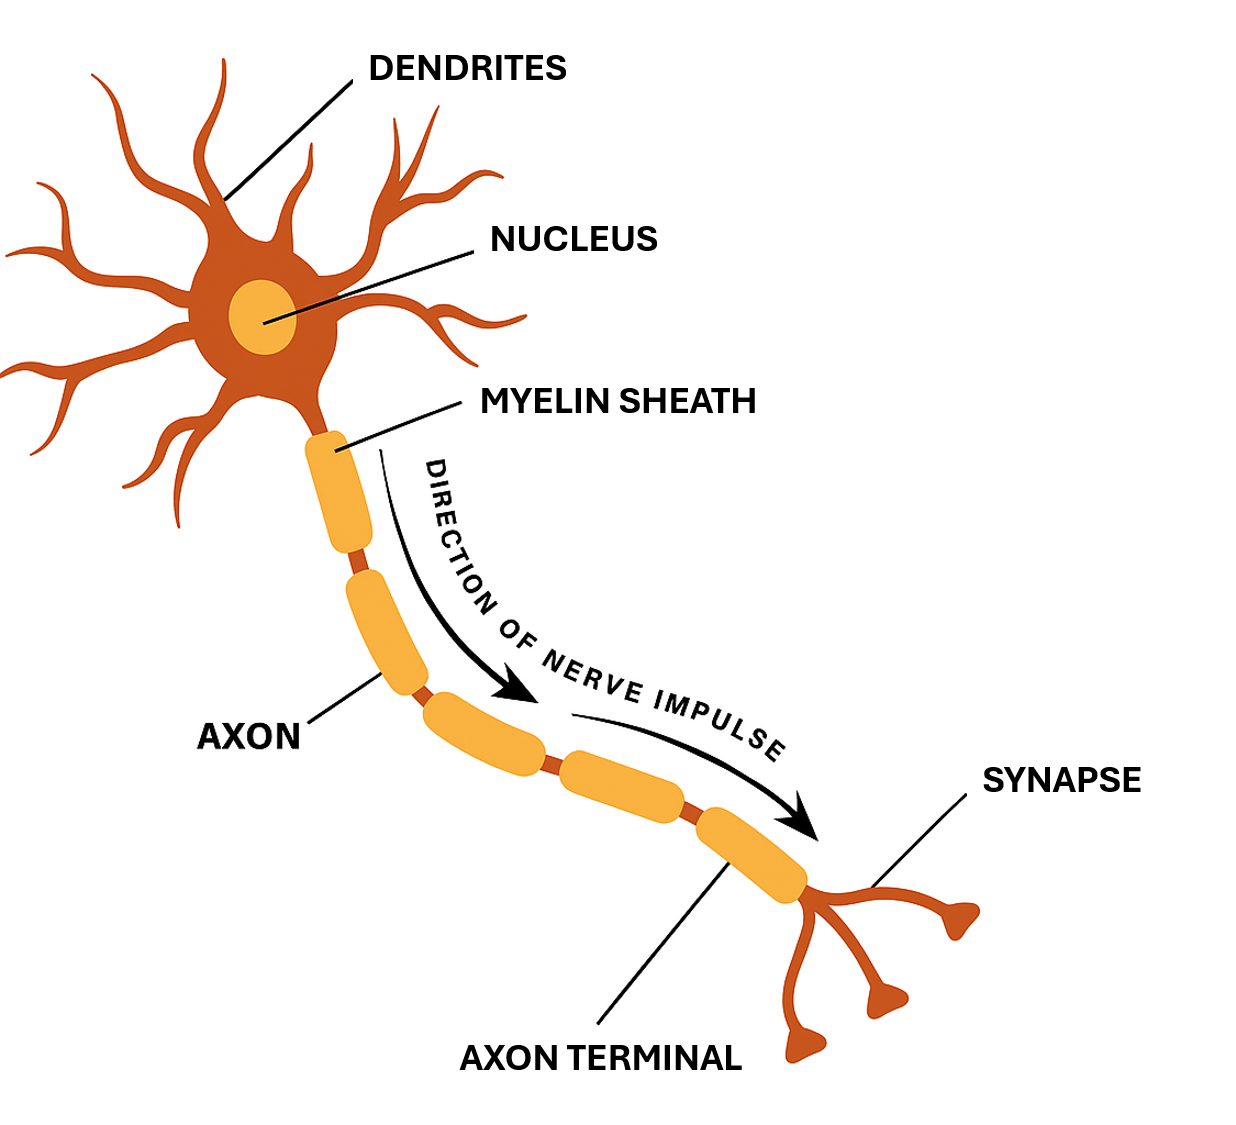
\includegraphics[width=0.5\textwidth]{Chapter2/Figs/a.png}
    \caption[Labeled diagram of the neuron.]{Labeled diagram of the neuron, nerve cell that is the main part of the nervous system. A neuron's dendrites include synapses that allow it to accept input from other neurons. The dendrites carry current to the soma, which is where electrical charge is integrated. If the neuron membrane gets sufficiently polarised, an action potential (also known as a spike) travels down the axon. This causes neurotransmitters to be released at synapses, resulting in currents in the dendrites of postsynaptic neurons.}
    \label{fig:2a}
    \end{figure}

\noindent From a computational perspective, the soma represents the integration point for all incoming currents from dendrites \cite{polsky2004computational}, marking the initiation of the action potential generation process (Figure \ref{fig:2b}). When a neuron is at rest, the soma exhibits a negative charge. This is referred to as the resting voltage and is maintained by ion pumps that regulate the concentration of ions (predominantly sodium, $Na^+$, potassium, $K^+$, and calcium, $Ca^{+2}$) within the cell. \\


\noindent As the currents arrive from the dendrites, they initiate a process of depolarisation of the cell \cite{johnston1996active}. Once the voltage within the soma reaches a sufficient level, it initiates the opening of voltage-activated sodium channels, which permit the influx of sodium ions into the cell, further depolarising it. This process persists until the electrical gradient resulting from the accumulation of sodium ions reaches a point where it is no longer in equilibrium with the chemical gradient caused by the imbalance of sodium within and outside the cell. This leads to a notable increase in the neuron's positive charge, exceeding the resting voltage. \\

\noindent Furthermore, this substantial depolarisation also activates voltage-gated potassium channels, which subsequently permit the release of potassium ions from the cell, thereby facilitating repolarisation. Concurrently, the sodium channels undergo inactivation. The opening of potassium channels ultimately results in the cell reaching a voltage below its resting level, a state known as hyperpolarisation. The sodium channels remain inactivated and the potassium channels remain open for a period of time following the spike. \\

\begin{figure}[htbp!] 
    \centering    
    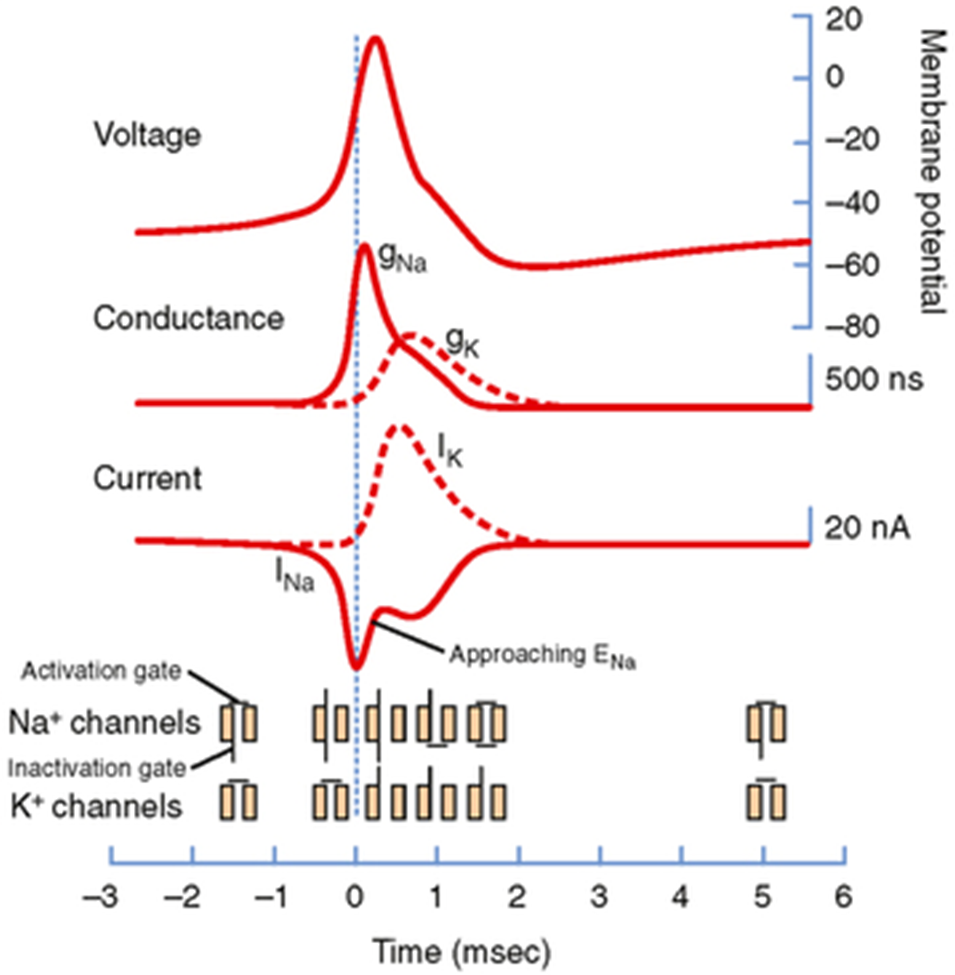
\includegraphics[width=0.7\textwidth]{Chapter2/Figs/b.png}
    \caption[Spiking dynamics of a neuron.]{The action potential and the underlying conductance and currents with respect to time \cite{squire2012fundamental}. It should be noted that the increased conductance for $Na^+$ (and its inward flow) is associated with the rising phase of the action potential, whereas the slower increase in conductance for $K^+$ (and its outward flow) is associated with repolarisation of the membrane and with afterhyperpolarisation. The reduction in $I_{Na}$ before the peak of the action potential (even though $G_{Na}$ is still high) is due to inactivation of the Na+ channels.}
    \label{fig:2b}
\end{figure}

\noindent The combination of these factors renders it almost impossible for the neuron to fire during this time; this is referred to as the absolute refractory period. The change in ionic concentrations within the cell is relatively minor during a single spike, but over the course of numerous spikes, the ion pumps are required to maintain the optimal concentrations of sodium and potassium. Other currents, most notably calcium currents, are present in some neurons. \\

\noindent The rapid depolarisation associated with an action potential not only causes an increase in the somatic voltage potential, but also results in partial depolarisation of the axon segments situated in closer proximity to the soma. This results in the opening of sodium channels in that part of the axon, which in turn causes further depolarisation and the opening of sodium channels in the subsequent section of the axon. In this way, the somatic spike triggers a voltage wave that travels down the axon, eventually leading to the release of neurotransmitter(s) from synaptic vesicles situated near the ends of the axon. \\

% \noindent Axons are responsible for transmitting long-range signals in the brain, and thus exhibit considerable variation in length, contingent on whether a given neuron is connected to neighbouring neurons or to neurons situated in a different brain region. To facilitate long-range transmission, axons are coated in myelin, a substance composed mainly of lipids and thus a good electrical insulator.\\

% \noindent This enables the propagation of current down the axon. The high proportion of fat makes myelin white; bundles of axons are responsible for the "white matter" parts of the brain. In contrast, the "grey matter" is composed mainly of neuron dendrites, somas, and short-range axons.\\

% \noindent Dendrites are thin processes that extend away from the soma to connect to the axons of other neurons \cite{johnston1996active}. They serve to transmit current from synapses with other neurons to the soma. Initially, it was thought that they only conducted current passively; however, research has demonstrated that they possess active conductance mechanisms that are analogous to those involved in spike generation and propagation down an axon.\\

% \noindent Dendrites are also traditionally considered to act in a linear manner, whereby inputs from numerous synapses are accumulated over time and space. This remains a prevalent assumption in numerous computational models. However, recent studies have demonstrated that the summation of signals in dendrites is more intricate, exhibiting a combination of linear and nonlinear (sigmoidal) elements.\\

% \noindent Neurons are connected to one another by synapses, which facilitate the connection between the axon of the presynaptic neuron and a dendrite of the postsynaptic neuron. Upon the occurrence of a spike in the presynaptic neuron, an electrical pulse is transmitted along the axon, reaching the presynaptic terminals of all synapses situated along its length. The synaptic vesicles, which are filled with neurotransmitter, are located at the terminals. \\

% \noindent When an electrical pulse is generated, it causes the vesicles to release neurotransmitter into the synaptic cleft, which is the narrow space between the presynaptic terminal and the postsynaptic terminal. This neurotransmitter then activates receptors on the postsynaptic terminal, which open and permit the flow of current into the postsynaptic cell. The specific neurotransmitter utilized by the synapse is contingent upon the presynaptic neuron. \\

\noindent It has been established that all synapses located along a neuron's axon are responsible for the release of a singular neurotransmitter or a combination of neurotransmitters. This phenomenon is commonly referred to as Dale's principle. At the time of its development, Dale's principle was based on the assumption that each neuron produced a single type of neurotransmitter. Nevertheless, evidence of cotransmission was only discovered subsequently \cite{burnstock2004cotransmission}. It was understood that neurotransmitters can only be either excitatory or inhibitory,in relation to different postsynaptic cells.

\subsection[Spiking Neuron Dynamics]{Spiking Neuron Dynamics}

\noindent In recent times, the number of available neuron models has proliferated. The models currently in use in the literature range from the simplest possible rate-neuron model, namely binary threshold units \cite{stocks2001information}, to complex multi-compartmental models that account for detailed dendritic morphologies \cite{markram2015reconstruction}. In the context of large-scale neural models aiming to reproduce high-level behaviours, single-compartment neuron models remain the prevailing approach. \\

\noindent These models treat the neuron as a single electrical compartment, combining the dendrites, soma, and axon. In contrast, multi-compartmental models represent the neuron as comprising multiple electrical compartments, with equations that describe the influence of activity in one compartment on that of another. By modelling the spike separately from the rest of the neural dynamics, it is possible to separate time scales, thereby avoiding the need for additional computational resources to model the spike trajectory \cite{abbott1999lapicque}. \\

% \noindent The number of compartments in a model can vary considerably, from a minimalistic two-compartment structure, typically comprising one for the dendrites and one for the soma, to a more elaborate configuration comprising thousands of compartments. \\

% \noindent The number of compartments in a model is directly proportional to the amount of computing power required for simulation and the complexity of the resulting behaviour. For these reasons, models that seek to reproduce behaviour predominantly utilise either single-compartment neurons or simpler models that do not model the electrical activity of the neuron at all. \\

% \noindent Single-compartmental neuron models can be classified according to two key dichotomies: firstly, the rate-based versus spike-based dichotomy; and secondly, the static versus dynamic dichotomy. The distinction between rate-based and spiking neuron models concerns the nature of the output: is it a continuous value, represented by a firing rate, or a discrete value, represented by a spike.\\

% \noindent The distinction between static and dynamic models concerns the extent to which the model exhibits internal dynamics. In a static model, the output at a given point in time is independent of the neuron's past history and solely contingent on its instantaneous input. In contrast, a dynamic model allows for some degree of dependence on the neuron's past trajectory.\\

% \noindent Dynamic neuron models possess a state, which is to say, internal variables that evolve over time and are not directly computable from the present input to the model. They are typically expressed using differential equations. In contrast, static models output a function of the current input only; thus, they do not require differential equations to express them. \\

% \noindent It is important to note that the distinction between static and dynamic neurons does not necessarily refer to whether the neuron is being used as a static nonlinearity, evaluated at a single point in time on an input value, or as a dynamic nonlinearity, evaluated over a period of time on an input signal. \\

% \noindent Static neurons can be evaluated dynamically by evaluating them independently at each successive point in time on the input value. In contrast, there is no general method for evaluating dynamic neurons statically, as their input at any given point in time is contingent upon their internal state, which is a dynamic process that evolves over time. \\

% \noindent In some cases, it is possible to determine a firing rate response curve, also known as an I-F response curve or rate response function, for dynamic neuron models. This curve maps every constant value of the input current to a constant firing rate output. This can be determined analytically or empirically by applying a constant input current and measuring the rate of the output spikes, this can even be done in real neurons in vitro. \\

% \noindent However, many neuron models will not output spikes at a constant rate, even for a constant input, due to changing internal dynamics. In such cases, the rate-response function only captures part of the model, and will be different depending on the state of the model and how it is measured or calculated. \\

% \begin{table}[]
% \caption{Neuron Model Dichotomies.}
% \centering
% \begin{tabular}{|c|c|c|}
% \hline
%                  & \textbf{Rate}                                                                  & \textbf{Spiking}                                             \\ \hline
% \textbf{Static}  & Sigmoid Rate LIF                                                               & Poisson Spiking                                              \\ \hline
% \textbf{Dynamic} & \begin{tabular}[c]{@{}c@{}}Adaptive Rate LIF\\ Sigmoid with State\end{tabular} & \begin{tabular}[c]{@{}c@{}}Hodgkin-Huxley\\ LIF\end{tabular} \\ \hline
% \end{tabular}
% \label{table:4a}
% \end{table}

% \noindent Table \ref{table:4a} illustrates the manner in which a small selection of neuron models align with these dichotomies. In the static rate category, the models in question take in a continuous value and output a continuous function of that value. This encompasses the majority of non-linearities employed in machine learning (such as sigmoids or rectified linear units), in addition to the analytic firing rate for the LIF neuron model. \\

% \noindent In the static spiking category, models are characterised by the output of a discrete (binary) function of their continuous input. This category is primarily composed of Poisson-spiking neurons, which fire probabilistically based on their instantaneous firing rate. This implies that the probability of firing at a given time is independent of past firings. Furthermore, Poisson spiking can be applied to a dynamic rate model, whereby the probability of spiking is independent, but the spike rate is a dynamic process. \\

% \noindent Dynamic rate models possess an internal state that influences their continuous output, in addition to the input. This encompasses the analytic LIF rate model with adaptation, which possesses an intrinsic adaptation parameter that increases when the neuron is active and discounts the firing rate. Furthermore, the category encompasses sigmoid neuron models that possess an underlying voltage that is dynamically correlated with the neuron inputs \cite{lillicrap2016random}. \\ 

% \noindent The dynamic spiking category also includes the LIF neuron model, the Hodgkin-Huxley model, and more intricate multi-compartmental models. Within the category of spiking models, a distinction can be made between those that output instantaneous spikes (e.g., LIF) and those that output spikes that vary across time (e.g., Hodgkin-Huxley). Recently, another study have employed such models in the context of deep networks \cite{guerguiev2017towards}, subject to biological constraints. \\

% \noindent Another potential distinction can be made between models that output stereotyped spikes, where the size of each spike is identical, and those that output variable-sized spikes. Models of cortical neurons that output instantaneous spikes (e.g., LIF) almost invariably output stereotyped spikes. This is due to the fact that spikes in cortical neurons are almost identical in terms of magnitude, duration, and shape.\\

% \noindent It is widely believed that none of these factors carry information. Even among models that have spikes that vary across time (e.g., Hodgkin-Huxley), the spike magnitude, duration, and shape are quite consistent between spikes. Therefore, the majority of spiking cortical neuron models exhibit stereotyped spikes. \\

% \noindent By modelling the spike separately from the rest of the neural dynamics, it is possible to separate time scales, thereby avoiding the need for additional computational resources to model the spike trajectory, which is characterised by stereotyped details of little interest \cite{abbott1999lapicque}. \\

\begin{figure}[htbp!] 
    \centering    
    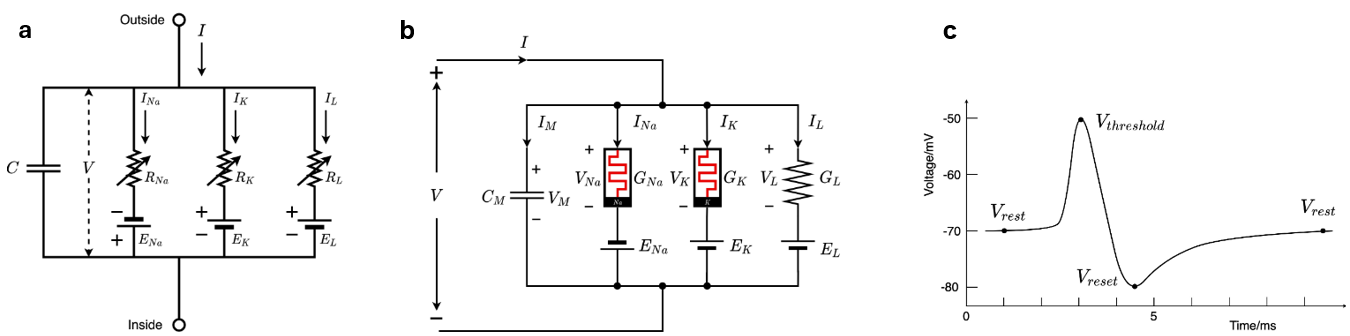
\includegraphics[width=1\textwidth]{Chapter2/Figs/c.png}
    \caption[Hodgkin-Huxley neuron model.]{(a) An equivalent circuit for the Hodgkin-Huxley (HH) models \cite{hodgkin1952quantitative}. (b) An action potential waveform, which demonstrates the resting, threshold, and reset potentials \cite{chua2012hodgkin}.}
    \label{fig:2c}
\end{figure}

% \begin{figure}[htbp!] 
%     \centering    
%     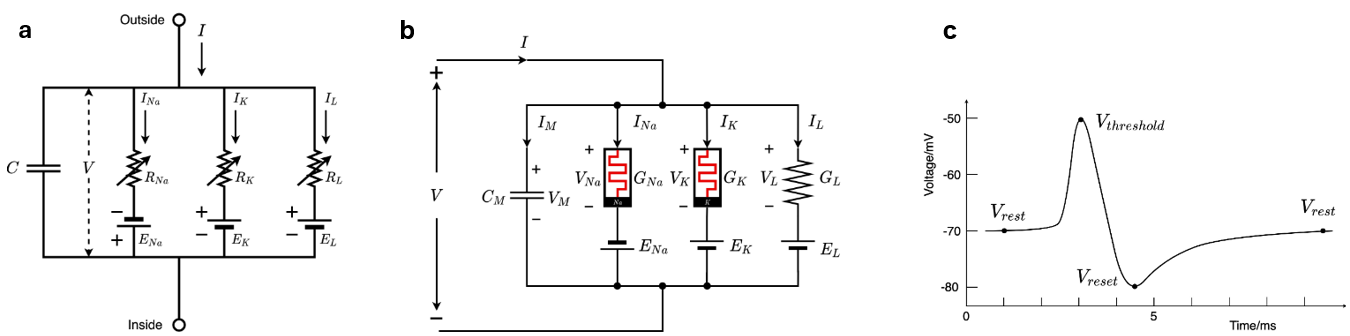
\includegraphics[width=1\textwidth]{Chapter2/Figs/c.png}
%     \caption[Hodgkin-Huxley neuron model.]{Hodgkin-Huxley neuron model. (a) An equivalent circuit for the HH models \cite{hodgkin1952quantitative}. (b) An equivalent circuit for memristive HH model \cite{chua2012hodgkin}. (c) An action potential waveform, which demonstrates the resting, threshold, and reset potentials. }
%     \label{fig:2c}
% \end{figure}

\noindent A significant proportion of the most influential findings in computational neuroscience are based on mathematically detailed models of neuronal functioning. One of the most renowned of these is the Hodgkin-Huxley model of the squid giant axon \cite{hodgkin1952quantitative}. the Hodgkin–Huxley (HH) model is one of the most widely used, comprising a set of nonlinear differential equations that accurately approximate the electrical signals of neurons \cite{chua2012hodgkin}. \\

\noindent Figure \ref{fig:2c}(a) depicts the HH neural model, wherein the time-varying nonlinear conductor $R_{Na}(GNa)$ and $R_K(G_K)$ represent the sodium and potassium channels, respectively, while the linear conductor $R_L(G_L)$ simulates leak channels and $C$ models the membrane of a neuron. The equations of the HH model are presented below: 
\begin{align}
    C \frac{dV_m(t)}{dt} = I_C(t) + \sum_{k}^{}I_k(t) \label{eq:2.1} 
\end{align}

\noindent In this context, $V_m$ represents the membrane potential. $\sum_{k}^{}I_k(t)$ denotes the sum of the ionic currents flowing into the neuron. This can be formulated by three ion currents, as follows:
\begin{align}
    \sum_{k}^{}I_k &= C_m \frac{dV_m}{dt} + G_Kn^4(V_m - V_K) + G_{Na}m^3(V_m - V_{Na}) + G_L (V_m - V_L) \label{eq:2.2} \\
    \frac{dn}{dt} &= \alpha_n(V_m)(1-n)-\beta_n(V_m)n \label{eq:2.3} \\
    \frac{dm}{dt} &= \alpha_m(V_m)(1-m) - \beta_m(V_m)m \label{eq:2.4} \\
    \frac{dh}{dt} &= \alpha_h(V_m)(1-h)-\beta_h(V_m)h \label{eq:2.5}
\end{align}

\noindent The reversal potentials $V_K$, $V_{Na}$, and $V_L$ are the three parameters in question. The rate constants $\alpha_i$ and $\beta_i$, which depend on the membrane potential, describe the behaviour of the $i^{th}$ ion channel. The maximal value of the conductance is represented by $G_K$, $G_{Na}$, and $G_L$. \\

\noindent Finally, the dimensionless quantities \textit{n}, \textit{m}, and \textit{h}, which lie between 0 and 1, are associated with three ion channels. In order to achieve the optimal fit for human action potentials, the HH model is reduced by setting the leakage channel conductance to $G_L = 0$  \cite{noble1962modification}.It has been demonstrated that $G_{Na}$ and $G_K$ are memristors \cite{chua1976memristive}, in the equivalent circuit in figure \ref{fig:2c}(b). \\

\noindent The integrate-and-fire (IF) neuron \cite{lapicque1907louis} constituted one of the earliest computational models of a neuron. This model was developed prior to the ability of researchers to measure the electrical and chemical changes occurring in a functioning neuron. It is based on the premise that the neuron membrane can be modelled as a capacitor that stores charge over time \cite{abbott1999lapicque}.\\

\noindent As the name suggests, the IF model exhibits two principal behaviours: The model integrates current over time, as would be expected of a capacitor, and fires when the voltage reaches a threshold. Furthermore, the model may or may not incorporate a leak term, which represents a resistor in parallel with the capacitor that permits the dissipation of charge over time. The model with a leak term is typically designated as the leaky integrate-and-fire (LIF) model. While the term "integrate-and-fire (IF) model" can be used interchangably. \\

\noindent To identify how the neuron's membrane voltage evolves over time and, based on this, to determine when the neuron spikes, the charge \textit{Q} across a capacitor is represented by $Q = V \times C$, where \textit{V} is the voltage across the capacitor and \textit{C} is the capacitance. By differentiating this with respect to time, the membrane voltage $\textit{V(t)}$ of the neuron is:
\begin{align}
    C \frac{dV(t)}{dt} = J(t) \label{eq:2.6} 
\end{align}

\noindent In this context, \textit{J(t)} represents the input current to the neuron over time, whereas \textit{C} denotes the membrane capacitance. The current here is the time derivative of charge. Equation \ref{eq:2.6} demonstrates that the IF neuron simply integrates the input current over time. It is still necessary to identify the point at which the neuron spikes. \\

\noindent This is achieved by defining a threshold voltage, $V_{th}$, which is exceeded when the voltage passes this threshold, resulting in the neuron firing. This is a fundamental principle in neurophysiology: once the neuron voltage passes a threshold, the neuron begins firing a spike, and once this firing process begins, it is almost impossible to reverse. \\

\noindent Once a neuron has fired a spike, the membrane voltage is reset to the resting potential, $V_{rest}$. This phenomenon can be attributed to physiological resetting procedures. Following the occurrence of a spike in a neuron, other ionic currents, typically potassium, are initiated, leading to a restoration of the membrane voltage towards the resting potential.\\

% \noindent Some integrate-and-fire models may also incorporate an absolute refractory period, defined as a time interval during which the voltage is maintained at the resting potential $V_{rest}$ following a spike. In cortical neurons, post-spike potassium currents are sufficiently strong to prevent another spike from occurring for a considerable duration. This time interval is referred to as the absolute refractory period. The model accounts for this by holding the membrane voltage at $V_{rest}$ for a duration equal to the absolute refractory period. \\

\noindent The leaky integrate-and-fire (LIF) model \cite{knight1972dynamics} incorporates an additional physiological factor: Neuron membranes are not perfect capacitors; rather, they slowly leak current over time, pulling the membrane voltage back to its resting potential. Therefore, the membrane is modelled as a capacitor and resistor in parallel, which allows for the neuron to exhibit a degree of "forgetting": in the absence of any input, the membrane voltage will return to its resting potential \cite{koch2004biophysics}. The LIF dynamics are captured by the following equation:

\begin{align}
C \frac{dV(t)}{dt} = J(t) - \frac{1}{R} (V - V_{rest}) \label{eq:2.7} 
\end{align}

\noindent In this model, \textit{R} represents the membrane resistance, and the remaining parameters are consistent with those of the IF model, with identical resetting procedure.\\

\noindent The LIF model comprises a number of parameters, including $C, R, V_{rest}$ and $V_{th}$. It is possible to normalise the model in order to reduce the number of parameters while maintaining the full dynamics of the original model. In particular, the model can be manipulated so that the normalised voltage lies within the range [0, 1], with a normalised resting potential of zero and a normalised firing threshold of one. Initially, Equation \ref{eq:2.7} is multiplied by R to give:

\begin{align}
    \tau_{rc} \frac{dV}{dt} &= RJ(t) - V + V_{rest} \label{eq:2.8} \\
    \tau_{rc} &= R \times C \label{eq:2.9} \\
    \bar{V} &= \frac{V - V_{rest}}{V_{th} - V_{rest}} \label{eq:2.10} \\
    \bar{V_{rest}} &= \frac{V_{rest}}{V_{th}} \label{eq:2.11} 
\end{align}

\noindent By substituting $\bar{V}$ and $\bar{V_{rest}}$ into equation \ref{eq:2.3} to give:


\begin{align}
    \tau_{RC}(V_{th} - V_{rest})\frac{d\bar{V}}{dt} &= RJ(t) - \bar{V}(V_{th} - V_{rest})
    \label{eq:2.12} \\
    \tau_{rc}\frac{d\bar{V}}{dt} &= \frac{R}{V_{th} - V_{rest}} J(t) - \bar{V} \label{eq:2.13} \\
    \tau_{rc} \frac{d\bar{V}}{dt} &= \bar{J}(t) - \bar{V} \label{eq:2.14} 
\end{align}

\noindent When the firing threshold for the new equation $\bar{V_{th}} = 1$, the voltage resets to $\bar{V_{rest}} = 0$, and $\bar{J}(t) = \frac{R}{V_{th} - V_{rest}} J(t)$. It can be observed that $\bar{J}(t)$ is merely a linear transformation of $J(t)$. Consequently, (\ref{eq:2.14}) retains the full dynamics of (\ref{eq:2.7}) for a scaled input, but with only one parameter, $\tau_{RC}$. \\

\noindent It should be noted that both $\bar{V}$ and $\bar{J}$ are unitless quantities. Conventionally, the unitless space is employed exclusively, and the quantities are often referred to simply as \textit{V} and \textit{J}, despite the fact that they are not voltages or currents. This simplifies the mathematical representation, without limiting the generality of the models. \\

\noindent (\ref{eq:2.14}) provides an exact description of the circumstances under which the model neuron will spike in response to a given input current, \textit{J(t)}. However, in some cases, it is sufficient to consider only the spike rate, that is, the number of spikes per second that the neuron will produce in response to a given input current. \\

\noindent In the case of the LIF model, it is possible to determine the analytical firing rate for a constant input current. This is achieved by calculating the inter-spike interval (ISI), which is the time between one spike and the next. The firing rate is then given by the inverse of the ISI. When a constant input current, $J(t) = j$, is provided, it is possible to solve (\ref{eq:2.14}) in order to find the neuron voltage over time. 
\begin{align}
    V(t) = (V(0) - j)e^{\frac{-t}{\tau_{rc}}} + j \label{eq:2.15}
\end{align}

\noindent In the absence of spikes, the objective is to ascertain the time required for the voltage to increase from$ V(0) = 0$ to $V(t) = 1$. This property will only occur if $j > 1$. Substitution into (\ref{eq:2.15}) and subsequent solution for \textit{t} yields:
\begin{align}
    t = - \tau_{RC} log \left( - \frac{1}{j} \right) \label{eq:2.16}
\end{align}

\noindent Incorporating the refractory period and performing the inversion, the spike rate \textit{r} for the LIF neuron is given by:
\begin{align}
    r &= \begin{cases}
    \frac{1}{t_{ref} - \tau_{RC} log \left( 1 - \frac{1}{j} \right)} & \text{ if } j > 1 \\ 
    0 & \text{ otherwise }  
    \end{cases} \label{eq:2.17}
\end{align}


\noindent The LIF model is one of the most widely utilised simplified neuron models \cite{lapique1907researches}. The simple equivalent model is illustrated in Figure \ref{fig:2d}(a). In this model \cite{stein1967frequency}, a resistor \textit{R}, connected in series with a \textit{DC} source $V_{rest}/V_{reset}$, is connected in parallel with a capacitor \textit{C}. A postsynaptic neuron receives a synaptic current \textit{I(t)}, generated by presynaptic spikes. \\

\noindent A proportion of the current \textit{I(t)} flowing into \textit{C} results in an increase in the membrane potential \textit{V(t)}. The charge leakage occurs via resistor \textit{R}. When \textit{V(t)} reaches a threshold value, the neuron generates a spike. Following the generation of a spike, the membrane potential is reset to the reset value. \\

% \begin{figure}[htbp!] 
%     \centering    
%     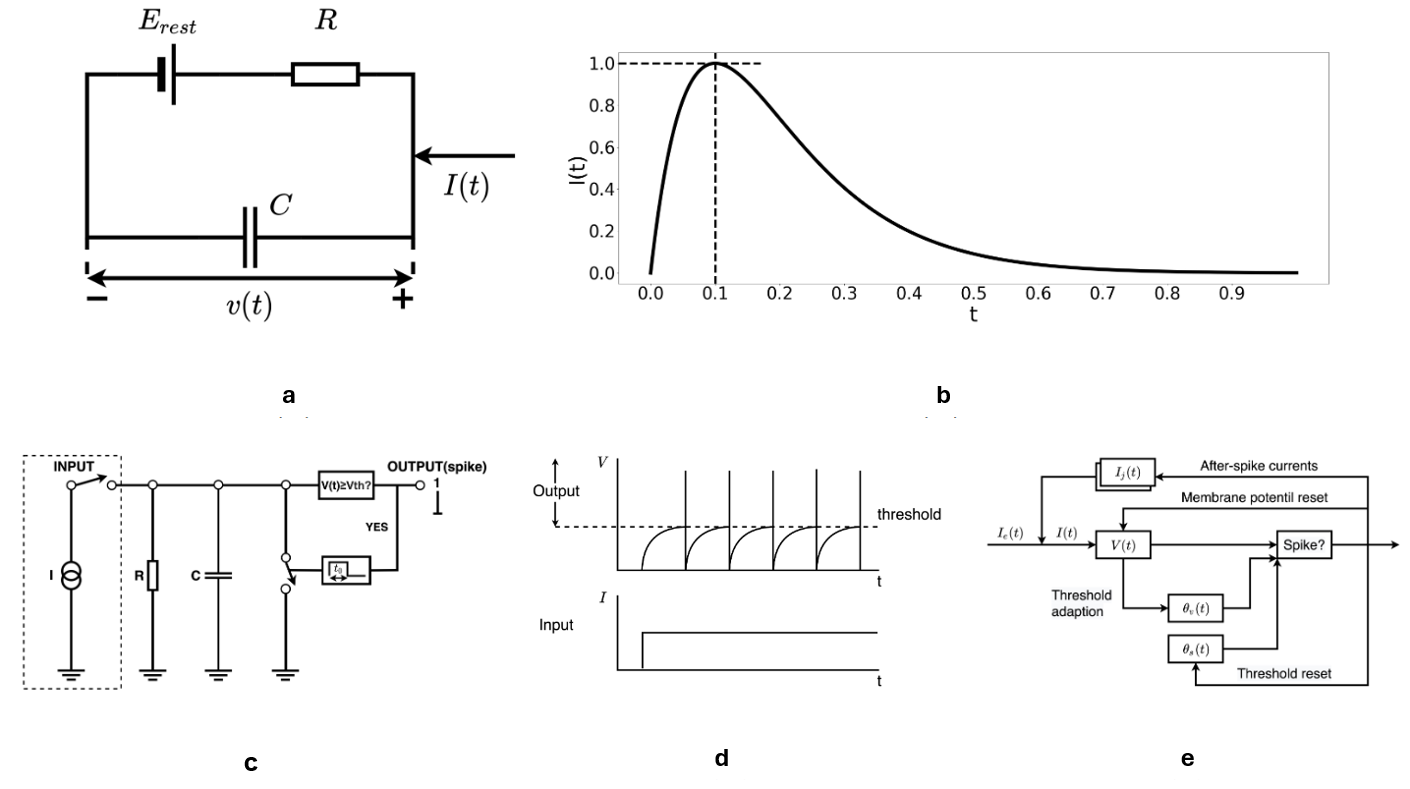
\includegraphics[width=0.8\textwidth]{Chapter2/Figs/d.png}
%     \caption[The Leaky Integrate-and-Fire neuron model.]{The LIF neuron model. (a) Schematic diagram of the LIF electrical model. (b) Input current in the form of an alpha function, $\tau_{\alpha} = 0.1, I_0 = 1$ (c) The LIF model allows for the control of spiking behaviour through a comparison of membrane potential and threshold at each time step. Upon the triggering of a spike, a voltage-controlled switch discharges C for a duration corresponding to the refractory period $t_0$ \cite{tal1997computing}. (d) A simulation of constant firing frequency for DC current input in which $t_0$ is hidden. DC input current and output spikes are both shown. (e) A generalised LIF model with threshold control \cite{teeter2018generalized}. }
%     \label{fig:2d}
% \end{figure}

\begin{figure}[htbp!] 
    \centering    
    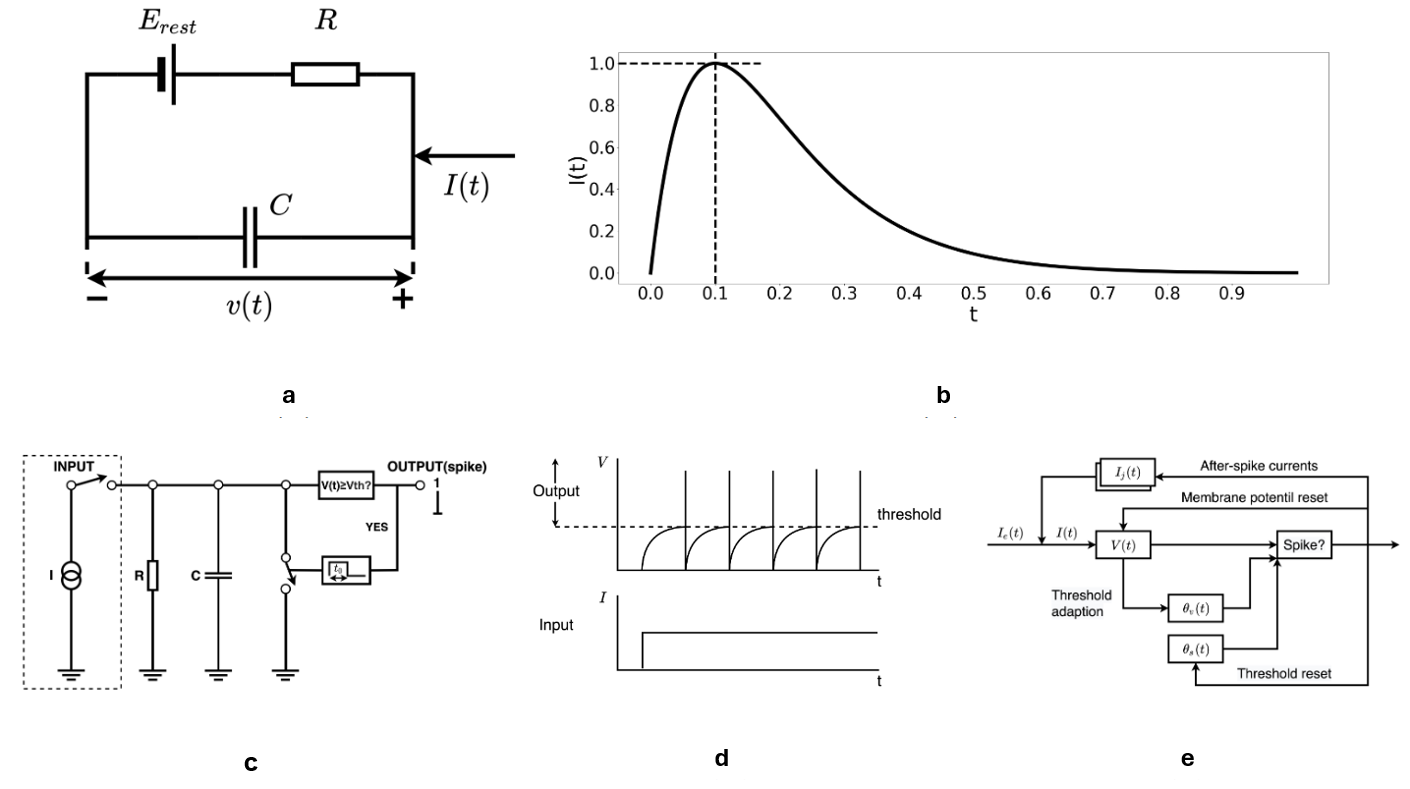
\includegraphics[width=1\textwidth]{Chapter2/Figs/d.png}
    \caption[The Leaky Integrate-and-Fire neuron model.]{(a) Schematic diagram of the LIF electrical model. The LIF model allows for the control of spiking behaviour through a comparison of membrane potential and threshold at each time step. Upon the triggering of a spike, a voltage-controlled switch discharges C for a duration corresponding to the refractory period $t_0$ \cite{tal1997computing}. (b) Input current in the form of an alpha function \cite{teeter2018generalized}.}
    \label{fig:2d}
\end{figure}

\noindent In the absence of \textit{I(t)}, the voltage across \textit{C} is eventually settled at $V_{rest}$, representing the cell's resting potential. During the refractory period $t_0$, a neuron is incapable of spiking. Figure \ref{fig:2d}(c,d) illustrates the LIF neuron dynamics for the case of a \textit{DC} input current and a zero rest and reset potential, $E_{reset} = E_{rest} = 0$ \cite{tal1997computing}. \\

\noindent The input synaptic current, \textit{I(t)}, can be described by a time-varying alpha function. However, alternative functions may be employed, including "Instantaneous Rise and Single Exponential Decay," "Biexponential Functions," "Sawtooth," and "Pulse Function." The alpha synaptic current is modeled by Equation \ref{eq:2.15}, and the resulting plot is shown in Figure \ref{fig:2b}(b). \\

% \noindent Nevertheless, Figure \ref{fig:2d}(a) lacks a circuit for resetting the system when the threshold is reached. In order to evaluate the inequality $V > V_{threshold}$, it is necessary to use an active circuit, such as a comparator. Upon reaching the threshold, the membrane potential must be reset in accordance with the illustration in Figure \ref{fig:2d}(d). Therefore, the LIF model's generalized version necessitates additional overhead, as illustrated in Figure \ref{fig:2d}(e). \\



% \noindent In the generalized LIF model, the reset behavior necessitates external control to pull down the membrane potential below the resting potential. This external control requires intricate, active circuits comprising MOS transistors, resistors, and even a silicon-controlled rectifier (SCR), which represents a significant drawback in a neuromorphic system due to its substantial power and area consumption. \\

% \noindent In order to address the limitations of conventional neuron models, memristor technologies can be employed to emulate biological neurons with the objective of reducing energy consumption and increasing packing density. The HH model has been emulated by utilising two memristors in parallel with two capacitors, respectively mimicking two channels that are coupled to each other with a resistor. \\

% \noindent Additionally, an input resistor and an output impedance comprising a resistor and a capacitor have been proposed \cite{pickett2013scalable}. The LIF neuron has been demonstrated using a diffusive/volatile memristor in parallel with a capacitor, and the neuron has been employed in a fully memristive neural network \cite{wang2018fully}. \\

% \noindent Despite the existence of memristor-based neuron models, the lack of accessible experimental data and hardware for prototyping memristive circuits represents a significant obstacle. A significant number of state-of-the-art experimental demonstrations have relied on bespoke fabrication processes that cannot be reproduced using off-the-shelf memristors. \\

% \noindent Furthermore, the limited choice of commercially available, low-cost, discretely packaged memristors, which are known to be highly sensitive and stochastic in behaviour, has compounded the issue. The challenge in developing hardware prototypes has made it difficult to perform experimental validation. \\

% \noindent In addition to the acceleration of neural networks, the design of a solid-state brain that can harness the neural code has gained increasing attention as a means of processing vast quantities of sensory data without being constrained by the von Neumann bottleneck. The solid-state brain is structured in a manner that emulates the cerebral cortex, with neurons interconnected by a vast array of variable synapses. \\

% \noindent It is hypothesised that neurons and synapses can be realised with memristors integrated with a complementary metal-oxide semiconductor (CMOS) process. However, the design of a large-scale solid-state brain remains elusive in neuromorphic computing due to the considerable overheads associated with mimicking the surface area of neural tissue, constrained power consumption, routing, and the massive parallelism of synaptic connections.

\noindent It is evident that neurons manifest considerable heterogeneity with regard to their dynamics, morphology and connectivity. They can summarily be categorised as follows: Excitatory neurons are responsible for promoting activity in connected neurons. In contrast, inhibitory neurons are responsible for suppressing activity, a process that is crucial for stability and rhythm. Finally, interneurons connect local circuits, thereby enabling complex computations.

\subsection[Synaptic Transmission and Plasticity]{Synaptic Transmission and Plasticity}

Prior to model internal neural dynamics, it is essential to model the dynamics of the synapses that connect neurons to one another. Synapses exert a significant functional effect as a low-pass filter on the spikes that pass through them. A spike in the presynaptic neuron elicits an extended current pulse in the postsynaptic neuron. This pulse can be conceptualised as a low-pass filtered version of the presynaptic spike. \\

\noindent The simplest model of a synapse is that of a first-order low-pass filter. The impulse response of a filter describes the manner in which the filter responds to an infinitesimally short input of unit integral, which is called an impulse. This idealised impulse is also a reasonable model of a spike, and thus the impulse response also describes what the postsynaptic current will look like in response to a presynaptic spike. The impulse response of the first-order low-pass filter is as follows:
\begin{align}
h(t) = \frac{1}{\tau_s}e^{\frac{t}{\tau_s}} \label{eq:2.18} 
\end{align}

\noindent The synaptic time constant, denoted by $\tau_s$, is defined as the length of time over which the postsynaptic current is spread. Given that the impulse response is an exponential function, the exponential synapse model is therefore a suitable description.
\begin{align}
h(t) = \frac{1}{\tau_s^2}e^{\frac{t}{\tau_s}} \label{eq:2.19} 
\end{align}

\noindent It was determined that a second-order lowpass filter is a superior model for a synapse \cite{mainen1995reliability}. The impulse response of this filter is defined by (\ref{eq:2.19}). This function is referred to as the alpha function, and thus the model is designated as the alpha synapse model. Both of these models are based on the current generated by a spike in the postsynaptic neuron, which is a current-based synapse model.\\

% \noindent Other current-based synapse models exist; a popular one is the double-exponential model, which is similar to the alpha synapse but with two time constants, thereby affording greater control over the rise and fall of the impulse response. Where The double-exponential model with both time constants set to the same value reduces to the alpha synapse. \\

% \noindent Many of the other, more realistic synapse models are conductance-based, meaning that they model the conductance of the neural membrane at the synapse. The current flowing into the neuron is dependent on both the conductance and the voltage across the membrane. The latter undergoes a change as the synapse becomes active. \\

% % \subsection[Neural Coding Schemes]{Neural Coding Schemes}

\noindent One of the primary objectives of computational neuroscience is to ascertain the manner in which the brain represents—or encodes—information. To this end, researchers have put forth a multitude of potential coding schemes that neurons could utilise for information encoding. One key distinction between rate coding and temporal coding is the following dichotomy. \\

\noindent In a rate code, the sole pertinent measure is the firing rate (i.e. the number of spikes) of a neuron over a given period of time. An exemple of a rate code is motor neurons in the peripheral nervous system. The contraction of a muscle is contingent upon the number of spikes per unit time; thus, only the rate of motor neuron spikes is significant \cite{gerstner1997neural}. In a temporal code, the time of individual spikes is also a factor. For example, in the early auditory system, precise spike timing facilitates the localisation of sounds \cite{chase2006spike}.\\

\noindent The precise definitions of rate and temporal codes remain contentious, with differing interpretations presented by various authors \cite{dayan2005theoretical}. To illustrate, a neuron may discharge a number of spikes in rapid succession, followed by a period of quiescence. A second neuron may be observed to fire the same number of spikes, but in a more evenly distributed manner over a given period. \\

% \noindent One possible interpretation is that both neurons have the same firing rate, but the first has all its spikes occurring near the beginning of the period, in which case the timing of the spikes is a significant factor. An alternative perspective posits that the instantaneous firing rate of the first neuron fluctuates over the period, whereas that of the second neuron remains constant. This suggests that it is the instantaneous firing rate, rather than the overall firing rate, that is of primary importance. \\

% \noindent This highlights a limitation of solely examining the overall firing rate (i.e., the number of spikes) of a neuron over a given period. It is unclear which period should be considered. In real neurons, the period of time that is relevant for counting spikes depends on parameters such as the membrane time constant tau of the postsynaptic neuron. \\

% \noindent For this reason, neuroscientists will often differentiate between rate and timing codes based on the frequency of alterations in the instantaneous firing rate. If the rate of firing exhibits rapid fluctuations, and if these fluctuations contain information about the stimulus (and are not simply spurious variation or "noise"), then the code is said to be temporal; otherwise, it is a rate code. \\

% \noindent Once again, there is a lack of consensus regarding the minimum frequency of fluctuations in firing rates that must be observed to qualify as temporal codes. One possible definition is relative to the stimulus. The firing rate of neurons can be triggered to change rapidly in response to fast-changing stimuli, regardless of whether the code in use is rate or temporal. \\

% \noindent If the temporal code is defined as having meaningful firing rate fluctuations at a faster time scale than changes in the stimulus, then it can be differentiated between codes that have fluctuations because they are using them for coding and those that simply have fluctuations triggered by the stimulus. According to this definition, neurons using a temporal code will have a fluctuating firing rate in response to a constant stimulus, whereas neurons using a rate code will have a non-fluctuating firing rate. \\

\noindent Both rate codes and temporal codes describe the encoding properties of individual neurons. Additionally, one may inquire about the coding properties of a group (also known as a population) of neurons. The concept of population coding pertains to instances where a representation is distributed across numerous neurons within a population, such that the represented value cannot be decoded from the activities of a limited number of neurons.\\

\noindent The simplest method of extrapolating the concept of rate or temporal coding to multiple neurons would be to have numerous neurons all implementing the same code. In other words, all neurons will exhibit a similar firing pattern when representing a given value, due to their comparable tuning properties. This results in a significant degree of redundancy between neurons. \\

\noindent In contrast, population coding entails each neuron representing a distinct aspect of the represented value. To illustrate, if the objective is to represent head direction, there are neurons that represent a head that is fully turned to the left, others that represent a head that is fully turned to the right, and still others that represent a centred head. Additionally, there are neurons that represent values in between these three head directions. The direction in which a neuron is most active is referred to as its preferred direction. \\

% \noindent It should be noted that each neuron exhibits some degree of variance, whereby it will fire for head directions that are relatively close to its preferred direction. Conversely, the further the actual head direction is from a neuron's preferred direction, the less it will fire. By utilising the activities of all neurons in the population, it is possible to decode the head direction with a high degree of accuracy. \\

% \noindent From a population perspective, it is possible to differentiate between codes that exploit synchrony between neurons and those that do not. This can be facilitated, for example, by coincidence detection, whereby a postsynaptic neuron will only fire if the spikes of two of its input neurons are coincident, that is to say, they fall within the same (small) temporal window. \\

% \noindent This distinction between temporal and rate coding schemes is further exemplified by the fact that only temporal codes can take advantage of correlations between individual spikes of neurons. Rate coding schemes, on the other hand, can only take advantage of synchrony between neurons in terms of synchronised fluctuations of their instantaneous firing rates, since they lack the temporal precision to co-ordinate individual spikes.

\noindent Synapses are therefore known to play a dual role in the nervous system. They facilitate communication between neurons and serve as the primary locus of learning and memory. The magnitude of this influence, or 'synaptic strength' \cite{bastos2022motor}, is determined by the relative strength of the connection between the presynaptic and postsynaptic neurons. This phenomenon is known as synaptic plasticity. \\

\noindent It is important to note that plasticity can be categorised into several distinct types. Short-Term Plasticity (STP): Transient changes that last from milliseconds to seconds. Long-Term Potentiation (LTP) and Long-Term Depression (LTD): The phenomenon of sustained increases or decreases in synaptic strength over time. \\

\noindent The most significant model of synaptic plasticity is Hebbian learning, which can be succinctly summarised as follows: The hypothesis that neurons that fire together wire together has been proven to be accurate. A more precise, temporally-sensitive rule is Spike-Timing Dependent Plasticity (STDP) \cite{zheng2018learning}. \\

\noindent Mathematical Models can capture the effect of precise spike timing on synaptic weight updates. If a presynaptic neuron fires before a postsynaptic neuron within a short window, the synapse is strengthened; if the order is reversed, the synapse weakens. A common representation for this is:
\begin{align}
\Delta w = \left\{ \begin{array}{cl}
    A_+ \cdot e^{-\Delta t/\tau_+}, & \ \Delta t > 0 \\
    -A_- \cdot e^{-\Delta t/\tau_-}, & \ \Delta t < 0
    \end{array} \right. \label{eq:2.20}
\end{align}

\noindent Where $\Delta t = t_{post} - t_{pre}$ is the timing difference, $A_+, A_-$ are learning rates, $\tau_+, \tau_-$ are time constants for potentiation and depression. This asymmetric window is indicative of experimental observations and provides a biologically plausible basis for synaptic learning in hardware.\\

\noindent As a small primer, memristive devices offer an electronic analogue to synapses due to their tunable conductance and memory of past activity. When configured in crossbar arrays, these devices have the capacity to implement synaptic weight matrices directly in hardware, with updates governed by local voltage or current pulses.\\

\noindent Memristive STDP implementations frequently exploit device physics, where conductance change is contingent on pulse overlap:
\begin{align}
    \Delta G = f(V_{pre}, V_{post}, \Delta t) \label{eq:2.21}
\end{align}
\noindent where $f$ is a device-specific function determined by material properties and pulse shapes. \\

\noindent It is important to note that memristors have the capacity to inherently facilitate the nonlinear, history-dependent behaviour that is characteristic of biological plasticity rules, such as STDP. To illustrate this point, the application of carefully timed voltage pulses to a memristor has been demonstrated to result in an increase or decrease in conductance, respectively, reminiscent of LTP and LTD.

\section[Foundations of Neuromorphic Computing]{Foundations of Neuromorphic Computing}

Extensive research has been conducted in device physics and material science to explore innovative materials and techniques for memories and prolonged retention objectives \cite{indiveri2021introducing}. The term "neuromorphic" was created by researchers to describe new technologies and systems that, in addition to being essential for the construction of massive AI computer networks, exhibit certain behaviours that can be compared to those of real synapses \cite{di2009circuit}. \\

\noindent Soon after, the notion of using these novel nanoscale components as "memristors" gained popularity, with the underlying notion being that they could be utilised to produce synapses in deep neural networks and sustain their synaptic weights locally \cite{jo2010nanoscale}. The hardware and technology described could enable neural networks to perform "in-memory computing" and exhibit advanced non-linear properties, mimicking the physics of biological synapses \cite{saighi2015plasticity}. \\

\noindent The research in this field aims to develop various types of volatile and non-volatile memristive electronics. Additionally, spike or pulse-based control systems are being created to elicit biologically realistic learning behaviours in memristive cross-bar arrays. The challenging task is to find the perfect artificial synapse, which requires investigation into different materials, tools, and techniques.

\subsection[Memristor Fundamentals]{Memristor Fundamentals}

Memristive devices, also known as memory resistors, are emerging as foundational elements in neuromorphic computing due to their ability to retain resistive states based on electrical history, thereby emulating biological synapses. The central purpose of these components is to facilitate both memory storage and computation within a unified, compact structure, thereby enabling the co-location of memory and processing elements that is vital for brain-inspired architectures.\\

\noindent The presence of symmetry in nature, which is believed to arise from a common origin, is remarkable.  However, the traditional electromagnetic passive circuit components of resistor, capacitor, and inductor are inadequate for describing the characteristics connected by the symmetry of circuit theory. Leon Chua addressed this issue by introducing the concept of a memristor in 1971 \cite{chua1971memristor}, which couples flux linkage and charge as a circuit device:
\begin{align}
    M(q) = \frac{d\phi}{dq} \label{eq:2.22}
\end{align}

\noindent where $M$ denotes the memristance, a quantity whose value is known to be dependent on the history of the current that has previously passed through the device. This phenomenon gives rise to a form of resistive memory, wherein the device retains a memory of its previous state. However, proof of resistive switching in the memristor model was not established until 2008 \cite{strukov2008missing}.

\begin{figure}[htbp!] 
    \centering    
    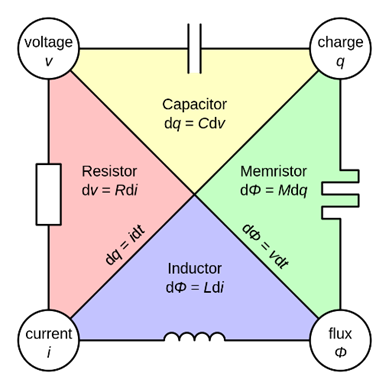
\includegraphics[width=0.5\textwidth]{Chapter2/Figs/e.png}
    \caption[Conceptual symmetries of resistor, capacitor, inductor, and memristor]{Conceptual symmetries of resistor, capacitor, inductor, and memristor \cite{du2017metal}. These four fundamental variables in circuit theory are depicted with their relationships. Each variable can be related to another via either a passive component or a well-known equation.}
    \label{fig:2e}
\end{figure}

\noindent There are three fundamental circuit elements and four essential circuit variables in basic electrical circuit theory.  It is evident that one component is absent to achieve symmetry. This device ought to function in such a way that charge and magnetic flux are interconnected, as illustrated in Figure \ref{fig:2e}. The link between the mathematical memristive model and a two-terminal resistive switching device is pivotal in this instance. \\

\noindent The concept of memristance is distinct from that of resistance in that it is dependent on charge, rather than being a constant value.  The current is defined as the amount of charge flowing per unit time. Therefore, the expression for current can be written as:
\begin{align}
    q = \int_{-\infty}^{t_0} i(t)dt \label{eq:2.23}
\end{align}

\noindent where charge is the sum of current at a given time $t_0$.  \\

\noindent This indicates that the memristance, being dependent on charge, is determined by the historical currents that have previously passed through the device. In the event of interruption to the current flowing through the device, the memory state persists until the current flow is restored. The device is evidently equipped with a type of memory known as a "memristor".\\

\noindent In physical terms, memristors are often modeled as two-terminal devices whose resistance varies due to the drift of ions or vacancies in a dielectric medium. The state-dependent resistance can be written as:
\begin{align}
    V(t) = R(w(t)) \cdot I(t) \label{eq:2.24}
\end{align}

\noindent where $V(t)$ and $I(t)$ are the voltage and current at time $t$, $R(w(t))$ is the resistance depending on the internal state $w(t)$. This state $w(t)$ often represents physical quantities like oxygen vacancy concentration or filament length in resistive switching materials. $f(w, I) = \frac{dw}{dt}$ can be further defined as to how the internal state changes with input current. \\

\begin{figure}[htbp!] 
    \centering    
    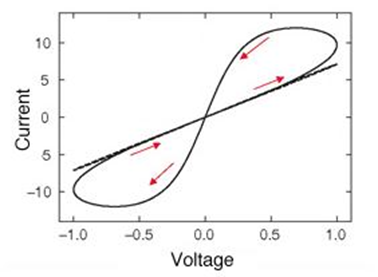
\includegraphics[width=0.5\textwidth]{Chapter2/Figs/f.png}
    \caption[Typical I-V characteristic of a memristor]{The typical I-V characteristic  of a memristor displays a pinched hysteresis loop resulting from the nonlinear relationship between current and voltage in memristance \cite{wen2012dynamics}.}
    \label{fig:2f}
\end{figure}
    
\noindent From a visual standpoint, the pinched hysteresis loop, which is characteristic of the devices and dependent on frequency, distinguishes these memristor devices from other components \cite{chua2019resistance}, as shown in Figure \ref{fig:2f}. This loop represents a prevalent and inherent phenomenon in the natural world. It is evident that as the voltage input frequency increases, the loop undergoes a reduction in size. When the frequency approaches infinity, the memristor can be approximated as a resistor.\\

\noindent Among the range of new non-volatile memory devices, the primary focus of this study is on memristor devices, including MRAM, PRAM, FeRAM, and RRAM \cite{wang2017memristors}. Resistive switching, a reversible phenomenon of two-terminal elements, characterises the devices. Through electrical signalling, they change resistance in a non-volatile manner, with the process driving the resistive switching defined by the device's materials \cite{mehonic2018silicon}. \\

\noindent Resistive random-access memory (RRAM) is a device that uses resistance switching, where reversibility is attained through repeated application of appropriate stimuli, according to \cite{liu2010controllable}. Repeated application of suitable stimuli ensures reversibility. An RRAM cell comprises an insulating thin film (usually a metal oxide), sandwiched between two electrodes, within which resistance switching occurs. \\

\noindent The term "memristance" is favoured to express the general characteristics of these RRAM devices. The central hypothesis of this model is that memristance is a function of the total charge that has been passed through the device or that the integral of the applied voltage is consistent with certain experimental data. This can be used to toggle between different resistance levels. Although this ideal memristor model is often used in RRAM cells, it may not satisfy practical requirements. \\

\begin{figure}[htbp!] 
    \centering    
    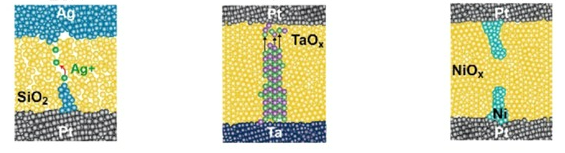
\includegraphics[width=0.8\textwidth]{Chapter2/Figs/g.png}
    \caption[The main RRAM types.]{The main RRAM types, from left to right: electrochemical metallization memory (ECM), vacancy change memory (VCM), and thermochemical memory (TCM). \cite{goux2016electrochemical}}
    \label{fig:2g}
\end{figure} 

\noindent Although all RRAM devices operate on a metal-insulator-metal (MIM) architecture, their categorisation and analysis remain challenging. RRAM devices are loosely classified into two types based on their functional mechanisms: oxide-RAM (OxRAM) and conductive bridge RAM (CBRAM) \cite{liu2015categorization}. \\

\noindent However, the internal physical behaviour of RRAM devices greatly varies, making it difficult to obtain a unified picture of them. RRAM cells may be classified according to their switching mechanisms which are electrochemical metallisation (ECM), valence change mechanism (VCM), or thermochemical mechanism (TCM) \cite{goux2016electrochemical}. The operation of the device is explained by one of the mechanisms depicted in Figure \ref{fig:2g}. \\

\noindent In normal operation, the state of the memristor can be objectively designated as having high resistance in the "OFF" state and low resistance in the "ON" state, with a substantial difference in resistance levels. The shift from the high resistance state (HRS) to the low resistance state (LRS) is referred to as "Set," while the reverse is called "Reset." An electroforming step is generally necessary to convert the device from pristine to switchable, whereby the former tends to exhibit higher resistance. \\

\noindent A hallmark of biorealistic learning is the ability to adjust synaptic strength continuously over time in response to neural activity. Analog (or gradual) switching in memristors is thus essential. Instead of binary ON/OFF transitions, these devices exhibit incremental conductance changes under controlled voltage pulse conditions. Consider a simplified state evolution model:
\begin{align}
    \frac{dw}{dt} = \mu \cdot I(t) \label{eq:2.25}
\end{align}
Where $\mu$ is a mobility parameter dependent on the device materials and structure. For voltage pulses of controlled amplitude and duration, this allows precise modulation of conductance:
\begin{align}
    \Delta G \varpropto \int I(t) dt = Q \label{eq:2.26}
\end{align}

\noindent Here, $Q$ is the total charge transferred, which accumulates over spike events. By shaping input pulses (in terms of rise time, width, or height), one can encode temporally-dependent plasticity rules such as STDP directly in hardware.\\

\noindent Despite their initial promise, memristive devices have been found to exhibit significant non-idealities \cite{govoreanu2013vacancy}. Device-to-device variability, encompassing factors such as conductance range, switching thresholds, and cycle-to-cycle behaviour, has the potential to vary across devices that appear to be nominally identical.\\

\noindent Non-linear phenomena, such as conductance updates, frequently exhibit saturation or asymmetric responses to positive and negative pulses. It is important to note that drift and retention loss, such as those occurring over time, may be attributable to the effects of relaxation. \\

\noindent To address these issues, neuromorphic systems often employ redundancy, error-tolerant learning algorithms, or closed-loop calibration techniques. Furthermore, some variability may be biologically realistic: synapses in the brain are not perfectly precise either, and stochasticity can enhance learning generalization and robustness.\\

\noindent For design and testing purposes, compact models of memristive devices are essential. These range from physics-based models to empirical abstractions. A popular framework is the linear ion drift model \cite{cai2011abel}, applicable to early $TiO_2$-based devices:
\begin{align}
    w(t) = w_0 + \frac{\mu_vR_{ON}}{D} \cdot \int_{0}^{t} I(\tau)   \,d\tau  \label{eq:2.27}
\end{align}

\noindent Where $\mu_v$ is the ion mobility, $R_{ON}$ is the low resistance state, $D$ is the device thickness. For practical simulations, window functions are often added to prevent unrealistic values of $w(t)$ outside the physical boundaries. A widely used modified form is:
\begin{align}
    \frac{dw}{dt} = \mu \cdot I(t) \cdot f(w) \label{eq:2.28}
\end{align}

\noindent Where $f(w)$ is a window function such as:
\begin{align}
    f(w) = 1 - (2w - 1)^{2p} \label{eq:2.29}
\end{align}
\noindent with $p$ controlling the non-linearity near the boundaries. These models allow researchers to prototype neuromorphic algorithms and circuits in software before hardware realization, enabling design-space exploration and validation under realistic conditions.


\subsection[In-memory Computing Paradigms]{In-memory Computing Paradigms}

\noindent Neuromorphic computing signifies a paradigm shift of the manner in which information is processed and stored; this is inspired directly by the architecture and function of biological neural systems. Conventional computing systems compartmentalise memory and processing units, a configuration that engenders energy and velocity inefficiencies due to incessant data movement. Neuromorphic systems are designed to co-locate memory and computation by leveraging distributed, parallel architectures that emulate the brain's functionality.\\

\noindent The origin of neuromorphic engineering can be traced to the pioneering work of Carver Mead in the 1980s \cite{mead1989analog}, who proposed using analog electronics to mimic the function of neurons and synapses. Since then, the field has grown to encompass both analog and digital implementations of brain-inspired circuits.\\

\noindent The fundamental principle of neuromorphic computing is the translation of key neurobiological principles into hardware. Event-driven processing is a key feature of neuromorphic circuits, which, like biological neurons, only activate when necessary, thereby significantly reducing power consumption. \\

\noindent As an illustrative example, synapses (which are implemented by resistive memory elements) function as both computational units and memory stores. Neuromorphic systems have been demonstrated to exhibit plasticity and the capacity for real-time, local learning through the utilisation of biologically plausible rules, such as the STDP (synaptic tagging with depolarisation-dependent plasticity) rule. \\

\noindent Neuromorphic architectures can be broadly classified into two categories \cite{ceolini2020hand}. Digital neuromorphic systems are comprised of digital circuits which simulate the behaviour of neurons, i.e. their spiking. Notable examples of this include IBM's TrueNorth and Intel's Loihi. These chips implement large networks of spiking neurons with programmable connectivity and plasticity. Analog/Mixed-Signal Systems have been shown to exhibit a greater degree of similarity to the continuous dynamics of biological neurons and synapses. Memristive arrays frequently fall into this category, offering a physical substrate for analogue computation.\\

\begin{figure}[htbp!] 
    \centering    
    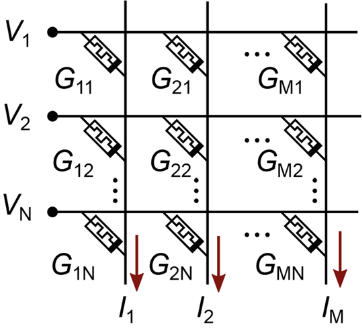
\includegraphics[width=0.5\textwidth]{Chapter2/Figs/h.png}
    \caption[The memristor-based crossbar architecture.]{The memristor-based crossbar architecture with a single memristor array and a constant-term circuit \cite{truong2014new}. The resistive components are located at the connections of the word and bit lines. When voltages $\mathbf{V}$ are applied to the word line, the resistive element at the junction of the $i^{th}$ word line and the $j^{th}$ bit line generates $V_i \times G_{i,j}$ units of current, assuming zero wire resistance, as per Ohm's law. The currents created by each individual element are then aggregated along the bit lines using Kirchhoff's current law.}
    \label{fig:2h}
\end{figure}
    

\noindent A key architectural unit is the crossbar array, in which vertical and horizontal metal lines intersect at memristive devices. This structure supports efficient matrix-vector multiplication—the fundamental operation in neural networks. Let $V$ be a voltage vector applied to input rows, and $G$ be the conductance matrix of memristive elements. The output current vector $I$ on the columns is given by:
\begin{align}
    \mathbf{I} = \mathbf{G} \cdot \mathbf{V} \label{eq:2.30}
\end{align}

\noindent This analog computation occurs in a single step without requiring data movement between separate processing and memory units, thus offering significant energy efficiency. Linear algebra and vector-matrix products rely heavily on multiplication and addition. These procedures can be carried out by using fundamental circuit laws. \\

\noindent Consider a resistive element with conductance $G$ (the reciprocal of resistance). If a voltage $V$ is supplied to it, the current $I$ flowing through it will be equal to $V \times G$. This indicates that conductance $G$ functions as a multiplicative factor, as per Ohm's law. For a circuit with several branches, each carrying a current $I_i$. At the intersection of these branches, the total current flowing through it will be $I = \sum_{i}^{} I_i$. This indicates that currents are combined together, as per Kirchhoff's current law. \\

\noindent Once multiplication and addition are possible, higher-level operations may be performed using specialist circuits. For vector-matrix products, a resistive crossbar array can be used, which is a two-dimensional grid of conductive wires with resistive components at each intersection. A crossbar array's output currents are essentially the product of a voltage vector and a conductance matrix. Consider a vector-matrix product, $\mathbf{y} = \mathbf{x}^\intercal \mathbf{W}$. Where $\mathbf{x}$ can be translated to voltages $\mathbf{V} = k_V\mathbf{x}$, $\mathbf{W}$ to conductances $\mathbf{G} = k_G \mathbf{W}$, and generate outputs $\mathbf{y}$ from currents $\mathbf{I} = \mathbf{y} k_V k_G $, where $k_V$ and $k_G$ are positive constants. \\


\noindent Crossbars can compute products of voltage vectors and conductance matrices due to their structural design. This is because the structure controls which voltage-conductance pairs are multiplied and which consequent currents are combined together. These circuits have two sets of wires: word lines and bit lines. Voltages $\mathbf{V}$ are applied to the word lines, and currents $\mathbf{I}$ are measured along the bit lines. A resistive element located at the junction of the $i^{th}$ word line and the $j^{th}$ bit line has a conductance of $G_{i,j}$.\\
    
\noindent When $V_i$ is applied to the $i^{th}$ word line, the device generates a current of $V_i \times G_{i,j}$ (assuming no wire resistance). The currents generated in the jth bit line are added together to provide a current of $I_j$. This current is calculated by taking the dot product of voltage $\mathbf{V}$ and the $j^{th}$ column of the conductance matrix $\mathbf{G}$. Given that the $j^{th}$ element of a vector-matrix product is just the dot product of the vector and the $j^{th}$ column of the matrix, the vector containing all output currents may be concisely expressed as $\mathbf{I}^\intercal = \mathbf{V}^\intercal \mathbf{G}$. \\
    
\noindent The individual application determines which resistive devices are used in the crossbar array. Weights $\mathbf{W}$ are repeatedly updated during neural network training, necessitating the ability to alter the conductances in the crossbar array numerous times. In contrast, during inference, the weights are fixed, allowing the conductances to be set after initial programming. Regardless of the conditions, the conductances will be unique to the network, requiring the ability to change them at least once. \\
    
\noindent Memristive devices, or memrisitors, are differentiated by their ability to change their conductance in response to electrical inputs. As a result, they make an excellent choice for crossbar-based linear algebra accelerators. The choice of memristor depends on whether the crossbar array is used for training or inference. The former is far more difficult and would demand memristors that can be repeatedly programmed in a linear fashion. Given these complications, much research on memristive crossbars has been on inference. \\
    
\noindent Even in the absence of nonidealities, any memristor will have a restricted range of conductance values that it can be configured to. This is a hurdle when attempting to represent real numbers with solely positive conductances $G$. To demonstrate, if the range of attainable conductances is $G \in [G_{off}, G_{on}]$, the crossbar array can only represent matrix values up to $w \in \left [ \frac{G_{off}}{k_G}, \frac{G_{on}}{k_G} \right ]$. Since $G_{off}$ is a positive number, hence only positive $w$ may be expressed. \\
    
\noindent One potential option is to employ differential pairs, in which the matrix element $w$ is represented as the difference between two conductances, $G+$ and $G-$ \cite{joksas2022nonideality}. The two conductances can be chosen symmetrically around the 'average' value $G \pm = G_{avg} \pm \frac{k_G w}{2}$, where $G_{avg} = \frac{G_{off} + G_{on}}{2}$. The two sets of conductances can be represented by independent conductance matrices $\mathbf{G}+$ and $\mathbf{G}-$, which are assigned to different bit lines of the crossbar array \cite{kim20214k}. \\
    
\noindent The bit lines will then generate independent sets of currents, which may be represented as vectors $\mathbf{I}+$ and $\mathbf{I}-$. Vector-matrix products are linear, thus the result may be calculated by subtracting $\mathbf{I}-$ from $\mathbf{I}+$. In reality, the 'positive' and 'negative' bit lines are frequently arranged near to one another, which helps to mitigate the detrimental effects of line resistance, a significant non-ideality \cite{joksas2020committee}. \\

% \noindent Unlike traditional artificial neural networks (ANNs), which use continuous-valued activations, SNNs operate using discrete spikes, more closely resembling biological neurons. In SNNs, information is encoded not in the magnitude of activation but in the timing and frequency of spikes—a paradigm known as temporal coding. \\

% \noindent The dynamic state of a spiking neuron evolves according to differential equations such as those in the LIF model described in previous section. Networks of such neurons can perform complex computations, including pattern recognition, signal processing, and control tasks.\\

% SNNs are particularly well-suited for implementation on neuromorphic hardware due to their:

% Sparsity: Most neurons are inactive at any given time, reducing energy consumption.

% Locality: Updates and communication occur between neighboring units, minimizing global data traffic.

% Temporal Processing: Inherent ability to handle time-series data and asynchronous signals.

\noindent The learning process in neuromorphic systems can be categorised into three distinct approaches: supervised learning, unsupervised learning, and reinforcement-based learning \cite{stone2019artificial}. Nevertheless, with respect to biorealistic implementation, unsupervised, local learning is most aligned with the biological model. \\

\noindent Biorealistic learning draws upon the empirical laws of synaptic plasticity observed in biological systems. Central among these are Hebbian Learning \cite{kempter1999hebbian} which stated "Neurons that fire together wire together." This principle is often expressed in simplified form as:\\
\begin{align}
    \Delta w_{ij} = \eta \cdot x_i \cdot y_i \label{eq:2.31}
\end{align}

\noindent Where $\Delta w_{ij}$ is the change in synaptic weight between pre-synaptic neuron $i$ and post-synaptic neuron $j$, $x_i$ and $y_i$ are the activity levels of the respective neurons, $\eta$ is the learning rate. \\

\noindent Hebbian learning is predicated on the premise that the strength of a synapse is enhanced by co-activity between pre- and post-synaptic neurons \cite{frenkel2019morphic}. Alternatively, STDP is atemporally-sensitive variant of Hebbian learning, a concept that has already been covered in the preceding section. Homeostatic plasticity is a global mechanism that ensures that overall neural activity remains within functional bounds. This is analogous to metabolic regulation in biology.\\

\noindent These mechanisms are often implemented using local circuit rules. For instance, in memristive implementations of STDP, pulse timing determines the net change in conductance of a memristor. The result is a physical device whose behavior embodies the learning rule itself. In digital systems, learning involves weight updates of the form:
\begin{align}
    w_{ij} \leftarrow w_{ij} + \eta \cdot \delta_j \cdot x_i \label{eq:2.32} 
\end{align}

\noindent Where $w_{ij}$ is the synaptic weight from neuron $i$ to neuron $j$, $\eta$ is the learning rate, $\delta_j$ is the error signal at the output neuron $j$, and $x_i$ is the activation of input neuron $i$. In contrast, memristive learning avoids explicit error backpropagation and instead uses local learning rules where the change in conductance $\Delta G$ depends on spike-timing and voltage:
\begin{align}
    \Delta G \varpropto f(\Delta t_{ij}) \cdot g(V_{pre}, V_{post}) \label{eq:2.33}
\end{align}

\noindent Here, $f(\Delta t_{ij})$ reflects the STDP window and $g(V_{pre}, V_{post})$ models the effect of voltage pulses on device conductance. Memristors thus act as "plastic synapses" whose weights evolve in real time, guided by the temporal correlation of pre- and post-synaptic activity.

\subsection[Encoding Plasticity in Memristors]{Encoding Plasticity in Memristors}

As neuromorphic systems aspire to emulate biological intelligence, the implementation of biorealistic learning—learning mechanisms that faithfully reproduce the behavior of biological synapses and neurons—has become central to the development of memristor-based architectures. This section explores how learning rules inspired by neuroscience, such as spike-timing-dependent plasticity (STDP), Hebbian learning, and homeostatic regulation, can be embedded into memristive networks.\\

\noindent To implement STDP and other plasticity rules in hardware, researchers have developed pulse-pairing schemes that encode spike timing as overlapping voltage pulses applied to memristive synapses. These rules can be implemented physically using the conductance modulation behavior of memristors, which act as artificial synapses \cite{campbell2016pulse}. \\

\noindent For instance, a presynaptic spike instigates a positive voltage pulse, whereas a postsynaptic spike precipitates a negative voltage pulse. The net voltage across the memristor depends on the temporal alignment of these spikes. If the pulses overlap constructively (e.g., pre before post), the net voltage exceeds a potentiation threshold, increasing conductance. If the order is reversed (post before pre), the net voltage may trigger depression. \\

\noindent Let the pulse shape be $V_{pre}(t)$ and $V_{post}(t)$, The effective voltage across the memristor is:
\begin{align}
    V_{mem}(t) = V_{pre}(t) - V_{post}(t) \label{eq:2.34}
\end{align}

\noindent Depending on $ V_{mem}(t)$, the conductance $G(t)$ changes according to a windowed integration rule, often expressed as:
\begin{align}
    \Delta G = \int_{-\infty}^{-\infty} \gamma (V_{mem}(t)) \,dt \label{eq:2.35}
\end{align}
\noindent Where $\gamma(\cdot)$ is a non-linear function mapping voltage to conductance change. \\

\noindent At the network scale, memristive synapses form dense connectivity graphs akin to biological networks. When configured with spiking neurons, the resulting system exhibits emergent learning behavior. A typical learning architecture may include a spiking neural network (SNN) layer of leaky integrate-and-fire (LIF) neurons, memristive crossbar arrays that implement synaptic weights, spike-based learning circuits that detect relative spike timing and apply appropriate pulses.\\

\noindent Mathematically, for a neuron receiving inputs $x_i(t)$ through synapses $G_i(t)$, the membrane potential $V_m$ evolves as:
\begin{align}
    C_m \frac{dV_m}{dt} = -\frac{V_m}{R_m} + \sum_{i} G_i(t) \cdot x_i(t) \label{eq:2.36}
\end{align}

\noindent Where $C_m$ and $R_m$ are are the membrane capacitance and leakage resistance respectively. When $V_m$ exceeds a threshold $V_th$, the neuron spikes and resets. Synaptic updates follow:
\begin{align}
    \Delta G_i(t) = f(\Delta t_i) \cdot Pulse_{pairing}(x_i(t), y(t)) \label{eq:2.37}
\end{align}

\noindent With $f(\Delta t_i)$ as an STDP kernel and $Pulse_{pairing}$ as the hardware-driven pulse overlap function.

\noindent An illustrative application of biorealistic learning is unsupervised pattern recognition. For instance, when exposed to MNIST digit images encoded as spiking input, memristive networks have been shown to learn digit prototypes using STDP.\\

\noindent In such systems, Each input pixel is connected to neurons through memristive synapses. The input is converted to spike trains based on intensity. Competitive mechanisms such as winner-take-all inhibit multiple neurons from firing simultaneously. STDP strengthens synapses associated with active neurons and temporally correlated inputs. Over time, distinct neurons specialize in responding to specific digit patterns, emulating feature selectivity observed in biological cortical areas.\\

\noindent Unbounded synaptic growth has the potential to destabilise learning. It is evident that biological systems utilise homeostatic mechanisms in order to maintain equilibrium between synapses and network stability. It is therefore imperative to acknowledge that analogous mechanisms are indispensable in memristive networks. \\

\noindent Synaptic normalization is a common strategy that involves the enforcement of a constraint so that the sum of synaptic weights for a neuron remains constant:
\begin{align}
    \sum_{i} G_i = G_{max} \label{eq:2.38}
\end{align}

\noindent Alternatively, weight decay is used to gradually reducing all synaptic weights over time, modeling biological forgetting:
\begin{align}
    G_i(t + \Delta t) = (1 - \alpha) \cdot G_i(t) + \Delta G_i \label{eq:2.39}
\end{align}

\noindent Where $\alpha$ is a small decay factor. These mechanisms ensure that learning remains stable over long durations, enabling continual learning without catastrophic forgetting.

\section[Architectures and System-Level Integration]{Architectures and System-Level Integration}

\noindent Memristive networks offer distinct advantages. The elimination of the von Neumann bottleneck by in-memory learning is a significant development in this field. The subthreshold operation enables ultra-low-power computation, while the physical time integration closely matches biological computation timescales. \\

\noindent Nevertheless, challenges persist. It is important to note that variability and inconsistent device behaviour have the capacity to disrupt precise learning rules. Furthermore, write endurance on devices may degrade under repeated programming, and non-linear dynamics with real devices often do not match idealised learning models. Notwithstanding these challenges, the co-design of algorithms and devices, whereby learning rules are adapted to the characteristics of the device, facilitates the practical implementation of biorealistic learning paradigms.\\

\noindent While individual memristive synapses provide the foundational building blocks for biorealistic learning, realizing practical neuromorphic systems requires architectural integration at scale. This section explores how memristive networks are organized into hierarchical architectures, interfaced with complementary computing modules, and optimized for system-level performance. The goal is to demonstrate how the principles of biology-inspired learning translate into cohesive hardware systems that support advanced computation.

\subsection[Hierarchical Modular Architectures]{Hierarchical Modular Architectures}

At the heart of memristive architectures lies the crossbar array, a grid of horizontal and vertical metal lines with memristors at each intersection. This structure enables massive parallelism and efficient matrix-vector multiplication (MVM), a cornerstone operation in neural computation. \\

\noindent Nonetheless, practical implementations of crossbars encounter certain issues, including sneak paths and unintended current flows through unselected paths. Additionally, line resistance can diminish accuracy in large arrays, and variability and noise can compromise the reliability of analogue computations. To mitigate these, selector devices, resistive isolation, and adaptive calibration algorithms are used to maintain accuracy and scalability.\\

\noindent The modular organisation of the neocortex has provided a useful model for the design of system-level neuromorphic architectures, which often adopt a hierarchical structure. Each module, also known as a "core", comprises an array of spiking neurons (for example, LIF neurons), a local synaptic crossbar array with plastic memristive elements, peripheral circuitry for spike generation, timing and routing, and optional local learning engines implementing STDP or Hebbian updating.\\

\begin{figure}[htbp!] 
    \centering    
    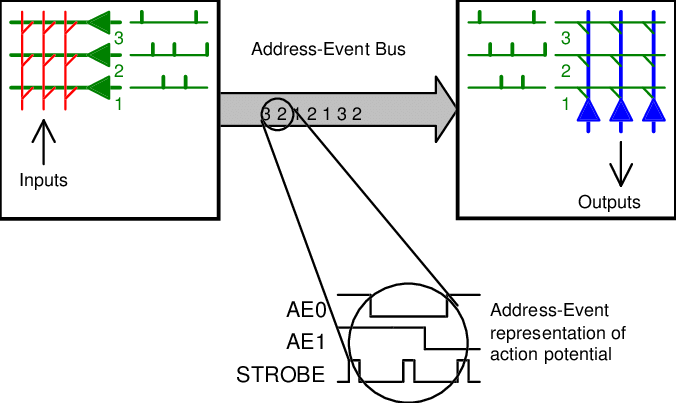
\includegraphics[width=0.5\textwidth]{Chapter2/Figs/i.png}
    \caption[The address-event representation.]{The address-event representation \cite{deiss1999pulse}. Self-timed neurons on the sending chip generate trains of action potentials. The neurons request control of the bus when they generate action potentials. They are selected to have their addresses encoded and transmitted by the multiplexing circuitry. The transmission of addresses between the sender and receiver chips occurs in a sequential manner, with each address being transferred successively. The temporal stream is processed by the receiver to produce trains of action potentials, which are subsequently transmitted to their appropriate postsynaptic targets. The relative timing of events is preserved over the address-event bus to the destination, provided that the source neurons do not generate action potentials that are excessively close in temporal proximity.}
    \label{fig:2i}
\end{figure}
    
\noindent Multiple such cores are connected via event-driven communication networks that mimic axonal signaling, typically using Address-Event Representation (AER) protocols. This allows the architecture to scale while preserving sparse, asynchronous activity similar to that found in biological systems (Figure \ref{fig:2i}). Each core processes and learns independently, while global integration arises through sparse spike-based communication.\\

\noindent One example is the Neurogrid architecture \cite{khodagholy2015neurogrid}, where analog dendritic trees are combined with digital event processors. Memristive implementations extend this idea by replacing charge-based analog memory with conductance-based synapses. The equation governing this hybrid interface may resemble:
\begin{align}
    y_j = \sigma \left( \sum_i G_{ij} \cdot V_i + b_j  \right) \label{eq:2.40}
\end{align}
\noindent Where $G_{ij}$ is the conductance of the memristive synapse, $V_i$ is the analog input voltage, $b_j$ is the digital bias term, and $\sigma$ is the thresholding or spiking function implemented digitally. \\

\noindent True biorealistic learning necessitates online, local learning, in contradistinction to traditional deep learning methods that rely on batch training and global error gradients. Memristive neuromorphic systems characteristically facilitate local learning through the implementation of pulse modulation circuits, which apply voltage updates in accordance with spike timing. \\

\noindent These systems also incorporate time-window detectors, which evaluate spike timing differences, and plasticity controllers, which adjust learning rates and homeostatic thresholds. The aforementioned engines have been demonstrated to exhibit both high levels of parallelism and low power consumption. This facilitates the capacity for real-time adaptation to dynamic inputs. For instance, a single synapse’s conductance $G$ may evolve via:
\begin{align}
    G(t + \Delta t) = G(t) + \Delta G = G(t) + f(\Delta t) \cdot V_{update} \label{eq:2.41}
\end{align}
\noindent Where $f(\Delta t)$ represents a learning window, and $V_{update}$ is the programmed voltage pulse.\\


\noindent A number of experimental systems illustrate full-stack integration of biorealistic learning in memristive networks. The Intel Loihi 2 \cite{orchard2021efficient}, equipped with emerging resistive memory, exhibits event-driven learning in a modular spiking architecture. The IMEC Dot Product Engine utilises analogue crossbars for the purpose of real-time pattern recognition \cite{zha2017imec}. NeuroSim+ is a simulation platform that validates large-scale memristive architectures with STDP and fault-tolerance \cite{chen2017neurosim+}. These systems generally comprise thousands of spiking neurons and millions of synapses, thereby facilitating the execution of complex tasks such as speech recognition, visual scene analysis, and robotic motor control. \\

\noindent Memristive architectures are regarded as optimal candidates for edge AI applications due to their compactness and low power consumption. These systems are capable of performing learning and inference directly on-device, thereby eliminating the need for cloud computation. This paradigm shift necessitates the incorporation of architectural features such as local learning with minimal supervision, non-volatile memory for state retention without power, and energy harvesting compatibility for autonomous operation. \\

\noindent From a biological standpoint, this phenomenon can be likened to the manner in which organisms acquire knowledge in an unsupervised, embodied context. This observation serves to reinforce the bio-alignment of memristive neuromorphic architectures.

\subsection[Hardware-Software Co-Design]{Hardware-Software Co-Design}

While memristive hardware presents novel capabilities for energy-efficient, biologically plausible computation, it is important to note that its full potential is only realised through careful co-design with software. In the context of biorealistic learning, and particularly in the domains of spiking neural networks (SNNs) and continuous-time recurrent systems, there is a necessity to reconsider conventional software stacks. This is so that the full potential of memristive systems, in terms of their dynamics, constraints and strengths, may be realised.\\

\noindent The majority of biorealistic models employ spiking neuron models, such as the leaky integrate-and-fire (LIF), Izhikevich, or Hodgkin-Huxley formulations. These models use time-dependent differential equations to simulate membrane dynamics:
\begin{align}
    \tau_m \frac{dV(t)}{dt} = -(V(t) - V_{rest}) + R_mI(t) \label{eq:2.42}
\end{align}

\noindent Where $V(t)$ is the membrane potential, $V_{rest}$ is the resting potential, $I(t)$ is the input current from presynaptic neurons, $\tau_m$ is the membrane time constant, and $R_m$ is the membrane resistance.\\

\noindent In order to implement such dynamics on memristive hardware, it is necessary for software frameworks to generate input spike trains, emulate conductance changes over time, encode time delays and refractory periods, and schedule event-driven computation in an efficient manner. Frameworks such as Brian2 \cite{stimberg2019brian}, NEST \cite{gewaltig2007nest}, and BindsNET \cite{hazan2018bindsnet} offer front-end abstractions for defining neuron and synapse models. From a hardware perspective, translation layers facilitate the mapping of these models to control signals, which in turn manipulate memristive devices through the utilisation of pulse sequences and voltage control. \\

\noindent Local learning rules, such as STDP or Hebbian updates, must be compiled into device-level programming protocols that adjust synaptic conductance values in response to spike timing. A significant challenge pertains to the process of quantization, wherein memristive devices exhibit constrained resolution, typically ranging from 4 to 8 bits. This limitation dictates the mapping of continuous learning gradients onto discrete conductance states during the learning update process.\\

\noindent The physical constraints of memristive arrays—such as array size, non-idealities, and fixed connectivity—call for efficient placement and routing algorithms to distribute large neural models across hardware. The key design constraints here are the fan-in/fan-out limits with physical wiring impose a restriction on the number of connections that can be established between neurons. The synaptic locality dictates that connections are most efficacious when mapped to nearby memory cells. Event congestion, characterised by the influx of spikes, can lead to the saturation of routers if not load-balanced.\\

\noindent In order to optimise for these constraints, mapping tools employ graph partitioning and spatial locality heuristics. This ensures that neurons which interact frequently are co-located, synapses with high activity are placed on reliable memory cells, and event routing is sparse and non-overlapping. Memristive devices are inherently stochastic and are subject to issues such as cycle-to-cycle variability, device-to-device variation, drift and age-related degradation. The utilisation of software-based compensation algorithms has been identified as a means of mitigating these effects. \\

\noindent Examples of such methods include the write-verify loop is a programming technique that involves the iterative modification of conductance parameters until a predetermined target is attained. Adaptive learning rates are a process which adjust update magnitude dynamically based on noise. Redundancy encoding involves the distribution of synaptic weights across multiple devices, a strategy that is employed to enhance robustness. Moreover, homeostatic plasticity—a biologically inspired process where neuron activity is stabilized—can be implemented as a system-level feedback mechanism:
\begin{align}
    \theta_i(t + 1) = \theta_i(t) + \eta(r_i - r_{target}) \label{eq:2.43}
\end{align}

\noindent Where $\theta_i$ is the threshold of neuron $i$, $r_i$ is the recent firing rate, $r_{target}$ is the target firing rate, $\eta$ is the adjustment rate. This allows software to dynamically regulate hardware behavior to match desired spiking statistics.\\

\noindent Given the cost of prototyping new memristive chips, emulation platforms assume a pivotal role. These systems simulate the behaviour of memristive networks using digital hardware, such as field-programmable gate arrays (FPGAs), or software, for example Python/C++ models, while preserving the timing and constraints of real devices. \\

\noindent For instance, NeuroSim and MNSIM offer device-aware simulation of crossbar-based spiking neural networks (SNNs), CARLsim supports GPU-accelerated emulation of spiking networks with STDP, and XNOR-Nets simulate low-precision inference to match memristive behaviour. These pipelines facilitate the testing of novel learning rules, the evaluation of scalability, and the validation of functional accuracy prior to the commitment of resources to silicon implementation.\\

\noindent To bridge the gap between algorithm design and hardware execution, domain-specific languages and toolchains have emerged such asNengo, A high-level API for building SNNs with hardware backends. PyNN, A Python interface supporting multiple simulators and hardware targets. Loihi's NxSDK: A low-level toolchain for configuring on-chip learning and routing. \\

\noindent Memristive neuromorphic systems are starting to integrate with these ecosystems, allowing a complete workflow in the following steps Model specification, Learning rule assignment, Hardware mapping, Runtime adaptation. The future of biorealistic learning on memristive networks depends on such co-designed environments that abstract away hardware complexity while maintaining biological plausibility and computational efficiency.

\subsection[Experimental Validations Strategy]{Experimental Validations Strategy}

Experimental validation is crucial to assessing the practical effectiveness of biorealistic learning algorithms implemented on memristive networks. This section explores the empirical studies and benchmark tasks used to evaluate the performance of these systems, including comparisons with traditional digital hardware platforms and biological neural networks. Furthermore, the challenges and potential solutions for validating neuromorphic systems on memristive hardware are discussed. \\

\noindent In order to assess the robustness and efficiency of memristive neural networks (MNNs), it is customary to utilise a number of benchmark tasks. The tasks have been meticulously designed to evaluate various aspects of learning, generalisation, and computational efficiency. The primary categories of benchmarks comprise pattern recognition and classification tasks, the purpose of which is to evaluate the capability of a network to identify patterns in data. \\

\noindent The MNIST dataset is a commonly cited example of a set of handwritten digits. It is frequently employed to evaluate the fundamental classification capabilities of neuromorphic systems. CIFAR-10/100 is employed for the classification of images in tasks intended to evaluate the performance of networks when dealing with more complex visual data. Memristive networks are utilised for speech recognition tasks, encompassing the identification of spoken words or phonemes, thus providing a test case for temporal pattern recognition.\\

\noindent The evaluation of the ability of memristive networks to store and recall information is facilitated by memory and learning tasks. Examples include sequence learning, which tests the system's ability to learn temporal sequences (e.g. speech or music recognition tasks), and working memory, which evaluates the system's ability to hold and manipulate information over time (a critical aspect of biorealistic learning). \\

\noindent Furthermore, the tasks employed in reinforcement learning evaluate the capacity of a network to optimise actions in accordance with environmental feedback, thereby simulating the adaptive characteristics of biological learning processes. For instance, Atari games have been utilised to evaluate the efficacy of memristive networks in acquiring sophisticated decision-making methodologies from pixel-based inputs. \\

\noindent Each of these benchmarks serves the purpose of evaluating various performance metrics, including accuracy, which is defined as the percentage of accurate predictions or classifications made by the network; speed of learning, which is defined as the network's capacity to rapidly adapt to novel activities or scenarios; and efficiency of energy, which is measured by the ratio of energy usage per job. In order to assess energy consumption, memristive systems are often compared with traditional digital hardware platforms.\\

\noindent Empirical studies involving memristive systems typically explore how memristive devices can be utilized to implement spiking neural networks (SNNs), leveraging both the computational power of memristive crossbar arrays and the temporal dynamics of biological neural models. In studies evaluating pattern recognition tasks (such as MNIST classification), memristive networks have demonstrated competitive results when compared to conventional deep learning algorithms. \\

\noindent One example comes from the use of crossbar arrays with spike-timing-dependent plasticity (STDP) learning rules. A study using a 4-layer SNN on memristive hardware showed up to 97\% accuracy.  This result was achieved with an energy consumption reduction of up to 30\% compared to a traditional GPU-based deep learning model for similar accuracy. \\

\noindent In memory tasks, such as sequence learning and working memory, memristive systems excel in their ability to emulate biological learning processes. A study utilizing a memristive recurrent neural network (RNN) for sequence prediction demonstrated that:
\begin{align}
    E = \frac{1}{N} \sum_{i=1}^{N} \left| y_i - \hat{y}_i  \right| \label{eq:2.44}
\end{align}

\noindent Where $E$ is the error, $y_i$ is the true output, and $\hat{y}_i$ is the predicted output.  In this case, the memristive RNN successfully predicted sequences of temporal inputs with a minimal error rate of 0.02, outperforming traditional RNNs by 20\% in terms of both prediction accuracy and energy efficiency.\\

\noindent Memristive networks also show promise in reinforcement learning tasks. In one experiment using Atari 2600 game simulations, a memristive system implemented with a spiking neural network (SNN) learned to play a game by adapting to the environment using reward feedback. The memristive SNN employed a biologically inspired reward-modulated plasticity rule:
\begin{align}
    \Delta w_{ij} = \eta \cdot \left( r_i - \alpha \cdot w_{ij} \right) \label{eq:2.45}
\end{align}

\noindent Where $\eta$ is the learning rate, $r_i$ is the reward, $\alpha$ is the decay factor, and $w_{ij}$ represents the weight between neurons $i$ and $j$. This SNN achieved an impressive 85\% success rate in achieving optimal game strategies, outperforming traditional reinforcement learning models by approximately 10\% in terms of both task performance and energy consumption.\\

\noindent One of the main advantages of memristive systems is their energy efficiency. Compared to traditional von Neumann architectures, memristive devices excel at massively parallel computation with low energy cost. When implementing algorithms such as STDP, memristive networks require significantly fewer energy resources. For example, a memristive chip consuming 1 watt can perform tasks that would require 100 watts on a conventional CPU or GPU. \\

\noindent Moreover, the non-volatility of memristive devices allows for permanent synaptic weight storage, which is particularly useful for neuromorphic systems that operate continuously and in real-time. This feature reduces the need for frequent memory refresh operations, making memristive systems inherently more power-efficient.\\

\noindent Despite these advantages, there are inherent challenges in scaling memristive networks. Memristive devices suffer from device-to-device variations, where the conductance change may differ between identical devices due to manufacturing differences. These discrepancies must be handled via calibration techniques or redundancy. \\

\noindent As the number of memristive devices on a chip increases, the risk of crosstalk (interference between adjacent devices) also increases. To mitigate this, advanced routing and encoding strategies must be employed to isolate signal paths and minimize errors. Memristive devices generally offer lower precision compared to traditional digital circuits. To handle this, techniques like quantization, error correction, and approximate computing can be utilized to maintain system performance within acceptable bounds.\\

\noindent As research progresses, experimental validations are likely to evolve to explore more complex real-world tasks. In the field of brain emulation, significant progress has been made in recent years, with research focusing on the development of large-scale networks that emulate the complex functions of the human brain. These networks utilise memristive chips, which have emerged as a key component in the modelling of higher-order cognitive processes, such as reasoning, decision-making, and emotional responses. The future direction of this research is expected to involve the creation of more sophisticated networks that can model these cognitive functions more accurately and effectively, paving the way for new applications in fields such as artificial intelligence and neuroscience. \\

\noindent The integration of neuroprosthetics with memristive systems into wearable neural interfaces has the potential to augment or restore sensory or motor functions in humans. The integration of synthetic biology in future studies may explore the convergence of memristive networks and synthetic biology, where biological neurons and memristive devices coexist in hybrid systems for the purpose of enhancing learning capabilities. The long-term potential of memristive neuromorphic systems lies in their ability to mirror biological computation, offering vast improvements in energy efficiency, processing power, and scalability.

\section[Summary]{Summary}

\noindent Memristive networks are a state-of-the-art approach to creating systems with the capacity for biorealistic learning and adaptive behaviour. Memristive devices have been shown to possess a unique capacity for modelling synaptic plasticity, thereby facilitating the development of mimetic computational processes that emulate those observed in biological systems. The potential applications of these systems are extensive, ranging from robotics and AI to neuroprosthetics and brain-computer interfaces.\\

\noindent As research continues to address the challenges of device performance, scalability, learning algorithms, and integration with biological systems, the full potential of memristive networks is becoming more apparent. Nevertheless, it is imperative that these advancements are accompanied by a meticulous examination of the ethical and societal ramifications of these technologies.\\

\noindent In the coming years, it is anticipated that a paradigm shift will occur in the manner by which machines learn and interact with the world. This revolution will be spearheaded by memristive networks. The development of biorealistic learning on memristive networks has the potential to create more intelligent, adaptive, and energy-efficient systems, with the capacity to transform fields as diverse as robotics, AI, neuroscience, and medicine.
%!TEX root = ../thesis.tex
%*******************************************************************************
%****************************** Third Chapter **********************************
%*******************************************************************************
\chapter{Fabrication and Characterisation Methodologies}


\section[Fabrication Procedure]{Fabrication Procedure}

It is imperative that the capability of the devices to exhibit distinct and stable state-dependent conductance changes is demonstrated prior to the design of novel neuromorphic systems. These conductance changes are modelled in neuronal spiking systems. \\

\noindent The present chapter thus provides a detailed account of the experimental methodology employed in this study, alongside a comprehensive presentation of the results obtained from the experiments. The aforementioned devices have been demonstrated to exhibit a variety of non-volatile switching properties. The measurements are focused on the electrical characteristics and switching mechanism of the samples. \\

\noindent The devices investigated in this thesis were developed by the Electronic Materials and Devices group in the department. Despite the fact that the fabrication process was described in detail here for completeness, some tasks described here were not personally carried out, therefore certain credits go to the rest of the research group.

\subsection[Device Properties]{Device Properties}

\noindent The device investigated in this thesis has a metal-insulator-metal (MIM) structure and is manufactured on a silicon wafer. A thick silicon dioxide layer is thermally accumulated onto the wafer preparatory to the bottom electrode to prevent interactions between the bottom metal contact and the wafer. After that, the bottom electrode and thin film oxide are deposited unpatterned throughout the whole sample. Finally, during the deposition process, the top electrical contacts are patterned into squares with sides varying from $200\mu m$ to $800\mu m$ in Figure \ref{fig:3a}. Photolithography is not employed for patterning since a contact mask is used. \\

\begin{figure}[htbp!] 
    \centering    
    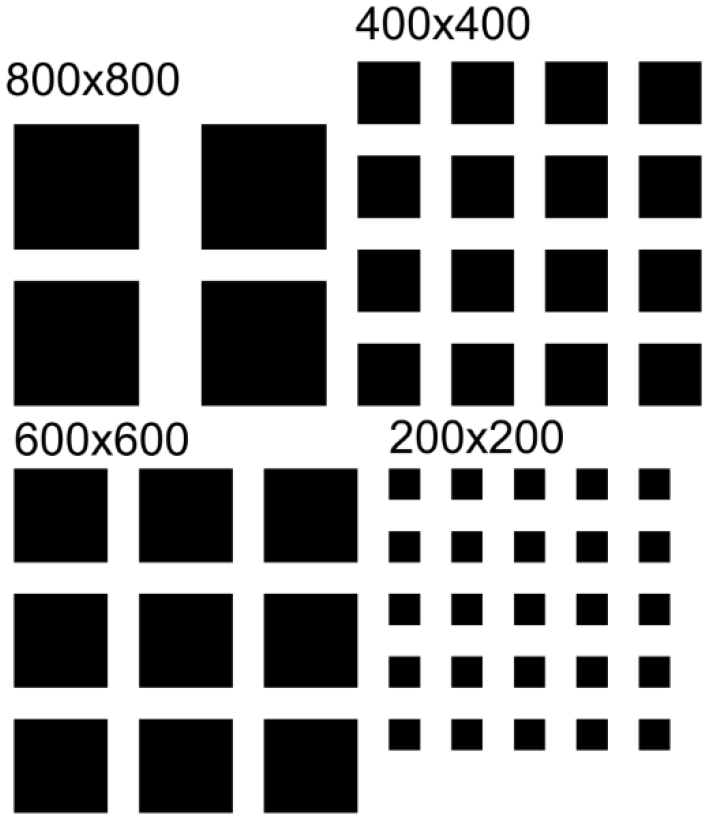
\includegraphics[width=0.8\textwidth]{Chapter3/Figs/a.png}
    \caption[Device Structure]{Photolithographic mask (left) and dimensions of the top electrical contact (right).}
    \label{fig:3a}
\end{figure}

\noindent To increase adhesion, a second titanium buffer layer is placed between the top metal contact and the oxide. This adhesive layer is less than ideal since it can cause additional imperfections to migrate within the oxide. Despite this worry, research using electron energy loss spectroscopy (EELS) and transmission electron microscopy (TEM) have shown no evidence of titanium interface migration in the devices \cite{mehonic2017intrinsic}. \\

\noindent The utilisation of gold as a primary electrical contact may result in the migration of gold atoms into the oxide layer and their subsequent diffusion through the film. For instance, a study conducted into the diffusion of gold through amorphous SiOx observed the migration of gold into the oxide when the gold was held at a temperature of $390^{\circ} C$ for a period of four hours \cite{madams1974migration}. \\

\noindent Furthermore, it was established that when the gold was exposed to a temperature of $500^{\circ} C$ for a duration of two hours, it was observed to be distributed uniformly throughout the oxide layer, which had a thickness of approximately 500 nm. Nonetheless, no migration was observed at temperatures below $370^{\circ} C$. Although the diffusion of gold through silicon oxide films at elevated temperatures has been observed, this phenomenon is frequently disregarded or presumed to be non-occurring in devices utilised as resistance switching memories. \\

\noindent In the domain of electrochemical metallisation, where metallic filaments are formed between two electrodes, gold is recognised as an inert electrode \cite{kozicki2016electrochemical}. This principle is also widely accepted in the context of valence change memories \cite{ge2014electrode}. In one particular instance of a device composed of gold and silver electrodes that were sandwiched between an $As_2S_3$ film, only the migration of silver was observed. \\

\noindent This migration resulted in the formation of a conductive bridge between the contacts \cite{hirose1976polarity}. The stability of the gold contacts within this application is assumed to be due to the fact that device operation is restricted to room temperature experiments. Alternatively, the presence and migration of a comparatively more active/mobile electrode, such as silver, may have a more significant effect on device properties.\\

\noindent It has been claimed that asymmetry in the device's construction, as well as an active and inert electrode, are necessary to identify stable switching. The molybdenum contact can be crucial as an oxygen reservoir, rapidly exchanging oxygen between the electrode and silicon oxide layer, which is similar to an active electrode, according to a recent experiment \cite{cox2021nanoscale}. The materials used for the top and bottom electrodes are different and weren't explicitly chosen for this project; rather, other group members had already picked them to create high-performance resistance switching memory. \\

\noindent The device layers remain mostly unchanged throughout the investigation. The top electrical contact is made of a different material in the experiment than the bottom electrical contact, which is made of a thin film of molybdenum. The oxide layer is made of an amorphous silicon oxide thin film. The selection of gold as the top electrical contact may cause gold atoms to diffuse through the film and migrate into the oxide. \\

\noindent Although gold has been seen to diffuse through silicon oxide layers at high temperatures, resistance switching memory frequently overlook this phenomenon or presume it does not happen. A profilometer is used to assess the thickness of the layers. To guarantee excellent conductivity throughout the device, the bottom electrode is 300 nm thick. The oxide slim film is 35nm in depth. The thickness of the top electrical contact varies depending on the substance; gold has a thickness of 110 nm, while ITO has a thickness of 50 nm.

\subsection[Manufacturing Steps]{Manufacturing Steps}

\noindent RF sputtering, a physical vapour deposition process, was used to deposit all of the device layers. Deposition is carried out at low pressure in a typical inert gas environment by blasting the intended material with a plasma, which causes the expulsion of atoms from the target. Depending on the gas pressure inside the chamber, the expelled atoms either follow a direct ballistic path or take a random walk until they land on the sample. A greater gas pressure will result in more collisions and an increased random walk, whereas a lower gas pressure produces a more direct ballistic trajectory. \\

\begin{figure}[htbp!] 
    \centering    
    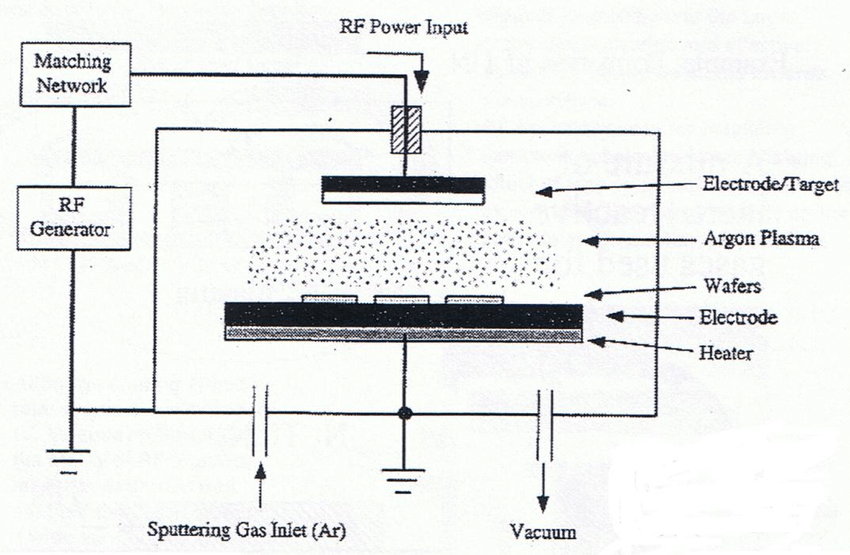
\includegraphics[width=0.6\textwidth]{Chapter3/Figs/b.png}
    \caption[Radio Frequency Magnetron Sputtering]{Depiction of the fundamental configuration for the deposition of thin films by means of sputtering \cite{jeong2008origin}. A substantial radio frequency electric field is required to ionise argon gas, thereby producing a plasma. The process of deposition is initiated by high-energy collisions between the ionised argon and the target material. The collisions result in target atoms being ejected from the source with high kinetic energy. These atoms traverse the chamber and deposit onto the sample over time, thereby forming an amorphous thin film.}
    \label{fig:3b}
\end{figure}

\noindent A simplified version of the sputtering system is illustrated in Figure \ref{fig:3b}. The configuration under consideration comprises the sample, which is connected to the anode of the RF power source, the target material, which is situated in front of the cathode, and the sputtering gas, which is injected into the chamber. The plasma is composed of argon ions, which possess a positive charge. These ions are attracted to the cathode, which is negatively charged and is therefore known as the target. The process of high-energy collisions between argon ions and the target surface is a prerequisite for the ejection of target atoms.\\

\noindent  The substance being deposited, known as the target material, is initially solid. By applying a strong electric field to the sputtering gas (argon), the plasma is created. Either a DC or an AC field is possible. However, an AC field that oscillates at an RF frequency of 13.56MHz is necessary for dielectric targets like $SiO_2$. Sputtering often results in amorphous films with sub-stoichiometric oxides. The devices' SiOx oxide has a stoichiometry of 1.9, while the film's roughness appears to be determined by the RMS roughness of the underlying molybdenum layer, which ranges from 0.9 to 1.5 nm \cite{kenyon2019interplay}. \\


\begin{figure}[htbp!] 
    \centering    
    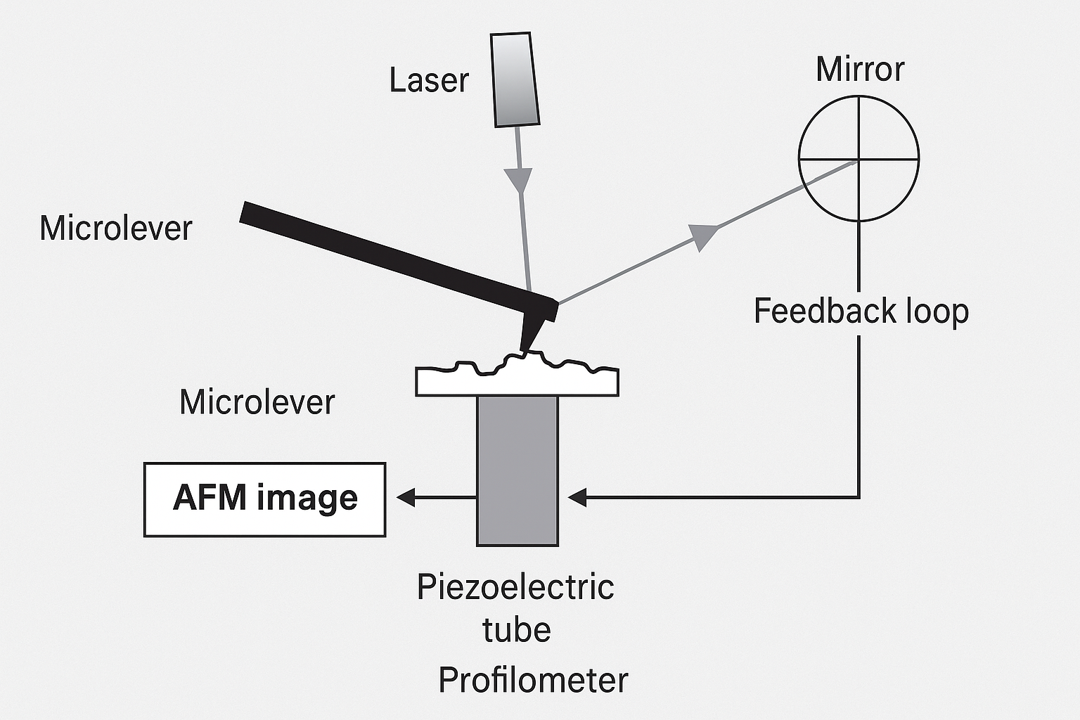
\includegraphics[width=0.6\textwidth]{Chapter3/Figs/c.png}
    \caption[Contact profilometer for thin film thickness measurements.]{Schematic of a profilometer \cite{mabilleau2008vitro}. The probe is utilised to scan the surface of the sample, with the height of the probe being adjusted accordingly in order to ensure that a constant force is maintained. It is imperative to note that a feedback loop is utilised in order to ensure the maintenance of this force during the process of reporting the tip height. The measurement of thin film thicknesses following deposition is achieved through the fabrication of a staircase-like structure.}
    \label{fig:3c}
\end{figure}

\noindent In the course of each SiOx sputtering run, a pair of Si substrate specimens are inserted into the chamber in conjunction with the sample for the purpose of thickness measurement. In the first instance, a specific region of the Si substrate is masked using a patterned photoresist. Following the process of SiOx deposition, the mask material is removed using a solvent, thereby creating a step on the SiOx/Si interface. \\

\noindent The measurement of this step is then undertaken with the aid of a Dektak XT profilometer, which is capable of resolving a step height of a few nanometres. The second piece of Si substrate, which has been covered with SiOx, is then measured using ellipsometry. This is a process that is used to verify the thickness of the deposited layer.\\

\noindent After being sputtered, film thickness is measured via a contact profilometer with a 0.5nm precision. During this procedure, a diamond tip is used to make contact with the sample and scan across the surface. Utilising a feedback loop, the tip's height is adjusted to maintain a consistent force against the sample's surface as it scans, giving the measurement of the sample height. The sample's surface height changes in direct proportion to the change in tip height. Layer thicknesses of a device stack are measured in relation to one another using a staircase-like pattern that is created during production. 

\subsection[Experimental Setup]{Experimental Setup}

The amount of current passing through the device is the significant observable. This includes details on the oxide layer's bulk conductivity as well as the interface barrier heights. The difficulty, however, is in minimising any deviations or nonlinearities brought on by the measuring apparatus itself, with probe contact resistance serving as one such example. It is necessary to choose how to make contact with the device electrodes before conducting current measurements. There are essentially two methods: either the circuit is wire bonded inside a chip carrier, or the contacts are directly probed with tiny metallic probes using micromanipulators. \\

\noindent The direct probing method utilising tungsten probes has been adopted instead due to the devices' design and susceptibility to break from the wire bonding procedure. The tip of the probe must be brought down carefully to prevent damage. When placing the probe into contact, a low voltage is often supplied as a test signal. \\

\noindent To determine if the probe has made contact, the current is watched for a spike in the device current. Initially, because there is no measurable electrical current while the probe is not in touch with the device, the current oscillates around positive and negative currents at 0 amps. Once the probe makes contact with the device, the voltage that has been applied across it now causes a detectable current that matches the polarity of the applied voltage. \\

\noindent In contrast to the probe method, which can be vulnerable to sample damage brought on by the experimentalist, the wire-bonded approach has the advantage which the position of the electrical connection does not change between experiments, thermal expansion while temperature measurements will not significantly affect the contact, and there is less risk of deteriorating the device throughout characterisation. \\

\noindent However, there is a chance that the component will be broken during the bonding procedure with wires. An ultrasonic pulse is utilised to melt a gold or aluminium wire to the device contact while applying pressure to help fuse the two metals together. It has been regularly observed that this pressure can cause internal layers to compress, leading to electric shorts between the two metal contacts and ultimately damaging the device. \\ 

\begin{figure}[htbp!] 
    \centering    
    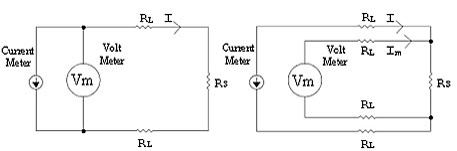
\includegraphics[width=0.8\textwidth]{Chapter3/Figs/d.png}
    \caption[Two wire or Four wire (Kelvin) testing.]{Two wire or Four wire (Kelvin) testing. A schematic of the 2-wire measurement setup is provided herewith. The voltage (VSource) is applied to the sample using two probes. It is important to note that each probe introduces a series resistance (Rprobe) with the sample's resistance (Rsample). The device current (Imeas) is measured by an ammeter in series. Conversely, a constant current (Isource) is supplied through the sample by two probes. The voltage induced across the device (Vmeas) by the current is measured with a voltmeter in parallel with the sample.}
    \label{fig:3d}
\end{figure}

\noindent After deciding on a contact technique, the next choice is how currents will be monitored. Both a 2-wire measurement and a 4-wire measurement are frequently available as options. The sample's conductivity serves as the basis for the decision. The easiest way to measure electrical resistance is to apply a set voltage and track the total current passing through the object. Only two electrical connections are formed, thus the term "2-wire measurement" for this procedure. Ohm's Law is used to determine the device resistance by connecting a voltage source, an ammeter, and the device in series. \\

\noindent Due to the assumption that the electrical resistance is only determined by the test device, which is not true in reality where there are several sources of electrical resistance connected in series with the device, this measurement is often not correct. These include the wires connecting the test object and the voltage source, the internal resistance of the voltage source or the ammeter, and, especially, the contact resistance that develops at the point where the electrical probes and the test object meet. \\

\noindent One of the most crucial parameters to take into account when describing thin films is contact resistance, which may be reduced by placing metal contacts on the sample during manufacturing. Fortunately, the device resistance usually outweighs the electrical resistance, making this method valid in the majority of instances. However, when resistance is small, the parasitic resistances of the measuring circuit become notable and must be eliminated by using a 4-wire resistance measurement. \\

\noindent Ohm's law is still used in this configuration to calculate resistance. Instead of sourcing a voltage and monitoring a current, the device is subjected to a steady current that induces a voltage across it. Through two extra probes connected in parallel to the device, a voltmeter measures the potential decrease. It is crucial to recognise that the same contact resistance and wire resistances that plagued the 2-wire method continue to exist for all four connections. However, in this case, the high impedance of the voltmeter causes a substantially lesser current to pass through the measuring contacts. \\

\noindent The voltage recorded by the voltmeter is thought to more precisely represent the voltage drop across the device since the voltage dip across the parasitic resistance is insignificant. This occurs because the voltage produced across the contact resistance is lowered as a result of the reduced current flowing through the probes, which detect the voltage across the device. By lowering these voltages, which are induced across each probe's contact resistances and contribute mistakes into the voltage measurements, it is possible to measure the voltage across the device with more accuracy. \\

\noindent Thus, the device resistance determines whether to use a 2-wire or 4-wire resistance measurement. The devices examined in this work have high resistance, ranging from kilo-ohms to mega-ohms. The parasitic resistances of the measuring circuit, like the contact resistances, are insignificant at this level. The issue of measuring device currents must now be solved once the device has been attached. Again, there are a variety of techniques that might be applied; the one selected will often depend on the size of the current being measured. \\

\noindent The most elementary method of measuring current is to use a digital multimeter (DMM) ammeter. The device functions in accordance with Ohm's law, utilising the principle of electrical resistance to measure the voltage drop across a fixed resistor, commonly referred to as the shunt resistor. Whilst the validity of this approach is indisputable for currents within the milliamp range and above, issues arise for lower current levels due to the noise induced by the shunt resistor.  In order to measure smaller currents, larger shunt resistors are required. This, however, gives rise to two problems. \\

\noindent Firstly, it is important to note that larger resistors are known to introduce greater thermal noise, which has the capacity to disturb the voltage being measured. Secondly, an increase in resistance results in an increase in the voltage drop across the ammeter. The voltage drop, termed the 'voltage burden', becomes problematic when its magnitude is no longer negligible in comparison to the voltage applied to the device under test. The combination of voltage burden and the thermal noise of the shunt resistor invariably imposes a lower limit on current measurements when a DMM is employed. \\

\noindent The average current range for the devices is 100nA to 1mA, therefore a picoammeter is required to detect considerably lower currents on the order of picoamps to nanoamps. Picoammeters minimise current readings by a number of methods that differ across manufacturers. The majority of them employ a transimpedance amplifier to magnify the signal while an op-amp converts the input current to a voltage. Once again, how this is implemented differs from manufacture to manufacture and is frequently protected intellectual property that is not revealed. \\

\begin{figure}[htbp!] 
    \centering    
    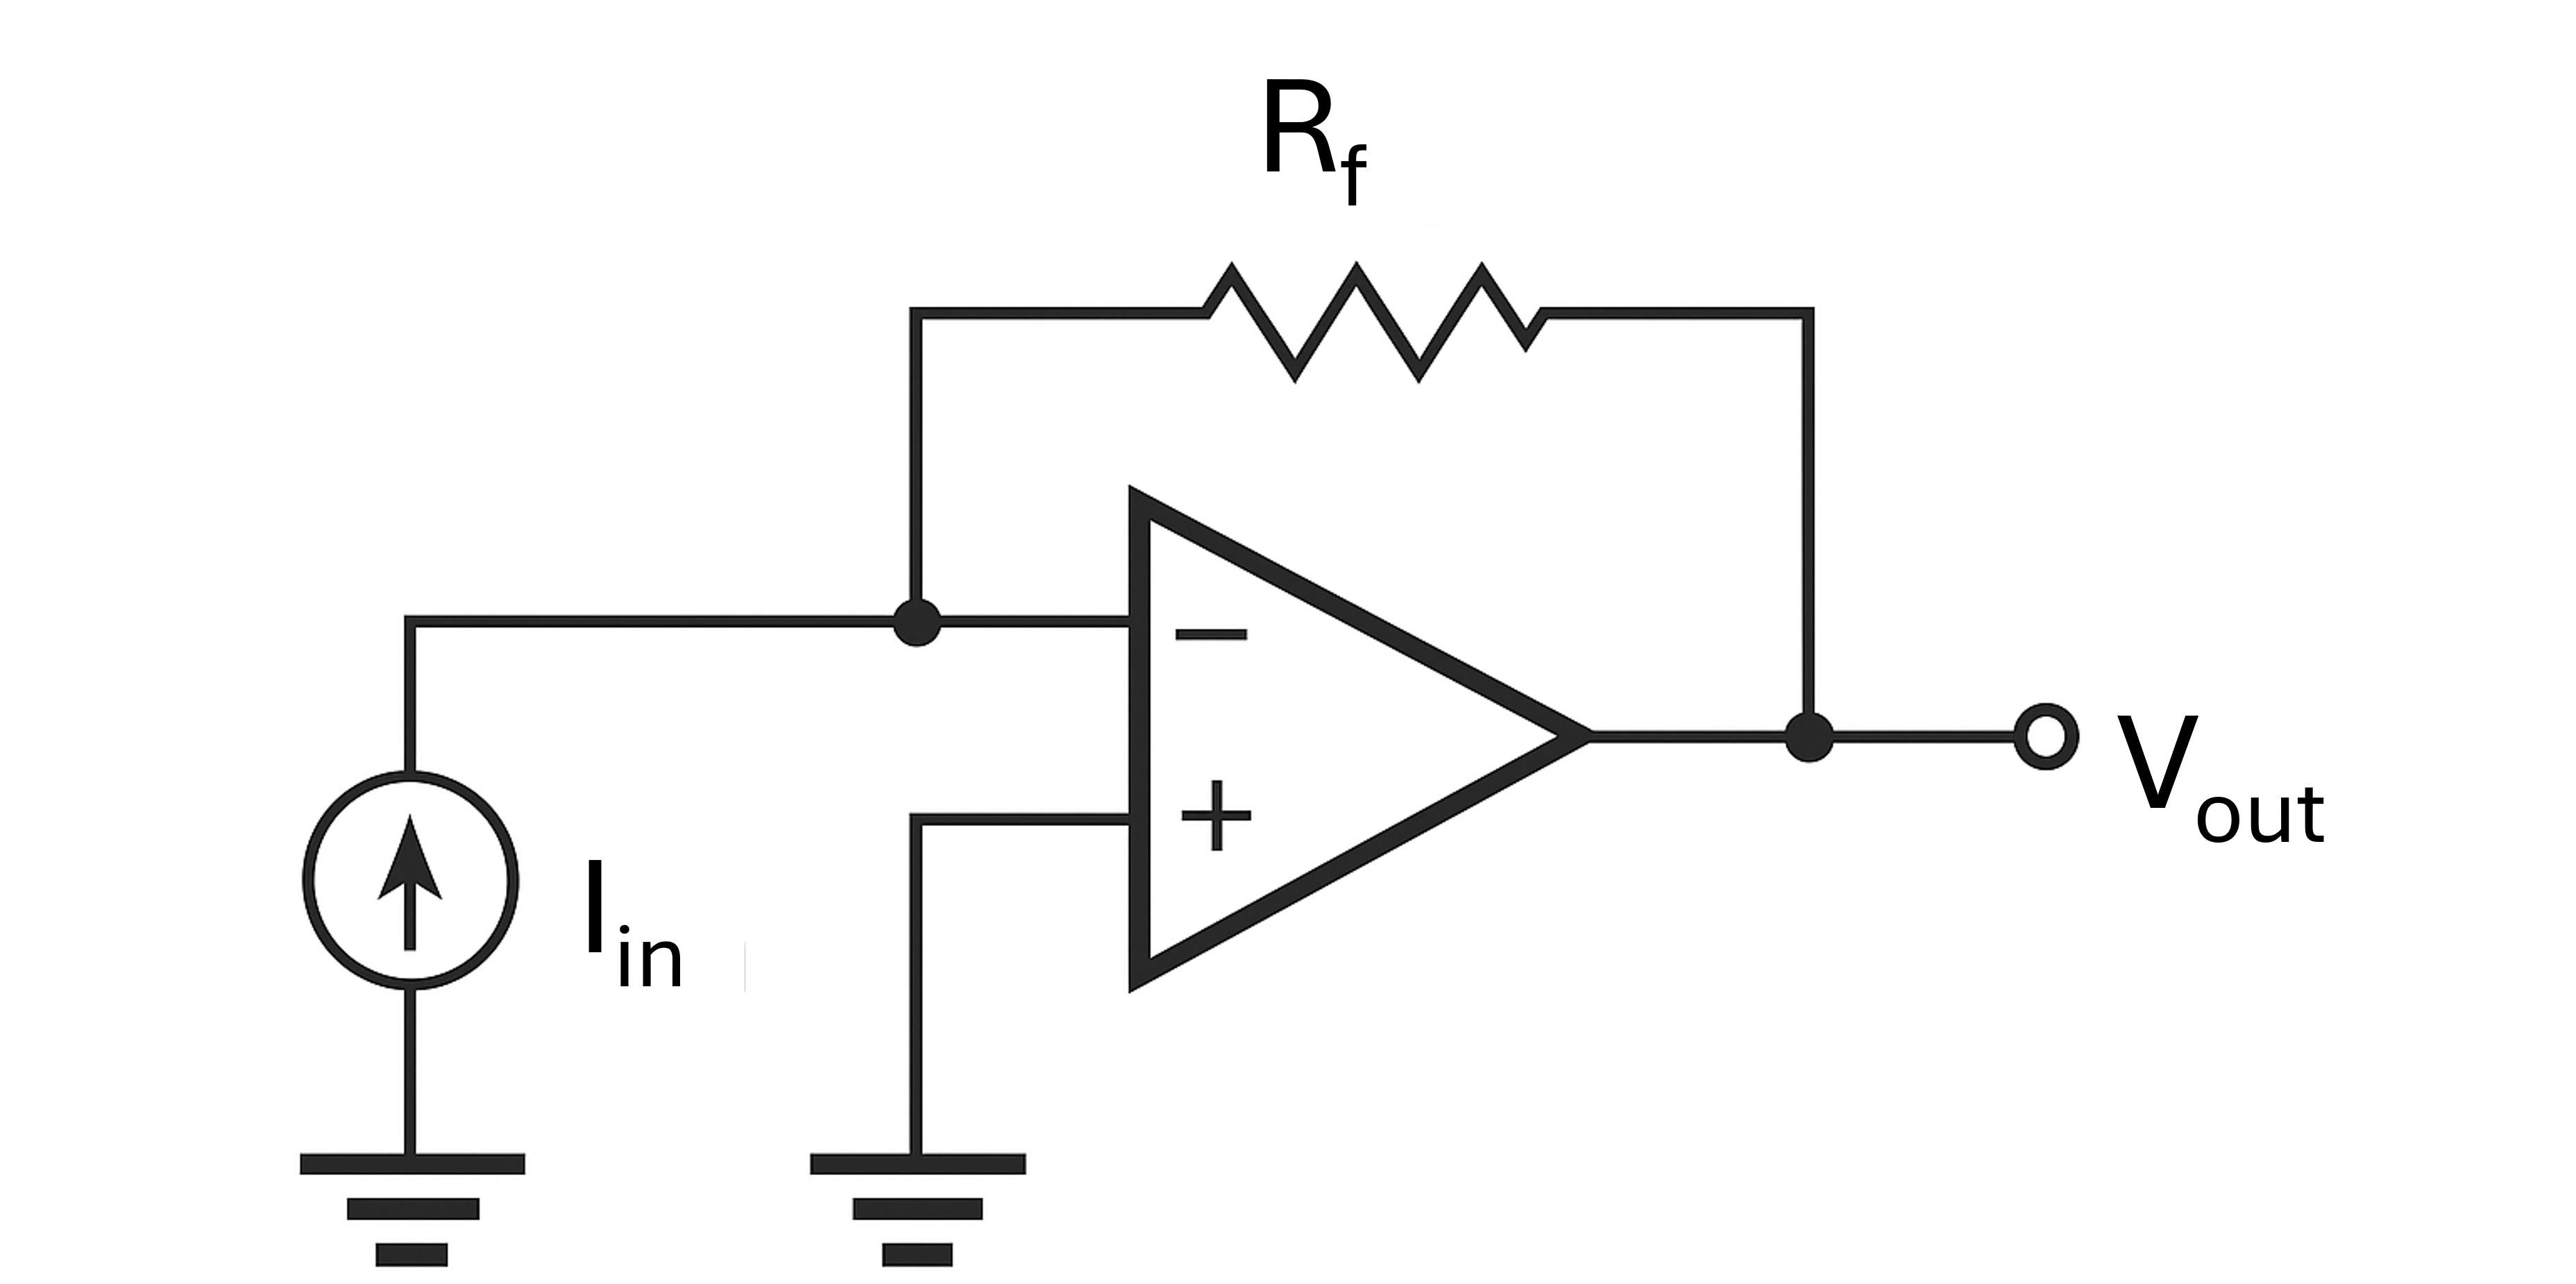
\includegraphics[width=0.5\textwidth]{Chapter3/Figs/e.png}
    \caption[Transimpedance amplifier circuit.]{Transimpedance amplifier circuit. The input current ($I_{in}$) is amplified and converted into an output voltage ($V_{out}$) via the operational amplifier. The gain is defined by the feedback resistor (RF). The voltage/current ($V_{out}/I_{in}$) is equivalent to negative resistance ($-R_f = V_{out} / I_{in}$).}
    \label{fig:3e}
\end{figure}

\noindent Nevertheless, the general operation can be comprehended with the aid of the circuit in Figure 8. The circuit under consideration is a transimpedance amplifier, the function of which is to convert the input current ($I_(in)$) to an output voltage ($V_(out)$). The operational amplifier is known to adjust its output voltage in order to reduce the voltage difference between its two input pins, designated as '-' and '+'. In this circuit, the non-inverting input pin (+) is grounded. This action causes the operational amplifier (op-amp) to adjust its output voltage, thereby ensuring that the voltage at the inverting input pin (-) is also zero volts. \\

\noindent The application of an input current to the circuit results in a transient voltage offset at the input pin. The op-amp rapidly adjusts the output voltage, thereby inducing a current of equal and opposite magnitude through the feedback resistor. This, in turn, results in the cancellation of the input current. The voltage at the inverting pin (-) is rapidly returned to zero by the feedback from the operational amplifier, thereby creating a virtual ground. \\

\noindent The generation of this inverse current ($I_{inv}$) is accompanied by the definition of the voltage at the output of the operational amplifier in accordance with Ohm's law: It can thus be demonstrated that the voltage is $V_{out} = -R_f \cdot I_{inv}$, resulting in a voltage that follows the input current. The amplification of this voltage is defined by the feedback resistor, $R_f$. The virtual ground is a key advantage of this technique. The consequence of this is a significant reduction in the voltage burden, since the shunt resistor that was previously connected in series with the device under test has now been removed. This facilitates the measurement of smaller currents, which would not have been possible using a DMM due to the significant voltage burden caused by the sensing resistor. \\

\noindent It is evident that, in view of the aforementioned factors, the utilisation of a picoammeter constitutes the optimal instrument for the execution of current-time measurements or current-voltage sweeps on our devices The equipment used in this instance is the Keithley 6430 sourcemeter, which combines a picoammeter and a low noise voltage source into a single device. \\

\begin{figure}[htbp!] 
    \centering    
    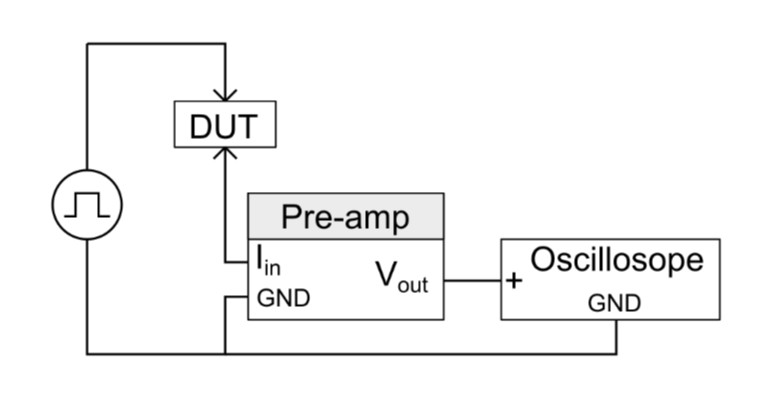
\includegraphics[width=0.8\textwidth]{Chapter3/Figs/f.png}
    \caption[Experimental setup of spike train measurements.]{Experimental setup of spike train measurements. Spike trains are generated using an arbitrary signal generator. The device current is amplified and converted into an output voltage via the preamplifier, which is connected in series with the device. The output of the current preamplifier is then captured by an oscilloscope.}
    \label{fig:3f}
\end{figure}

\noindent In some cases, the device requires the application of voltage transients that are more complex than step potentials, such as pulses or custom spike trains. In these cases, the Keithley's sampling frequency is insufficient to generate such signals. An arbitrary signal generator is used in its place to create voltage transients, and a current preamplifier is connected in series with the device to amplify device currents. In particular, the oscilloscope (Rigol DS4024) and current preamplifier (SR570) are used.

\section[Electrical Characterisation]{Electrical Characterisation}

\noindent Resistive switching is defined as a reversible phenomenon that occurs in two-terminal elements. In a non-volatile manner, these devices undergo a change in resistance when subjected to electrical stimuli. In the case of ReRAM devices, it is a local redox process that dictates the resistive switching mechanism. The reversibility of the process is achieved by the repeated application of suitable stimuli. This mechanism governs the resistance values between two or more levels. \\

\noindent The predominant phenomenon observed in these devices is resistive switching. For the sake of convenience, the switching states of the memristor can be defined. The assignment of high resistance to the "OFF" state and low resistance to the "ON" state is intuitive, with a contrast in resistance by a few orders of magnitude. The transition from the high resistance state (HRS) to the low resistance state (LRS) is defined as "Set", while the reverse is defined as "Reset". In many cases, an initial electroforming process is required to transform the device from a pristine state to a switchable state. It is generally accepted that the pristine device exhibits a higher degree of resistance than the HRS.\\

\noindent The majority of metal oxide devices exhibit either unipolar or bipolar switching. In contrast, both unipolar and bipolar switching can be observed in our silicon oxides. The preliminary characterisation of these devices encompassed the fundamental I-V characteristics. The experimental procedure involved the execution of the tests utilising the dual sweep functionality of the Keithley 4200-SCS, employing two tip probes with a diameter of 10 $\mu m$. Testing was performed on both sets of samples across all electrode pad sizes.

\subsection[Unipolar Switching Mode]{Unipolar Switching Mode}

\noindent Initial electroforming is a prerequisite for switching in these devices. It is generally accepted that fresh samples are in a very HRS, which necessitates the application of a significant electrical stimulus to enable the cell to transition into LRS for the first time. Subsequent to this preliminary phase of formation conditioning, the apparatus may be reversibly switched between two bi-stable states. \\

\begin{figure}[htbp!] 
    \centering    
    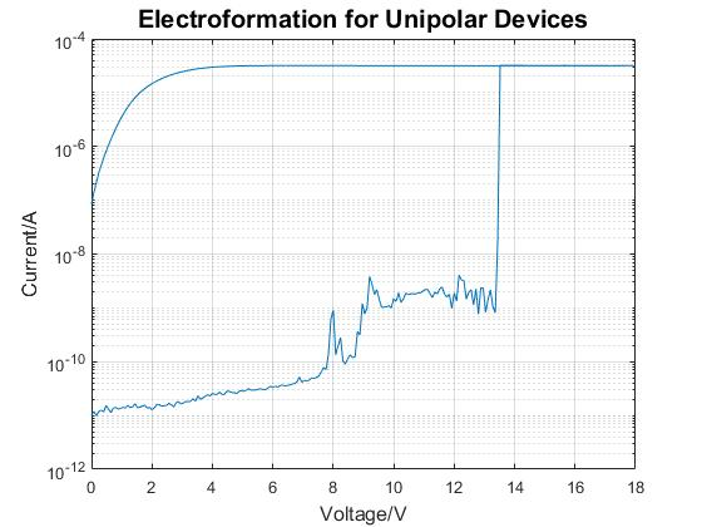
\includegraphics[width=0.6\textwidth]{Chapter3/Figs/g.png}
    \caption[Initial Electroformation step for unipolar switching.]{Initial Electroformation step for unipolar switching via a double sweep curve.}
    \label{fig:3g}
\end{figure}

\noindent The electroforming operation is widely regarded as a form of electrical breakdown, which is critically dependent on current-limiting mechanisms to ensure the subsequent switching functionality of the cell. Current limitations may be addressed by leveraging the existing compliance functionality of the Keithley-SCS. In certain instances, the analyser may exhibit a slower response rate than the formation process itself, resulting in overshoot phenomena during practical applications. It is imperative to note that this electroformation step is only performed once to pristine devices. \\

\noindent The operation is conducted through the programming of the Keithley-SCS to sweep at an elevated voltage of up to 18V, as illustrated in Figure \ref{fig:3g}. During the process of sweeping, it is possible to observe a number of current peaks with the I-V curve displaying an unstable state. Once a sufficiently high voltage is reached, approximately 14V in this case, the device abruptly switches into LRS. Subsequent sweeps are found to be of a more even and refined nature when compared with the preceding sweep. \\

\begin{figure}[htbp!] 
    \centering    
    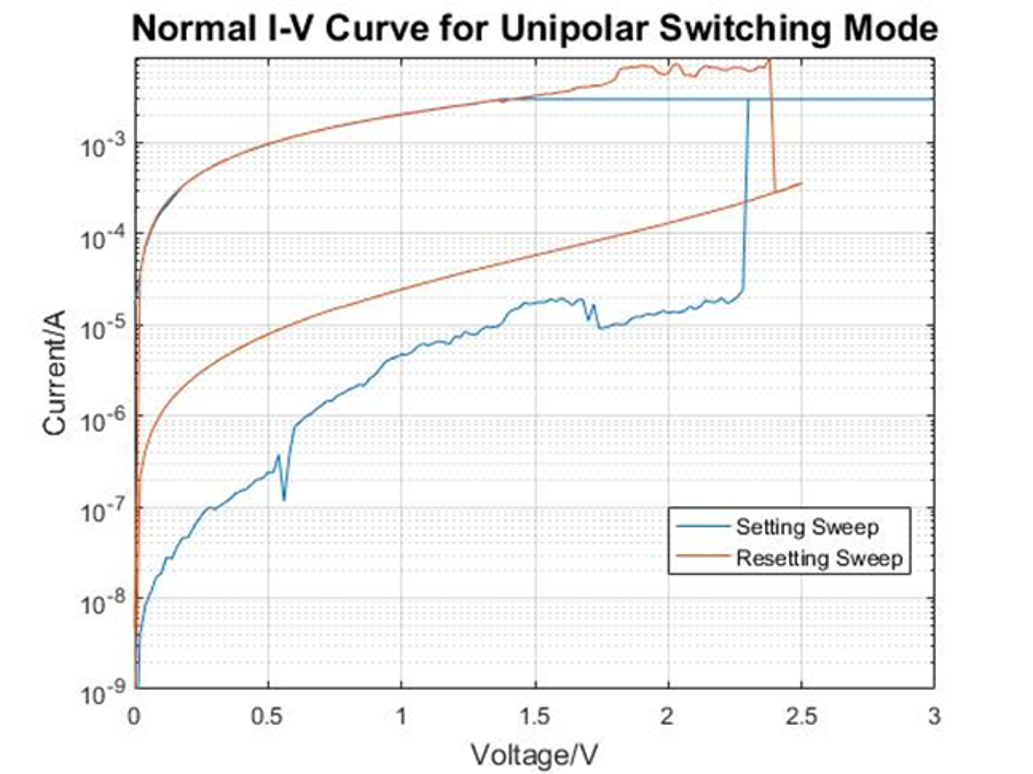
\includegraphics[width=0.6\textwidth]{Chapter3/Figs/h.png}
    \caption[Non-volatile switching behaviour for unipolar device under current compliance.]{Non-volatile switching behaviour for unipolar device under current compliance.}
    \label{fig:3h}
\end{figure}

\noindent The observed change in conductance may be attributed to structural changes occurring during the forming process, possibly resulting from a reduction step that involves the removal of oxygen from silicon oxide, thereby forming oxygen vacancies. Following the electroformation step, the LRS demonstrates stability. The device maintains its state subsequent to the removal of the electrical stimulus, thereby exhibiting non-volatile switching characteristics. It is important to note that the initial very HRS is never recovered. \\

\noindent As demonstrated in Figure \ref{fig:3h}, the unipolar switching mechanism is evident in the initial set of symmetrical MIM devices. The blue plot indicates the Set process, whereby the device transitions from the "Off" state to the "On" state at a specific threshold voltage, approximately 2.3V in this instance. \\

\noindent In this instance, the sweeping voltage has been configured to 3V with 3 mA current compliance, a setting sufficient for the switching process to occur. It has been demonstrated that a reduction in voltage below the threshold does not result in the device transitioning to its previous state.\\

\noindent It is evident that a critical current must be attained for the purpose of resetting the device. The Reset process can be observed in the orange plot, which displays a larger current, approximately one order of magnitude greater than the setting current compliance. This results in the device being restored to HRS. \\

\noindent The phenomenon of Joule heating is induced by high-current flow, resulting in localised heating and device reset. In the absence of current compliance, the device may undergo a hard breakdown or exhibit multiple transitions between the two states. It is important to note that the switching sequence can be performed repeatedly.\\ 

\begin{figure}[htbp!] 
    \centering    
    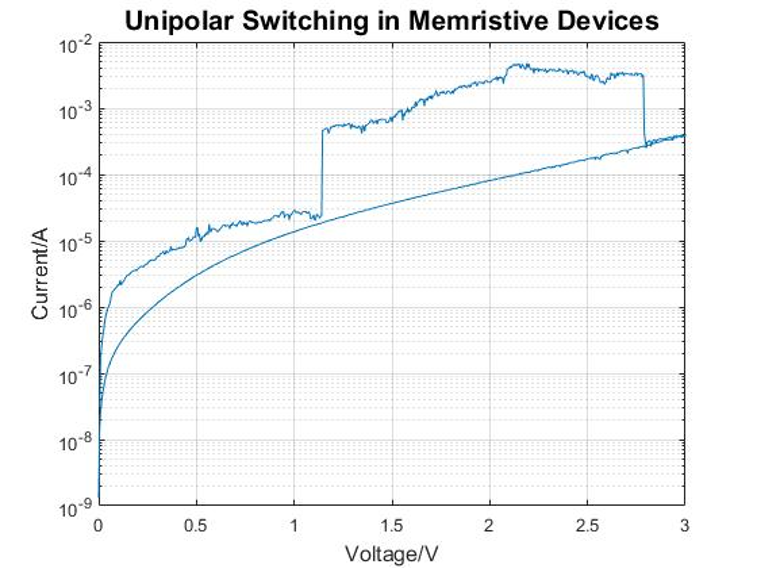
\includegraphics[width=0.6\textwidth]{Chapter3/Figs/i.png}
    \caption[Observation of Set and Reset process under the same sweep.]{Observation of Set and Reset process under the same sweep.}
    \label{fig:3i}
\end{figure}

\noindent The HRS conductance remains in a state between that of the LRS and the pristine state. In both cases, the transition is found to be abrupt and independent of the sweeping parameters, in contrast to the ideal pinched hysteresis loop suggested in the previous chapter. In summary, an elevated magnetic field is likely to set the device in the LRS, whereas high Joule heating is likely to reset the device to the HRS.\\


\noindent An alternative mechanism for unipolar switching can be observed in Figure \ref{fig:3i}. Devices with a setting voltage lower than the reset voltage will transition to LRS at a lower voltage. Subsequently, these devices will return to HRS at a higher voltage, which in this case is 1.15V and 2.85V, respectively. There is no current compliance requirement for this type of unipolar switching with reset occurring when the current has reached a critical value. \\

\begin{figure}[htbp!] 
    \centering    
    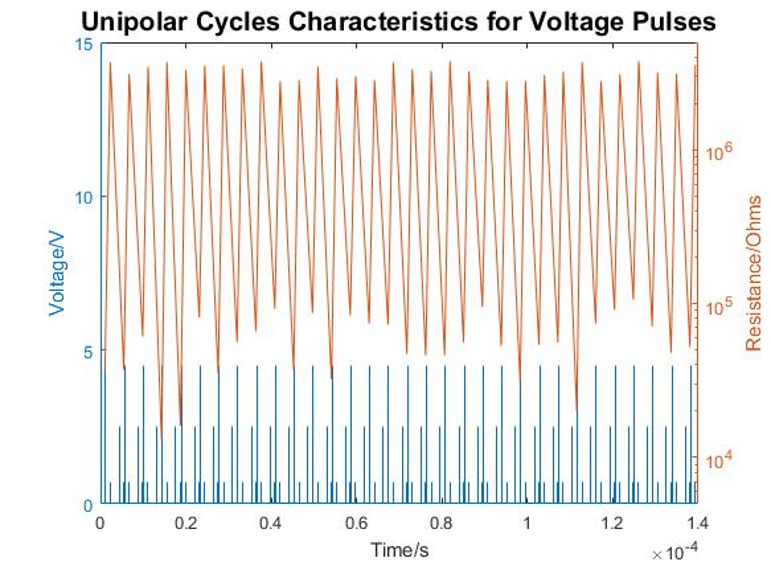
\includegraphics[width=0.6\textwidth]{Chapter3/Figs/j.png}
    \caption[Cycling stress test for unipolar device.]{Cycling stress test for unipolar device.}
    \label{fig:3j}
\end{figure}

\noindent As illustrated in Figure \ref{fig:3j}, the unipolar device undergoes cycling under conditions of stress testing. The blue spikes in the diagram represent voltage pulses that are utilised to switch the devices in positive bias. The device is set using a short voltage pulse of 4.5 V, with a duration of 100 ns. In order to effect a reset of the device, a longer voltage pulse of 2.5 volts at 2 milliseconds was utilised in order to accommodate Joule heating. \\

\noindent It was observed that each setting and resetting pulse was succeeded by a subsequent reading pulse of 0.7 V at 1 ms. The amplitude of this reading pulse is sufficiently small to avoid interfering with the set and reset process, while providing a clear reading that can be seen in the orange plot. It is evident that under typical operating conditions, the cycling resistance readings exhibit a discrepancy that is at least two orders of magnitude apart.\\

\begin{figure}[htbp!] 
    \centering    
    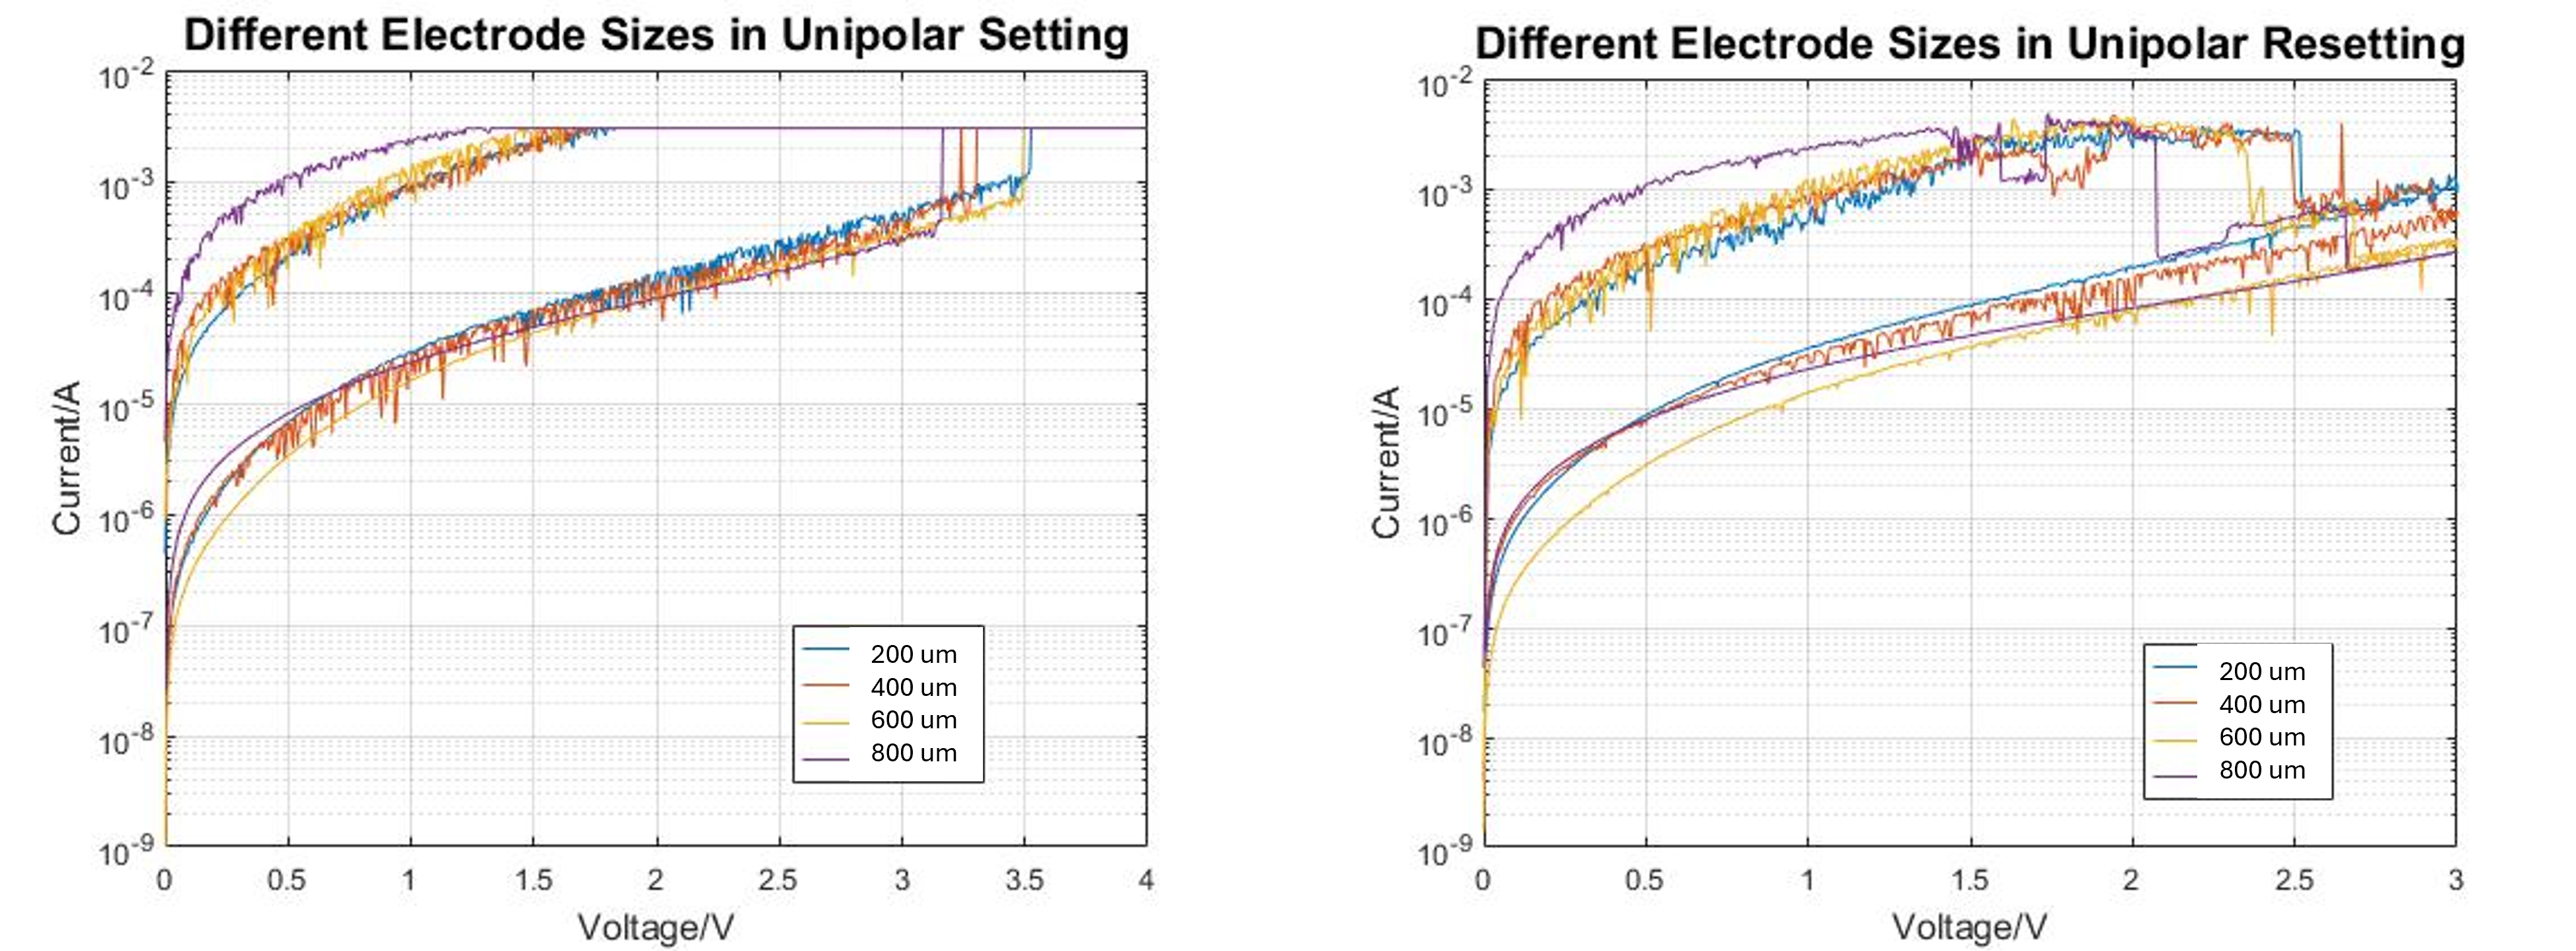
\includegraphics[width=1\textwidth]{Chapter3/Figs/k.png}
    \caption[Switching in unipolar devices across different electrode sizes.]{Switching in unipolar devices across different electrode sizes.}
    \label{fig:3k}
\end{figure}

\noindent It was also demonstrated that switching in unipolar devices is independent of electrode size. Figure \ref{fig:3k} shows that the switching processes for square contacts ranging from 200 x 200 $\mu m$ to 800 x 800 $\mu m$ are comparable. The devices consistently switch at around 3.5 V and 3 mA of current compliance. Similarly, the reset process is consistent when the samples reach the critical current threshold of approximately 5 mA.

\subsection[Bipolar Switching Mode]{Bipolar Switching Mode}

\noindent  Bipolar switching results were obtained from a set of asymmetric devices with Mo/SiOx/TiAu construct. As with unipolar devices, asymmetric bipolar devices require an initial electroforming step before the samples can be cycled between two distinct states. Figure \ref{fig:3l} shows the electroforming process in bipolar devices. A dual voltage sweep is applied to the sample up to -10 V at a current compliance of 0.1 mA. As with the unipolar devices, the sample exhibits some unstable spiking activity as the voltage sweeps from a pristine HRS to a LRS.\\


\begin{figure}[htbp!] 
    \centering    
    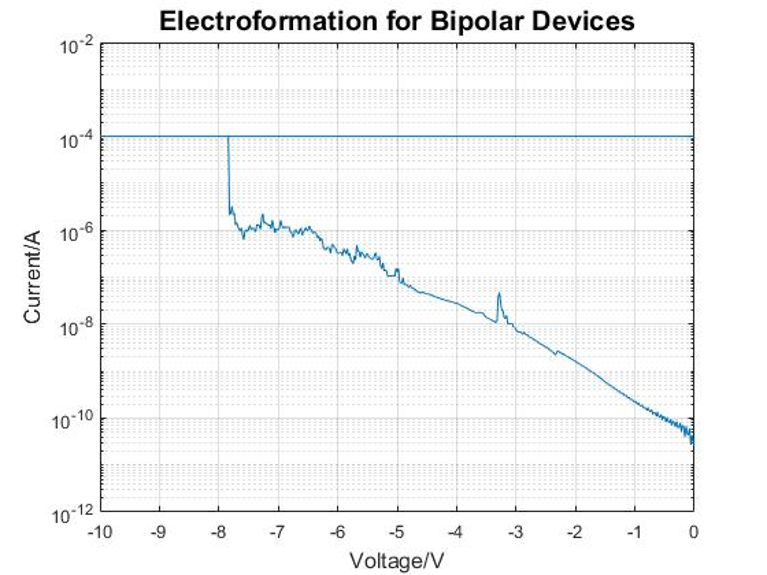
\includegraphics[width=0.6\textwidth]{Chapter3/Figs/l.png}
    \caption[Initial electroformation step for unipolar sample via a double sweep curve.]{Initial electroformation step for unipolar sample via a double sweep curve.}
    \label{fig:3l}
\end{figure}


\noindent Following the conclusion of the preliminary electroforming process, the apparatus is capable of reliably transitioning between two stable states. As illustrated in Figure \ref{fig:3m}, the device transitions between two distinct resistance states through the application of voltage stimuli of opposite polarity. The device is set using a negative voltage sweep up to -2V. \\

\begin{figure}[htbp!] 
    \centering    
    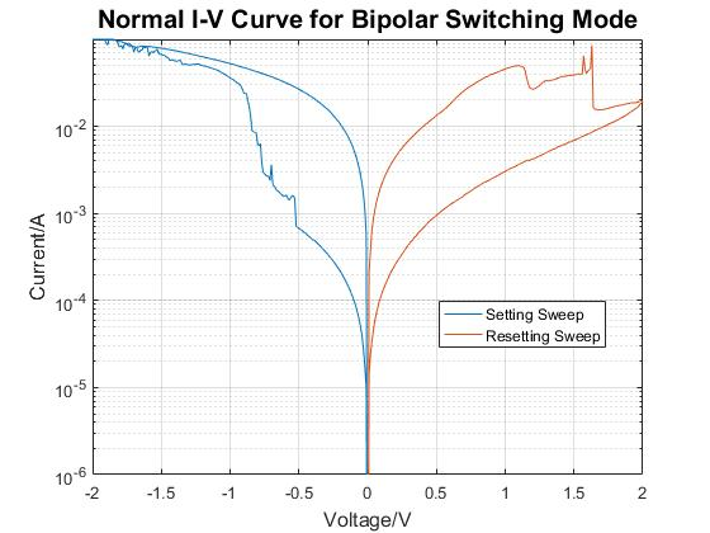
\includegraphics[width=0.6\textwidth]{Chapter3/Figs/m.png}
    \caption[Observation of bipolar switching in asymmetric device with -2V Set and 2V Reset sweeps.]{Observation of bipolar switching in asymmetric device with -2V Set and 2V Reset sweeps.}
    \label{fig:3m}
\end{figure}

\noindent The current compliance was set at 100mA in order to demonstrate a clear transition between the two states, with the conductance changing by two orders of magnitude. It is important to note that a reduced current compliance should be employed in order to achieve a balance between the device's lifespan and its conductivity. The device is reset by means of an opposing 2V dual sweep of positive polarity, a process known as bipolar switching.\\


\noindent From a physical perspective, this particular type of bipolar switching mechanism is intrinsic and can be categorised as belonging to the valence change mechanism class. In this category of memory devices, the electroforming process typically leads to local reduction, thereby forming a conductive pathway. It is hypothesised that this channel is composed of oxygen vacancies, which permit oxygen ions to migrate in and out of the channel in response to an applied electric field. \\


\noindent The location of the local redox process is hypothesised to be in proximity to a filament-to-electrode interface. The effective tunnelling barrier height at this interface is indicative of the resistance state of the device. The height of this barrier is subject to variation under different applied voltage biases, thereby inducing the movement of oxygen ions and resulting in a corresponding alteration to the resistance state. \\

\begin{figure}[htbp!] 
    \centering    
    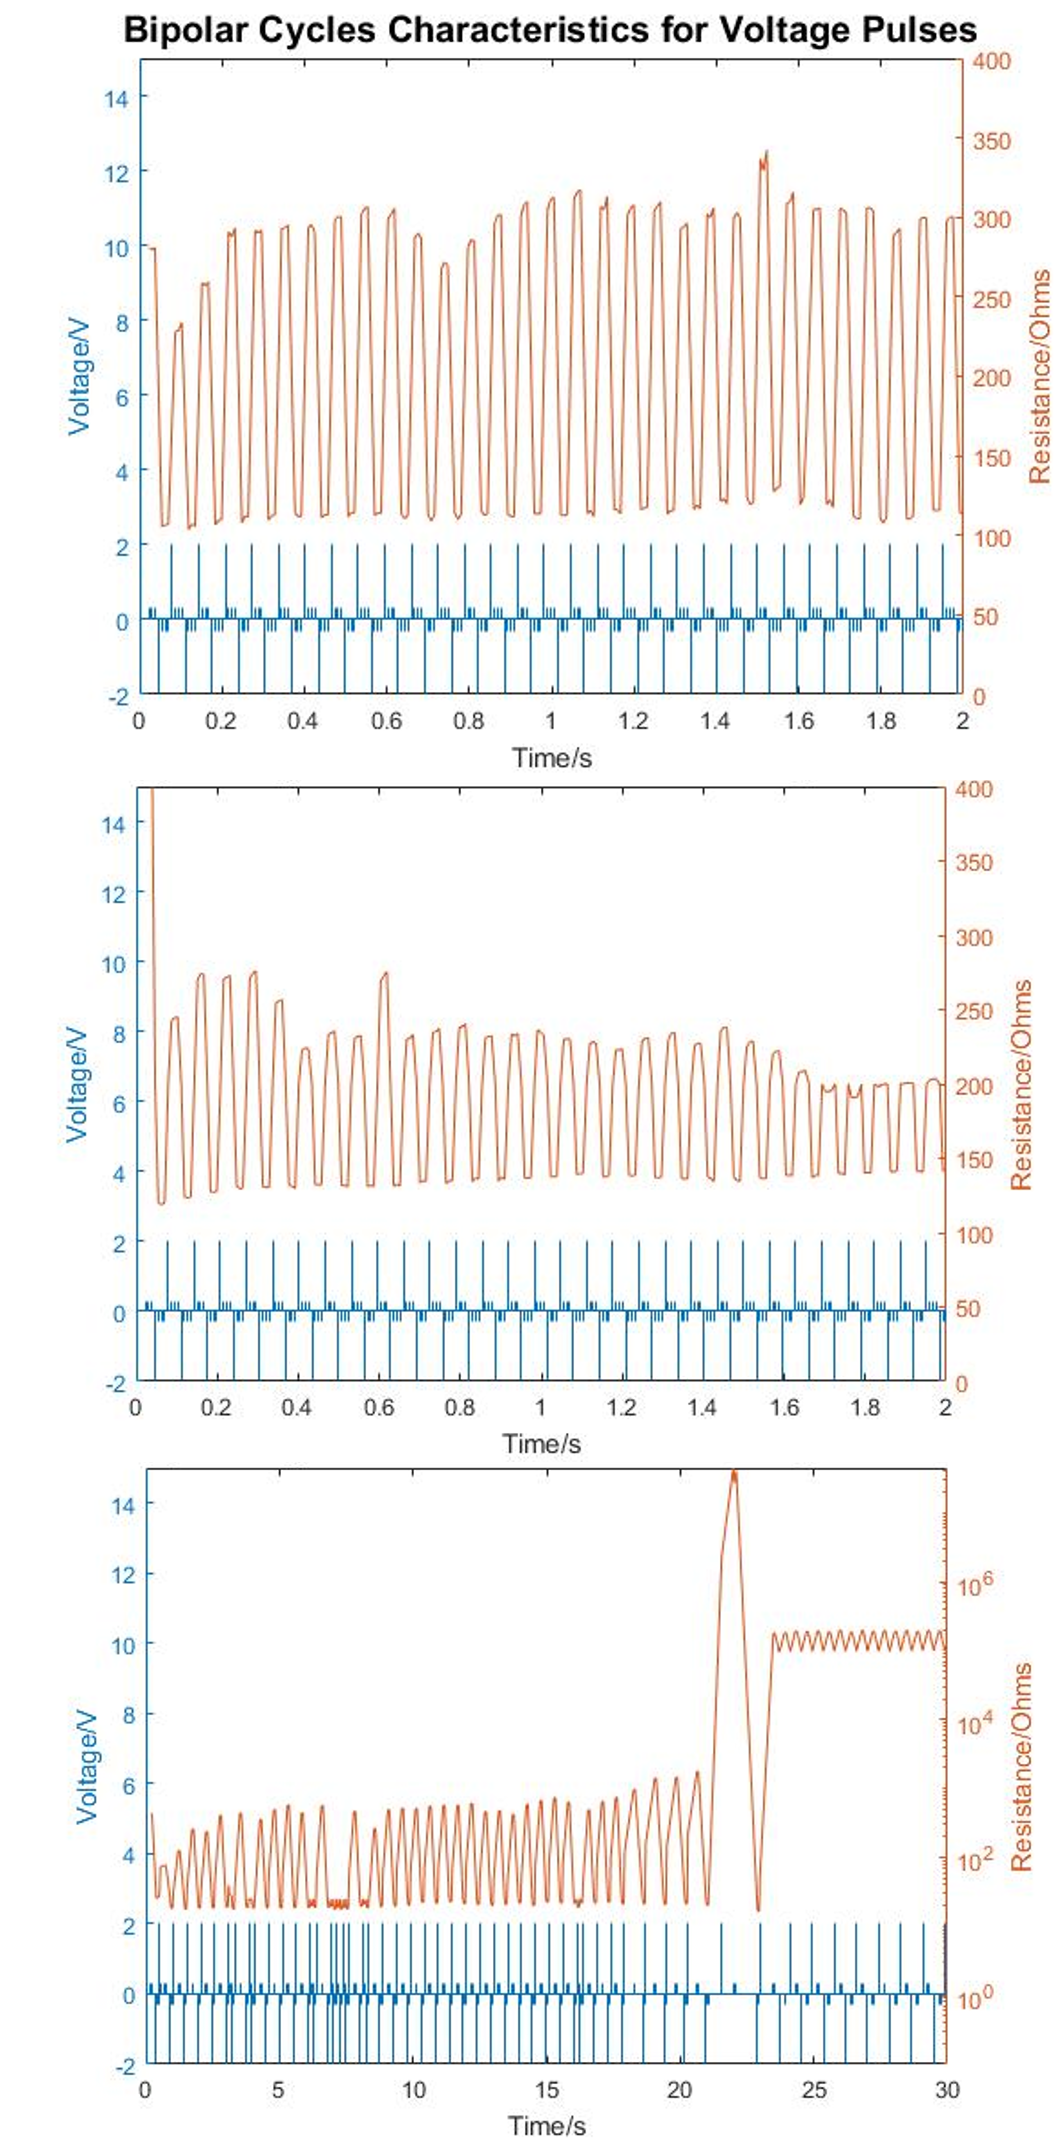
\includegraphics[width=0.65\textwidth]{Chapter3/Figs/n.png}
    \caption[Cycling stress test for bipolar devices.]{Cycling stress test for bipolar devices. Initial device cylcles (top) followed by LRS convergence (middle) and hard reset breakdown (bottom).}
    \label{fig:3n}
\end{figure}

\noindent The transition between these two resistive states can be facilitated by the application of suitable voltage pulses. As demonstrated in Figure \ref{fig:3n}, the device exhibits a high degree of reliability in its switching capability when utilising a -2 V setting, in conjunction with 2 V resetting pulses. \\


\noindent It was recorded that each setting or resetting pulse is succeeded by five 0.1V or 0.1V reading pulses for the resistive state that the device is purportedly in. In this configuration, the HRS is approximately 300$\Omega$, while the LRS is about 100 $\Omega$. It is noteworthy that the selection of these voltage pulses was made with the objective of accurately measuring the resistance, without causing the switching mechanisms of the device to be triggered.\\

\noindent In the experiment, the device demonstrated a minimum of 4500 cycles of operational longevity when subjected to a current bias of 10mA. This was followed by a convergence towards LRS, as evidenced by the switching between 200$\Omega$ and 150$\Omega$, as depicted in Figure \ref{fig:3n}. As an alternative scenario, when the device is operating at a higher current compliance of 100mA, the stress test sustains approximately 40 cycles before the device experiences irreversible failure, entering the HRS state at 200k$\Omega$. \\


\noindent Finally, Figure 35 demonstrates switching behaviours for bipolar devices across a range of contact sizes, from 200 x 200$\mu m$ to 800 x 800$\mu m$. All the setting sweeps were programmed up to -2V with 5mA current compliance for the purpose of facilitating clear transition observation. It is evident that the resetting sweep has been configured to a voltage of 2V, with a current compliance of 100mA. \\

\noindent The results obtained demonstrate some variations in the switching voltages and contrast ratio between HRS and LRS. This finding suggests the potential necessity for further statistical analysis in subsequent devices. However, it is evident that all samples demonstrate consistent switching activities within the range of voltage stimuli applied during the testing process.

\begin{figure}[htbp!] 
    \centering    
    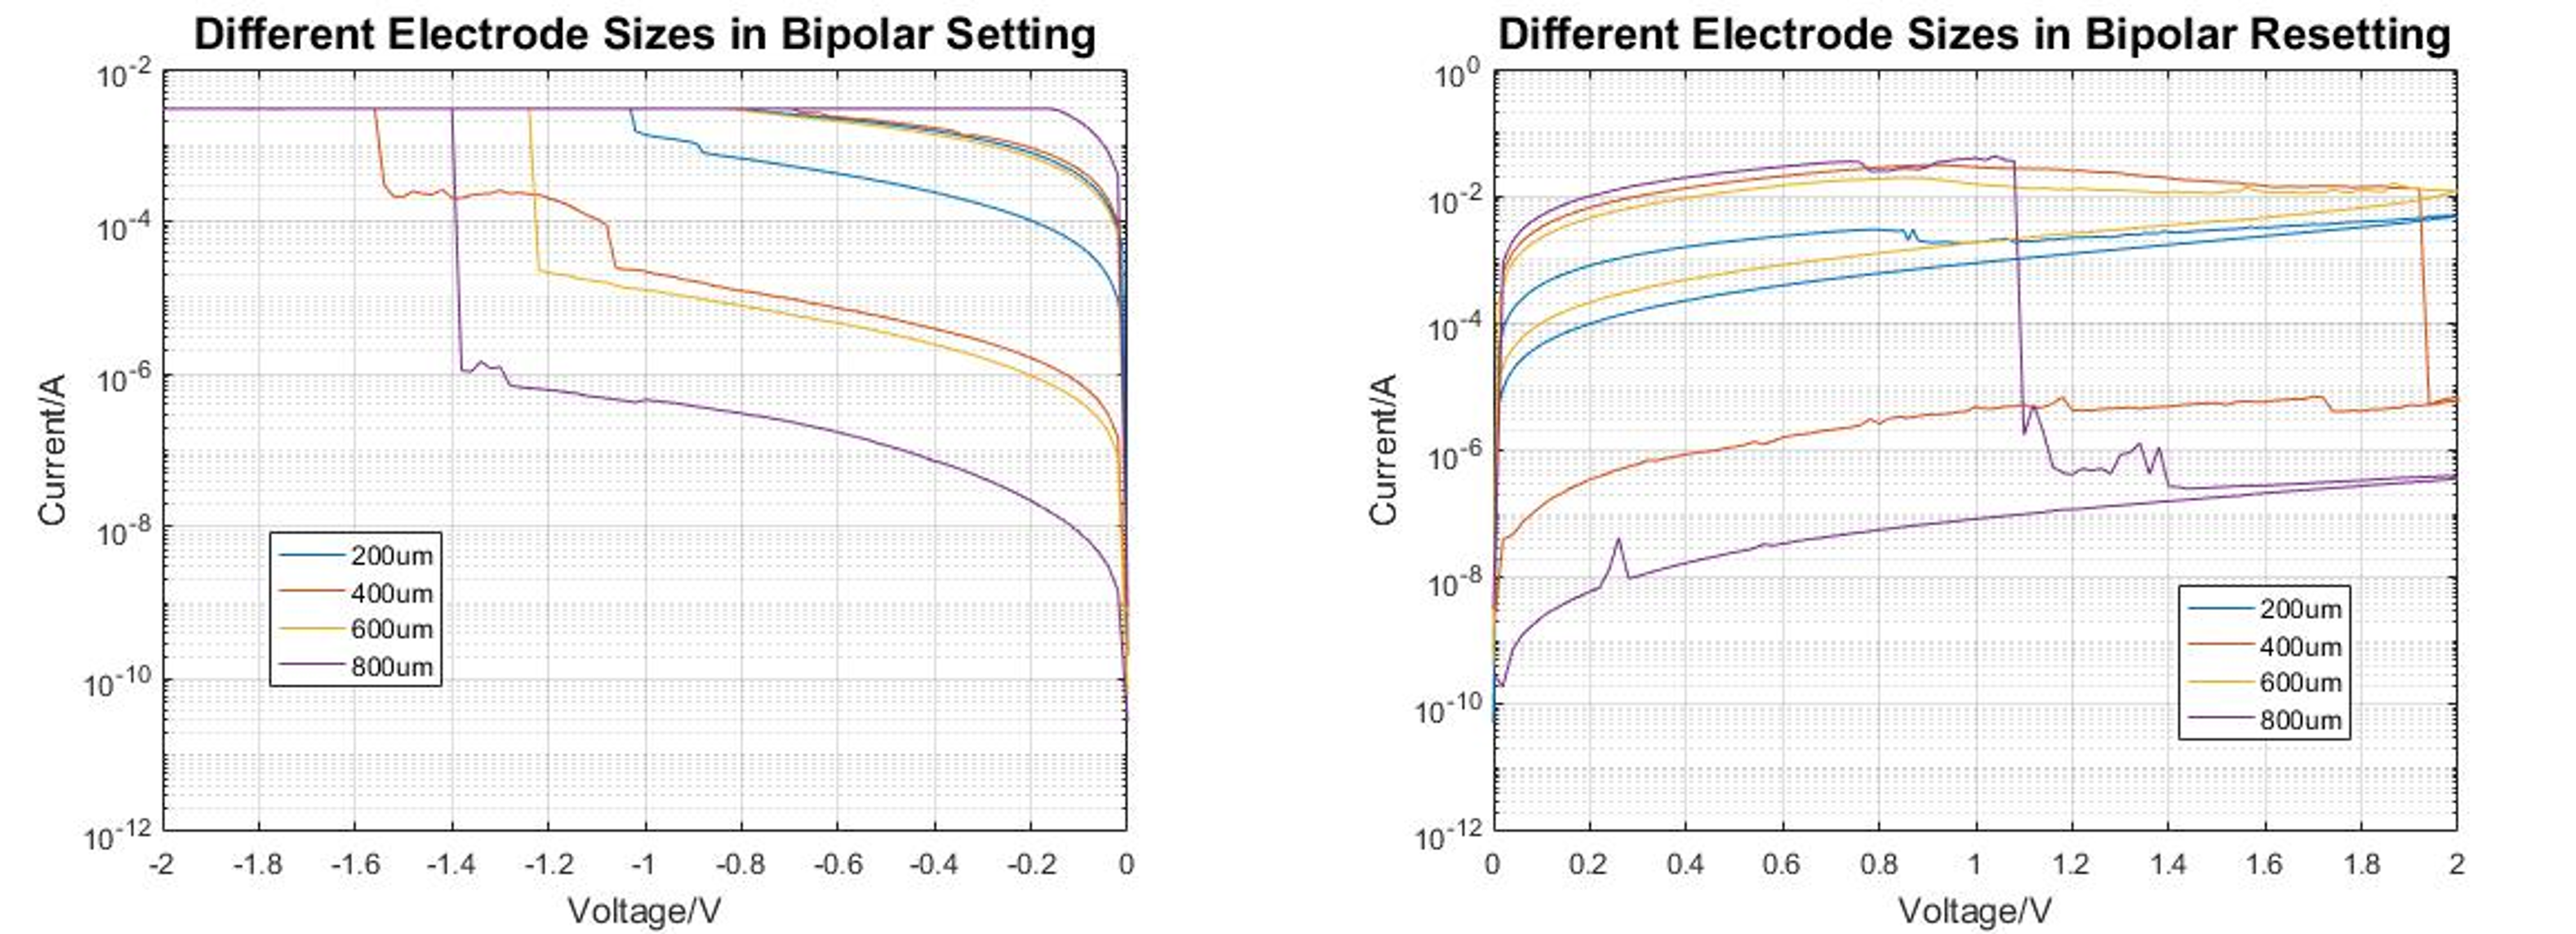
\includegraphics[width=1\textwidth]{Chapter3/Figs/o.png}
    \caption[Switching in bipolar devices across different electrode sizes.]{Switching in bipolar devices across different electrode sizes.}
    \label{fig:3o}
\end{figure}

\subsection[Alternate Operating Modes]{Alternate Operating Modes}

As demonstrated in previous observations, the switching of both unipolar and polar samples is reliable under specific, correctly configured, programming conditions. Furthermore, it appears that the switching does not scale in proportion to the electrode contact size. This finding indicates that carrier transport occurs for individual conducting filaments. However, it should be noted that certain devices exhibit alternative switching modes, namely gradual and multi-level switching modes. The presence of parallel conductive pathways within the same insulating layer is a potential cause of this phenomenon. \\

\begin{figure}[htbp!] 
    \centering    
    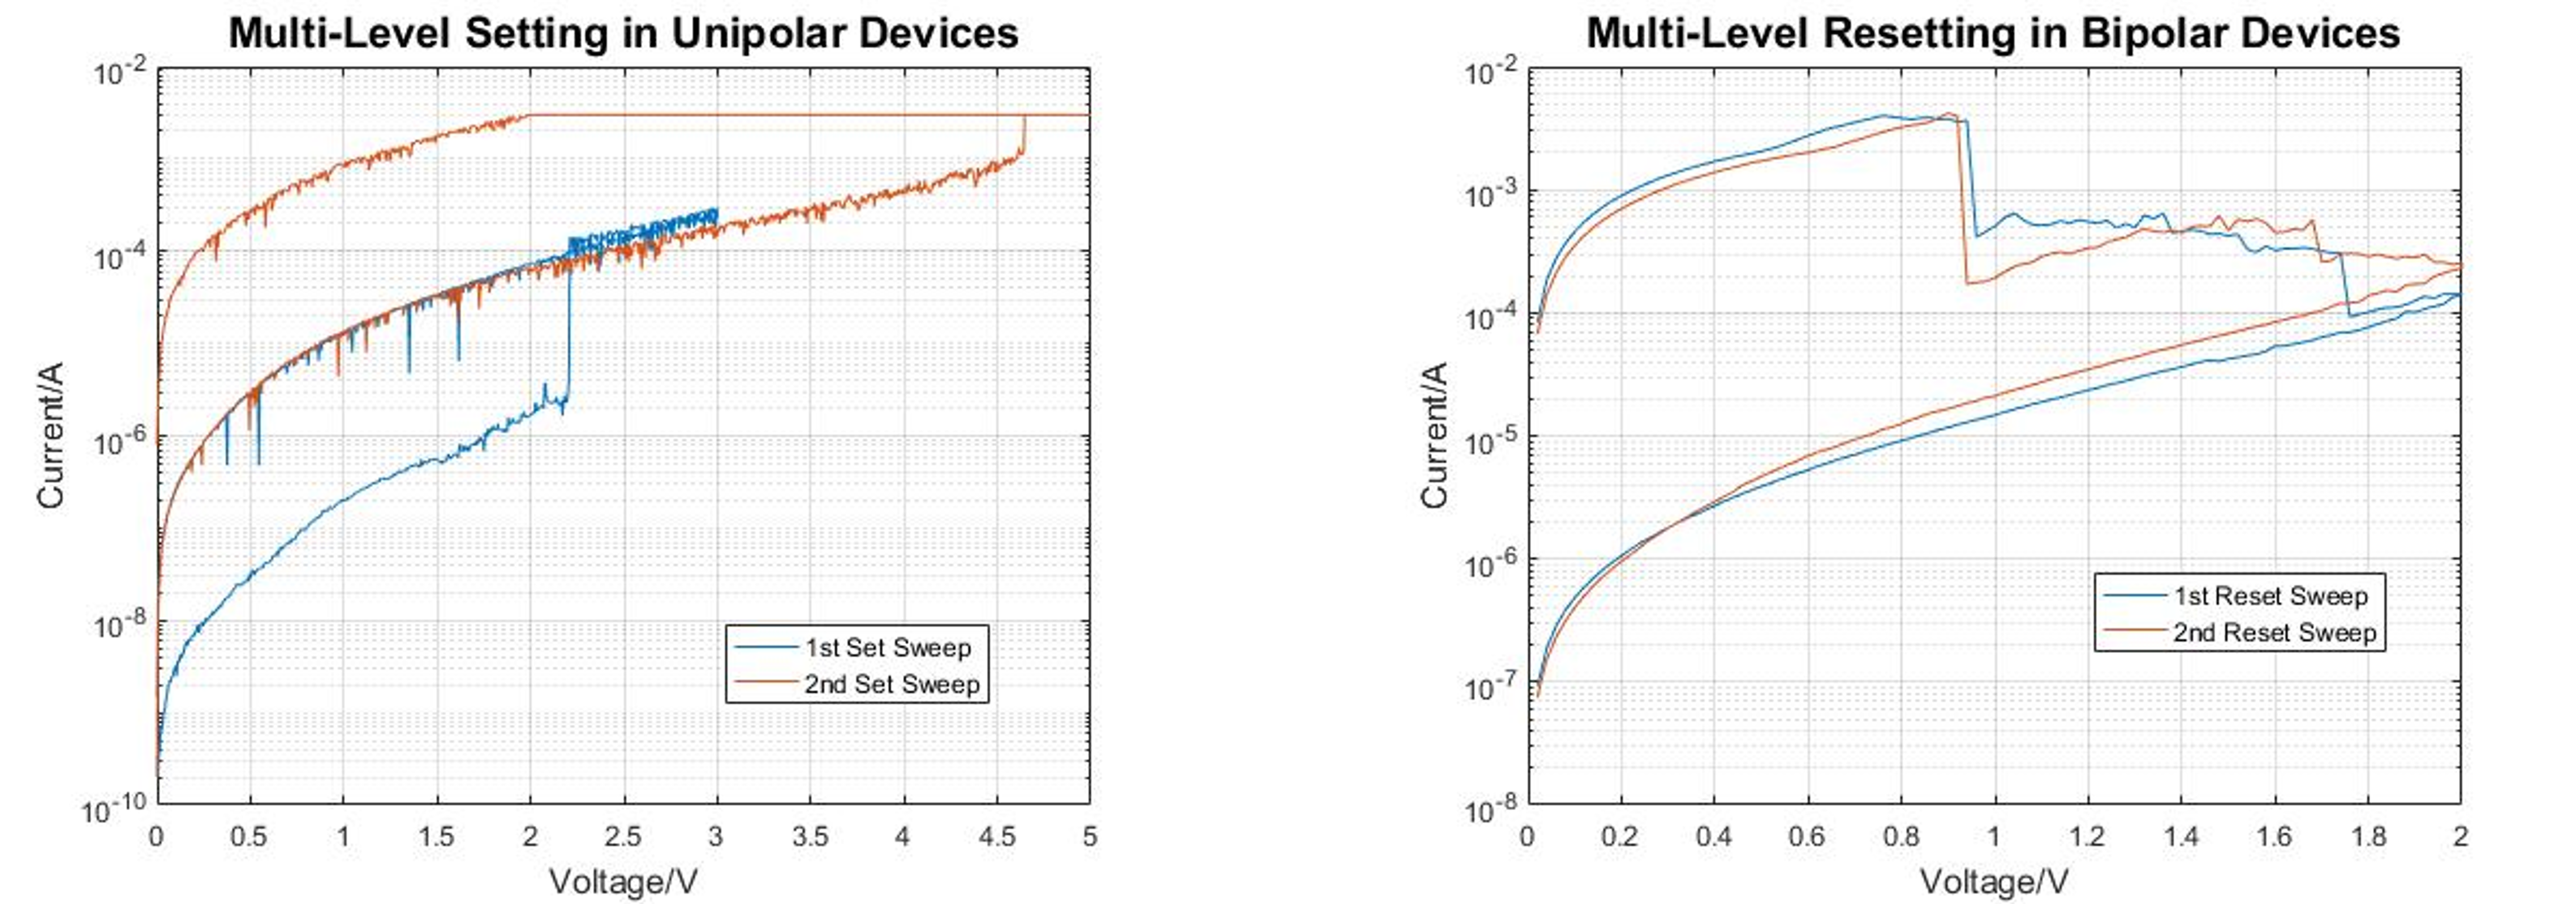
\includegraphics[width=1\textwidth]{Chapter3/Figs/p.png}
    \caption[Multi-levels I-V characteristics in MIM devices.]{Multi-levels I-V characteristics in MIM devices during the Set (left) and Reset (right) process.}
    \label{fig:3p}
\end{figure}

\noindent In both unipolar and bipolar samples, there are some devices exhibiting the multilevel switching characteristic, as illustrated in Figure \ref{fig:3p}. The initial transition process during the set stage can be followed by a subsequent stable transition to an even lower LRS, thereby providing a minimum of three or more switchable states. \\

\noindent As demonstrated above, both setting states are found to be stable, with the HRS of the second sweep coinciding with the LRS of the first sweep. The device can be configured at the first or second LRS, with two separate voltage sweep levels available for this purpose. As illustrated in the aforementioned example, the generation of the primary and secondary LRS was achieved through the utilisation of 3V and 5V sweeps, respectively.\\

\begin{figure}[htbp!] 
    \centering    
    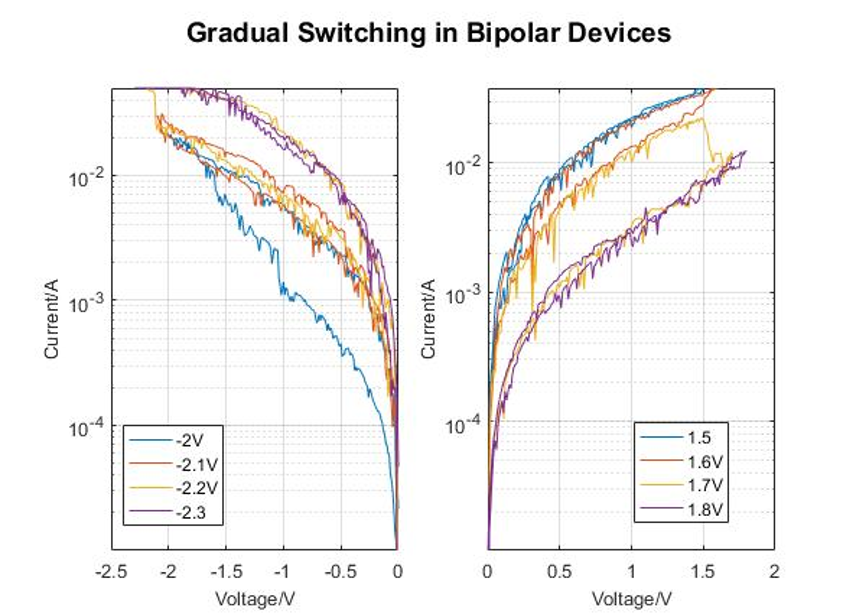
\includegraphics[width=0.7\textwidth]{Chapter3/Figs/q.png}
    \caption[Gradual increase (left) and decrease (right) in conductivity for bipolar device.]{Gradual increase (left) and decrease (right) in conductivity for bipolar device.}
    \label{fig:3q}
\end{figure}

\noindent In a similar manner, multilevel reset can be observed in bipolar samples at 1V and 1.8V, respectively. It is important to note that, in this case, the transitions window is smaller than that of the unipolar devices. In both cases, the switching is stable, with a contrast ratio between each state that is at least one order of magnitude.\\

\noindent In the case of bipolar switching samples, it is possible to observe not only the abrupt changes in resistance that are normally observed, but also gradual changes in conductivity (see Figure \ref{fig:3q}). As indicated by HRS, the gradual increase in conductance is achieved by sequentially sweeping the device with increasing setting voltage levels, ranging from -2V to -2.3V, under an appropriate stepping current compliance of 100mA in this case.\\

\noindent It has been demonstrated that a gradual decrease in conductivity is generated during the reset process, with this decrease commencing from LRS. This gradual change is obtained by progressively sweeping the device at higher potential, from 1.5V to 1.8V. The concluding phase of these procedures is characteristically sudden, thereby impeding the attainment of further transitions. The outcomes obtained were found to vary in terms of their gradualness or abruptness, suggesting the potential for further statistical analysis with reduced voltage steps in subsequent characterisations.\\

\begin{figure}[htbp!] 
    \centering    
    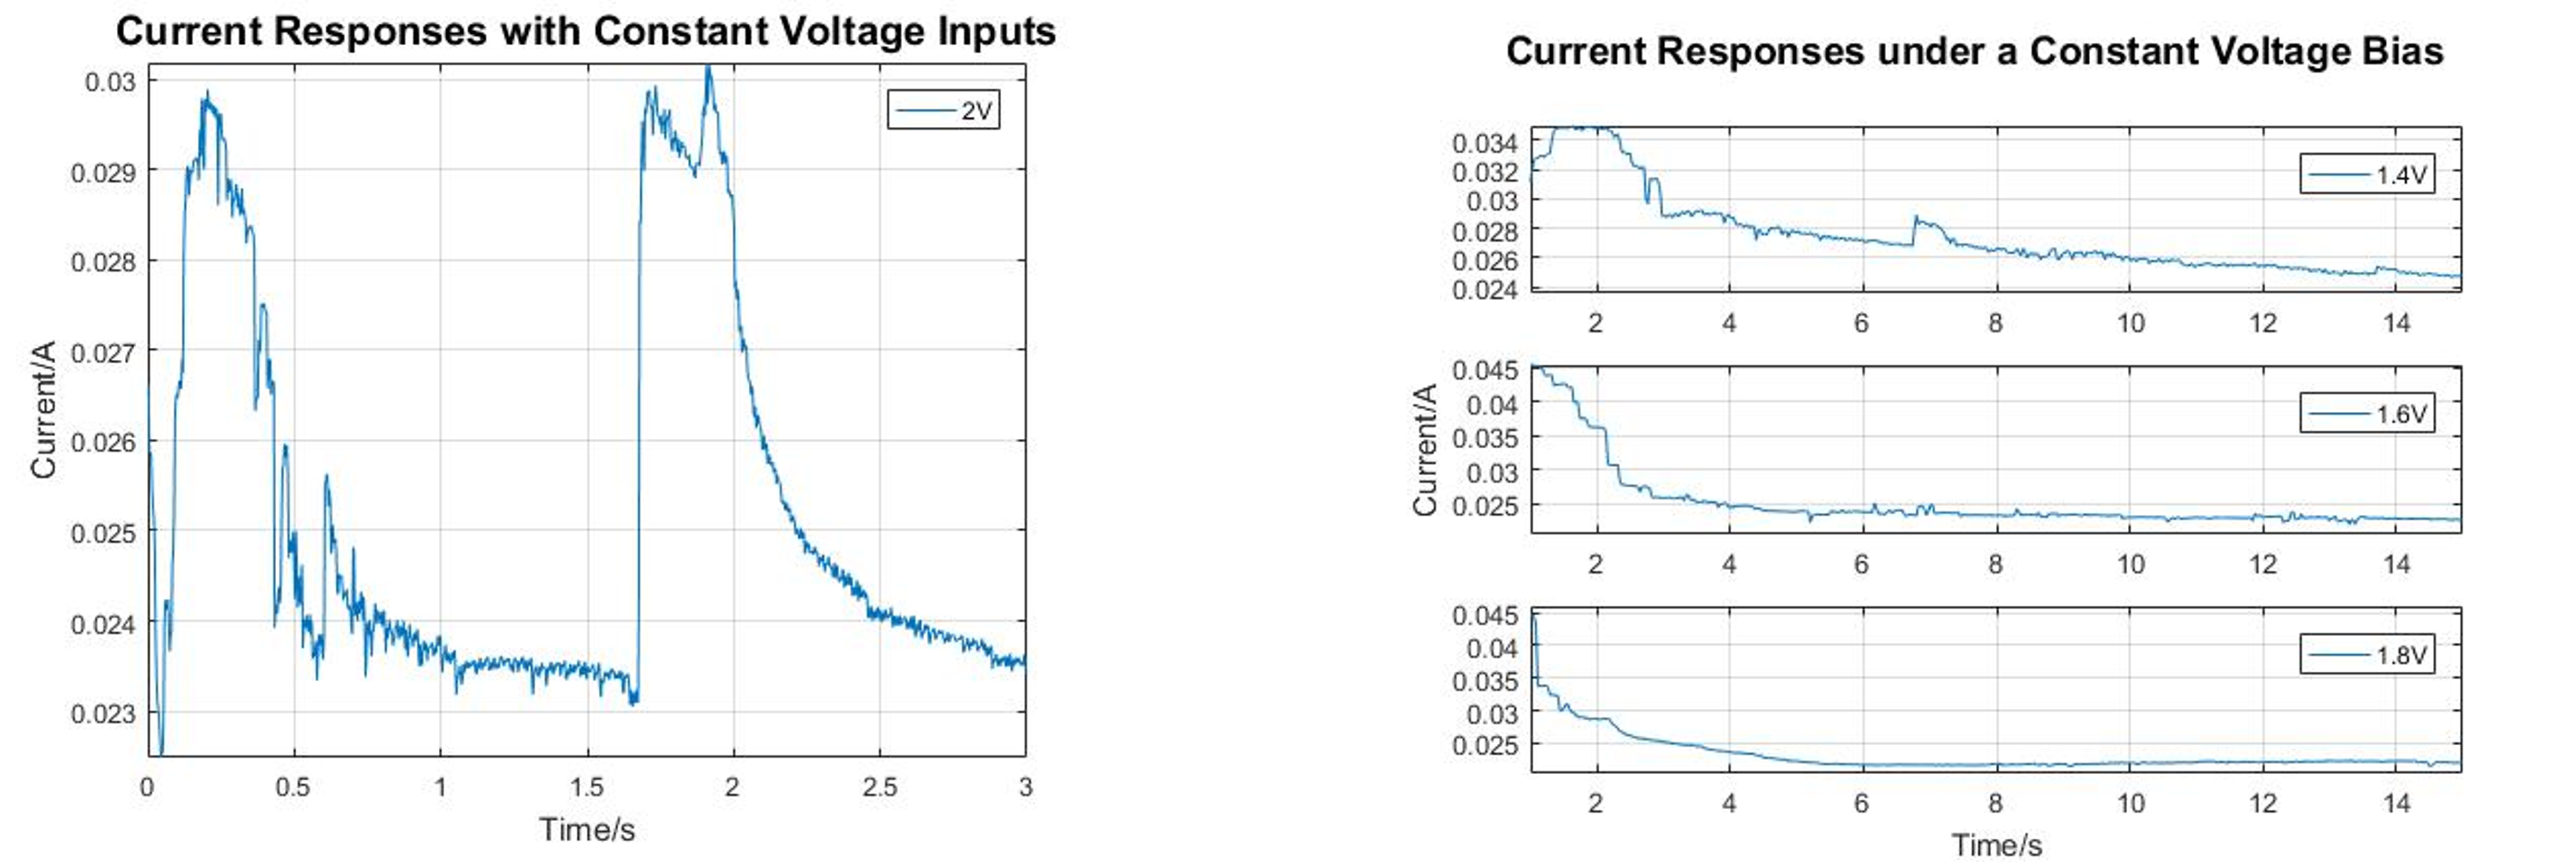
\includegraphics[width=1\textwidth]{Chapter3/Figs/r.png}
    \caption[Current-time plots showing transitions between resistive states.]{Current-time plots showing transitions between resistive states (left) and time constant comparison (right).}
    \label{fig:3r}
\end{figure}

\noindent As information processing is concerned with the manner in which data is processed over time, it is imperative to assess the performance of devices over time. In the preceding section, the switching mechanisms have been investigated with regard to time via the cycling stress tests. In this experiment, the characteristics of the device under constant voltage and current bias will be observed.\\

\noindent As illustrated in Figure \ref{fig:3r}, the current time plot for different voltage biases in unipolar samples is demonstrated. Applying a voltage of 2V to the device results in discernible transitions between the set and reset processes, with these transitions exhibiting an inverse relationship to one another. \\

\noindent It is evident that alterations in the resistive state can be observed when there is a rapid increase in the current (set), which is then shortly followed by an exponential decay (reset). The rate of recovery is indicated by the time constant of the exponential decay. A comparison of the individual inputs reveals that the time constant varies in proportion to the voltage bias. When the voltage bias increases from 1.4V to 1.8V, the time constant decreases from 7s to 1s.\\

\begin{figure}[htbp!] 
    \centering    
    \includegraphics[width=1\textwidth]{Chapter3/Figs/s.png}
    \caption[Volatile activities observed under different constant current inputs.]{Volatile activities observed under different constant current inputs for unipolar device (left) and switching at sufficiently high input current bias in bipolar device (right).}
    \label{fig:3s}
\end{figure}

\noindent When a constant current is applied to the samples, volatile spiking activities can be observed in Figure \ref{fig:3s}. It is evident that an increase in current from $5\mu A$ to $10 \mu A$, as observed for unipolar devices, results in a corresponding rise in volatility. This phenomenon can be attributed to the constant current input, which has a significant impact on the device's response. These instabilities can manifest as amplitude variations, with spikes ranging from 0.02V to 0.45V, or as timing variations, with spikes occurring more frequently at higher current biases.\\

\noindent The device exhibits spiking activities until the current bias is sufficiently large to trigger a switching transition. When the bipolar device is critically biased at -10mA, it switches shortly after exhibiting volatile activities, following an uncharacteristically large spike. Following the transition, the spiking behaviours become less predominant.

\section[Resistive Switching in Silicon Oxide]{Resistive Switching in Silicon Oxide}

\noindent The present section aims to propose a phenomenological model that governs the switching activities in silicon-rich silica of RRAM devices. The model under discussion will be based on the theory obtained from the literature review in the preceding chapter, with a particular emphasis on the distinction between unipolar and bipolar modes of switching. \\

\noindent  In the context of oxide ReRAM devices, two commonly employed switching settings are identified: unipolar and bipolar mode \cite{zhuge2013advances}. In the context of unipolar switching, it is notable that the alteration in resistance state is independent of the electrical stimuli polarity. The configuration of these devices is typically characterised by a symmetrical design, incorporating electrodes of equal dimensions on both the top and bottom surfaces. \\

\noindent The present compliance is utilised for the purpose of averting any impairment to the device that may be occasioned by a hard breakdown during the switching process.  Conversely, bipolar devices necessitate the application of electrical stimuli of contrasting polarity to execute switching operations.

\subsection[Conduction Mechanisms]{Conduction Mechanisms}

\noindent For the devices and samples referenced in this study, the primary material utilised for the insulating layer is silicon dioxide, $SiO_x$. It has been reported that silicon dioxide has been doped with conducting ions, such as silver or copper, during the fabrication process in order to behave like ECM cells. \\

\noindent However, diffusion of metallic ions is generally undesirable in CMOS processing, as it can compromise the operations of neighbouring electronics. The present study is concerned with the intrinsic resistive switching property, irrespective of the electrode materials. Given that silicon-rich silica is predominantly employed in the insulating layer, its capacity for complete CMOS-compatible processing is deemed to be highly favourable. \\

\begin{figure}[htbp!] 
    \centering    
    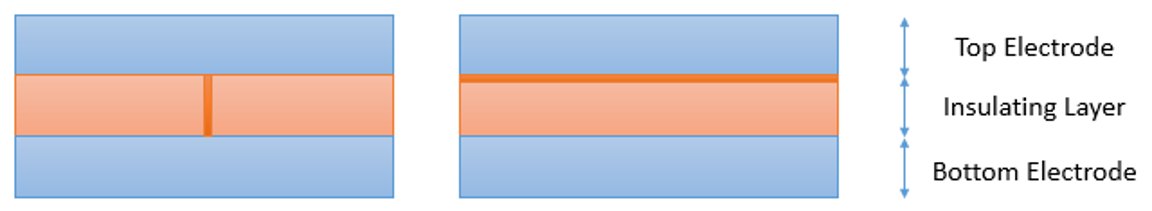
\includegraphics[width=1\textwidth]{Chapter3/Figs/t.png}
    \caption[: Conductive regions for filamentary switching and interface switching.]{: Conductive regions for filamentary switching (left) and interface switching (right).}
    \label{fig:3t}
\end{figure}

\noindent In the context of bulk silicon oxide, the formation of a conductive filament within the insulating layer typically occurs during the electroforming process. This conductive filament is generally independent of electrode size, with the switching mechanism being dominated by a single filament. The switching process instigates a minor alteration to the filament. It has been established that this is independent of the insulating layer thickness. This is due to the fact that changes in resistance usually take place in a localised region.\\

\noindent The surface switching mechanism is comparatively under-researched in comparison to filamentary switching. The conductivity of this mechanism is found to be predominantly contingent upon the dimensions of the electrode. The primary driving force behind this mechanism is the formation of a Schottky tunnel barrier across the entire electrode interface and the insulating layer. Consequently, a switching layer is formed at the interface.\\

\begin{figure}[htbp!] 
    \centering    
    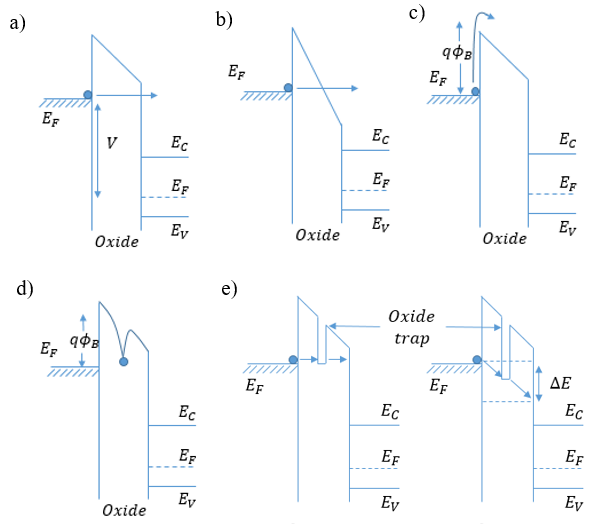
\includegraphics[width=0.65\textwidth]{Chapter3/Figs/u.png}
    \caption[Energy-band diagrams showing different conduction mechanisms.]{Energy-band diagrams showing different conduction mechanisms: (a) direct tunnelling, (b) Fowler-Nordheim tunnelling, (c) thermionic emission, (d) Poole-Frenkel emission, (e) trap-assisted tunnelling \cite{sze2021physics}}
    \label{fig:3u}
\end{figure}

\noindent Electrical conductivity is defined as an intrinsic property that determines the extent to which a given material can oppose a flow of charge. The ideal insulator is characterised by a complete absence of conductance and infinite resistance. It is evident that the conductivity of the silicon oxide thin film, which is measured in several hundred nanometres, is suboptimal due to the presence of a finite amount of conductance. The conductivity of the semiconductor material is also contingent on a variety of external conditions. The aforementioned parameters encompass specific frequencies of light, temperature dependency and applied electric field.
\begin{align}
    E = \frac{V}{d} \label{eq:3.1}
\end{align}

\noindent In  (\ref{eq:3.1}), the electric field strength, E, can be expressed as a function of the applied voltage, V, and the distance that the voltage is being applied across, d. Nevertheless, it is important to note that this fundamental estimate may not be applicable to the actual devices. The validity of assumptions regarding negligible oxide charges, voltage flat-band and small band bending may be called into question. In order to facilitate a more thorough analysis and identification of the switching procedure in the samples, additional conduction mechanisms in the insulator are considered.
\begin{align}
    J &\propto E^{2} exp\left[ -\frac{4\sqrt{2m^{*}}(q\phi _{B})^{^{3/2}}}{3q\hslash E_{i}} \right] \label{eq:3.2} \\
    J &\propto V^2exp \left( -\frac{b}{V}\right) \label{eq:3.3}
\end{align}

\noindent (\ref{eq:3.2}) displays the tunnelling current density's dependence on the electric field and voltage, applied as appropriate, while being independent of temperature. In the context of the aforementioned equation, $\phi_B$ denotes the tunnelling barrier height, E represents the insulator electric field, $m^*$ is defined as 0.42m, which is the carrier effective mass for silicon oxide, $\hslash$ is the reduced Planck constant, $q$ is the electric charge, and $b$ is a constant of proportionality.\\

\noindent In the presence of a strong electric field, conventional tunnelling is the predominant conduction mode for insulating materials. The tunnelling process is a consequence of quantum mechanical effects, with the electron wave function having a finite probability of penetrating through a potential barrier of finite height. Conventional quantum tunnelling refers to the direct passage of an electron through the entire width of a barrier. Alternatively, Fowler-Nordheim tunnelling refers to the electron tunnelling through only part of this height.
\begin{align}
    J &\propto E \cdot exp\left( -\frac{\Delta E_a}{kT} \right) \label{eq:3.4} \\
    J &\propto \frac{V}{T} \cdot exp \left( -\frac{c}{T}\right) \label{eq:3.5}
\end{align}

\noindent (\ref{eq:3.4})  illustrates the ohmic current density as a function of electric field, as well as the voltage applied and the temperature. In this equation, $\Delta E_a$ denotes the activation energy, $k$ is the Boltzmann constant, $T$ is the temperature in Kelvin and $c$ is a constant of proportionality. In the context of low fields and elevated temperatures, ohmic conduction exerts a predominant influence. This phenomenon entails the thermally induced excitation of carriers, thereby facilitating their transition between conductive states.
\begin{align}
    J &\propto \frac{E}{T} \cdot exp\left( -\frac{\Delta E_a}{kT} \right) \label{eq:3.6} \\
    J &\propto \frac{V}{T} \cdot exp \left( -\frac{d}{T}\right) \label{eq:3.7}
\end{align}
\noindent Ionic conduction exhibits a comparable expression to ohmic conduction, yet it possesses a distinct activation energy and constant of proportionality. This process is typically characterised by the movement of ions across a material via defects in the crystal lattice of a solid. For an ideal insulator, ions cannot readily travel into and out of the material. \\

\noindent However, an applied electric field will result in the build-up of ionic carriers at the metal-to-insulator interfaces, thereby modifying the voltage distribution across the region. The elimination of the applied electric field will result in the retention of a significant internal field, thereby enabling the flow of an ionic current until equilibrium is achieved.
\begin{align}
    J &= \frac{9\varepsilon _i \mu V^2}{8d^3} \label{eq:3.8} \\
    J &\propto V^2 \label{eq:3.9}
\end{align}

\noindent The phenomenon of space charge can be attributed to the injection of charge from the electrodes into the insulator, in the absence of compensating charges. The process involves the injection of charges into the dielectric from one electrode and their subsequent capture by the other. The Mott–Gurney law is delineated in (\ref{eq:3.8}) for space charge limited current in solid and in the velocity-saturation regime accordingly. \\

\noindent In this equation, $\epsilon$ denotes the dielectric permittivity, $\mu$ is the carrier mobility, $L$ is the material thickness, and $v = \mu E$ is the electron drift velocity. This conduction mechanism is predicated on the presence of a single type of charge carrier, the absence of intrinsic conductivity, and an electric field of zero magnitude at the cathode responsible for the injection of charge.\\

\noindent Further exploration will be directed towards other conduction mechanisms, including Schottky emission and Poole-Frenkel conduction, which will be examined in greater detail. Schottky emission, otherwise known as thermionic emission, occurs when the carriers receive thermal energy in excess of the potential barrier height. The phenomenon of Poole-Frenkel conduction occurs when trapped electrons are thermally excited into the conduction band.

\subsubsection[Fowler-Nordheim Tunnelling]{Fowler-Nordheim Tunnelling}

\noindent In the presence of elevated electric fields, quantum mechanical tunnelling emerges as the predominant conduction mechanism in insulating materials. This is a consequence of the process inherent in quantum mechanics, whereby the electron wave function is capable of penetrating a potential barrier. \\

\noindent This process is typically contingent on the electric field, irrespective of temperature. The phenomenon of direct tunnelling occurs when carriers traverse the entire width of the barrier. It has been established that, in the context of Fowler-Nordheim tunnelling, carriers only traverse a proportion of this width.
\begin{align}
    J &= \frac{q^2E^2}{8\pi\hslash\phi _B} exp \left[  -\frac{4\sqrt{2m^{*}}(q\phi _{B})^{^{3/2}}}{3q\hslash E_{i}} \right] \label{eq:3.10} \\
    J &\propto \frac{4\pi q m^* kT}{\hslash^3} \label{eq:3.11}
\end{align}

\noindent The phenomenon of Fowler-Nordheim tunnelling is contingent upon the trapezoidal configuration of the potential barrier. In the presence of a substantial application of an electric field, an increased incidence of band-bending is observed. This results in a significant reduction in the effective width required for carriers to tunnel through. In the context of a thick oxide layer, this is the prevailing conduction mechanism for a metal oxide structure. Subsequent to the tunnelling process, the carriers are able to move freely between the conduction and valence bands.\\

\noindent The identification of the mechanism for the device is possible through the rearrangement of (\ref{eq:3.10}) and the graphical representation of the Fowler-Nordheim plot of $ln(J/E^2)$ against $\frac{1}{E}$ for experimental I-V characterisations. The gradient of this straight-line plot is equivalent to $-\frac{4\sqrt{2m^{*}}(q\phi _{B})^{^{3/2}}}{3q\hslash}$, which can be rearranged to obtain the barrier height $\phi_B$. The y-intercept, on the other hand, describes the geometrical efficiency of electron-field emission. The occurrence of this mechanism is contingent upon the product of the electric field and layer thickness exceeding the barrier height.

\subsubsection[Poole-Frenkel Hopping]{Poole-Frenkel Conduction Hopping}

\noindent Conduction may also occur in the absence of quantum tunnelling through the insulator. In the context of materials characterised by a high density of structural defects, the movement of carriers is constrained in a manner that is distinct from the behaviour exhibited by tunnelling mechanisms. The presence of these structural defects also gives rise to the appearance of additional energy states, also known as traps, in the vicinity of the energy band edges. The function of these traps is to restrict the flow of current, and they achieve this by means of a capture and release process.\\

\noindent The Poole-Frenkel conduction mechanism is concerned with electrons trapped in these states. These trapped electrons can eventually amass sufficient energy via thermal fluctuations in the material to escape from the localized trap states. It is imperative to note that, in the absence of being captured in an alternative trap state, the electrons can ultimately reach the conduction band. It is evident that this mechanism is contingent on two factors: the application of an electric field and the presence of thermal energy. The electron derives its total energy from two sources: the electric field and thermal fluctuations.
\begin{align}
    J &\propto E_i \cdot exp \left[ -\frac{q(\phi _{B} - \sqrt{qE_i/\pi \varepsilon _i} )}{kT} \right] \label{eq:3.12} \\
    J &\propto V \cdot exp \left[ \frac{q}{kT} \left( 2a\sqrt{V} - \phi _{B} \right) \right] \label{eq:3.13} 
\end{align}

\noindent This conduction mechanism is typically driven by electron drift current, $J=qn\mu E$, where $q$ is the electric charge, $n$ is the carrier density, $\mu$ is the carrier mobility and $E$ is the electric field. This current may be expanded into (\ref{eq:3.12}) with dependence on the trap depth $\phi_B$, the permittivity of the insulator $\epsilon$ and the temperature $T$. A non-ideality factor $m$, varying between 1 and 2, may be introduced to the equation to account for the fabrication process and the semiconductor materials used.

\subsubsection[Thermionic Emission]{Thermionic Emission}

The concept of thermionic emission can be explained through the utilisation of the Schottky diode as a theoretical model. In the majority of cases, Schottky diodes are constructed using a metal-to-insulator junction as opposed to a P-N semiconductor junction. This configuration frequently enables a low forward voltage drop and a rapid switching action. It is imperative to ensure a pristine surface for the purpose of facilitating intimate contact between the metal and the semiconductor surface during the fabrication process.
\begin{align}
    J &= A^{**}T^2exp \left[ -\frac{q(\phi _{B} - \sqrt{qE_i/4\pi \varepsilon _i} )}{kT} \right] \label{eq:3.14} \\
    J &\propto exp \left[ \frac{q}{Kt} \left( a\sqrt{V} - \phi _{B} \right) \right] \label{eq:3.15}
\end{align}

\noindent (\ref{eq:3.14}) denotes the fundamental relationships underlying the thermally induced current. In the context of electrical engineering, the effective Richardson constant, denoted by $A^{**}$, is a critical metric that quantifies the electrical properties of a material. The insulator permittivity, represented by $\epsilon$, and a constant of proportionality, denoted by $a$, are key inputs in the calculation of $A^{**}$. \\

\noindent This current is attributable to the thermally excited flow of charge carriers from a surface, which can be electrons or ions, over a potential barrier. It is imperative that the thermal energy of the carriers exceeds the material work function. The magnitude of the current density is found to depend quadratically on the temperature.\\

\noindent In the event of contact between a semiconductor and a metal surface, a Schottky barrier is produced. The metal functions as the anode, with the n-type semiconductor acting as the cathode. In the context of thermal equilibrium, the net flow of electrons is sustained until the two Fermi levels are equal. The phenomenon of electron flow gives rise to a depleted region on the interface. This depletion region is primarily composed of positive ions, which is a characteristic of n-type semiconductor material.\\

\noindent A layer of negative space charge is built up on the metal interface in order to maintain charge neutrality. This results in the formation of a potential barrier, with electrons migrating from the semiconductor interface to the metal interface. The Schottky diode typically functions with a small forward bias of approximately 0.2V, while its reverse breakdown voltage is approximately 2V.\\

\noindent In the forward bias configuration, the semiconductor experiences a decline in its electrical potential relative to the metal, thereby reducing the interface barrier and facilitating enhanced electron flow through thermionic emission. Conversely, when the diode is under reverse bias, the potential barrier will increase, causing a very small number of thermal electrons to tunnel through the barrier. This effect persists until the reverse breakdown voltage is attained.\\

\noindent In many cases, it is necessary to establish a non-rectifying ohmic contact to facilitate the flow of current into the semiconductor interface, thereby enabling the carriers to move unimpeded across the junction in any direction. This objective can be realised through the process of quantum mechanical tunnelling across a potential barrier. The magnitude of this effect is modulated by the width of the depletion layer, which can be reduced by increasing the dopant concentration on the semiconductor. \\

\noindent It has been shown that, at elevated dopant concentrations, a substantial number of carriers can be permitted to flow, thereby establishing an ohmic interface. It is important to note that this doping concentration cannot be achieved by conventional means. Alternatively, a thin layer of metal can be evaporated on the semiconductor interface, allowing diffusion to take place and heavily dope the semiconductor material.

\subsubsection[Trap Assisted Tunnelling]{Trap Assisted Tunnelling}

As outlined in preceding sections, the tunnelling process under discussion is predicated on a one-step tunnelling process. Furthermore, the presence of defects within the insulating layer can facilitate two or more tunnelling steps. The presence of structural defects or traps has been observed to occur during the fabrication process or as a result of exposure to high levels of electrical stress. The presence of traps has been demonstrated to result in the division of the energy barrier into multiple paths. This phenomenon is known to increase the probability that carriers will sequentially tunnel through thinner barriers.
\begin{align}
    J \propto exp \left[ -\frac{8\pi\sqrt{2qm^*}}{3\hslash E} \phi_t^{\frac{3}{2}} \right] \label{eq:3.16}
\end{align}

\noindent The process of trap-assisted tunnelling can be categorised into two distinct classifications: the elastic process and the inelastic process. These processes may occur with or without loss of energy in the carriers. In the context of materials characterised by a high density of structural defects, the probability of conduction is observed to be amplified in the presence of multiple oxide traps during the tunnelling process. A plethora of theoretical models have been advanced to explain the process of trap-assisted tunnelling. A simplified expression relating current density with trap barrier height $\phi_t$ is given in (\ref{eq:3.16}).

\subsection[Switching Model Analysis]{Switching Model Analysis}

\noindent An analysis of the conduction mechanisms was performed on the results obtained from both unipolar and bipolar switching modes. The application of the equations obtained in the preceding sections facilitated the completion of appropriate curve fittings, which were utilised to assess the presence of the various conducting mechanisms within the samples. Employing the relationships previously delineated, it is feasible to extract the relative dielectric constant, $\epsilon_r$, for Poole-Frenkel and thermionic emission, as well as the trap barrier height, $\phi_t$, for trap-assisted tunnelling. \\

\noindent Furthermore, the graphical representation of Fowler-Nordheim plots is a possibility, albeit with significantly inferior fittings. The following section presents the fitting results for both unipolar and bipolar switching across all conducting mechanisms. The forward fit is representative of HRS in the Set case and LRS in the Reset case. Conversely, the reverse fit represents LRS in the Set case and HRS in the Reset case.\\

\begin{table}[ht]
    \caption{Curve fitting results for the conduction mechanism analysis.}
    \centering
    \resizebox{\textwidth}{!}{%
    \begin{tabular}{|c|c|cc|cc|}
    \hline
    \multirow{2}{*}{Conduction Mechanism}     & \multirow{2}{*}{Process} & \multicolumn{2}{c|}{Unipolar Device}                           & \multicolumn{2}{c|}{Bipolar Device}                            \\ \cline{3-6} 
                                              &                          & \multicolumn{1}{c|}{HRS}                 & LRS                 & \multicolumn{1}{c|}{HRS}                 & LRS                 \\ \hline
    \multirow{2}{*}{Poole-Frenkel Hopping}    & Setting                  & \multicolumn{1}{c|}{$\epsilon_r = 15$}   & $\epsilon_r = 11$   & \multicolumn{1}{c|}{$\epsilon_r = 12$}   & $\epsilon_r = 9.1$  \\ \cline{2-6} 
                                              & Resetting                & \multicolumn{1}{c|}{$\epsilon_r = 13$}   & $\epsilon_r = 10$   & \multicolumn{1}{c|}{$\epsilon_r = 7.8$}  & $\epsilon_r = 5.8$  \\ \hline
    \multirow{2}{*}{Thermionic Emission}      & Setting                  & \multicolumn{1}{c|}{$\epsilon_r = 1.4$}  & $\epsilon_r = 0.9$  & \multicolumn{1}{c|}{$\epsilon_r = 1.5$}  & $\epsilon_r = 1.0$  \\ \cline{2-6} 
                                              & Resetting                & \multicolumn{1}{c|}{$\epsilon_r = 1.3$}  & $\epsilon_r = 0.2$  & \multicolumn{1}{c|}{$\epsilon_r = 1.9$}  & $\epsilon_r = 1.5$  \\ \hline
    \multirow{2}{*}{Trap-Assisted Tunnelling} & Setting                  & \multicolumn{1}{c|}{$\theta_t = 0.26eV$} & $\theta_t = 0.15eV$ & \multicolumn{1}{c|}{$\theta_t = 0.21eV$} & $\theta_t = 0.09eV$ \\ \cline{2-6} 
                                              & Resetting                & \multicolumn{1}{c|}{$\theta_t = 0.41eV$} & $\theta_t = 0.21eV$ & \multicolumn{1}{c|}{$\theta_t = 0.14eV$} & $\theta_t = 0.10eV$ \\ \hline
    \end{tabular}%
    }
    \label{table:3a}
\end{table}

\noindent  The relative dielectric constants obtained for Poole-Frenkel conduction are higher than the theoretical values for silicon dioxide ($\epsilon_r = 4$) and comparable to those for pure silicon ($\epsilon_r = 12$). The findings indicate that the Poole–Frenkel mechanism may be feasible with the samples, despite encountering certain challenges. Thermionic emission has been demonstrated to align the relative dielectric constants with theoretical values. \\

\noindent The findings of this study demonstrate that the performance of trap-assisted tunnelling is optimal for both unipolar and bipolar devices, particularly at higher applied electric fields. It can be posited that the application of an electric field facilitates the tunnelling process of the carriers through the silicon oxide layer, which may be considered to be of greater thickness, or alternatively, that it raises the height of the trap barrier. The obtained fitting values are displayed in the following table. \\

\noindent The findings indicate the potential for all three conduction mechanisms to occur within the samples, in addition to ohmic conduction. These conduction methods may manifest in isolation or in conjunction with one another. It appears that the transportation of current is predominantly facilitated by means of trap-assisted tunnelling in the devices that have been tested thus far. The subsequent section will provide a synopsis of the conduction mechanism and switching model.\\ 

\noindent The material of particular interest in the samples is silicon-rich silica, which contains a high concentration of oxygen vacancies. This material is known to readily separate into silicon dioxide and silicon. The application of an electric field to the material has also been demonstrated to facilitate the segregation of silicon and oxygen ions. This process is further exacerbated by structural defects in the material, particularly in structures grown via sputtering.\\

\begin{figure}[htbp!] 
    \centering    
    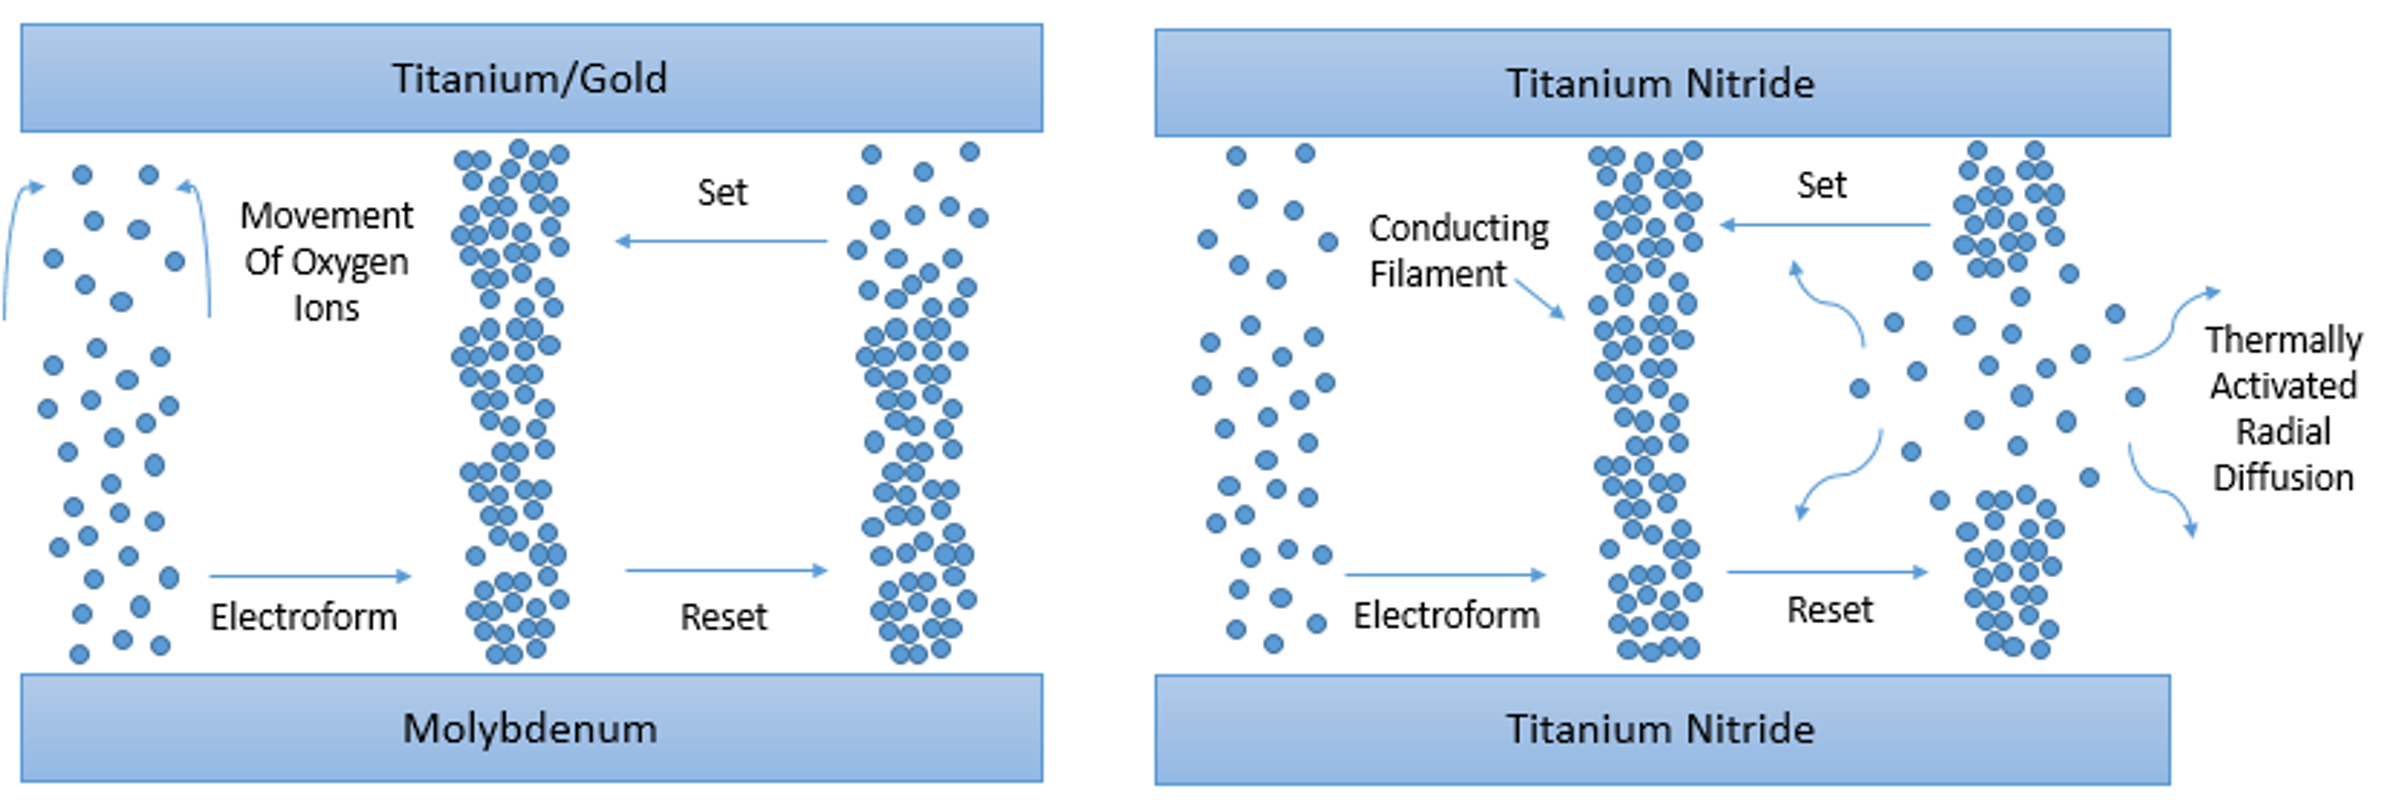
\includegraphics[width=0.95\textwidth]{Chapter3/Figs/v.png}
    \caption[Schematic of switching mechanism in SiOx devices.]{Schematic of bipolar switching in asymmetric devices (left) and of unipolar switching in symmetric devices (right).}
    \label{fig:3v}
\end{figure}

\noindent The phenomenon of bipolar switching in asymmetric devices can be described in qualitative terms as the movement of oxygen through a thin silicon oxide film (Figure \ref{fig:3v}). This phenomenon can be attributed to the deformation occurring in proximity to the electrode surface, which facilitates the injection of electrons and subsequent release of oxygen molecules. In the absence of any external damage, the silicon oxide of the device contains oxygen vacancies, i.e. structural defects. \\

\noindent The defects under scrutiny were formed during the fabrication process and were distributed evenly throughout the amorphous structure. It has been established that, under ambient temperature conditions, the diffusion of these defects occurs at a relatively slow rate. This is attributed to the presence of a substantial diffusion barrier. \\

\noindent When a voltage bias is applied to the material, these structural defects can rearrange into different configuration, while additional defects are also generated. The diffusion barrier in silicon oxide is significantly reduced with the new configuration. This enables negative oxygen ions to travel faster towards the positive electrode.\\

\noindent These oxygen anions are eventually trapped at the metal-oxide interface. The anions then discharge and form oxygen molecules $O_2$. Under extreme conditions, enough oxygen molecules built-up at the interface can cause bubbles of oxygen to form and eventually burst at the electrode surface, in the form of super oxide. \\

\noindent In operating conditions, the movement of oxygen ions within the oxide facilitates the electrical properties of the device. When an electric field below electric breakdown is applied to the device, the configuration changes can be conceptualised as the electroforming process for RRAM. The alterations in the distribution of oxygen vacancies are terminated once an abrupt conductance change has occurred, thereby forming a conductive filament in the silicon oxide film.\\

\noindent It is hypothesised that trap-assisted tunnelling is the predominant mode of carrier transport for bipolar switching. This finding indicates that the conductive filament within the material is not continuous, but rather consists of a series of neighbouring oxygen vacancies. The lower barrier heights observed in the preceding section indicate the occurrence of electron conduction through oxygen vacancy defects. Once the conductive filament has been formed under controlled breakdown conditions, the subsequent diffusion of oxygen vacancies is known to control the switching mechanism in bipolar mode, possibly via a local redox process occurring at the metal-oxide interface.\\

\noindent The process of bipolar switching is primarily governed by the movement of oxygen ions in response to an externally applied electric field. Conduction in unipolar switching mode is likely to share some similarity with bipolar switching. A significant distinction pertains to the reset process in these devices.\\

\noindent The conductive filament in unipolar switching samples can be conceptualised as exhibiting slightly greater continuity, thereby facilitating enhanced ohmic conduction. Consequently, a thermal effect is associated with the current passing through the filament during the switching process. The occurrence of a critical current threshold may result in the abrupt rupture of the conducting filament via thermally activated diffusion or Joule heating, thereby effecting a reset of the device.\\

\noindent In summary, it has been observed that resistive switching in metal oxides may be attributed to the presence of oxygen vacancies in the conductive filaments of silicon oxide. The role of the applied electric field is also of significance in the switching process, particularly in the context of bipolar switching, and in conjunction with Joule heating in the case of unipolar switching.\\

\noindent In the set process, oxygen anions are known to drift towards the electrode. This process results in the formation of positive oxygen vacancies, which facilitate the conduction of electrons. In the reset process, the oxygen ions residing near the metal-insulator interface are displaced into the vacancies. Alternatively, a sufficiently high local Joule heating can also overcome the vacancies binding energies. In either scenario, the conductive filament is ruptured and the device is reset.


\section[Summary]{Summary}

The primary insulating layer material for the devices and samples examined in this study is silicon dioxide ($SiO_x$) \cite{mehonic2012resistive}, in conjunction with electrode materials such as silver ($Ag$) or copper ($Cu$). Silicon-rich silica, which is predominantly utilised in the insulating layer, exhibits considerable promise for fully CMOS-compatible processing. A silicon oxide electron injection model has been developed to facilitate a more profound comprehension of the characteristics of silicon oxide \cite{gao2016mechanism}. \\

\noindent The amorphous silicon oxide structure exhibits $O-Si-O$ bonds, with a subset of these bonds featuring broad angle bonds, which possess the capacity to function as deep electron traps, with the capability to capture two electrons. The $Si-O$ bond is subsequently weakened once the broad bonds have collected both electrons. This reduction in energy requirement is attributed to the minimisation of the force required to break the connection and create the Frenkel defect. The formation of these defects gives rise to a population of vacancies, which can then contribute to the formation of the conductive filament. \\

\noindent Following an investigation into the underlying physics of the materials and mechanisms that comprise new RRAM devices, it is advantageous to analyse general device behaviours in terms of overall $I-V$ characteristics, volatility, polarity dependence, and power consumption, with a view to enhancing application design. This analysis would facilitate improved application design. RRAM devices have been shown to respond in three distinct ways \cite{li2017resistive}. \\

\noindent The classification of these as unipolar is predicated on the premise that they are set and reset with the same polarity. The term "bipolar" is employed to describe a device that has been successfully set and reset with opposing polarities. Finally, threshold switching occurs when a device transitions to its low resistance state within a certain voltage range. \\

\noindent Additionally, the term 'nonpolar' is employed to denote devices that are characterised by polarity independence, thereby enabling them to execute both unipolar and bipolar operations. As illustrated in Figure \ref{fig:3w}, these three groups can be summarised as follows. \\

\begin{figure}[htbp!] 
    \centering    
    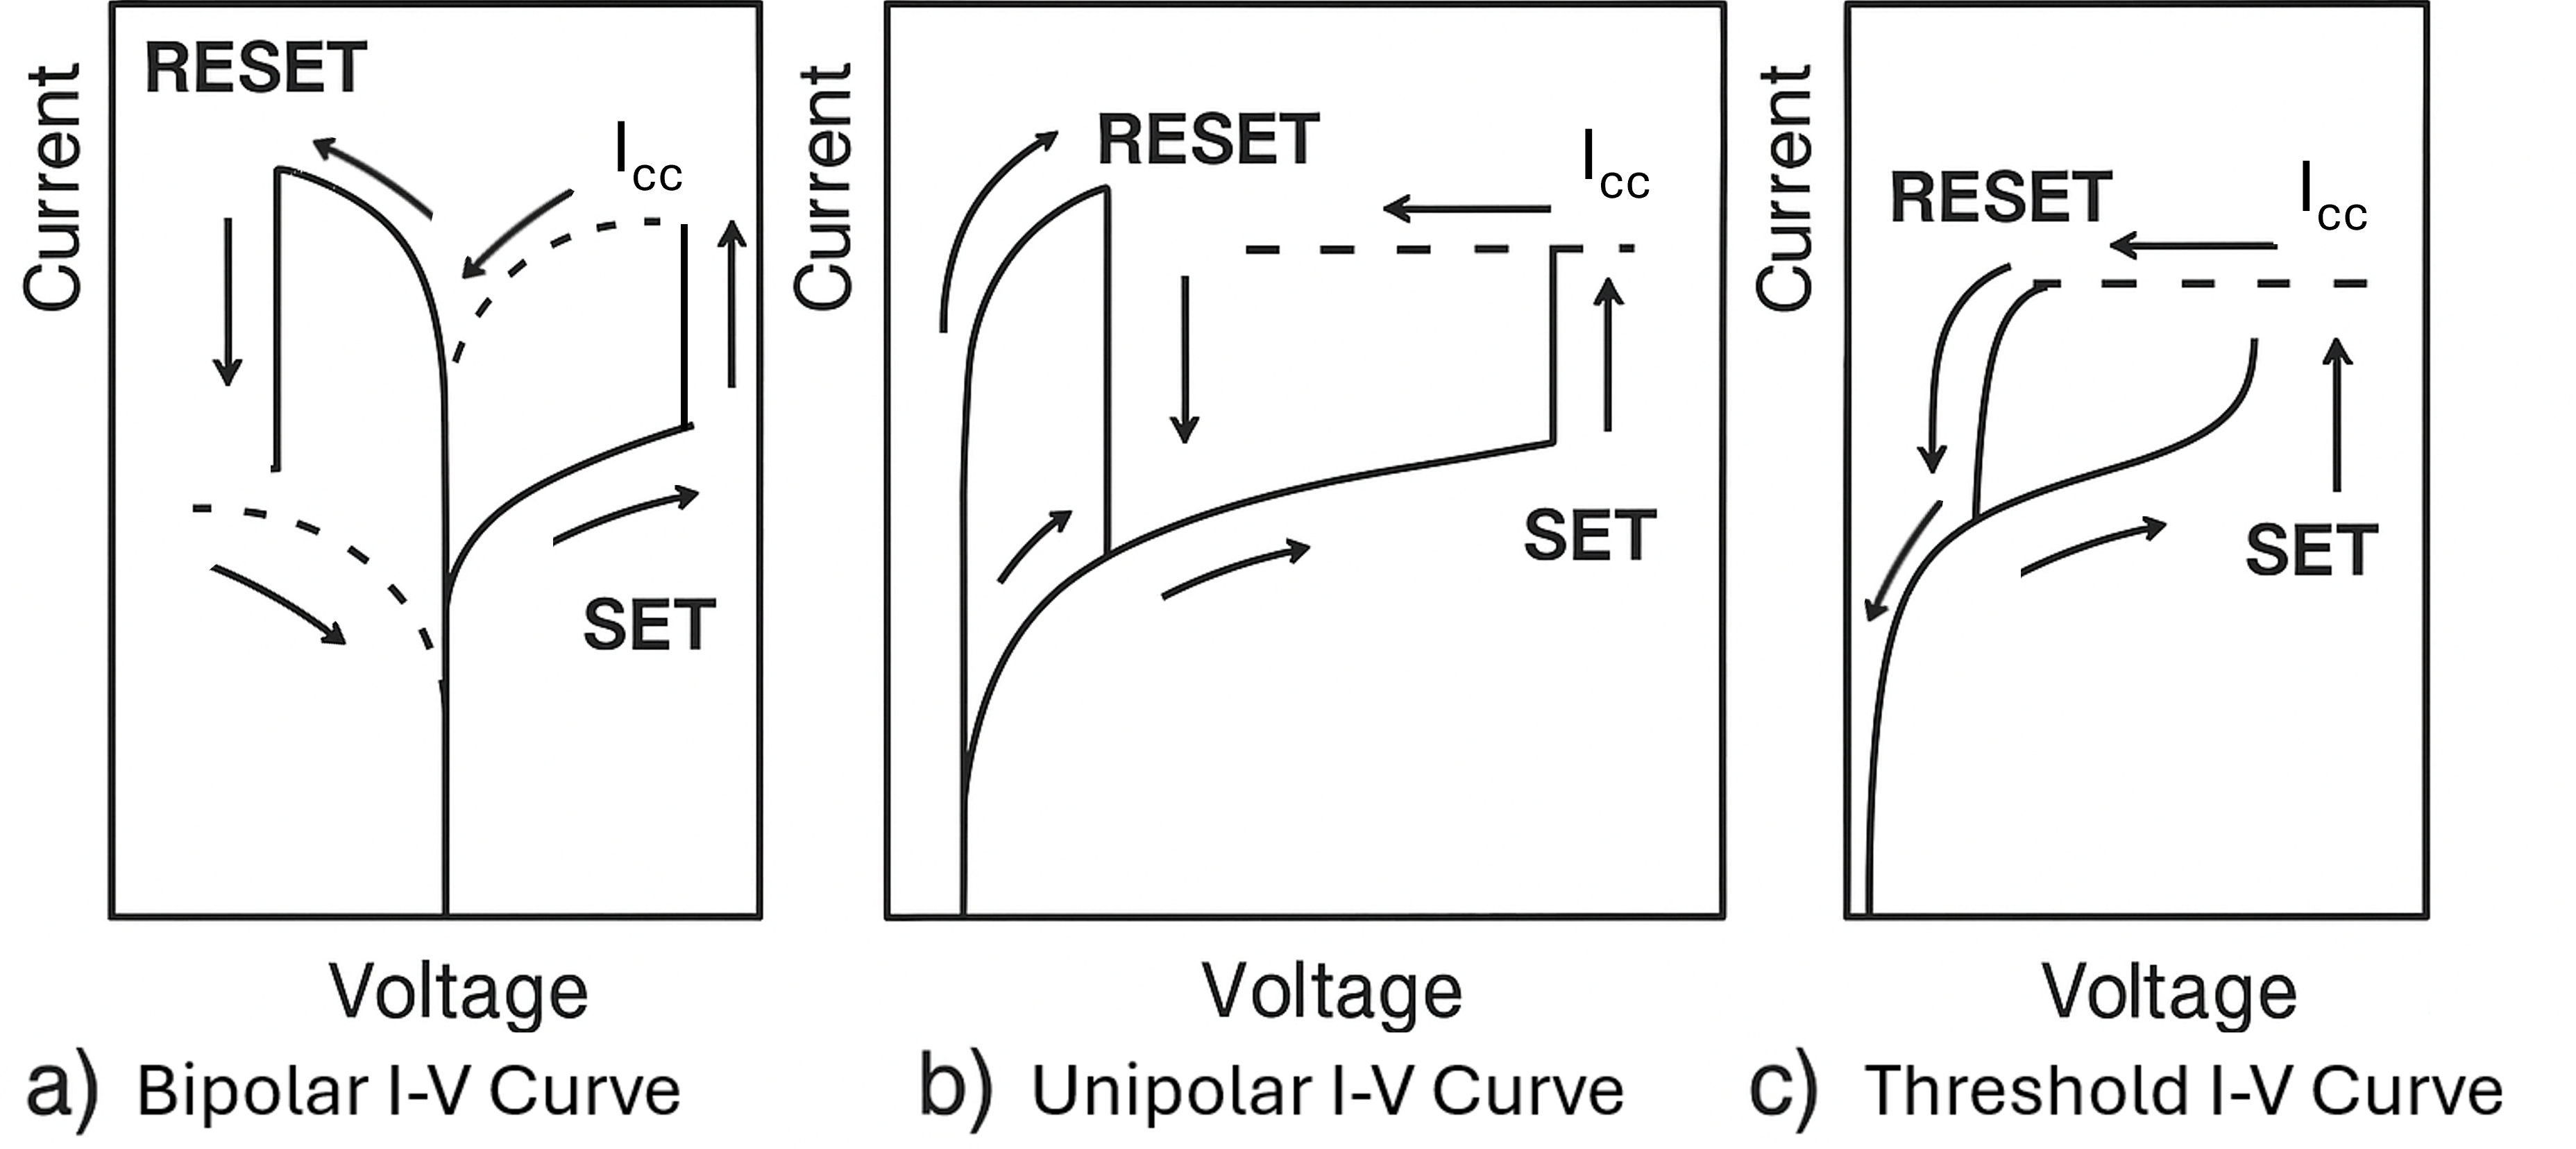
\includegraphics[width=1\textwidth]{Chapter3/Figs/w.png}
    \caption[Schematic I-V curves.]{Schematic I-V curves in: a) non-volatile bipolar memory switching mode, b) non-volatile unipolar memory switching mode; and c) volatile threshold switching mode. In the SET process, a compliance current is required to avoid hard breakdown \cite{li2017resistive}.}
    \label{fig:3w}
\end{figure}

\noindent Bipolar switching involves setting and resetting devices in opposing polarities. This behaviour has been observed in a variety of oxide materials \cite{wei2008highly}. The switching method requires current compliance during setup, but it can be reset with the same applied current compliance. \\

\noindent In comparison to the unipolar switching strategy, this results in a significantly simpler compliance system. The magnitude of the switching voltage for bipolar devices is generally within the limits for digital chip integration. For example, the operational voltages can be sub $\pm 1V$ in both polarities \cite{menke2009separation}. \\

\noindent Unipolar switching, like bipolar switching, has been demonstrated in a variety of oxide materials \cite{jeong2007coexistence}. Under unipolar operation, electroforming and setting are field-driven processes, whereas resetting is typically a current-driven one. To eliminate rivalry between the two working systems, a current compliance must be imposed during the set process, as resetting is triggered by excessive currents. Once the device has been set, the current compliance can be increased or removed completely to allow a sufficient amount of current to flow and the device to reset. \\

\noindent The capacity of the unipolar device to function with a single supply rail allows it to be combined with digital integrated circuits. A rather sophisticated current compliance system, on the other hand, remains one of the main downsides of such devices, with the high reset current causing heating and power consumption difficulties, particularly when scaling big memory arrays \cite{yun2007random}. \\

\noindent Threshold switching occurs when a device flips to a low resistance state when the applied voltage reaches a threshold and then instantly resets when the voltage falls below a lower threshold, demonstrating hysteresis. \cite{adler1980threshold}. This phenomenon was proposed as a result of heat dissipation after evaluating the varied thicknesses of the bottom electrode \cite{chang2008effects}. This implies that changing the size of the electrode during the fabrication process can result in different intended threshold switching behaviors. \\

\noindent Aside from the switching processes, several aspects must be addressed when developing RRAM. To start, OxRAM samples usually have a lower on/off conductance ratio in the range of 10s–100s and offer good retention of up to $10^{12}$ cycles\cite{ielmini2010resistance}, while the CBRAM on/off conductance ratio can be fairly high in the range of $10^3$–$10^6$, but has limited endurance to less than $10^4$ cycles \cite{ambrogio2014statistical1}. \\

\noindent The unpredictability of switching parameters resulting from the stochastic behaviour of oxygen or metal ions during ionic migration, as well as the variability in filament form from device to device and cycle to cycle within a single device, provide a significant difficulty for the design of RRAM cells \cite{ambrogio2014statistical2}. As a result of these variations, the density of RRAM prototypes ready for commercialization is quite low at $\sim 4 Mb$. \\

\noindent Recent research has made tremendous progress in demonstrating the potential of high-density devices with remarkable attributes and low power consumption of $\sim$0.1 pJ \cite{yang2013memristive}, better reliability with endurance of more than $>10^{12}$ cycles and retention of $>10$ years at $150^{\circ}C$ \cite{hu2014review}, higher density of 32 Gb via a simpler fabrication steps and stronger thermal characteristics \cite{cha2013nanoscale}. This, together with the significant resistance variation not just between different devices but also inside and between programming cycles on the same device \cite{moore2006lithography}, has resulted in concerns with the repeatability of their electrical properties. These issues, taken together, have prevented RRAM from being commercialised, despite its many appealing characteristics. \\

\noindent Fortunately, the main deep learning-based neural processing techniques—such as regression, pattern recognition, and speech recognition—are random in nature and need less precise computation than deterministic traditional computing. As a result, compared to memory applications, variation in memory devices during manufacture has less of an influence on computation outcomes \cite{malik2013governing}. The more tolerated necessity for variation in neural applications, combined with recent technical advancement, has contributed to generate additional possibilities for RRAM devices to become suitable candidates for neural technologies.
%!TEX root = ../thesis.tex
%*******************************************************************************
%****************************** Fourth Chapter **********************************
%*******************************************************************************
\chapter{Current Transients in Memristive Devices}


\section[The Subthreshold Regime]{The Subthreshold Regime}

The initial primary focus of this thesis is on the characterisation of silicon-based memristors, which are the fundamental components of memristive systems. Since the discovery of the memristor and its importance to replicating synaptic activity had such a profound impact on the field of neuromorphic engineering, investigating additional nanoelectronic components and behaviours in this context will lead to new neuromorphic computing applications. \\

\noindent This chapter investigates a phenomenon known as the "current transient" that has yet to be deliberately applied to the demand of neuromorphic computing. The current transient phenomenon can be similarly represented by the current flowing through a defective capacitor in response to a step potential to produce rich dynamics, both growing and decreasing in conductance, and can be beneficial in a computational device. \\

\noindent This chapter begins by documenting and characterising the current transients based on available literature. The experimental procedures used throughout the chapter were then described, and strategies were developed to aid in the characterisation of current transients. This provides a deeper understanding of the physical models underpinning the transients, allowing for the further development of an integrative memristive system based on silicon oxide samples that are already available.

\subsection[Foundational Properties]{Foundational Properties}

Fundamentally, the processes of capacitive decay and dielectric relaxation are ideal to define a capacitor's response to a step voltage. Applying a constant voltage across its terminals causes the device current to decline until it ultimately comes to rest at a constant leakage current. This, however, is not always the case. When the voltage is applied for an extended period of time or at a high enough temperature, the current flowing through the device begins to grow as the oxide gets faulty and its resistance falls. This is known as oxide deterioration, an umbrella word for an oxide coating that becomes faulty over time as a result of environmental stress factors \cite{ghibaudo1999emerging}. \\


%!TEX root = ../thesis.tex
%*******************************************************************************
%****************************** Fifth Chapter **********************************
%*******************************************************************************
\chapter{Neuromorphic Modelling Framework}

\section[Optically Active Device]{Optically Active Device}

% This chapter presents a model for resistance switching devices that demonstrates both analogue potentiation and conductance depression under the same voltage polarity, exploring the subthreshold regime with current transients, which has the potential to simplify neuromorphic circuits. The utilisation of an empirical SPICE model enables the simulation of these transients, with the process of validation achieved through the use of experimental data. \\

% \noindent This provides parameters for simulations and facilitates applications such as fault mobility estimation and neuromorphic circuit functions. The enhancements made to the previous model include the integration of diodes to emulate Schottky-like contact and the incorporation of relaxation dynamics upon the removal of step potentials or the grounding of the device.

This chapter introduces a comprehensive modelling framework for resistance switching devices that exhibit both analog potentiation and conductance depression under the same voltage polarity. The model specifically explores the subthreshold regime with current transients, offering a pathway to simplifying neuromorphic circuit designs. By developing an empirical SPICE model validated against experimental data, this work provides crucial parameters for simulations, facilitating applications such as fault mobility estimation and advanced neuromorphic circuit functions. \\

\noindent A key enhancement to previous models includes the integration of diodes to emulate Schottky-like contacts and the incorporation of relaxation dynamics upon the removal of step potentials or grounding of the device. This modeling effort directly supports the advancement of energy-efficient and biologically inspired neuromorphic hardware by providing a robust tool to understand and predict complex device behaviors essential for event-driven computing and synaptic emulation.

\subsection[Modified Device Stack]{Modified Device Stack}

% A distinct set of devices with disparate top electrical contacts were characterised, one with conductive indium tin oxide (ITO) in lieu of gold. The bottom contact and oxide layer remained unaltered and consistent with those observed in the gold-contacted devices presented in the preceding section. When subjected to stress, the ITO-contacted device exhibited a distinct response compared to the gold-titanium contacted device. Instead of a gradual and smooth increase in conductance, the response was more erratic and chaotic. \\

% \noindent The aluminium-contacted devices have yet to demonstrate the occurrence of current transients following the application of stress. In addition to failing to exhibit current transients, any increase in conductance induced by the constant current stress is also observed to be more volatile than that observed in the other devices, with the devices returning to a high resistance state within a couple of hours.\\

The characterization of a distinct set of devices featuring disparate top electrical contacts, specifically conductive indium tin oxide (ITO) instead of gold, revealed unique stress responses. The bottom contact and silicon oxide (SiOx) layer remained consistent with those previously observed in gold-contacted devices. When subjected to electrical stress, the ITO-contacted device exhibited a response markedly different from the gold-titanium contacted device. Instead of a gradual and smooth increase in conductance, a more erratic and chaotic response was observed. Aluminium-contacted devices, in contrast, consistently failed to demonstrate current transients following the application of stress. Any increase in conductance induced by constant current stress in these devices also proved more volatile, with the devices returning to a high resistance state within a couple of hours.\\

\begin{table}[ht]
    \caption{Comparison of the modified device stacks.}
    \centering
    \begin{tabular}{|cc|cc|}
    \hline
    \multicolumn{2}{|c|}{Original Stack}              & \multicolumn{2}{c|}{Modified Stack}              \\ \hline
    \multicolumn{1}{|c|}{Layer} & Film Thickness (nm) & \multicolumn{1}{c|}{Layer} & Film Thickness (nm) \\ \hline
    \multicolumn{1}{|c|}{Au}    & 110                 & \multicolumn{1}{c|}{ITO}   & 30                  \\ \hline
    \multicolumn{1}{|c|}{Ti}    & 3                   & \multicolumn{1}{c|}{Ti}    & 3                   \\ \hline
    \multicolumn{1}{|c|}{SiOx}  & 35                  & \multicolumn{1}{c|}{SiOx}  & 20                  \\ \hline
    \multicolumn{1}{|c|}{Mo}    & 280                 & \multicolumn{1}{c|}{Mo}    & 150                 \\ \hline
    \end{tabular}
    \label{table:5a}
\end{table}


% \noindent In contrast, the ITO contacted devices did exhibit transients, but interestingly, only partially. A typical transient observed in ITO devices is plotted in Figure \ref{fig:5a}. It exhibits the initial increase in conductance as is typical with current transients, but does not then start reducing in conductance. Instead, the device exhibits a chaotic spiking-like behaviour which, if observed for too long, will cause the device to switch to a low resistance state.\\

\noindent The ITO-contacted devices, however, did exhibit partial current transients. A typical transient observed in these devices, as plotted in Figure \ref{fig:5a}, showed an initial increase in conductance, characteristic of current transients. However, it notably did not then commence a reduction in conductance; instead, the device displayed chaotic spiking-like behavior. Prolonged observation of this behavior would typically lead to the device switching to a low resistance state.\\

\begin{figure}[htbp!] 
    \centering    
    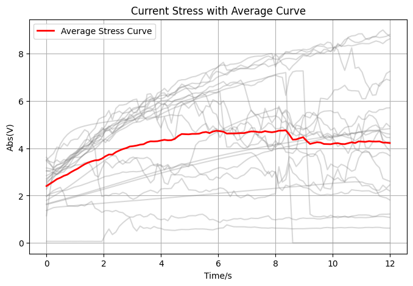
\includegraphics[width=0.6\textwidth]{Chapter5/Figs/a.png}
    \caption[Stressing responses of ITO top contacted device.]{Stressing responses of ITO top contacted device. With the objective to ascertain the stress responses of the ITO top-contacted device, the voltage across the device was monitored while it was subjected to a constant current of $-0.5\mu A$. It was not possible to apply larger currents. The response was observed to be less smooth when compared to that of the gold-contacted device.}
    \label{fig:5a}
    \end{figure}

% \noindent The observation of a partial current transient in ITO-contacted devices is a significant finding. As will be discussed in the following section, this evidence is indicative of the transient being the result of multiple simultaneous changes occurring in the device. Furthermore, it supports the hypothesis that the top metal-insulator interface plays a role in generating transients.\\

% \noindent The hypothesis that alterations to specific interfaces of the device can influence the characteristics of the current transient is supported by findings in tantalum oxide-based devices \cite{tuller2011point}. In this study, a layer of $Al_2O_3$ was deposited between the tantalum oxide bulk and the titanium nitride electrodes, which reduced the prominence of the current transient in the absence of the buffer layer.\\

\noindent The observation of a partial current transient in ITO-contacted devices is a significant finding, as it indicates the transient results from multiple simultaneous changes within the device. This evidence supports the hypothesis that the top metal-insulator interface plays a crucial role in generating these transients. The notion that alterations to specific interfaces can influence the characteristics of the current transient is further supported by findings in tantalum oxide-based devices, where a layer of$Al_2O_3$ deposited between the tantalum oxide bulk and titanium nitride electrodes reduced the prominence of the current transient in the absence of the buffer layer \cite{tuller2011point}.\\

% \noindent To illustrate, the gradual decline in conductance of the transients is exclusive to the gold-contacted device, indicating that it is either due to the characteristics of the metal-insulator interface or the disparate responses to stressing at this interface that determine whether the decaying behaviour is manifested. \\

% \noindent In contrast, the initial increase in conduction is observed in both the ITO and gold-contacted devices. This suggests that the behaviour is less affected by the top metal-insulator interface and may be located in the bulk oxide layer or at the bottom metal-insulator interface. The disappearance of the slower decay in conductance with the change in top electrode may provide insight into the physical model describing the current change. 

\noindent Specifically, the gradual decline in conductance of the transients is exclusive to the gold-contacted devices, suggesting that it is either due to the characteristics of the metal-insulator interface or the disparate responses to stressing at this interface that determine whether the decaying behavior is manifested. Conversely, the initial increase in conduction is observed in both ITO and gold-contacted devices, implying that this behavior is less affected by the top metal-insulator interface and may instead be attributed to changes within the bulk oxide layer or at the bottom metal-insulator interface. The disappearance of the slower conductance decay with the change in top electrode thus provides valuable insight into the physical model describing the current change, reinforcing the idea of distinct underlying mechanisms.

\subsection[Conductance Variation Mechanisms]{Conductance Variation Mechanisms}

% The initial step is to ascertain the location within the device stack where alterations are taking place that are responsible for the observed reduction in conductance. The absence of decay occurring concurrently with the alteration of the top electrode suggests that the causal factor responsible for the observed conductance decay is situated at the interface between the top electrode and the amorphous silicon dioxide. \\

\noindent Ascertaining the precise location within the device stack responsible for the observed reduction in conductance is the initial step in understanding these mechanisms. The absence of decay concurrently with the alteration of the top electrode strongly suggests that the causal factor for the conductance decay is situated at the interface between the top electrode and the amorphous silicon dioxide. Given the slow dynamics of this change, a drift of some mobile defect is plausibly responsible.\\

% \noindent Given the slow dynamics of the change in conductance, it is plausible that a drift of some mobile defect is responsible. It is well established that silicon dioxide films are susceptible to the influence of alkali mobile ions \cite{snow1965ion}, including sodium and lithium ions, which are all characterised by a positive charge \cite{yon1966sodium}. The drift of these mobile charges can significantly affect the potential drops at metal-oxide interfaces, as well as modulate barrier heights when allowed to accumulate.\\

% \noindent If some positive mobile ion, regardless of the species, existed in the oxide of the device, it would be attracted to the top electrode, which is at a negative potential. This would cause an accumulation of positive space charge at the interface, which would in turn reduce the potential across the oxide. Nevertheless, it can be argued that alkali metals, such as sodium and potassium, are unlikely to be the cause of this positive space charge, given that they do not migrate at room temperature. \\

% \noindent Instead, they require temperatures in excess of 100 degrees Celsius (212 degrees Fahrenheit) \cite{deal1974current}. The current transients presented in this thesis are all observed at room temperature, which suggests the need for an alternative candidate to explain the mobile space charge, in particular one that is mobile at room temperature. \\

\noindent Silicon dioxide films are well-established as susceptible to the influence of alkali mobile ions, such as positively charged sodium and lithium ions \cite{snow1965ion, yon1966sodium}. The drift of these mobile charges can significantly affect potential drops at metal-oxide interfaces and modulate barrier heights upon accumulation. Nevertheless, it is unlikely that alkali metals are the sole cause of this positive space charge, as their migration typically requires temperatures exceeding $100^\circ C$ \cite{deal1974current}. All current transients presented in this work were observed at room temperature, necessitating an alternative candidate for the mobile space charge—one that is mobile under ambient conditions.\\

% \noindent It is noteworthy that modelling of the temperature within analogous $TaO_x$ devices has indicated the potential for increases in oxide temperature of up to 100°C with applied voltages of -0.7 to -1.8V due to Joule heating \cite{shen2021experimentally}. This would imply that if comparable effects were present during the current transient, then elevated temperatures within the oxide could be occurring and potentially facilitating the migration of alkali metal defects.\\

\noindent It is worth noting that modelling of the temperature within analogous $TaO_x$  devices has indicated the potential for increases in oxide temperature of up to  $100^\circ C$ with applied voltages of -0.7V to -1.8V due to Joule heating \cite{shen2021experimentally}. If comparable effects were present during the current transient, then elevated temperatures within the oxide could potentially facilitate the migration of alkali metal defects.\\

% \noindent It seems plausible to suggest that the proton \cite{hofstein1967proton} is a likely candidate for positive ions that are mobile at room temperature. The presence of ionised hydrogen in silicon dioxide films has been repeatedly observed to be both stable and consistent \cite{vanheusden1998chemical}. It has been demonstrated that protons can influence the electronic properties of capacitor devices in which protons are trapped within the oxide \cite{vanheusden1999non}. Their long-term stability has been demonstrated through multiple cycles of migration between device electrodes \cite{warren1997protonic}. \\

% \noindent It is commonly assumed that these ions are introduced during the growth of the oxide \cite{vanheusden1998thermally}. Furthermore, their concentration has been demonstrated to increase through annealing in an atmosphere at temperatures above 200 degrees Celsius \cite{lifshitz1989detection}. However, their presence has also been introduced electronically via the electrolysis of water within the device and via radiation \cite{winokur1977field}. It is also noteworthy that their migration has been shown to occur repeatedly at room temperature.\\

\noindent The proton \cite{hofstein1967proton} emerges as a more likely candidate for positive ions mobile at room temperature. Ionized hydrogen in silicon dioxide films has been repeatedly observed to be both stable and consistent \cite{vanheusden1998chemical}. Protons have been demonstrated to influence the electronic properties of capacitor devices where they are trapped within the oxide \cite{vanheusden1999non}, and their long-term stability has been shown through multiple cycles of migration between device electrodes \cite{warren1997protonic}. These ions are commonly assumed to be introduced during oxide growth \cite{vanheusden1998thermally}, with their concentration increasing through annealing in an atmosphere at temperatures above $200^\circ C$ \cite{lifshitz1989detection}. Their presence can also be introduced electronically via the electrolysis of water within the device and through radiation \cite{winokur1977field}. Crucially, their migration has been shown to occur repeatedly at room temperature.\\

% \noindent This raises the question of why the accumulation of protons occurs exclusively in the gold-contacted devices, rather than in the ITO. Given that gold is an inert metal and is unlikely to be reduced by protons, the accumulation at the gold interface is to be expected. In contrast, there is a substantial body of evidence indicating that the ITO would be reduced in the presence of protons.\\

% \noindent Although ITO contacts are often considered to be inert in certain electrochemistry scenarios, this is not always the case. Their reduction is, in fact, heavily dependent on the pH of the electrolyte. For instance, the reduction of the electrode has been observed on numerous occasions in acidic electrolytes \cite{ciocci2021differentiating,senthilkumar2008electrochemical}. \\

\noindent The question then arises as to why the accumulation of protons occurs exclusively in gold-contacted devices, but not in ITO. Given that gold is an inert metal and is unlikely to be reduced by protons, their accumulation at the gold interface is expected. In contrast, substantial evidence indicates that ITO would be reduced in the presence of protons. Although ITO contacts are often considered inert in certain electrochemistry scenarios, their reduction is, in fact, heavily dependent on the pH of the electrolyte. For instance, electrode reduction has been observed numerous times in acidic electrolytes \cite{ciocci2021differentiating, senthilkumar2008electrochemical}.\\

% \noindent The reduction of ITO in the presence of acids has been demonstrated in both electrochemical experiments conducted at room temperature \cite{wang2003optical} and in instances where ITO has been exposed to a hydrogen plasma \cite{banerjee1987degradation}. In one study, the application of negative voltages to an ITO electrode immersed in hydrochloric acid resulted in the formation of spherical structures at the grain boundaries of the ITO film, which exhibited a metallic-like appearance [88]. \\

% \noindent Following characterisation with Energy dispersive x-ray Spectroscopy (EDS) \cite{huang2003electrochemical} and X-ray Diffraction (XRD) in a separate study \cite{liu2015important}, the spherical regions were found to be depleted of oxygen or exhibited only peaks of indium and tin, providing compelling evidence that these spheres were metallic. The same spherical structures were observed in ITO films exposed to a hydrogen plasma, which, when analysed with Auger spectroscopy, again revealed a lower oxygen concentration in the spherical regions.\\

\noindent The reduction of ITO by protons has been demonstrated in both electrochemical experiments at room temperature \cite{wang2003optical} and in instances where ITO has been exposed to a hydrogen plasma \cite{banerjee1987degradation}. One study found that applying negative voltages to an ITO electrode immersed in hydrochloric acid led to the formation of metallic-appearing spherical structures at the grain boundaries of the ITO film \cite{huang2003electrochemical}. Characterization with Energy Dispersive X-ray Spectroscopy (EDS) \cite{huang2003electrochemical} and X-ray Diffraction (XRD) \cite{liu2015important} revealed these spherical regions were depleted of oxygen or exhibited only peaks of indium and tin, providing compelling evidence of their metallic nature. Similar spherical structures were observed in ITO films exposed to a hydrogen plasma, with Auger spectroscopy again showing lower oxygen concentrations in these regions.\\

% \noindent The reduction of ITO by protons may provide an explanation for the absence of space charge accumulation in ITO-contacted devices. Instead of accumulating, the protons reduce the ITO, producing water as a byproduct, which would not contribute to a positive space charge. Furthermore, the reduction of the electrode may also elucidate the more erratic current-time response observed in ITO devices, as the electrode structure undergoes substantial alterations.\\

\noindent The reduction of ITO by protons may provide a compelling explanation for the absence of space charge accumulation in ITO-contacted devices. Instead of accumulating, the protons reduce the ITO, producing water as a byproduct, which would not contribute to a positive space charge. Furthermore, the reduction of the electrode may also elucidate the more erratic current-time response observed in ITO devices, as the electrode structure undergoes substantial alterations.\\

% \noindent The potential for structural changes to occur in both the oxide and the metal contacts makes it challenging to determine the specific role each plays in modulating the device's conductance. In order to investigate the effect of the contact, it would be beneficial to fabricate and characterise devices with a variety of contact materials. \\

% \noindent Any discrepancies in the observed behaviour between the devices could be ascribed to the metal or the metal-insulator interface, whereas any enduring effects could be attributed to the oxide. To further examine any behaviour attributed to the oxide, devices of varying oxide thicknesses could be fabricated. This may reveal a dependence on the oxide thickness, which could be supporting evidence for the oxide having a role in the changing device conductance. \\

% \noindent However, it is important to exercise caution when drawing conclusions from this approach, as the change in oxide thickness will also modify the magnitude of the current density flowing through the device, potentially affecting the interfaces. The fabrication of devices with different oxide thicknesses and a variety of metal contacts is a future research direction. \\

\noindent The potential for structural changes to occur in both the oxide and the metal contacts makes it challenging to definitively determine the specific role each plays in modulating the device's conductance. To investigate the effect of the contact, it would be beneficial to fabricate and characterize devices with a variety of contact materials. Any discrepancies in observed behavior between these devices could be ascribed to the metal or the metal-insulator interface, while any enduring effects could be attributed to the oxide. To further examine any behavior attributed to the oxide, devices of varying oxide thicknesses could be fabricated. This might reveal a dependence on oxide thickness, offering supporting evidence for the oxide's role in changing device conductance. However, caution must be exercised, as changes in oxide thickness also modify the magnitude of the current density flowing through the device, potentially affecting the interfaces. The fabrication of devices with different oxide thicknesses and a variety of metal contacts remains a promising future research direction.\\

% \noindent If the hypothesis that the transient is the result of two separate changes is true, then it would suggest that devices could potentially be made to exhibit only one of these changes in isolation. Fabrication of such a device would provide strong supporting evidence for the hypothesis and a clear demonstration that the changes are separable. Modification of the top contact material appears to facilitate this separation.\\



% \noindent Devices fabricated with a conductive ITO top electrode, in lieu of the gold-titanium contact, do not exhibit the anticipated decay in conductance; rather, they display only the initial increase. Figure \ref{fig:3h} illustrates the current-time response of an ITO-contacted device. As observed previously in the gold devices, the current begins to increase; however, it never reaches the inflection point. Instead, it continues to increase in conductance, becoming progressively noisier until the device undergoes breakdown.\\

\noindent If the hypothesis that the transient is the result of two separate changes is valid, it suggests that devices could potentially be engineered to exhibit only one of these changes in isolation. Fabricating such a device would provide strong supporting evidence for the hypothesis and a clear demonstration of the separability of these mechanisms. Modification of the top contact material, as observed with ITO, appears to facilitate this separation. Devices fabricated with a conductive ITO top electrode, in lieu of the gold-titanium contact, display the initial increase followed by instabilities. Figure \ref{fig:5b} illustrates the current-time response of an ITO-contacted device. As observed previously in gold devices, the current begins to increase; becoming progressively noisier until the device undergoes breakdown.\\

\begin{figure}[htbp!] 
    \centering    
    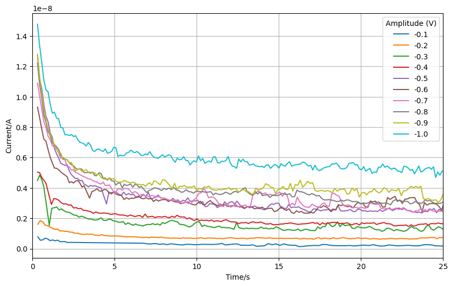
\includegraphics[width=0.6\textwidth]{Chapter5/Figs/b.png}
    \caption[The current-time response for a device with a conductive ITO top electrode.]{The current-time response for a device with a conductive ITO top electrode. The current is generated in response to a step potential applied to the top contact with respect to the bottom. It exhibits only the increase in conductance and not the decrease. As the current increases, the noise level also rises until the device reaches a point of breakdown. The structure of the device is identical to that of the gold-contacted devices, with the exception of the change in the top electrode's material from gold-titanium to indium tin oxide (ITO).}
    \label{fig:5b}
\end{figure}

% \noindent The ITO device has undergone a comparable stressing process to that of the gold devices, which is outlined in the preceding chapter. In the initial stages, the devices exhibit only capacitive currents and possess a very high resistance. Subsequently, a constant current stressing procedure is employed to produce a more conductive device. \\

% \noindent Following a period of relaxation, a repeatable transient is produced, provided that the applied voltage is maintained for a sufficiently brief duration to prevent breakdown of the device. A comparable phenomenon has been documented \cite{moon2019rram} in a variety of oxides and is frequently employed in the replication of short-term potentiation of synapses \cite{zhang2017emulating, chang2011short}.\\

% \noindent Furthermore, this absence of slower dynamics may corroborate with previous findings \cite{meyer2005oxygen}, where the slower dynamics were postulated to be attributable to oxygen vacancies. It is conceivable that the ITO contact is more prone to exchange oxygen with the oxygen vacancy than the inert gold contact. \\

\noindent The ITO device underwent a comparable stressing process to that of the gold devices. Initially, the devices exhibit only capacitive currents and possess a very high resistance. Subsequently, a constant current stressing procedure is employed to produce a more conductive device. Following a period of relaxation, a repeatable transient is produced, provided that the applied voltage is maintained for a sufficiently brief duration to prevent device breakdown. A comparable phenomenon has been documented in a variety of oxides \cite{moon2019rram} and is frequently employed in the replication of short-term potentiation of synapses \cite{zhang2017emulating, chang2011short}. Furthermore, this slower dynamic may corroborate previous findings \cite{meyer2005oxygen}, where slower dynamics were postulated to be attributable to oxygen vacancies. It is conceivable that the ITO contact is more prone to exchange oxygen with the oxygen vacancy than the inert gold contact.\\

\begin{figure}[htbp!] 
    \centering    
    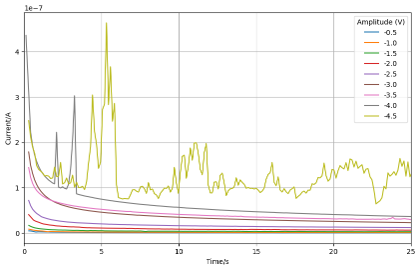
\includegraphics[width=0.6\textwidth]{Chapter5/Figs/c.png}
    \caption[instabilities of potentiation and depression on the amplitude of applied voltage pulses.]{instabilities of potentiation and depression on the amplitude of higher applied voltage pulses on ITO devices.}
    \label{fig:5c}
\end{figure}

% \noindent An alternative hypothesis is that the Au contact is diffusing through the oxide, whereas the ITO contact is not. Previous observations have shown that Au can form conductive bridges between two contacts through a thin film of $ZnO$ \cite{peng2012resistive}. Given that gold is known to diffuse in silicon dioxide films, this could be a possibility \cite{madams1974migration}. However, TEM analyses of the devices studied in this thesis have not produced observable gold filaments, casting doubt on this hypothesis \cite{mehonic2017intrinsic}.\\

\noindent An alternative hypothesis is that the Au contact is diffusing through the oxide, whereas the ITO contact is not. Previous observations have shown that Au can form conductive bridges between two contacts through a thin film of ZnO \cite{peng2012resistive}. Given that gold is known to diffuse in silicon dioxide films \cite{madams1974migration}, this could be a possibility. However, Transmission Electron Microscopy (TEM) analyses of the devices studied in this thesis have not produced observable gold filaments, casting doubt on this hypothesis \cite{mehonic2017intrinsic}.\\


% \noindent An additional potential explanation for the observed discrepancy in behaviour between the Au and ITO contacts is the possibility of differences in their respective work functions. While not directly measured on the samples in question, the work function of gold is reported to be between 4.9 and 5.2 electronvolts (eV) \cite{tran2019anisotropic}, while thin films of indium tin oxide (ITO) have been measured to have a work function between 4.25 and 4.28 eV \cite{schlaf2001work}. \\

% \noindent This could result in a difference in work function of approximately 1 eV. Such differences would lead to offsets in the band alignments at the contact and oxide, which could affect which traps within the oxide the electrons are injected into. As discussed in the previous chapter, the disappearance of the slower decay in conductance with the change in top electrode is suggestive of proton migration playing a role in the slower decay in device current.

\noindent An additional potential explanation for the observed discrepancy in behavior between the Au and ITO contacts is the possibility of differences in their respective work functions. While not directly measured on the samples in question, the work function of gold is reported to be between 4.9 and 5.2 electronvolts (eV) \cite{tran2019anisotropic}, whereas thin films of indium tin oxide (ITO) have been measured to have a work function between 4.25 and 4.28 eV \cite{schlaf2001work}. This could result in a work function difference of approximately 1 eV. Such differences would lead to offsets in the band alignments at the contact and oxide, which could affect which traps within the oxide the electrons are injected into. As discussed, the change in conductance dynamic with the alteration in top electrode is highly suggestive of proton migration playing a role in the slower decay in device current.

\section[Empirical Model Fitting]{Empirical Model Fitting}

% This section presents the development of empirical models designed to track the rates of increase and decrease in conductance separately. The models are primarily intended to quantify the rate of change in conductance. The question of a physical model will be addressed in the following section.

This section presents the development of empirical models designed to track the rates of increase and decrease in conductance separately. These models are primarily intended to quantify the rate of change in conductance, with the question of a comprehensive physical model addressed in subsequent discussions.

\subsection[Fitting Metrics]{Fitting Metrics}

% \noindent The models explored here are derived from the relaxation experiments that were previously outlined in the preceding chapter. It was evident that the gradual decline in device current delineated the upper limit of the maximum device current, while the initial surge in current approached this maximum but did not exceed it. 


% \noindent This is represented by the product of two time-dependent functions, $f_{inc}(t)$ and $f_{dec}(t)$. The increase in current is analogous to a charging term, $f_{inc}(t)$, which rises from 0 to 1. Initially, this function defines the device current. However, as $f_{inc}(t)$ approaches 1, it then allows the function it is multiplied with to define the total current, in this case  $f_{dec}(t)$. \\

\noindent The models explored here are derived from relaxation experiments previously outlined. It was evident that the gradual decline in device current delineated the upper limit of the maximum device current, while the initial surge in current approached this maximum but did not exceed it. This behavior is represented by the product of two time-dependent functions, $f_{inc}(t)$ and $f_{dec}(t)$. The increase in current is analogous to a charging term, $f_{inc}(t)$, which rises from 0 to 1. Initially, this function primarily defines the device current. However, as  $f_{inc}(t)$ approaches 1, it then allows the function it is multiplied with, $f_{dec}(t)$, to define the total current:
\begin{align}
    I(t) = f_{inc}(t) \times f_{dec}(t) \quad \forall \left\{ f_{inc}(t) \in [0 \to 1] : f_{dec}(t) \in \mathbb{R} \right\} \label{eq:5.1}
\end{align}

% \noindent Although this equation forms the basis of the empirical model, questions remain regarding the specific forms that $f_{inc}(t)$ and $f_{dec}(t)$ should take and the most appropriate means of comparing their effectiveness. The efficacy of each fitting equation is evaluated based on two criteria: the quality of the fit and the degree of realism of the fitted parameters in relation to the underlying physical system from which the model is derived.\\

% \noindent The correspondence between each term of a given model and a physical property is contingent upon the physical system from which the model is derived. These properties are assigned a range of values that are deemed realistic. Values outside of this range may indicate that the assumed model is not applicable. The specific correspondence between physical properties and terms is model-specific and will be detailed later in conjunction with the model.\\

\noindent While this equation forms the basis of the empirical model, the specific forms that $f_{inc}(t)$ and $f_{dec}(t)$ should take, and the most appropriate means of comparing their effectiveness, remain key considerations. The efficacy of each fitting equation is evaluated based on two criteria: the quality of the fit and the degree of realism of the fitted parameters in relation to the underlying physical system from which the model is derived. The correspondence between each term of a given model and a physical property is contingent upon the physical system from which the model is derived. These properties are assigned a range of values deemed realistic, with values outside this range potentially indicating that the assumed model is not applicable. The specific correspondence between physical properties and terms is model-specific and will be detailed later in conjunction with the model. \\

% \noindent The discrepancy between the fitted equation and the original experimental data is referred to as the residual. This can often be a useful visual indicator of the quality of the fit. An optimal fit would manifest residuals that are centered around zero, exhibiting no systematic offsets or time-variant components. \\

% \noindent The residuals in this form indicate that the fitted equation tracks the experimental data well, with the variances in the residuals around zero assumed to be a form of noise or variance in the original data. In contrast, a less optimal fit would exhibit systematic offsets that vary over time. This indicates that either an additional term is absent or the incorrect function has been selected. \\

\noindent The discrepancy between the fitted equation and the original experimental data is referred to as the residual. This can often serve as a useful visual indicator of the quality of the fit. An optimal fit would manifest residuals centered around zero, exhibiting no systematic offsets or time-variant components. Residuals in this form indicate that the fitted equation tracks the experimental data well, with variances around zero assumed to be a form of noise or variance in the original data. In contrast, a less optimal fit would exhibit systematic offsets that vary over time, indicating either an additional term is absent or an incorrect function has been selected.\\

% \noindent However, while residuals are useful for visually assessing a fit, they are less so when larger datasets are being fitted. Therefore, only one residual for each model is assessed, which is representative of the model's performance. The same experimental data will be fitted for each model, thus ensuring an accurate comparison. In order to assess a model's goodness of fit across a whole dataset, a single numerical metric that can quantify the fit is preferred.\\

\noindent While residuals are useful for visually assessing a fit, they are less so when larger datasets are being fitted. Therefore, only one residual for each model is assessed, chosen to be representative of the model's performance. The same experimental data will be fitted for each model, ensuring an accurate comparison. To assess a model's goodness of fit across an entire dataset, a single numerical metric that can quantify the fit is preferred.\\

% \noindent A more quantitative description of the goodness of fit is provided by the $R^2$ measure. The $R^2$ measure is a statistical tool that enables the comparison of the variance between the observed data points and the model's predicted values against the variance of the observed data and the mean of that data. In other words, it can be acknowledged that the most straightforward model for predicting a dataset would be to assume the mean value of the dataset in all cases.

\noindent A more quantitative description of the goodness of fit is provided by the $R^2$  measure. The $R^2$  measure is a statistical tool that enables the comparison of the variance between observed data points and the model's predicted values against the variance of the observed data and the mean of that data. In other words, the most straightforward model for predicting a dataset would be to assume the mean value of the dataset in all cases.\\
\begin{align}
SS_{tot} &= \sum_{i}\left( y_i - \bar y \right)^2 \label{eq:5.2} 
\end{align}

% \noindent In this case, the variance is defined by (\ref{eq:5.2}), Where $y_i$ is an individual datapoint and $\bar y$ is the mean average of the dataset, which is equal to the variance of the dataset. The variance of the dataset against the model's predictions can also be calculated with (\ref{eq:5.3}), Where $f_i$ is model’s predicted value at $i^th$ index, for any other model developed. \\

\noindent In this context, $SS_{tot}$ (Equation \ref{eq:5.2}) represents the total sum of squares, where $y_i$ is an individual data point and $\bar y$  is the mean average of the dataset, which is equal to the variance of the dataset. The variance of the dataset against the model's predictions, $SS_{res}$ , can be calculated using Equation (\ref{eq:5.3}), where $f_i$  is the model's predicted value at the $i^th$ index.
\begin{align}
    SS_{res} &= \sum_{i}\left( y_i - f_i \right)^2 \label{eq:5.3} 
\end{align}

% \noindent If the variance is similar to that of the dataset, the model is no more than a simple mean value predictor, and thus the data fit is poor. An alternative indication of a good fit is provided by a model with a variance much less than that of the dataset. However, residuals should still be checked. The $R^2$ value shown in (\ref{eq:5.4}), defined by the ratio of the variance of the model to the variance of the dataset, is based on this premise and increases as the model's fit improves.\\

\noindent If the model's variance is similar to that of the dataset, the model is no more than a simple mean value predictor, indicating a poor data fit. Conversely, a model with a variance much less than that of the dataset suggests a good fit, although residuals should still be checked. The $R^2$ value, defined by the ratio of the model's variance to the dataset's variance, is based on this premise and increases as the model's fit improves (Equation \ref{eq:5.4}).
\begin{align}
    R^2 &= 1 - \frac{SS_{res}}{SS_{tot}} \label{eq:5.4} 
\end{align}

% \noindent Notwithstanding the possibility of attaining an optimal fit, the values of the fitted parameters remain uncertain. To illustrate, a minimum in the fitting error could be achieved by a range of parameter values. This range is referred to as the confidence bounds, which can be interpreted as the range within which the fitting algorithm is certain the final value lies. \\

% \noindent For example, 90\% confidence bounds will define a range within which the algorithm is 90\% sure the optimal value can be found. If a higher confidence is required, the range will generally increase. Consequently, there is a trade-off between certainty and specificity. In this work, the standard confidence threshold of 90\% was employed.\\

% \noindent The choice of model for a particular dataset is influenced by the magnitude of the confidence intervals. If a model results in fitted parameters with large confidence intervals, it can present a challenge when interpreting the results, particularly if the changes in these values are small. Consequently, when selecting a model for the analysis of a dataset, preference will be given to models with smaller intervals.

\noindent Notwithstanding the possibility of attaining an optimal fit, the values of the fitted parameters often remain uncertain. For instance, a minimum in the fitting error could be achieved by a range of parameter values. This range is referred to as the confidence bounds, which can be interpreted as the range within which the fitting algorithm is certain the final value lies. For example, 90\% confidence bounds will define a range within which the algorithm is 90\% sure the optimal value can be found. If a higher confidence is required, the range will generally increase, creating a trade-off between certainty and specificity. \\

\noindent In this work, the standard confidence threshold of 90\% was employed. The choice of model for a particular dataset is influenced by the magnitude of these confidence intervals. If a model results in fitted parameters with large confidence intervals, it can present a challenge when interpreting the results, particularly if changes in these values are small. Consequently, when selecting a model for dataset analysis, preference is given to models with smaller intervals.

\subsection[Circuit Compatible Implementation]{Circuit Compatible Implementation}

% The current transients observed in amorphous silicon oxide devices appear to result from two distinct changes occurring within the device simultaneously, leading to both an increase and a decrease in conductance. The two changes in conductance exhibit a number of distinguishing characteristics. \\

% \noindent Firstly, the increase in conductance occurs significantly faster than the subsequent decay. Secondly, in terms of volatility, the increase in conductance relaxes to its initial state within tens of milliseconds, whereas the decay in conductance can take hours to fully reset. Thirdly, in terms of their material dependence, the decay in conductance can be removed by changing the material of the electrodes \cite{mannion2022current}. \\

% \noindent This has led to the conclusion that the two changes are driven by different mechanisms and can exist in isolation, which will be detailed in the following sections. The SPICE models for each of these processes will first be presented separately, and then the two will be combined to obtain the final model.

\noindent The current transients observed in amorphous silicon oxide devices appear to result from two distinct changes occurring within the device simultaneously, leading to both an increase and a decrease in conductance. These two changes exhibit a number of distinguishing characteristics. First, the increase in conductance occurs significantly faster than the subsequent decay. Second, in terms of volatility, the increase in conductance relaxes to its initial state within tens of milliseconds, whereas the decay in conductance can take hours to fully reset. Third, in terms of their material dependence, the decay in conductance can be removed by changing the material of the electrodes \cite{mannion2022current}. This evidence strongly supports the conclusion that the two changes are driven by different physical mechanisms and can exist in isolation, a hypothesis that will be further detailed. The SPICE models for each of these processes will first be presented separately, and then the two will be combined to obtain the final model.\\

\begin{figure}[htbp!] 
    \centering    
    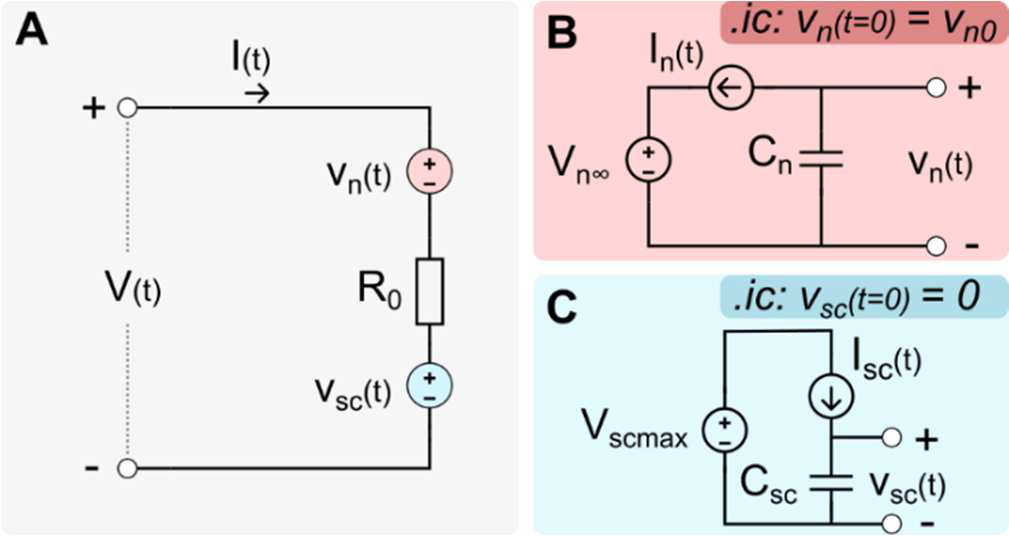
\includegraphics[width=0.8\textwidth]{Chapter5/Figs/d.png}
    \caption[Empirical SPICE Model diagram.]{Empirical SPICE Model diagram. (A) The SPICE model produces an output current, $I(t)$, given an input voltage, $V(t)$. The circuit consists of a single resistor, $R_0$, in addition to two voltage sources which act to reduce or increase the magnitude of the voltage applied to the resistor. These voltage sources are described by the sub-circuits highlighted in blue and red. (B) The voltage source, $V_n(t)$, has an initial value of $V_{n0}$ and reduces over time leading to an increase in device current. (C) In contrast, the voltage source $V_{sc}(t)$ has an initial value of $0V$ and increases over time causing a reduction in the current flowing through the device. All capacitors are set to a value of $1F$, whereas the values of the resistors and voltage biases are obtained from fitting the experimental data.}
    \label{fig:5d}
\end{figure}


\noindent The accelerated rise in conduction appears to be attributable to the phenomenon of charge trapping. This is corroborated by its shorter timescales, greater volatility, and experiments in which optically injected carriers were demonstrated to accelerate the process. One potential mechanism by which charge trapping affects device conductance is through modulation of the height of a Schottky-like barrier \cite{cowley1965surface}, which may be influenced by the population of interface states \cite{sze2021physics}. \\

\noindent Although Schottky barriers are typically formed between metal-semiconductor interfaces, studies have identified analogous barriers within memristor devices \cite{hansen2015double}. The silicon oxide devices exhibit rectifying behaviour, indicating the presence of an interface barrier at one of the metal-insulator interfaces. Additionally, the filaments in the devices are composed of silicon-rich regions within the oxide, suggesting that the interface between these filaments and metal contacts may resemble a Schottky interface.\\

% \noindent The Schottky barrier is modelled as a voltage drop, which acts to reduce the voltage across the active layer of the device, as illustrated in \ref{fig:5d}. As the height of the Schottky barrier diminishes, the potential across the active layer increases, resulting in a greater device current. The voltage drop resulting from the Schottky-like barrier is a function of time and is modelled using the sub-circuit illustrated in red in \ref{fig:5d}. \\

% \noindent The magnitude of the voltage drop is represented within the sub-circuit by the voltage across the capacitor, $C_n$. The initial value of the aforementioned variable is discharged by the current source, $V_{n0}$. The rate of discharge is defined by the current source, $I_n(t)$, whose magnitude is proportional to the difference between the current voltage drop across the Schottky barrier and its final equilibrium value, $V_{n\infty}$.

\noindent The Schottky barrier is modeled as a voltage drop, which acts to reduce the voltage across the active layer of the device, as illustrated in Figure \ref{fig:5d}. As the height of the Schottky barrier diminishes, the potential across the active layer increases, resulting in a greater device current. The voltage drop resulting from the Schottky-like barrier is a function of time and is modeled using the sub-circuit illustrated in red in Figure \ref{fig:5d}. The magnitude of the voltage drop is represented within the sub-circuit by the voltage across the capacitor, $C_n$. The initial value of the aforementioned variable is discharged by the current source, $V_{n0}$. The rate of discharge is defined by the current source, $I_n(t)$, whose magnitude is proportional to the difference between the current voltage drop across the Schottky barrier and its final equilibrium value, $V_{n\infty}$, as defined in Equation (\ref{eq:5.5}).
\begin{align}
I_n(t) = \alpha \times \left[ V_n(t) - V_{n\infty} \right] \label{eq:5.5} 
\end{align}

% \noindent In this equation, $\alpha$ corresponds to the probability of trapping a carrier, while the voltage difference relates to the concentration of unpopulated states. The current source discharges the capacitor to a final equilibrium voltage, $V_{n\infty}$, where the trapping and de-trapping currents are equal. An additional leaking resistor, $R_{leak}$, is introduced to correctly adjust for the rectifying behaviour of the device.\\

\noindent In this equation, $\alpha$ corresponds to the probability of trapping a carrier, while the voltage difference relates to the concentration of unpopulated states. The current source discharges the capacitor to a final equilibrium voltage, $V_{n\infty}$, where the trapping and de-trapping currents are equal. An additional leaking resistor, $R_{leak}$, is introduced to correctly adjust for the rectifying behavior of the device.\\

% \noindent There is compelling evidence that the observed decline in conductance can be attributed to the movement of charged ions within the oxide thin film. This hypothesis has been put forth in the majority of publications on such current transients \cite{wang2006oxygen}. This is largely based on the observation that the decay in conductance occurs over a time scale of tens to hundreds of seconds, which is too long to be associated with the trapping of electrons or holes. \\

% \noindent Furthermore, in accordance with the drifting defect hypothesis, it has been demonstrated that the process can be reversed by applying a voltage of opposite polarity, despite the device exhibiting significantly reduced currents in the opposite polarity. The model adhere to this approach and hypothesise the presence of migrating defects. Of particular significance is the assumption that the ionic current induced by the migrating space charge is negligible in comparison to the electronic currents, as predicted \cite{meyer2005oxygen}. \\

\noindent There is compelling evidence that the observed decline in conductance can be attributed to the movement of charged ions within the oxide thin film. This hypothesis has been put forth in the majority of publications on such current transients \cite{wang2006oxygen}. This is largely based on the observation that the decay in conductance occurs over a time scale of tens to hundreds of seconds, which is too long to be associated with the trapping of electrons or holes. \\

\noindent Furthermore, in accordance with the drifting defect hypothesis, it has been demonstrated that the process can be reversed by applying a voltage of opposite polarity, despite the device exhibiting significantly reduced currents in the opposite polarity. The model adheres to this approach and hypothesizes the presence of migrating defects. Of particular significance is the assumption that the ionic current induced by the migrating space charge is negligible in comparison to the electronic currents, as predicted \cite{meyer2005oxygen}.\\

% \noindent It is assumed that the electronic current flows through a conductive channel within the oxide. In our silicon oxide devices, this is a silicon-rich filament that forms during electrical stressing. Such filaments are common in memristors and have been observed in our devices using etching C-AFM techniques \cite{buckwell2015conductance}.\\

% \noindent In order for an electronic current to be induced through these filaments, it is necessary that a potential be present across the channel. In our model, the migrating space charge modulates the current by reducing the potential experienced along the filament. It is probable that this space charge is a positively charged ion that has accumulated in proximity to the upper gold electrical contact. This assertion is corroborated by the observation that the impact of the accumulation of space charge can be negated by modifying the material of the top electrical contact from gold to indium tin oxide \cite{mannion2022current}.\\

\noindent It is assumed that the electronic current flows through a conductive channel within the oxide. In our silicon oxide devices, this is a silicon-rich filament that forms during electrical stressing. Such filaments are common in memristors and have been observed in our devices using etching C-AFM techniques \cite{buckwell2015conductance}. For an electronic current to be induced through these filaments, a potential across the channel is necessary. In this model, the migrating space charge modulates the current by reducing the potential experienced along the filament. This space charge is probably a positively charged ion that has accumulated in proximity to the upper gold electrical contact. This assertion is corroborated by the observation that the impact of the accumulation of space charge can be negated by modifying the material of the top electrical contact from gold to indium tin oxide \cite{mannion2022current}.\\

% \noindent The precise nature of this ion remains uncertain. A substantial amount of oxygen migration and associated oxygen vacancies have been observed throughout the device when under bias \cite{vanka2022hydrogen}, indicating that this could be a viable candidate. However, in other devices, hydrogen has been identified as a defining factor in device behaviour. Additionally, hydrogen has been detected in significant quantities within our devices \cite{lagarias1998convergence}. Given the lack of certainty regarding the identity of the ion, we assume a generic space charge.\\

\noindent The precise nature of this ion remains uncertain. A substantial amount of oxygen migration and associated oxygen vacancies have been observed throughout the device when under bias \cite{vanka2022hydrogen}, indicating this could be a viable candidate. However, in other devices, hydrogen has been identified as a defining factor in device behavior. Additionally, hydrogen has been detected in significant quantities within our devices \cite{lagarias1998convergence}. Given the lack of certainty regarding the identity of the ion, a generic space charge is assumed.\\

% \noindent The effect of the space charge on the conductive channel can be described as follows. In the initial phase, the space charge exhibits a homogeneous distribution. Upon the application of a voltage to the device, a force is imparted on the space charge, resulting in its drift and accumulation at the device electrode. This accumulation effectively blocks the space charge from exiting the oxide.  \\

% \noindent This accumulation results in the formation of a region of higher space charge concentration, which consumes a portion of the potential applied across the device. This results in a reduction in the potential drop across the conductive channel. As the space charge accumulates, this voltage drop increases, meaning less potential is dropped across the channel and a reduction in device current is observed. \\

% \noindent Eventually, the drifting force imparted on the space charge will reach equilibrium with the diffusion and Coulombic repulsion formed by the accumulated space charge, leading to a steady state condition. When the potential is removed, the space charge diffuses back to its original distribution. \\

\noindent The effect of the space charge on the conductive channel can be described as follows. In the initial phase, the space charge exhibits a homogeneous distribution. Upon the application of a voltage to the device, a force is imparted on the space charge, resulting in its drift and accumulation at the device electrode. This accumulation effectively blocks the space charge from exiting the oxide. This accumulation results in the formation of a region of higher space charge concentration, which consumes a portion of the potential applied across the device. This leads to a reduction in the potential drop across the conductive channel. As the space charge accumulates, this voltage drop increases, meaning less potential is dropped across the channel and a reduction in device current is observed. Eventually, the drifting force imparted on the space charge will reach equilibrium with the diffusion and Coulombic repulsion formed by the accumulated space charge, leading to a steady-state condition. When the potential is removed, the space charge diffuses back to its original distribution.\\

% \noindent The aforementioned process is modelled using the circuit illustrated in Figure \ref{fig:5d}. The conductive channel is represented by a fixed resistance, designated as $R_0$. The voltage across the conductive channel is defined by the applied potential at the terminals of the device, $V(t)$, and the voltage source, $V_{sc}(t)$, which represents the voltage drop caused by the accumulated space charge. This voltage source is time-dependent and is defined by the subcircuit shown in blue. As the voltage of this source increases over time, the voltage across the fixed resistor drops and the device current also reduces.

\noindent This process is modeled using the circuit illustrated in Figure \ref{fig:5d}. The conductive channel is represented by a fixed resistance, designated as $R_0$. The voltage across the conductive channel is defined by the applied potential at the terminals of the device, $V(t)$, and the voltage source, $V_{sc}(t)$, which represents the voltage drop caused by the accumulated space charge. This voltage source is time-dependent and is defined by the subcircuit shown in blue. As the voltage of this source increases over time, the voltage across the fixed resistor drops, and the device current also reduces.
\begin{align}
I_{sc}(t) = \left[ V_{scmax} - V_{sc}(t) \right] \times \left[ \mu \left( V(t) - V_{sc}(t) \right) \right] \label{eq:5.6} 
\end{align}

% \noindent As illustrated in Figure \ref{fig:5d}C, the sub-circuit meticulously monitors the accumulation of the space charge and its concomitant voltage drop. The voltage across the capacitor is represented by the voltage drop. The charging of the capacitor is effected by the current source $I_{sc}(t)$, the result being the generation of a current in accordance with equation \ref{eq:5.6}. The term is defined by the voltage applied across the device and $\mu$, which symbolises the mobility of the space charge. The current source is able to draw charge from a voltage source, which represents the steady-state voltage drop. That is to say, the maximum voltage drop consumed by the accumulated space charge $V_{scmax}$.

\noindent As illustrated in Figure \ref{fig:5d}C, the sub-circuit meticulously monitors the accumulation of the space charge and its concomitant voltage drop. The voltage across the capacitor represents this voltage drop. The charging of the capacitor is effected by the current source $I_{sc}(t)$, which generates a current in accordance with Equation (\ref{eq:5.6}). The term is defined by the voltage applied across the device and $\mu$, which symbolizes the mobility of the space charge. The current source is able to draw charge from a voltage source, representing the steady-state voltage drop, i.e., the maximum voltage drop consumed by the accumulated space charge $V_{scmax}$.

\section[Composite Empirical Formulation]{Composite Empirical Formulation}

% \noindent To complete the model, the subcircuits for both potential drops are combined as illustrated in Fig \ref{fig:5d}. The two voltage drops act upon a single resistor representing the conductive channel, $R_0$. In practice, this channel does not exhibit ohmic conduction and thus its resistance will have a voltage dependence. This is taken into account while collecting the meta-parameters.

\noindent To complete the model, the subcircuits for both potential drops are combined, as illustrated in Figure \ref{fig:5d}. The two voltage drops act upon a single resistor representing the conductive channel, $R_0$. In practice, this channel does not exhibit ohmic conduction, and thus its resistance will have a voltage dependence. This non-ohmic behavior is taken into account while collecting the meta-parameters.

\subsection[Parameter Fitting]{Parameter Fitting}

\begin{table}[ht]
    \caption{Model parameter values.}
    \centering
    \begin{tabular}{|c|c|c|}
    \hline
    Parameter   & Function                & Value                                      \\ \hline
    $R_0$       & Exponential             & $R_0(V) = 6.00 \times 10^6 \cdot exp(-1.07V)$         \\ \hline
    $\alpha$    & Linear                  & $\alpha(V) = 1.09V -0.454$                 \\ \hline
    $V_{n\infty}$ & Constant                & $V_{n\infty} = 0.35$                         \\ \hline
    $V_{n0}$    & Linear                  & $V_{n0}(V) = 1.03V - 0.391 $               \\ \hline
    $\mu$       & Second Order Polynomial & $\mu(V) = -0.038V^2 + 0.142V - 0.057$      \\ \hline
    $V_{scmax}$ & Exponential             & $V_{scmax}(V) = 5.17 \times 10^{-2} \cdot exp(2.01V)$ \\ \hline
    \end{tabular}
    \label{table:5b}
\end{table}

% \noindent The complete model comprises six parameters, which are listed in Table \ref{table:5b}. These parameters will be fitted to the dataset plotted, which shows the current transients observed in a single device at various voltages ranging from 0.7 V to 1.1 V.\\

% \noindent Initially, the model is individually fit to each voltage trial and will then be generalised in a later stage. Fitting is carried out in MATLAB using the \texttt{fminsearch} function which employs the simplex search method \cite{lagarias1998convergence} to minimise an error function which has been set to the mean-squared-error. \\

\noindent The complete model comprises six parameters, which are listed in Table 5.2. These parameters were fitted to a dataset showing the current transients observed in a single device at various voltages ranging from 0.7V to 1.1V. Initially, the model was individually fit to each voltage trial and later generalized. Fitting was carried out in MATLAB using the \texttt{fminsearch} function, which employs the simplex search method \cite{lagarias1998convergence} to minimize an error function set to the mean-squared-error.\\

% \noindent The process of fitting individual voltage trials results in a set of parameters which exhibit voltage dependencies except for one exception, $V_{n\infty}$, which is spread around a central value for different voltages and so is assumed to be independent of the applied voltage. For this parameter we calculate the mean average of its value across the dataset and then set it as constant, 0.35V.\\

\noindent The process of fitting individual voltage trials resulted in a set of parameters that exhibit voltage dependencies, with one exception: $V_{n\infty}$. This parameter was found to be distributed around a central value for different voltages and was therefore assumed to be independent of the applied voltage. For $V_{n\infty}$, the mean average of its value across the dataset was calculated and set as a constant, 0.35V.\\

\begin{figure}[htbp!] 
    \centering    
    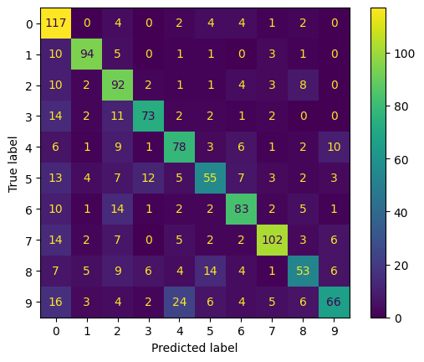
\includegraphics[width=1\textwidth]{Chapter5/Figs/e.png}
    \caption[Fitting performance of the SPICE model.]{Fitting performance of the SPICE model. (A) The model’s response is compared with experimental data for a range of voltages. Experimental datapoints are indicated with gray points while model predictions are plotted with solid coloured lines. For each voltage case, the parameters in table \ref{table:5b} are refitted to minimise the mean-squared-error between the experimental and model's response. (B) The residuals between the model's prediction and experimental data is plotted for $V=0.7V$  which exhibits the largest error of 13\% at the onset of the transient which is predominantly due to noise within the experimental data. In contrast, the average percentage difference for the duration of the transient is 2\% with absolute residuals never exceeding $5nA$.}
    \label{fig:5e}
\end{figure}

% \noindent The prediction of the model when parameters are reoptimised for each specific voltage case is plotted in Fig. 3A. As illustrated in Figure 3B, an example residual for the case of 0.7 V is presented. This figure demonstrates the presence of suboptimal residuals, attributable to the diminished device currents. It is noteworthy that a maximum error of 13\% is exhibited at the transient's onset. Nevertheless, these errors decrease quickly, resulting in a mean error of only 1.9\% over the duration of the transient. \\

% \noindent For all voltage cases, the absolute error remains less than 5nA throughout the transient. This appears to be a reasonable fit. However, a persistent oscillation is observed in the residuals of all voltage cases, suggesting that the model is missing some dynamics within the current transient. It is evident that this approach to fitting will result in an optimal fit, owing to the re-optimisation of parameters for each voltage case. \\

% \noindent It should be noted that the model has not yet been generalised. In its present state, it is necessary to modify the SPICE model's parameters in accordance with the voltage applied to the device. The ideal scenario would involve the development of a generalized model, in which a single set of parameters is applicable to a range of applied voltages.\\

\noindent The prediction of the model when parameters are reoptimized for each specific voltage case is plotted in Figure \ref{fig:5d}A. As illustrated in Figure \ref{fig:5d}B, an example residual for the case of 0.7V is presented. This figure demonstrates the presence of suboptimal residuals, primarily attributable to the diminished device currents and noise within the experimental data. A maximum error of 13\% is exhibited at the transient's onset. Nevertheless, these errors decrease quickly, resulting in a mean error of only 1.9\% over the duration of the transient. For all voltage cases, the absolute error remains less than 5nA throughout the transient, indicating a reasonable fit. \\

\noindent However, a persistent oscillation is observed in the residuals of all voltage cases, suggesting that the model is missing some dynamics within the current transient. It is evident that this approach to fitting will result in an optimal fit, owing to the re-optimization of parameters for each voltage case. It should be noted that the model had not yet been generalized. In its initial state, it was necessary to modify the SPICE model's parameters in accordance with the voltage applied to the device. The ideal scenario involved the development of a generalized model, in which a single set of parameters is applicable to a range of applied voltages.\\

\begin{figure}[htbp!] 
    \centering    
    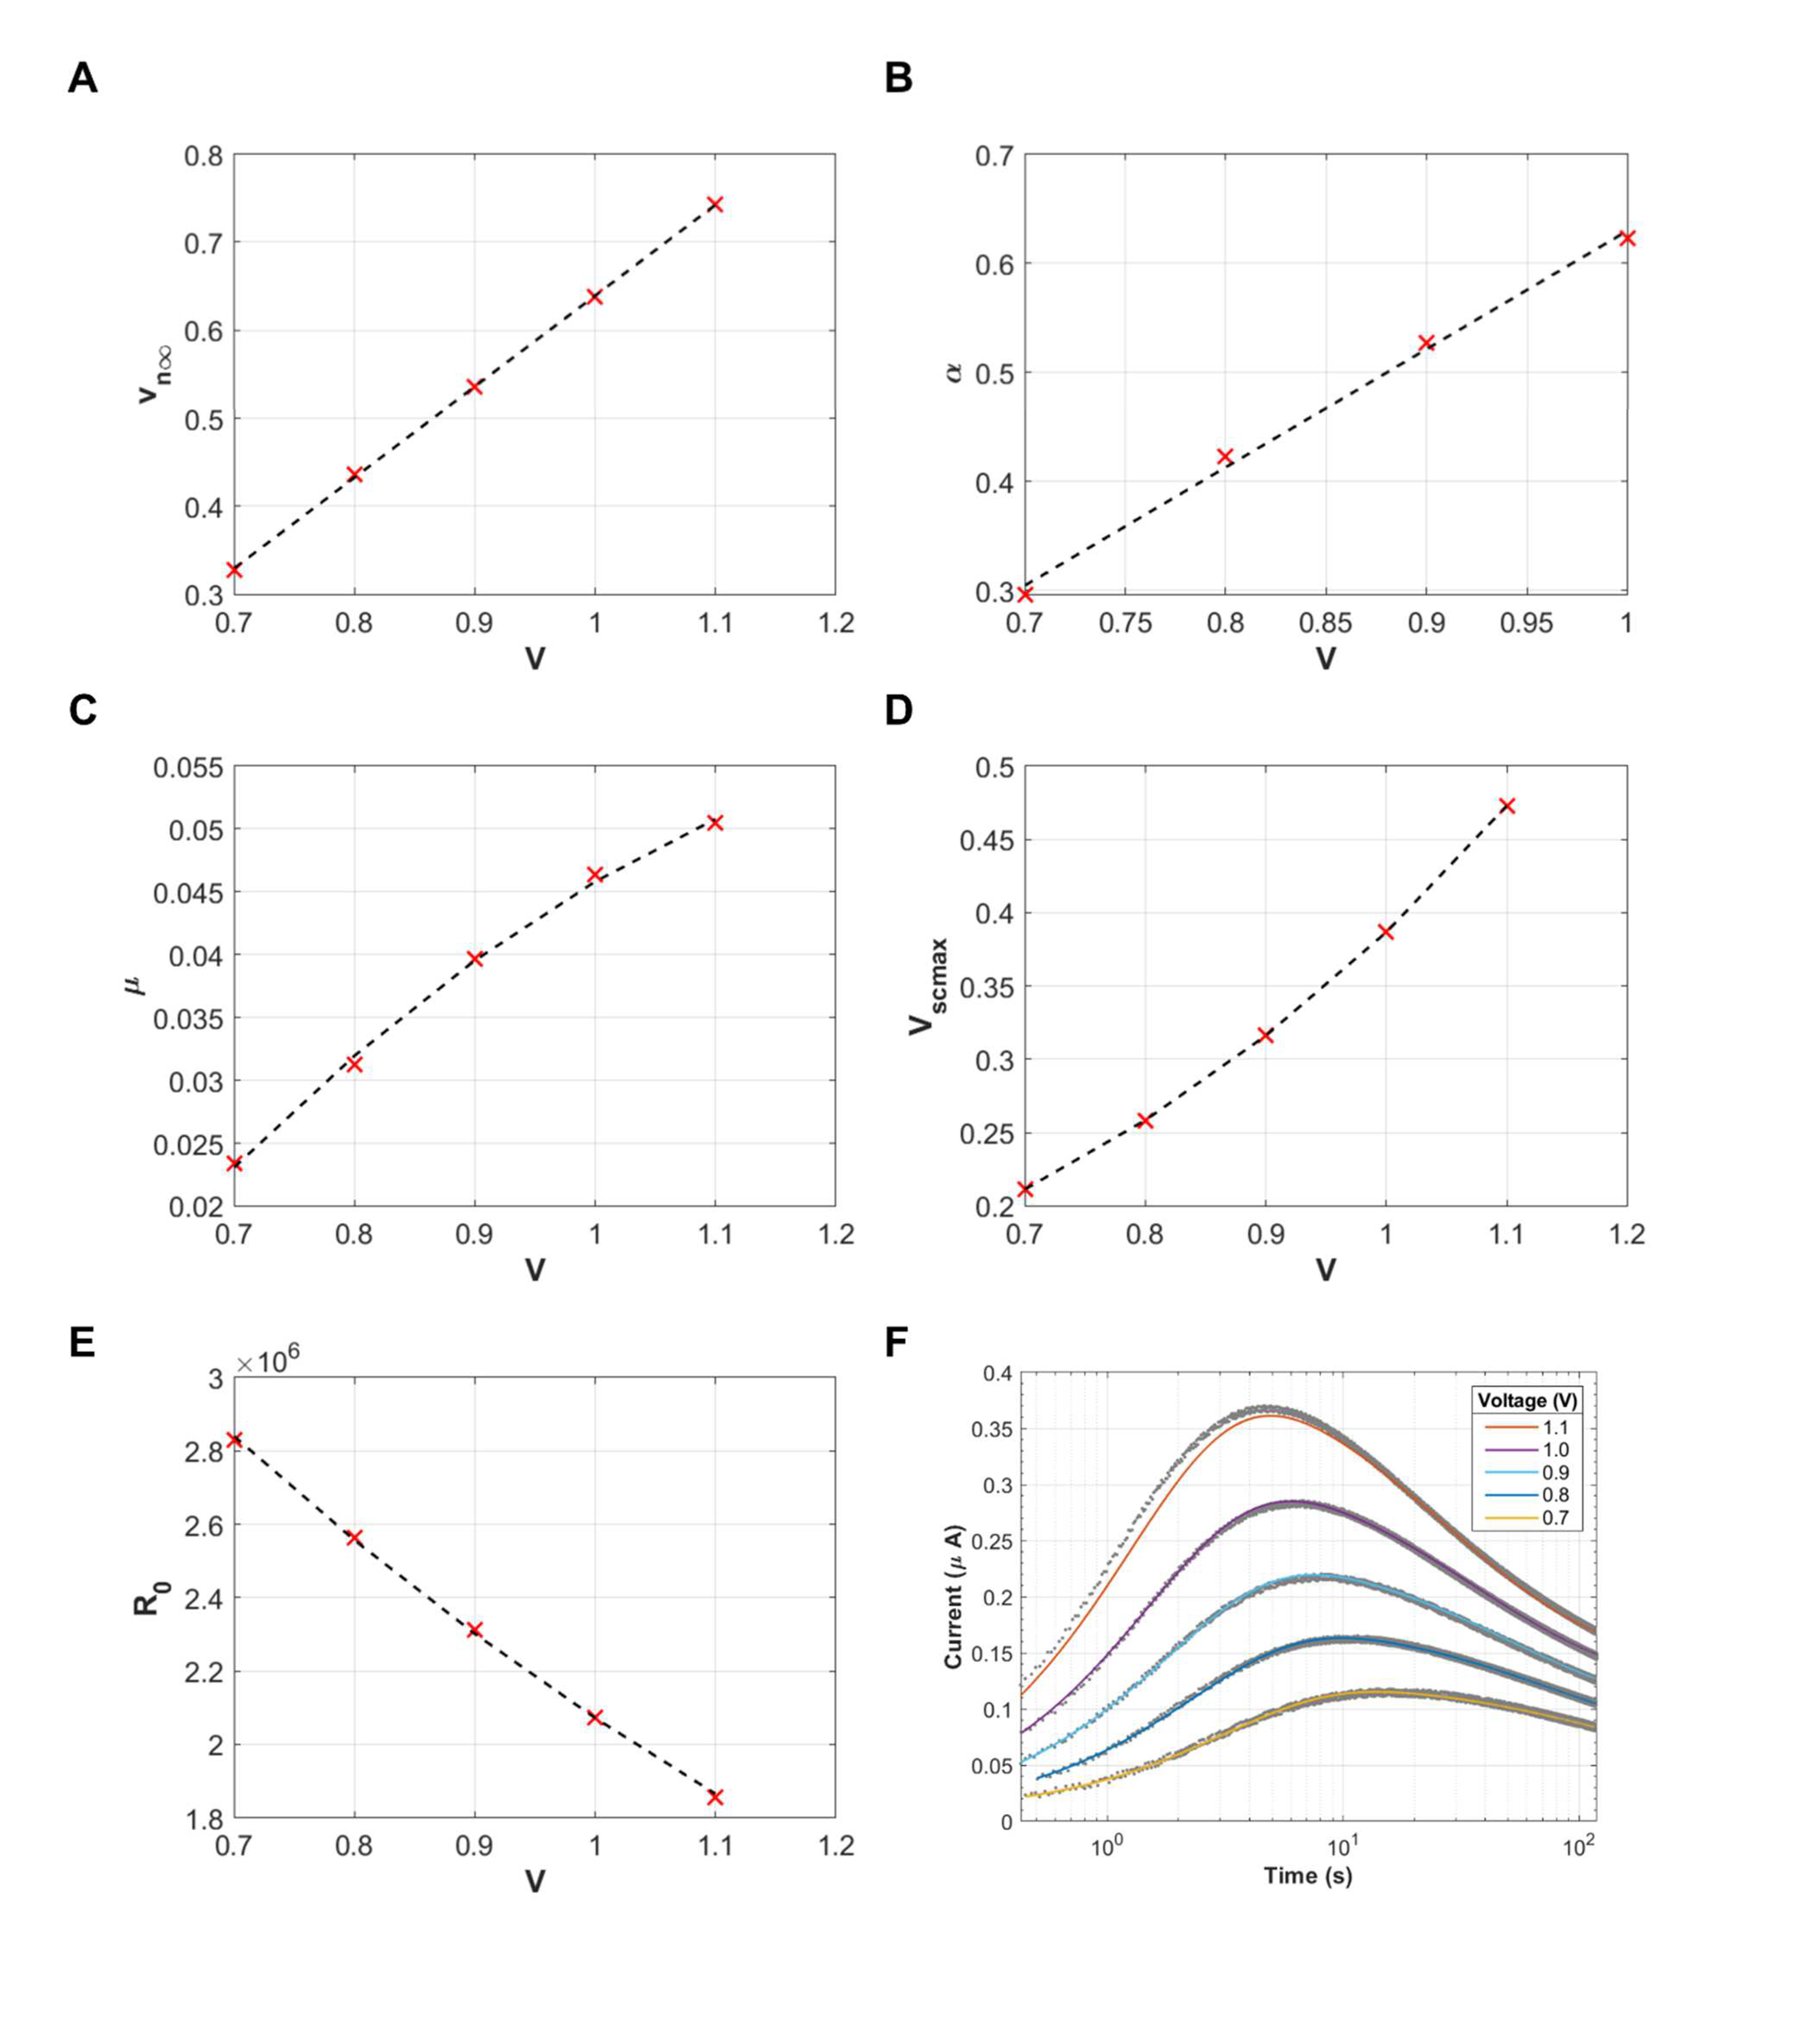
\includegraphics[width=1\textwidth]{Chapter5/Figs/f.png}
    \caption[Fitting of the model's meta-parameters.]{Fitting of the model's meta-parameters. (A-E) The fitting for each of the model's parameters is plotted using the equations described in Table \ref{table:5b}. These functions' coefficients are referred to as meta-parameters and are used in the generalised model to produce a black box model that reproduces the current-time response to any voltage between 0.7 and 1.0 V. (F) The generalised model's response is plotted alongside the experimental data. This model uses the previously described meta-parameters. However, the generalised model breaks down at larger voltages, i.e. at 1.1 V. We assume this is due to the additional stressing of the oxide that occurs at higher voltages and device currents.}
    \label{fig:5f}
\end{figure}

% \noindent In order to generalise the model, it is necessary to modify it in order to account for the voltage dependency of each parameter. It is inevitable that this process will introduce error into the model's behaviour and increase fitting residuals. Nevertheless, the capacity to predict device behaviour over a range of voltages using a single set of parameters justifies this reduction in accuracy. \\

% \noindent For each of the voltage-dependent parameters, the parameter values are fitted to a suitable function, as indicated in Table \ref{table:5b} and illustrated in Fig. \ref{fig:5f}A-E. The extraction of the coefficients that describe the voltage dependency, for example the gradient and offset of a single order polynomial, is achieved from these functions. The term 'meta-parameters' is employed to denote these coefficients, as they encompass the parameters obtained previously from fitting the experimental data.\\

\noindent To generalize the model, it was necessary to account for the voltage dependency of each parameter. While this process inevitably introduces some error into the model's behavior and increases fitting residuals, the capacity to predict device behavior over a range of voltages using a single set of parameters justifies this reduction in accuracy. For each of the voltage-dependent parameters, the parameter values were fitted to a suitable function, as indicated in Table \ref{table:5b} and illustrated in Figure \ref{fig:5f}A-E. The extraction of the coefficients that describe the voltage dependency (e.g., the gradient and offset of a single order polynomial) was achieved from these functions. The term 'meta-parameters' is employed to denote these coefficients, as they encompass the parameters obtained previously from fitting the experimental data.\\

% \noindent The predictions of the generalised model are illustrated in Figure \ref{fig:5f}F. The discrepancies between the experimental and simulated device currents for each voltage curve have increased in comparison to the voltage-specific parameters. However, the advantage of the generalised model is that its parameters no longer require refitting for different applied voltages.\\

% \noindent A substantial departure from the established model is observed for the case of 1.1V. As demonstrated in Figure \ref{fig:5f}F, the model reliably forecasts a reduced device current during the initial phase of the transient. This phenomenon can be attributed to the elevated applied voltage and the resultant currents, which induce electrical stress within the oxide. \\

% \noindent It has been established that these devices exhibit an increase in conductivity in response to electrical stress \cite{mannion2023unipolar}. This can be rectified by the introduction of a stressing term, which serves to augment the number of traps within our representation of the Schottky interface. The discharge current, as outlined in equation \ref{eq:5.5}, is modified to encompass a term that facilitates the charging of the capacitor.

\noindent The predictions of the generalized model are illustrated in Figure \ref{fig:5f}F. The discrepancies between the experimental and simulated device currents for each voltage curve have increased in comparison to the voltage-specific parameters. However, the advantage of the generalized model is that its parameters no longer require refitting for different applied voltages. A substantial departure from the established model is observed for the case of 1.1V. As demonstrated in Figure \ref{fig:5f}F, the model reliably forecasts a reduced device current during the initial phase of the transient. \\

\noindent This phenomenon can be attributed to the elevated applied voltage and the resultant currents, which induce electrical stress within the oxide. It has been established that these devices exhibit an increase in conductivity in response to electrical stress \cite{mannion2023unipolar}. This can be rectified by the introduction of a stressing term, which serves to augment the number of traps within the representation of the Schottky interface. The discharge current, as outlined in Equation (\ref{eq:5.5}), is modified to encompass a term that facilitates the charging of the capacitor.\\
\begin{align}
    I_n(t) = \alpha \times \left[ V_n(t) - V_{n\infty} \right] -\sigma I(t) \label{eq:5.7} 
\end{align}

\noindent This modification is employed to simulate the creation of additional trap sites. The term is proportional to the current flowing through the device, $\sigma$, which represents the probability of defect creation for a given magnitude of current. This process ultimately yields the result depicted in equation \ref{eq:5.7}.\\

\begin{figure}[htbp!] 
    \centering    
    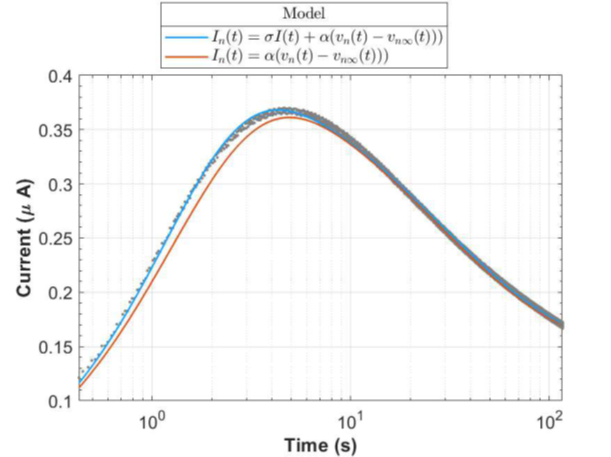
\includegraphics[width=0.6\textwidth]{Chapter5/Figs/g.png}
    \caption[The improvement of SPICE fit at higher voltages.]{The improvement of SPICE fit at higher voltages. Two versions of the The following generalised models are plotted for 1.1 V. As indicated in the legend, the model incorporating an additional stressing term, $\sigma = 5.61 \times 10^5$, demonstrates enhanced performance at elevated voltages in comparison to the model devoid of the stressing term. The necessity for this term can be attributed to the hypothesis that stress is beginning to occur within the oxide at this higher voltage.}
    \label{fig:5g}
\end{figure}

% \noindent The result of introducing this additional stressing term is illustrated in Figure \ref{fig:5g}. The two models are contrasted both with and without the stressing term, and it is evident that the introduction of the stressing term, where $\sigma = 5.61 \times 10^5$, improves the model's performance in the first half of the transient. It is important to note, however, that the model is no longer generalized because this stressing term does not apply to smaller voltages.\\

% \noindent The SPICE model proposed in Figure \ref{fig:5d} can therefore be generalised for silicon dioxide devices for voltage ranges within 0.7V and 1.0V. It is imperative that the model be modified to account for the additional stressing occurring within the oxide. This can be achieved by introducing a stressing term, as outlined in equation \ref{eq:5.7}. Nevertheless, the validity of this stressing term remains unvalidated for voltages in excess of 1.1V. Consequently, it is highly probable that additional modifications will be required to ensure accurate stressing.

\noindent The result of introducing this additional stressing term is illustrated in Figure \ref{fig:5g}. The two models are contrasted, both with and without the stressing term, and it is evident that the introduction of the stressing term, where $\sigma = 5.61 \times 10^5$, significantly improves the model's performance in the first half of the transient. It is important to note, however, that the model is no longer generalized because this stressing term does not apply to smaller voltages. \\

\noindent The SPICE model proposed in Figure \ref{fig:5d} can therefore be generalized for silicon dioxide devices for voltage ranges within 0.7V and 1.0V. It is imperative that the model be modified to account for the additional stressing occurring within the oxide. This can be achieved by introducing a stressing term, as outlined in Equation (\ref{fig:5g}). Nevertheless, the validity of this stressing term remains unvalidated for voltages in excess of 1.1V. Consequently, it is highly probable that additional modifications will be required to ensure accurate stressing at higher operating points.

\subsection[Physical Model Derivation]{Physical Model Derivation}

% \noindent In its current configuration, the model operates within a constrained voltage range to prevent significant electrical stressing of the device. For example, device characterization has been limited to voltages not exceeding 1.1V. If the voltage is increased beyond this threshold, stress-induced effects alter the shape of the current transient, rendering the existing model invalid. The appropriate voltage range can be determined empirically by performing multiple trials at a fixed voltage. If a gradual increase in conductance is observed across trials, it indicates the onset of stressing, and the voltage should be reduced accordingly \\

\noindent In its current configuration, the model operates within a constrained voltage range to prevent significant electrical stressing of the device. For example, device characterization has been limited to voltages not exceeding 1.1V. If the voltage is increased beyond this threshold, stress-induced effects alter the shape of the current transient, rendering the existing model invalid. The appropriate voltage range can be determined empirically by performing multiple trials at a fixed voltage. If a gradual increase in conductance is observed across trials, it indicates the onset of stressing, and the voltage should be reduced accordingly.\\

\begin{figure}[htbp!] 
    \centering    
    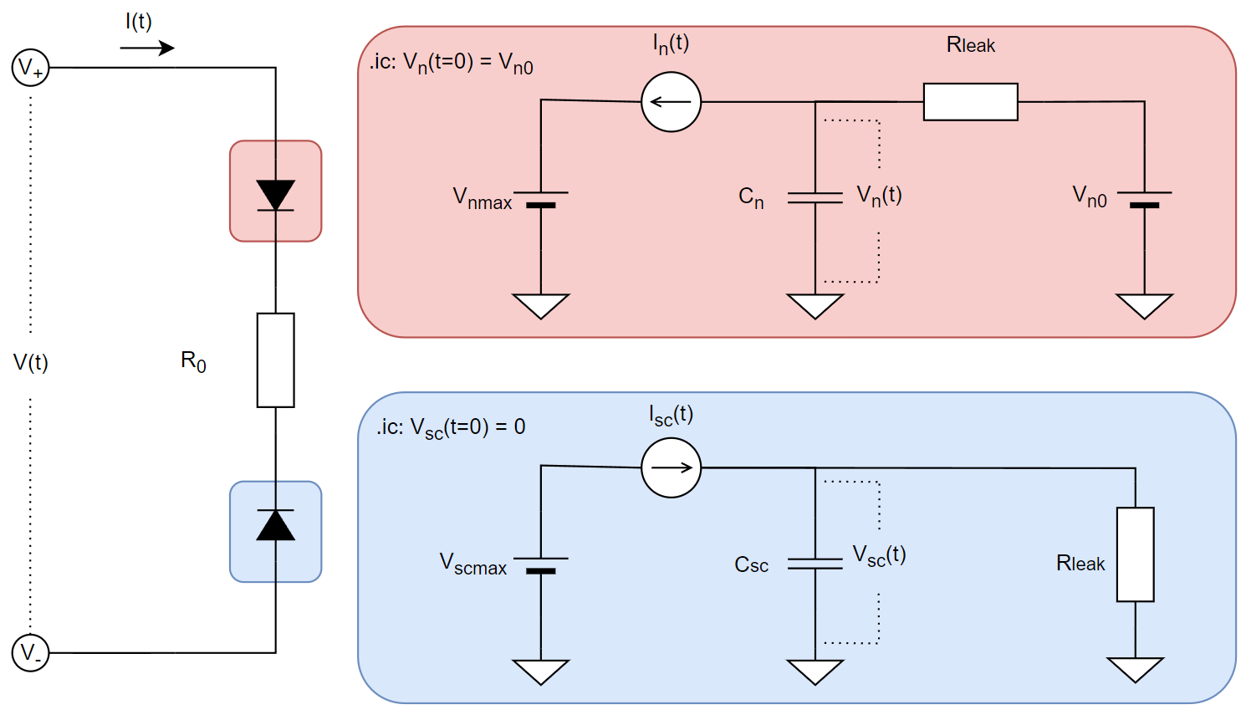
\includegraphics[width=0.9\textwidth]{Chapter5/Figs/h.png}
    \caption[The extended SPICE Model diagram.]{The extended SPICE Model diagram. The improvement of SPICE fit at higher voltages. The SPICE model generates an output current, \textit{I(t)}, based on an input voltage, \textit{V(t)}. The circuit incorporates a single resistor, $R_0$, along with two diode models that serve to attenuate or amplify the voltage applied to the resistor. These diode models are represented by the sub-circuits highlighted in blue and red.}
    \label{fig:5h}
\end{figure}

% \noindent To extend the model’s applicability to more general inputs—beyond simple step potentials—it is essential to account for the relaxation behavior of the current transient. This can be achieved by adding leakage components $R_{leak}$ to the charge-trapping and space-charge subcircuits, allowing their associated capacitors to charge and discharge over time.\\

% \noindent The enhanced model shown in Figure \ref{fig:5h} builds upon earlier designs by replacing static voltage sources with diode-based elements that better replicate Schottky-like metal-insulator contact behavior. It also introduces dynamic relaxation features that emerge when input potentials are removed or the device is grounded.

\noindent To extend the model's applicability to more general inputs—beyond simple step potentials—it is essential to account for the relaxation behavior of the current transient. This can be achieved by adding leakage components$R_{leak}$  to the charge-trapping and space-charge subcircuits, allowing their associated capacitors to charge and discharge over time.\\

\noindent The enhanced model, shown in Figure \ref{fig:5h}, builds upon earlier designs by replacing static voltage sources with diode-based elements that better replicate Schottky-like metal-insulator contact behavior. It also introduces dynamic relaxation features that emerge when input potentials are removed or the device is grounded.
\begin{align}
I_d(t) = \left( I_0 + I_{\delta} V_n(t) \right)\times \left( e^{\frac{V(d_1,d_2)}{nV_t} }  - 1\right) \label{eq:5.8}
\end{align}

\noindent Where $I_d(t)$ is the time-dependent diode current, which captures how the current evolves over time due to transient phenomena or dynamic voltage input. $I_0$ is the reverse saturation current or the leakage current through the diode when reverse-biased. It is an intrinsic property of the junction and depends on factors like material properties and temperature. \\

\noindent $I_{\delta} V_n(t)$ is the modulated current term, a dynamic extension not present in the standard Shockley equation. It introduces a time-varying modulation of the saturation current, where $I_{\delta}$ is a scaling factor representing sensitivity of the diode to input modulation and $V_n(t)$ is a time-dependent voltage signal driven from an internal node. Together this term allows the diode behavior to adapt dynamically to changes in the input signal, which is crucial for modeling transient memristive phenomena such as relaxation and adaptation.\\

\noindent $V(d_1,d_2)$ Voltage difference across the diode terminals in the SPICE model. This is equivalent to the V in the traditional Shockley equation. This voltage controls the exponential response of the diode. $n$ Ideality factor that reflects how closely the diode follows the ideal Shockley behavior. An $n>1$ accounts for recombination losses or non-idealities in real diodes and is often used to better fit experimental data. Finally, $V_t$ is the thermal voltage.\\

\noindent To derive a form that better matches experimentally observed transient behavior from the original (\ref{eq:5.5}), it is assumed that $V_{n\infty} = V_{scmax}$, a simplification that assumes both voltages reflect the same saturation point for field-driven relaxation. Moreover, since the decay dynamics of $V_n(t)$ are influenced by the total device current, a modulation term by the main current $I_d(t)$ from (\ref{eq:5.8}) is introduced, leading to the modified expression:
\begin{equation}
I_n(t) = \alpha I_d(t) \left[ V_{scmax} - V_n(t) \right] \label{eq:5.9}
\end{equation}
This equation captures both the deviation from equilibrium and the feedback from the instantaneous device current, providing a more accurate representation of the charge relaxation behavior observed in subthreshold memristive devices. To simplify the original space-charge current (\ref{eq:5.6}) expression for modeling in SPICE, the voltage driving the ionic drift as the terminal voltage is approximated as $V(d_1, d_2)$. Additionally, the modulation term $\left[ V_{scmax} - V_{sc}(t) \right]$ can be treated as constant or absorbed into the mobility factor $\mu$ in certain operating regimes. This leads to the simplified form:
\begin{equation}
I_{sc}(t) = \mu V_{sc}(t) \cdot V(d_1, d_2) \label{eq:5.10}
\end{equation}
% which effectively captures the relationship between accumulated space charge potential and the applied terminal bias. These modified equations are better suited for implementation in compact SPICE models used to simulate transient behavior in neuromorphic circuits. 

\noindent This simplified form effectively captures the relationship between accumulated space charge potential and the applied terminal bias. These modified equations are better suited for implementation in compact SPICE models used to simulate transient behavior in neuromorphic circuits.

\begin{table}[ht]
    \caption{Extemded model parameter values.}
    \centering
    \begin{tabular}{|c|c|c|}
    \hline
    Parameter   & Function                & Value                                      \\ \hline
    $I_0$       & Exponential             & $I_0(V) = 2.39\times10^{-9}\cdot e^{-13.4V} + 1.03\times 10^{-13}\cdot e^{-1.53V}$         \\ \hline
    $I_{\delta}$    & Power                  & $I_{\delta}(V)=7.41\times 10^{-15} \cdot V^{-2.91}$                 \\ \hline
    $n$ & Polynomial                & $n(V)=-0.131V^2 + 1.01V + 0.615$                         \\ \hline
    \end{tabular}
    \label{table:5c}
\end{table}

% \noindent The initial equation fitting for each trial yielded small residuals, indicating a satisfactory fit, albeit only within the noise range and limited to individual voltages. The model was then generalised, with parameters plotted across various voltages. This resulted in a set of empirical functions (hyperparameters) that account for voltage dependency in table \ref{table:5c}. This approach facilitates the simulation of blackbox circuits and consequently identifies novel diode parameters that augment the previous model's fit, as seen in Figure \ref{fig:5i}.\\

\begin{figure}[htbp!] 
    \centering    
    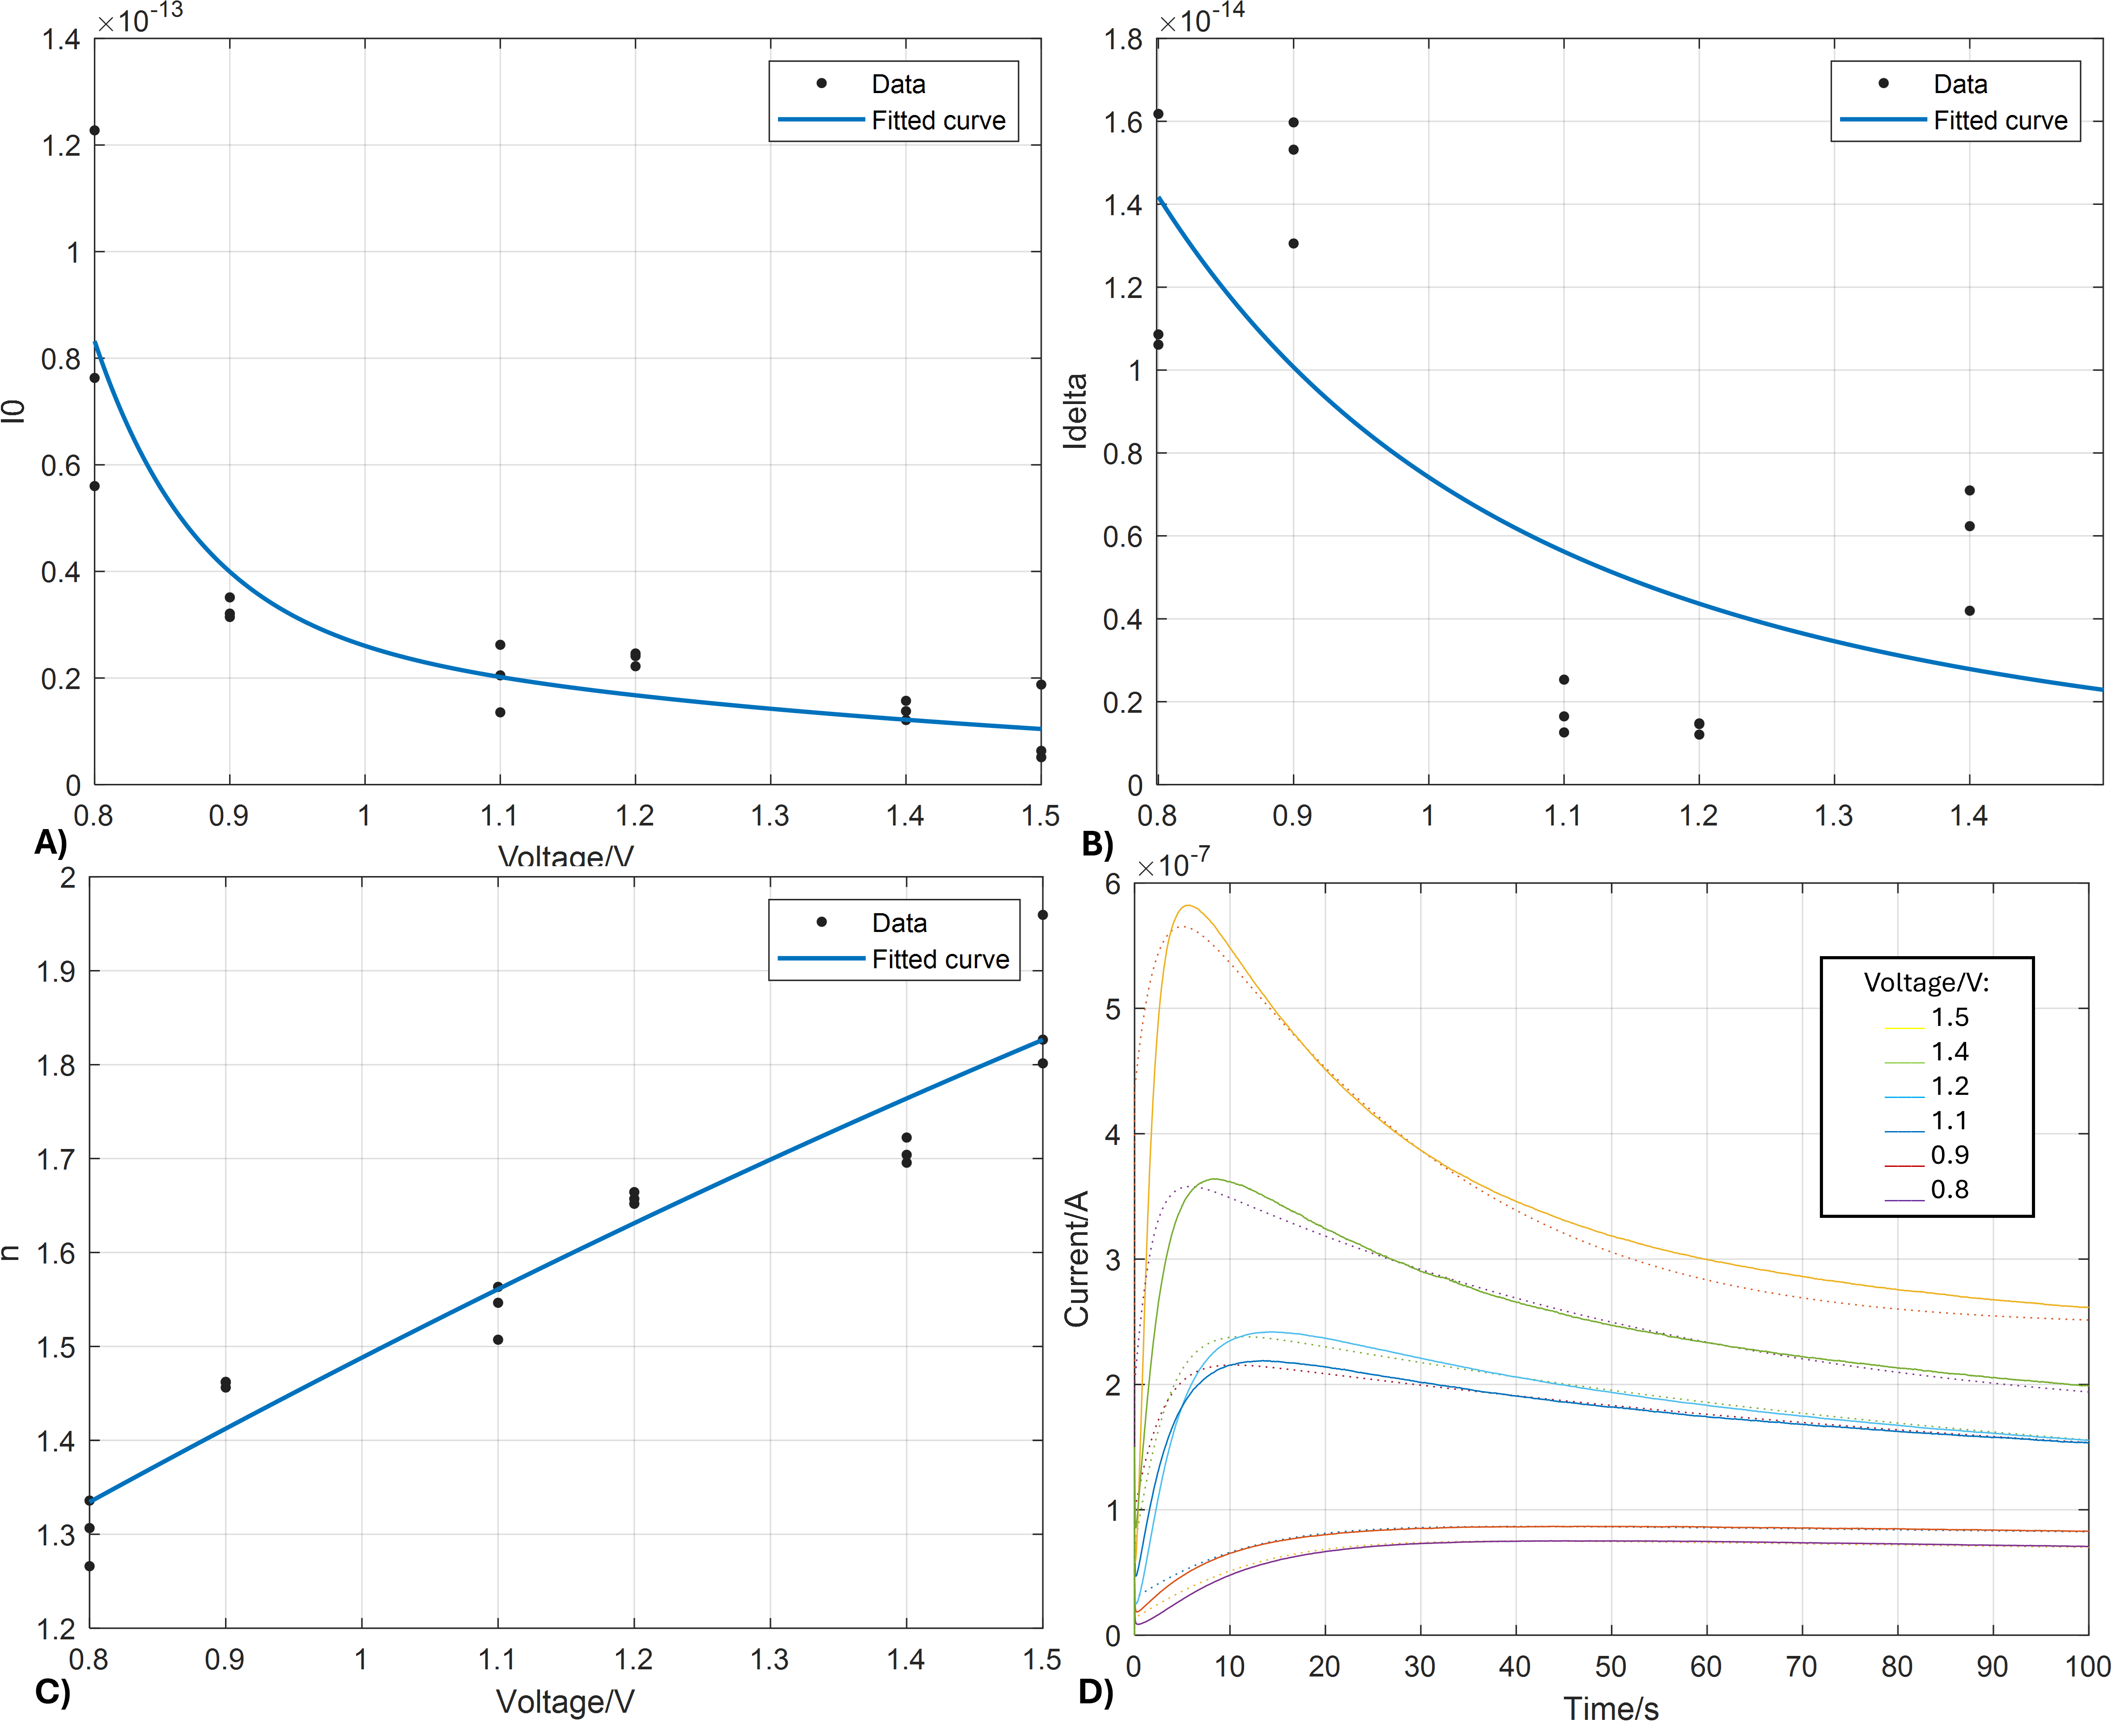
\includegraphics[width=0.9\textwidth]{Chapter5/Figs/i.png}
    \caption[Fitting of the extended model's meta-parameters.]{Fitting of the extended model's meta-parameters. (A-C) The fitting for each of the model's parameters is plotted using the equations described in Table \ref{table:5c} that reproduces the current-time response at higher voltage. (D) The generalised model's response is plotted alongside the experimental data from 0.8V to 1.5V.}
    \label{fig:5i}
\end{figure}

\noindent The initial equation fitting for each trial yielded small residuals, indicating a satisfactory fit, albeit only within the noise range and limited to individual voltages. The model was then generalized, with parameters plotted across various voltages. This resulted in a set of empirical functions (hyperparameters) that account for voltage dependency, as shown in Table \ref{table:5c}. This approach facilitates the simulation of blackbox circuits and consequently identifies novel diode parameters that augment the previous model's fit, as seen in Figure \ref{fig:5i}.\\

% \noindent Finally, Figure \ref{fig:5j} illustrates the behavior of the extended SPICE model incorporating relaxation dynamics, particularly under pulsed input conditions. Each pulse generates a sharp rise in current followed by a decay, reflecting the transient response of charge trapping and space-charge mechanisms.\\

% \noindent Over successive pulses, the peak current gradually decreases, demonstrating the cumulative effect of relaxation when the step potential is removed between pulses. This decay mirrors experimentally observed behaviors in memristive devices operating in the subthreshold regime, where ionic and electronic processes relax during the off periods. The extended model captures this temporal evolution, offering improved accuracy for simulating pulsed neuromorphic stimuli.

\begin{figure}[htbp!] 
    \centering    
    \includegraphics[width=0.6\textwidth]{Chapter5/Figs/j.png}
    \caption[Simulated current transient response under repeated voltage pulses using the extended SPICE model.]{Simulated current transient response under repeated voltage pulses using the extended SPICE model. The gradual decay in peak current illustrates the relaxation dynamics of charge trapping and space-charge effects when step potentials are intermittently removed, consistent with subthreshold memristive behavior.}
    \label{fig:5j}
\end{figure}

\noindent Finally, Figure \ref{fig:5j} illustrates the behavior of the extended SPICE model incorporating relaxation dynamics, particularly under pulsed input conditions. Each pulse generates a sharp rise in current followed by a decay, reflecting the transient response of charge trapping and space-charge mechanisms. Over successive pulses, the peak current gradually decreases, demonstrating the cumulative effect of relaxation when the step potential is removed between pulses. This decay mirrors experimentally observed behaviors in memristive devices operating in the subthreshold regime, where ionic and electronic processes relax during the off periods. The extended model captures this temporal evolution, offering improved accuracy for simulating pulsed neuromorphic stimuli.


\section[Summary]{Summary}

% \noindent This chapter has introduced a comprehensive framework for modeling current transients in silicon oxide-based memristive devices, with a particular focus on their relevance to neuromorphic applications. A key finding is the discovery that modifying the top electrode material—specifically, replacing gold with indium tin oxide (ITO)—leads to a significant change in transient behavior. \\

% \noindent While gold-contacted devices exhibit both the characteristic increase and subsequent decay in conductance, ITO-contacted devices demonstrate only one phase strongly. This divergence provides strong evidence that the current transient is governed by two independent physical processes: a rapid increase in conduction attributed to charge trapping at Schottky-like barriers, and a slower decay driven by the accumulation of mobile ionic species, likely protons, near the top metal-insulator interface.\\

\noindent This chapter has introduced a comprehensive framework for modeling current transients in silicon oxide-based memristive devices, with a particular focus on their relevance to neuromorphic applications. A key finding is the discovery that modifying the top electrode material—specifically, replacing gold with indium tin oxide (ITO)—leads to a significant change in transient behavior. While gold-contacted devices exhibit both the characteristic increase and subsequent decay in conductance, ITO-contacted devices demonstrate only one phase strongly. This divergence provides strong evidence that the current transient is governed by two independent physical processes: a rapid increase in conduction attributed to charge trapping at Schottky-like barriers, and a slower decay driven by the accumulation of mobile ionic species, likely protons, near the top metal-insulator interface.\\


% \noindent To accurately simulate these dual-phase transients, an extended SPICE model was developed that integrates two time-dependent voltage sources acting on a shared resistive path. The model incorporates leakage terms and relaxation dynamics, enabling it to replicate the experimentally observed response to voltage pulses with high fidelity. The inclusion of both fast and slow processes allows the model to track current evolution under biologically relevant pulse conditions, making it suitable for spiking neural network (SNN) simulations.\\

% \noindent Through voltage-dependent parameter fitting and the addition of a stressing term at higher voltages, the model is generalised to predict device behavior across a practical operating range (0.7-1.5V). These results not only validate the physical hypotheses underpinning transient dynamics but also highlight the model's applicability in neuromorphic computing tasks, such as synaptic emulation and event-based learning.

\noindent To accurately simulate these dual-phase transients, an extended SPICE model was developed that integrates two time-dependent voltage sources acting on a shared resistive path. The model incorporates leakage terms and relaxation dynamics, enabling it to replicate the experimentally observed response to voltage pulses with high fidelity. The inclusion of both fast and slow processes allows the model to track current evolution under biologically relevant pulse conditions, making it suitable for Spiking Neural Network (SNN) simulations. Through voltage-dependent parameter fitting and the addition of a stressing term at higher voltages, the model is generalized to predict device behavior across a practical operating range (0.7-1.5V). These results not only validate the physical hypotheses underpinning transient dynamics but also highlight the model's applicability in neuromorphic computing tasks, such as synaptic emulation and event-based learning.\\

\noindent The developed model, with its detailed representation of memristor transient dynamics, serves as a crucial bridge between fundamental device physics and higher-level neuromorphic system design. This semi-physical empirical model offers a pragmatic balance, providing sufficient accuracy for circuit-level simulations without the computational overhead of full atomistic models. While the discussions on charge carrier hypotheses remain speculative without direct experimental validation (e.g., through techniques like SIMS, TOF-SIMS, or XPS data to confirm species presence and distribution), this work lays a strong foundation. Future work should prioritize such spectroscopic analyses, along with localized temperature measurements or simulations to fully elucidate the role of Joule heating, thereby increasing the scientific rigor and reducing speculative reasoning. Furthermore, conducting sensitivity analyses or ablation studies on the model parameters would further solidify the claims regarding their physical interpretations and the robustness of the dual-term approach.\\

\noindent The broader implications of this modeling framework for neuromorphic system design, particularly in edge computing and energy-efficient artificial intelligence, are significant. By accurately capturing the dynamic and state-dependent behavior of memristive synapses, this model can be integrated into advanced neuromorphic simulators (e.g., Brian2, NEST, or custom hardware simulators). Such integration will enable the more realistic design and optimization of SNN architectures that leverage these transient phenomena for on-chip learning (e.g., in the context of STDP tuning or other synaptic plasticity rules), dynamic filtering, or even novel forms of computation based on temporal encoding. The model provides a critical tool for guiding the fabrication of future memristive devices, informing material choices and structural designs to enhance desirable neuromorphic characteristics, such as precise analog weight tuning and efficient relaxation dynamics. This chapter thus sets the stage for the subsequent exploration of specific use cases, demonstrating how these intricate device behaviors can be harnessed to achieve coherence and functionality within spiking neural network systems.
%!TEX root = ../thesis.tex
%*******************************************************************************
%****************************** Sixth Chapter **********************************
%*******************************************************************************

\chapter{Biorealistic Computing}

\section[Spiking Deep Networks]{Spiking Deep Networks}

This section explores biorealistic computing, with a particular focus on Spiking Neural Networks (SNNs) and their implementation using memristive devices. The overarching aim is to emulate the energy-efficient and intricate processing capabilities of biological brains through electronic circuits, while simultaneously addressing the practical challenges posed by real-world device imperfections.\\

\noindent Traditional neuromorphic circuits typically comprise two primary components: neurons and synapses \cite{mead1989analog}. Neurons function as active decision-making units, generating a voltage spike when an input threshold is surpassed. Synapses, generally passive elements, connect neurons and perform initial input calculations, also serving as a potential storage mechanism. These components form neural networks, which are fundamental to modern machine learning. In contrast to continuous signals, these networks communicate via spikes, with spike trains conveying data through both the form and timing of the spike, making them ideal for implementing synaptic learning principles. This approach, while adhering to typical frameworks, offers a simplified conception of biological systems.\\

\noindent Modern artificial neural networks and neuro-computing architectures frequently disregard neuroscience principles \cite{pfeiffer2018deep}. Consequently, essential elements of organic cerebral processing systems are either overlooked or neglected. Biorealistic approaches aim to mimic the functions of computational cells using electronic devices. The creation of these circuits in CMOS was traditionally known as neuromorphic engineering, with backpropagating networks drawing more direct inspiration from nature.

\subsection[Brain-like Analogy]{Brain-like Analogy}

The human brain excels at complex tasks such as classifying unstructured data and recognizing images. Within the human brain, excitatory and inhibitory postsynaptic potentials are transmitted from presynaptic to postsynaptic neurons via chemical and electrical signals at synapses, thereby modulating synaptic connection strength. The synaptic weight is precisely adjusted by ionic flow through the neurons. \\

\noindent In neural networks, memristors can simulate this mechanism. Numerous instances demonstrate memristors' utility as synapses, establishing their potential for application in SNNs. In this configuration, the memristor functions as a synapse between two CMOS neurons, acting as pre- and post-synaptic neurons, respectively. If a presynaptic spike triggers before a postsynaptic spike, a positive voltage is applied to the memristor, increasing synaptic weight, and this process reverses for the opposite timing \cite{chang2011short}. \\

\noindent In biology, the membrane is crucial for separating inter-cell and intra-cell ions. It is postulated that, according to the electrochemical mechanism, the potential across the membrane is balanced. When excitatory and inhibitory postsynaptic potentials are reached, signals transmitted through neuronal dendrites are disrupted, compromising the equilibrium underlying neuronal activity. Neuronal firing depends on surpassing a certain threshold potential. Emulating these neuronal mechanisms, including potential balance, instantaneous mechanisms, and neurotransmission, is pivotal for implementing a biologically plausible neuromorphic computing system.\\


\begin{figure}[htbp!] 
    \centering    
    \includegraphics[width=0.7\textwidth]{Chapter6/Figs/a.png}
    \caption[Excitatory and inhibitory postsynaptic potentials are transmitted between neurons via chemical and electrical signaling at synapses.]{Excitatory and inhibitory postsynaptic potentials are transmitted between neurons via chemical and electrical signaling at synapses, ultimately driving the generation of new action potentials. \cite{burr2017neuromorphic}.}
    \label{fig:6a}
    \end{figure}

\noindent In neural networks, using a memristor as a neuron does not necessitate continuous conductance change; rather, it suffices for the memristor to exhibit accumulative behavior. Competent pulses result in neuron firing, and these pulses can modify the memristor's conductance state.\\


\noindent Neurons are characterized by a soma (containing the nucleus), an axon, and a dendritic tree. A synapse forms at the connection site between one neuron's axon and another's dendrite/soma/axon. Figure \ref{fig:6a} illustrates the biological neuron network with soma and synapse. Similarly, Figure \ref{fig:6b} depicts an SNN with two fully connected inter-layer meshes of memristors.\\

\begin{figure}[htbp!] 
    \centering    
    \includegraphics[width=0.7\textwidth]{Chapter6/Figs/b.png}
    \caption[Example of Memristors and CMOS neuron circuits arrangement for achieving STDP learning.]{Example of Memristors and CMOS neuron circuits arrangement for achieving STDP learning: feed-forward neural system with 3 layers of neurons and two fully connecting synapse crossbars. \cite{saighi2015plasticity}.}
    \label{fig:6b}
\end{figure}

\noindent Fabrication of neuron layers involves CMOS devices, with inter-layer memristor meshes constructed using nanowires on a CMOS substrate \cite{saighi2015plasticity}. The neuron soma is depicted as a triangle, with the flat side representing input (dendrites) and the sharp side denoting output (axon). Dark rectangles represent memristors, each corresponding to a synaptic junction. Each neuron controls the voltage at its input and output nodes.\\

\noindent In this SNN circuit, CMOS-based spiking neurons demonstrate functionality comparable to conventional integrate-and-fire neurons, utilizing the proposed spike shape and a specific spike back-propagation method \cite{prezioso2016self}. The total current of a receiving neuron is determined by Ohm's Law, expressed as the conductance of connected synapses and the voltage drop across them. SNN training necessitates an external circuit for input signal preparation and output signal measurement.

\subsection[Spiking Paradigm]{Spiking Paradigm}

% Deep artificial neural networks (DNNs), particularly convolutional neural networks, represent a significant triumph in the field of modern computer vision. They have demonstrated remarkable efficacy in recognizing a diverse array of objects within expansive, intricate images \cite{krizhevsky2012imagenet}. However, these networks have been engineered for and operate exclusively on rate-based neurons. The question of how they can be executed on spiking neurons represents an emerging frontier of investigation.\\

Deep artificial neural networks (DNNs), particularly convolutional neural networks, represent a significant achievement in modern computer vision, demonstrating remarkable efficacy in recognizing diverse objects within complex images \cite{krizhevsky2012imagenet}. However, these networks are engineered for and operate exclusively on rate-based neurons, raising the question of their execution on spiking neurons as an emerging research area.\\

% \noindent The question arises as to why such networks should be run in spiking neurons. There are two principal motivations behind the creation of deep spiking networks. The first is to enable the operation of some of the large CNN models that have recently demonstrated success in numerous object recognition and other tasks on spiking neuromorphic hardware. This will facilitate the development of energy-efficient systems capable of performing object recognition in real time on robotic platforms, where current technology is too energy-intensive to allow for deployment on mobile robots, for example. \\

% \noindent The second motivation is to incorporate additional brain-like components into machine learning models. The field of neuroscience presents a multitude of distinctive challenges pertaining to the mechanisms of learning in the brain. These include the complexities associated with the nonlinear characteristics of neurons, particularly in relation to their firing thresholds, as well as the intricacies of spike-based communication and its inherent discreteness and variability. \\

\noindent The primary motivations for running such networks in spiking neurons are twofold. First, it enables the operation of large CNN models, which have recently succeeded in object recognition and other tasks, on spiking neuromorphic hardware. This facilitates the development of energy-efficient systems capable of real-time object recognition on robotic platforms, where current technology is too energy-intensive for mobile deployment. Second, it allows for incorporating additional brain-like components into machine learning models. \\

\noindent Neuroscience presents numerous challenges regarding brain learning mechanisms, including neuronal nonlinear characteristics (especially firing thresholds) and the intricacies of spike-based communication (discreteness and variability). Although the spiking deep networks presented here are not intended as models of brain-like learning processes, they address challenges also faced by the brain. Some ideas in this section offer insights that motivate the development of more biologically plausible learning mechanisms.\\

% \noindent Although the spiking deep networks presented in this chapter are not designed to be models of brain-like learning processes, the challenges addressed here are also faced by the brain. Some of the ideas presented in this section provide insights that motivate the development of more biologically plausible learning mechanisms.\\

% \noindent Spiking deep networks facilitate the transmission of information between neurons in the form of discrete spikes. The initial distinction to be made regarding spiking networks is that they encompass an additional temporal dimension, which is not typically present in rate-based DNNs. In other words, a spiking neuron is a process that evolves over time, sometimes emitting spikes, sometimes not.\\

% \noindent It is only possible to discuss this process over time; examining it in one instant provides little insight. In contrast, in rate-based networks, we typically present an input and can instantaneously determine the activities of each subsequent neuron in the network, since they do not change over time. \\

\noindent Spiking deep networks facilitate information transmission between neurons as discrete spikes. A key distinction of spiking networks is their inclusion of an additional temporal dimension, typically absent in rate-based DNNs. A spiking neuron is a process that evolves over time, sometimes emitting spikes and sometimes not.This process can only be discussed over time; examining it instantaneously provides limited insight. In contrast, in rate-based networks, an input is presented, and the activities of subsequent neurons can be instantaneously determined, as they do not change over time.\\

% \noindent A second notable distinction is that spikes are discrete and identical in nature. The sole information conveyed by a spike is the time at which it occurred. As previously discussed, this indicates that there are two principal categories of codes that a neuron can utilise: rate codes and timing codes. \\

% \noindent In the case of a timing code, the focus is on the times of individual spikes. In contrast, if a rate code is employed, the focus shifts to the number of spikes occurring within a specific time window, or potentially the relative timing of spikes in relation to one another. \\

% \noindent When examining the number of spikes within a specified time interval, it becomes evident that the resulting rate is inherently discrete. If there are \textit{n} spikes within the \textit{t}-second window, the firing rate can be expressed as \textit{n/t}, where \textit{n} is an integer. For a fixed window \textit{t}, the firing rate can only assume a discrete set of values, specifically all the integer values of \textit{n}. \\

\noindent A second notable distinction is that spikes are discrete and identical. The only information conveyed by a spike is its occurrence time. This implies two primary categories of codes a neuron can use: rate codes and timing codes. Timing codes focus on individual spike times, while rate codes focus on the number of spikes within a specific time window, or potentially their relative timing. When examining the number of spikes within a specified time interval, the resulting rate is inherently discrete. For \textit{n} spikes within a \textit{t}-second window, the firing rate is \textit{n/t}, where \textit{n} is an integer. For a fixed \textit{t}, the firing rate can only assume a discrete set of values, specifically integer values of \textit{n}. \\

% \noindent A third distinction pertains to the inherent variability of the output of spiking neurons, which differs from that of their rate-based counterparts. In the event of a constant input, a rate neuron will provide a constant output, that is to say, the firing rate corresponding to that input. \\

% \noindent It should be noted that rate neurons are capable of exhibiting internal dynamics, as exemplified by the adapting version of the rate-based LIF. Consequently, when presented with a constant input, the output of these neurons will not be constant. Nevertheless, their output remains considerably less variable than that of their spiking counterparts. \\

% \noindent In contrast, spiking neurons will output a spike train, which, when filtered by a synapse, results in an oscillating signal whose variability depends on the firing rate. Consequently, even when presented with a constant input, a spiking network will exhibit variability in the inputs to each neuron and the outputs of the entire network. \\

\noindent A third distinction concerns the inherent variability of spiking neuron output, which differs from rate-based counterparts. With a constant input, a rate neuron provides a constant output, representing the firing rate corresponding to that input. While rate neurons can exhibit internal dynamics (e.g., adapting rate-based LIF), their output remains considerably less variable than spiking neurons. In contrast, spiking neurons output a spike train, which, when filtered by a synapse, results in an oscillating signal whose variability depends on the firing rate. Consequently, even with constant input, a spiking network will exhibit variability in both neuron inputs and overall network outputs.\\

% \noindent DNNs are typically formulated as rate-based models, wherein the nonlinearity activity is understood to represent the firing rate of a neuron. To illustrate, a ReLU can be conceptualised as a neuron that is silent in the event that its input is less than zero, and whose firing rate increases in a linear fashion as the current rises above zero. \\

% \noindent Moreover, cost functions associated with rate-based DNNs are based on the firing rates of the output neurons. In the context of classification, the chosen class is the output unit with the highest activity. One approach is therefore to treat spiking networks similarly and train the network so that the unit corresponding to the target class will have the highest activity. \\

% \noindent It should be noted that this activity does not necessarily correspond to a neuron firing rate. Indeed, it is more likely to be the filtered, weighted sum over the spiking activities of the final layer of neurons in the network. Alternatively, the network can be trained so that the first neuron to spike will be the chosen class.\\

\noindent DNNs are typically formulated as rate-based models, where nonlinear activity represents a neuron's firing rate. A ReLU, for instance, can be conceptualized as a neuron silent when its input is less than zero, and whose firing rate increases linearly as current rises above zero. Furthermore, cost functions for rate-based DNNs are based on output neuron firing rates. For classification, the chosen class is the output unit with the highest activity. One approach is to treat spiking networks similarly, training the network so the unit corresponding to the target class has the highest activity. This activity does not necessarily correspond to a neuron's firing rate; it is more likely the filtered, weighted sum over the spiking activities of the final neuron layer. Alternatively, the network can be trained so the first neuron to spike represents the chosen class.\\

% \noindent At the level of a single neuron, this distinction is no longer applicable. The activity of a neuron firing at a regular rate can be captured by its inter-spike interval, defined as the time between one spike and the next. Assuming the neuron is in a resting state, the inter-spike interval is equivalent to the time before the first spike of a neuron, plus the refractory period. The key design decision is how information is transmitted between neurons.

\noindent At the single neuron level, this distinction no longer applies. A neuron firing at a regular rate can be characterized by its inter-spike interval (time between spikes). Assuming a resting state, the inter-spike interval equals the time before the first spike plus the refractory period. The key design decision is how information is transmitted between neurons. Consider the Spike Response Model (SRM), where a neuron's membrane potential is determined by the cumulative effect of postsynaptic potentials induced by incoming spikes through synapses. These synapses modulate spike strength via assigned weights.\\

\noindent Assume a neuron receives input through $N$ synapses. The $i^{\text{th}}$ synapse transmits $S_i$ spikes arriving at times $\mathcal{T}_i = \{t^1_i, t^2_i, \dots, t^{S_i}_i\}$. If $t_{\text{fr}}$ denotes the most recent output spike time, then the neuron's internal potential $u(t)$ is defined as:
\begin{equation}
    u(t) = \sum_{i=1}^{N} \sum_{s=1}^{S_i} w_i \cdot \varepsilon(t - t^g_i) + \eta(t - t_{\text{fr}})
    \label{eq:6.1}
\end{equation}
where $w_i$ is the synaptic weight for the $i^{\text{th}}$ synapse, $\varepsilon(t)$ is the postsynaptic response function, $\eta(t)$ represents the refractory effect following a spike. The postsynaptic response function $\varepsilon(t)$ is typically modeled as:
\begin{equation}
    \varepsilon(t) =
    \begin{cases}
    \left(\frac{t}{\tau}\right) \cdot \exp\left(1 - \frac{t}{\tau}\right), & t > 0 \\
    0, & t \leq 0
    \end{cases}
    \label{eq:6.2}
\end{equation}

\noindent Here, $\tau$ is the synaptic time constant that determines the shape of the postsynaptic potential. In multilayer SNNs, neurons in adjacent layers are connected via multiple synapses, each with its own transmission delay and weight. Let the network layers be indexed such that the output layer is Layer 1 and the input layer is Layer $L$. \\

\noindent Suppose neuron $i$ in layer $l+1$ emits $F_i$ spikes, transmitted across $K$ synapses to postsynaptic neuron $j$ in layer $l$. Each $k^{\text{th}}$ synapse is characterized by a delay $d_k$ and a weight $w^k_{ij}$. The internal state $u_j(t)$ of neuron $j$ at time $t$ is given by:
\begin{equation}
    u_j(t) = \sum_{i=1}^{N_{l+1}} \sum_{f=1}^{F_i} \sum_{k=1}^{K} w^k_{ij} \cdot \varepsilon(t - t^f_i - d_k) + \eta(t - t^j_{\text{fr}})
    \label{eq:6.3}
\end{equation}
where $N_{l+1}$ is the number of neurons in layer $l+1$, $t^f_i$ is the firing time of the $f^{\text{th}}$ spike from neuron $i$, $t^j_{\text{fr}}$ is the time of the last spike emitted by neuron $j$. This formulation captures both the timing and delay of spike transmission, aligning closely with biologically plausible neural dynamics.\\

\subsection[Memristive Frameworks]{Memristive Frameworks}

% \noindent Modern deep learning algorithms are subjected to neuroscience-inspired restrictions by Spiking Neural Networks (SNNs) \cite{tavanaei2019deep}, which have shown notable increases in runtime efficiency \cite{wang2020supervised}. Neuromorphic hardware has demonstrated considerable reductions in latency and energy consumption \cite{wunderlich2019demonstrating}, by switching from full precision and fixed precision activations of artificial neuron models to temporally-encoded data representations collected by spiking neurons \cite{zhou2020towards}.\\

\noindent Modern deep learning algorithms are subjected to neuroscience-inspired restrictions by Spiking Neural Networks (SNNs) \cite{tavanaei2019deep}, which have shown notable increases in runtime efficiency \cite{wang2020supervised}. Neuromorphic hardware has demonstrated considerable reductions in latency and energy consumption \cite{wunderlich2019demonstrating}, by switching from full precision and fixed precision activations of artificial neuron models to temporally-encoded data representations collected by spiking neurons \cite{zhou2020towards}. \\

% \noindent The considerable success of error backpropagation in training deep learning models has led to the development of numerous related training algorithms tailored for spiking neural networks (SNNs) \cite{werbos1990backpropagation}. These algorithms, which are guided by surrogate gradient descent, have been designed to address the non-differentiability of discrete spikes, which is a limitation of traditional gradient-based methods \cite{neftci2019surrogate}. This proliferation of SNN usage is accompanied by the development of modular deep learning programming packages \cite{hazan2018bindsnet} that have optimised autodifferentiation for CUDA acceleration \cite{pehle2021norse}. \\

\noindent The considerable success of error backpropagation in training deep learning models has led to the development of numerous related training algorithms tailored for spiking neural networks (SNNs) \cite{werbos1990backpropagation}. These algorithms, guided by surrogate gradient descent, address the non-differentiability of discrete spikes, a limitation of traditional gradient-based methods \cite{neftci2019surrogate}. This proliferation of SNN usage is accompanied by the development of modular deep learning programming packages \cite{hazan2018bindsnet} that have optimized autodifferentiation for CUDA acceleration \cite{pehle2021norse}.\\

% \noindent In parallel with these advances in training SNNs, the past decade has seen significant developments in brain-inspired devices, circuits, and architectures that integrate neuronal dynamics to enhance the hardware integration of SNNs and their constituent parts. Memristors and resistive RAM (RRAM) constitute a significant aspect of the exploratory research conducted in the field of SNN implementation \cite{chua1971memristor}, as they serve as a natural conduit between SNN algorithms and accelerators \cite{chua1976memristive}. They have been extensively utilized as both synapses and as spiking neurons. \\

\noindent In parallel with these advances in training SNNs, the past decade has seen significant developments in brain-inspired devices, circuits, and architectures that integrate neuronal dynamics to enhance the hardware integration of SNNs and their constituent parts. Memristors and resistive RAM (RRAM) constitute a significant aspect of exploratory research conducted in SNN implementation \cite{chua1971memristor}, serving as a natural conduit between SNN algorithms and accelerators \cite{chua1976memristive}. They have been extensively utilized as both synapses and as spiking neurons.\\

% \noindent At the ionic level, memristive synapses have been integrated into systems that naturally implement the spike-timing-dependent-plasticity (STDP) update rule using higher-order device dynamics \cite{serrano2013stdp}, as evidenced by the literature \cite{lin2020adaptive}. An alternative application of ion-driven dynamics is the implementation of the memristor as a neuron, where nonlinear conductance evolution gives rise to abrupt switching that can be used to emit sudden voltage spikes \cite{lim2015reliability}.\\

% \noindent This approach \cite{bao2019dual} is typically coupled with capacitive integration and has been referred to as a 'neuristor' \cite{del2020caloritronics}, and a 'Memristive Integrate-and-Fire' (MIF) neuron \cite{hao2020monolayer,kang2021build,zhou2022fully}. Similarly, the leakage of ions through the membrane of biological neurons can be implemented using resistive dissipation \cite{loeffler2021modularity}, as in neuristors, as observed in nanowire networks \cite{hochstetter2021avalanches,zhu2021mnist}, or via the dynamic movement of ions in single devices \cite{zhu2020memristor}. \\

\noindent At the ionic level, memristive synapses have been integrated into systems that naturally implement the spike-timing-dependent-plasticity (STDP) update rule using higher-order device dynamics \cite{serrano2013stdp}, as evidenced by the literature \cite{lin2020adaptive}. An alternative application of ion-driven dynamics is the implementation of the memristor as a neuron, where nonlinear conductance evolution gives rise to abrupt switching that can be used to emit sudden voltage spikes \cite{lim2015reliability}. This approach \cite{bao2019dual} is typically coupled with capacitive integration and has been referred to as a 'neuristor' \cite{del2020caloritronics}, and a 'Memristive Integrate-and-Fire' (MIF) neuron \cite{hao2020monolayer,kang2021build,zhou2022fully}. Similarly, the leakage of ions through the membrane of biological neurons can be implemented using resistive dissipation \cite{loeffler2021modularity}, as in neuristors, as observed in nanowire networks \cite{hochstetter2021avalanches,zhu2021mnist}, or via the dynamic movement of ions in single devices \cite{zhu2020memristor}. \\



% \noindent At the architectural level, RRAM has been identified as a promising candidate for in-memory compute (IMC) architectures \cite{li2018analog} due to its capacity to parallelise matrix-vector multiplication independently of time complexity when integrated as large-scale, modular arrays \cite{eshraghian20213}. \\

% \noindent In contrast to the mapping of neurons, memristive synapses map neural network weights to device conductances. In general, RRAM IMC architectures are designed to be trained offline with weights mapped on-chip for inference and deployment \cite{zhang2020brain}. Consequently, RRAM synapses should be stationary and only used for weight read-out. Higher-order dynamical behaviours of memristors are abstracted away and treated as non-idealities.\\

\noindent At the architectural level, RRAM has been identified as a promising candidate for in-memory compute (IMC) architectures \cite{li2018analog} due to its capacity to parallelise matrix-vector multiplication independently of time complexity when integrated as large-scale, modular arrays \cite{eshraghian20213}. In contrast to the mapping of neurons, memristive synapses map neural network weights to device conductances. In general, RRAM IMC architectures are designed to be trained offline with weights mapped on-chip for inference and deployment \cite{zhang2020brain}. Consequently, RRAM synapses should be stationary and only used for weight read-out. Higher-order dynamical behaviours of memristors are abstracted away and treated as non-idealities. \\

% \noindent An additional challenge associated with RRAM-based IMC is the cost of communicating analog current signals along lengthy bit-lines and conversion into the digital domain. These issues have prompted the utilisation of binary activations in the form of spike-based IMC accelerators, which have been demonstrated to mitigate the challenges associated with mixed-signal computation by eliminating the necessity for extensive Analog-to-Digital Convertor (ADC) data conversion \cite{eshraghian2022memristor}. \\

% \noindent The majority of deep learning acceleration using memristors can be classified into one of the aforementioned categories: memristive neurons, memristive synapses that learn via associative learning, and IMC accelerators. A limited number of designs have integrated memristive neurons and memristive synapses \cite{wang2018fully}. This is a praiseworthy achievement, as the intrinsic switching dynamics of memristive systems are leveraged to accomplish data-driven operations \cite{tang2020fully}. \\

\noindent An additional challenge associated with RRAM-based IMC is the cost of communicating analog current signals along lengthy bit-lines and conversion into the digital domain. These issues have prompted the utilisation of binary activations in the form of spike-based IMC accelerators, which have been demonstrated to mitigate the challenges associated with mixed-signal computation by eliminating the necessity for extensive Analog-to-Digital Convertor (ADC) data conversion \cite{eshraghian2022memristor}. The majority of deep learning acceleration using memristors can be classified into one of the aforementioned categories: memristive neurons, memristive synapses that learn via associative learning, and IMC accelerators. A limited number of designs have integrated memristive neurons and memristive synapses \cite{wang2018fully}. This is a praiseworthy achievement, as the intrinsic switching dynamics of memristive systems are leveraged to accomplish data-driven operations \cite{tang2020fully}. \\

% \noindent The consequence of allowing hardware to behave naturally is that a designer is no longer able to rely on synchronous, clock-driven processing and is susceptible to fault injections resulting from nonlinear ionic dynamics. Allowing the intrinsic dynamics of memristive hardware to 'teach itself' serves to exacerbate the challenges associated with training MSNNs. \\

% \noindent This limitation has restricted the demonstration of MSNNs to unsupervised learning tasks that have been shown to solve simple, low-dimensional pattern recognition problems via local learning rules (typically STDP) and associative learning. Such tasks include the classification of a variety of characters and numbers, including a subset of the MNIST dataset. \\

\noindent The consequence of allowing hardware to behave naturally is that a designer is no longer able to rely on synchronous, clock-driven processing and is susceptible to fault injections resulting from nonlinear ionic dynamics. Allowing the intrinsic dynamics of memristive hardware to 'teach itself' serves to exacerbate the challenges associated with training MSNNs. This limitation has restricted the demonstration of MSNNs to unsupervised learning tasks that have been shown to solve simple, low-dimensional pattern recognition problems via local learning rules (typically STDP) and associative learning. Such tasks include the classification of a variety of characters and numbers, including a subset of the MNIST dataset. \\

% \noindent A vast array of work has been conducted which integrates memristors with brain-inspired architectures \cite{kang2021build}. This spans from low-level analogue action potential emulation to discrete spiking dynamics and non-spiking IMC processors \cite{eshraghian2022memristor}. The focus here is on prior work which uses nonlinear dynamics in memristive neurons together with memristive synapses, which also includes an associated demonstration of synaptic optimisation to achieve a data-driven outcome. \\

% \noindent A fully memristive neural network (MSNN) is defined as an array that employs the nonlinear switching dynamics of memristors to trigger action potentials, with memristive weights utilized as neural network parameters. The 8×8 crossbar array presented \cite{wang2018fully} has been demonstrated to integrate a fully MSNN, including memristive synapses and neurons. \\

% \noindent The synaptic array has been trained using unsupervised STDP to classify four letters in a 24-pixel grid. While the task achieved is considerably simple, the fully memristive experimental demonstration paves the way for the development of new training methods. \\

\noindent A vast array of work has been conducted which integrates memristors with brain-inspired architectures \cite{kang2021build}. This spans from low-level analogue action potential emulation to discrete spiking dynamics and non-spiking IMC processors \cite{eshraghian2022memristor}. The focus here is on prior work which uses nonlinear dynamics in memristive neurons together with memristive synapses, which also includes an associated demonstration of synaptic optimisation to achieve a data-driven outcome. \\

\noindent A fully memristive neural network (MSNN) is defined as an array that employs the nonlinear switching dynamics of memristors to trigger action potentials, with memristive weights utilized as neural network parameters. The 8×8 crossbar array presented \cite{wang2018fully} has been demonstrated to integrate a fully MSNN, including memristive synapses and neurons.  The synaptic array has been trained using unsupervised STDP to classify four letters in a 24-pixel grid. While the task achieved is considerably simple, the fully memristive experimental demonstration paves the way for the development of new training methods. \\

% \noindent Another work employs the use of half-wave rectification \cite{kiani2021fully}, situated between crossbar arrays, to facilitate the processing of ReLU activation within the analog domain. Although not fully memristive nor a 'spiking' network, this approach offers a compelling illustration of the potential for successive analog activation transfer between RRAM crossbars, obviating the need for intermediate data conversion.\\

% \noindent This process bears resemblance to the transmission of analog action potentials between layers in biological systems. The training procedure employs gradient-based optimization, incorporating device non-idealities during the forward pass. This strategy has yielded a test set accuracy of 93.63\% on the MNIST dataset. \\

\noindent Another work employs the use of half-wave rectification \cite{kiani2021fully}, situated between crossbar arrays, to facilitate the processing of ReLU activation within the analog domain. Although not fully memristive nor a 'spiking' network, this approach offers a compelling illustration of the potential for successive analog activation transfer between RRAM crossbars, obviating the need for intermediate data conversion. This process bears resemblance to the transmission of analog action potentials between layers in biological systems. The training procedure employs gradient-based optimization, incorporating device non-idealities during the forward pass. This strategy has yielded a test set accuracy of 93.63\% on the MNIST dataset.\\

% \noindent In the referenced literatures, convolutional SNNs with memristors are employed \cite{wang2018handwritten}, with both networks having undergone pretraining as non-spiking networks, which are then mapped or converted into the spiking domain \cite{wijesinghe2018all}. Both networks exhibited satisfactory accuracy on the MNIST dataset; however, they did not demonstrate the capacity to process more complex, real-world data.\\ 

% \noindent This discrepancy may be attributed to the significant disparities between the networks that underwent training and the MSNN that was implemented. A dense MSNN is adopted using a similar approach to that can be used here \cite{duan2020spiking}, and thus has minimal hardware requirements at run-time. The training process translates the switching dynamics of the memristive neuron into a firing rate, which may be the reason why a relatively low accuracy of 83.2\% was achieved on the MNIST dataset. \\

\noindent In the referenced literatures, convolutional SNNs with memristors are employed \cite{wang2018handwritten}, with both networks having undergone pretraining as non-spiking networks, which are then mapped or converted into the spiking domain \cite{wijesinghe2018all}. Both networks exhibited satisfactory accuracy on the MNIST dataset; however, they did not demonstrate the capacity to process more complex, real-world data. This discrepancy may be attributed to the significant disparities between the networks that underwent training and the MSNN that was implemented. A dense MSNN is adopted using a similar approach to that can be used here \cite{duan2020spiking}, and thus has minimal hardware requirements at run-time. The training process translates the switching dynamics of the memristive neuron into a firing rate, which may be the reason why a relatively low accuracy of 83.2\% was achieved on the MNIST dataset.\\

% \noindent The majority of these works present persuasive evidence utilising in-house fabricated arrays \cite{molter2016generalized}, either as standalone crossbars or as back-end-of-the-line (BEOL) integrated arrays with foundry-made chips. In contrast, the objective here is to utilise bespoke fabrication capabilities. Previously, memristors were employed solely in the forward pass, as their devices are not designed to be reprogrammed during inference. Consequently, their method does not necessitate switching to generate spiking dynamics.\\

% \noindent Gradients can therefore be deterministically calculated partially off-chip. An alternative approach that harnesses memristive dynamics in the forward-pass computation in the network. Consequently, the MSNN approach can leverage the benefits of spike-based processing, such as sparse processing and lower data collision rates. \\

\noindent The majority of these works present persuasive evidence utilising in-house fabricated arrays \cite{molter2016generalized}, either as standalone crossbars or as back-end-of-the-line (BEOL) integrated arrays with foundry-made chips. In contrast, the objective here is to utilise bespoke fabrication capabilities. Previously, memristors were employed solely in the forward pass, as their devices are not designed to be reprogrammed during inference. \\

\noindent Consequently, their method does not necessitate switching to generate spiking dynamics. Gradients can therefore be deterministically calculated partially off-chip. An alternative approach that harnesses memristive dynamics in the forward-pass computation in the network. Consequently, the MSNN approach can leverage the benefits of spike-based processing, such as sparse processing and lower data collision rates.\\

% \noindent In order to facilitate and emulate the training process of memristive networks, a variety of valuable frameworks have been developed, each addressing specific niches within the field. These include MemTorch \cite{lammie2022memtorch}, NeuroSim \cite{chen2018neurosim}, and the IBM Analog Hardware Acceleration Kit \cite{rasch2021flexible}, which implement non-spiking networks that adopt mixed-signal bit-line charge/current accumulation/summation processing.\\ 

% \noindent In these simulators, memristive dynamics are accounted for during weight updates and otherwise fixed during inference. To complement these tools, NeuroPack \cite{huang2022neuropack} specifically targets the simulation of spiking networks, where memristive dynamics are also factored in during the weight update process and fixed during inference. Spiking dynamics are triggered by pulse-based input voltages. \\

\noindent In order to facilitate and emulate the training process of memristive networks, a variety of valuable frameworks have been developed, each addressing specific niches within the field. These include MemTorch \cite{lammie2022memtorch}, NeuroSim \cite{chen2018neurosim}, and the IBM Analog Hardware Acceleration Kit \cite{rasch2021flexible}, which implement non-spiking networks that adopt mixed-signal bit-line charge/current accumulation/summation processing. In these simulators, memristive dynamics are accounted for during weight updates and otherwise fixed during inference. To complement these tools, NeuroPack \cite{huang2022neuropack} specifically targets the simulation of spiking networks, where memristive dynamics are also factored in during the weight update process and fixed during inference. Spiking dynamics are triggered by pulse-based input voltages.\\

% \noindent In terms of hardware implementation, the conventional use of RRAM in circuits often necessitates a considerable amount of overhead to convert analogue currents into digital voltages, which in turn results in a significant power consumption \cite{cai2019fully}. In many instances, the power and area demands of the ADCs and digital-to-analogue converters (DACs) exceed the overhead brought on by RRAM, thereby negating the advantages of memristors. In contrast, spike-based approach eliminates the need for ADCs and DACs, thereby substantially reducing the cost of peripheral circuits.

\noindent In terms of hardware implementation, the conventional use of RRAM in circuits often necessitates a considerable amount of overhead to convert analogue currents into digital voltages, which in turn results in a significant power consumption \cite{cai2019fully}. In many instances, the power and area demands of the ADCs and digital-to-analogue converters (DACs) exceed the overhead brought on by RRAM, thereby negating the advantages of memristors. In contrast, spike-based approach eliminates the need for ADCs and DACs, thereby substantially reducing the cost of peripheral circuits.\\


\section[Nonidealities Simulation]{Nonidealities Simulation}

% \noindent Neuromorphic modelling is concerned with the creation of artificial systems that emulate the functionality of biological neural systems, particularly in terms of their physical implementation. The term was first used in the late 1980s to describe digital and analogue hardware that is organised in a more brain-like manner than traditional computer hardware \cite{mead1990neuromorphic}. \\

% \noindent One of the fundamental concepts underlying neuromorphic systems is parallel distributed processing. Neuromorphic systems arrange computations at the neural level, with a specific focus on facilitating rapid communication between neural processing units. This contrasts with other parallel distributed systems, such as graphics processing units (GPUs), which are typically optimized for independent parallel computations and exhibit limited communication between units. 

\noindent Neuromorphic modelling involves creating artificial systems that emulate biological neural systems, particularly in their physical implementation. The term originated in the late 1980s to describe digital and analogue hardware organized in a more brain-like manner than traditional computer hardware \cite{mead1990neuromorphic}. A fundamental concept in neuromorphic systems is parallel distributed processing. Neuromorphic systems arrange computations at the neural level, emphasizing rapid communication between neural processing units. This contrasts with other parallel distributed systems, such as graphics processing units (GPUs), which are typically optimized for independent parallel computations with limited inter-unit communication.

\subsection[Learning Rules]{Learning Rules}

% \noindent Synapses are capable of undergoing changes in their structure and function, a process known as synaptic plasticity. In neuronal systems, the strength of synapses undergoes changes in accordance with the occurrence of spikes in presynaptic or postsynaptic neurons, a process known as synaptic plasticity. Indeed, memory can be conceptualised as a vast neural network. In other words, the synaptic weight is a fundamental determinant of learning and memory processes.\\

\noindent Synapses are capable of structural and functional changes, a process known as synaptic plasticity. In neuronal systems, synaptic strength changes according to the occurrence of spikes in presynaptic or postsynaptic neurons. Memory can be conceptualized as a vast neural network, with synaptic weight being a fundamental determinant of learning and memory processes.\\

% \noindent Two principal forms of synaptic plasticity have been identified: long-term plasticity (LTP) \cite{bear1994synaptic} and short-term plasticity (STP) \cite{zucker2002short}. Synapses may undergo strengthening or weakening, and may also exhibit memory retention over a relatively long time, which is referred to as Long-Term Facilitation (LTF) or Long-Term Depression (LTD), respectively. If the change occurs within a relatively short time, it is referred to as Short-Term Facilitation (STF) or Short-Term Depression (STD).  \\

\noindent Two principal forms of synaptic plasticity have been identified: long-term plasticity (LTP) \cite{bear1994synaptic} and short-term plasticity (STP) \cite{zucker2002short}. Synapses may strengthen or weaken, and exhibit memory retention over relatively long times (Long-Term Facilitation (LTF) or Long-Term Depression (LTD), respectively). Changes occurring within a relatively short time are referred to as Short-Term Facilitation (STF) or Short-Term Depression (STD).\\

% \noindent The concept of synaptic long-term potentiation (LTP) has already been incorporated into the training process of deep neural networks (DNNs). This involves the concatenation of all synapse weights into a large multi-dimensional matrix, enabling the identification of the optimal weight matrix through error backpropagation. However, the mechanisms and learning rules in neuroscience are not identical. \\

\noindent The concept of synaptic long-term potentiation (LTP) has been incorporated into deep neural network (DNN) training, involving the concatenation of all synapse weights into a large multi-dimensional matrix to identify the optimal weight matrix through error backpropagation. However, neuroscience mechanisms and learning rules are not identical.\\

% \noindent One of the most celebrated learning rules in neuroscience is the Hebbian rule \cite{hebb2002organization}. The most concise summary of this rule is: neurons that 'fire together, wire together' \cite{shatz1992developing}. The Hebbian rule can be interpreted as a rate model defined by the neuron spiking rate. It is a local rule, and it requires neurons to be simultaneously active \cite{gerstner2014neuronal}. The general model for this local rule can be defined as follows:
\noindent One of the most celebrated learning rules in neuroscience is the Hebbian rule \cite{hebb2002organization}, concisely summarized as: neurons that 'fire together, wire together' \cite{shatz1992developing}. The Hebbian rule can be interpreted as a rate model defined by the neuron spiking rate. It is a local rule requiring simultaneous neuron activity \cite{gerstner2014neuronal}. The general model for this local rule can be defined as follows:
\begin{align}
\frac{dw_{ij}}{dt} = F\left( w_{ij},M,v^{prev}_j,v^{post}_i \right) \label{eq:6.4} 
\end{align}

\noindent Where $w_{ij}$ is the synaptic weight, $M$ is the effect of the neuromodulator, $v^{prev}_j$ is the presynaptic neuron firing rate, and $v^{post}_i$ is the postsynaptic neuron firing rate. A Taylor expansion of equation \ref{eq:6.4} with respect to the rate is:
\begin{align}
\frac{dw_{ij}}{dt} = a_0({w_{ij},M}) + a_1({w_{ij},M})^{prev}v^{prev}_j + a_1({w_{ij},M})^{post}v^{post}_i + a_2({w_{ij},M})^{corr}v^{prev}_jv^{post}_i + ... \label{eq:6.5} 
\end{align}

% \noindent In the absence of a spike at either the presynaptic or postsynaptic neuron, the effect is represented by $a_0$. When spikes occur solely at the presynaptic neuron, $a^{prev}_1$ is the expansion coefficient. Similarly, when spikes occur exclusively at the postsynaptic neuron, $a^{post}_1$ is the expansion coefficient. Finally, when spikes occur at both the presynaptic and postsynaptic neurons, $a^{corr}_2$  is the expansion coefficient.\\

% \noindent There are additional terms of higher orders, $v^{prev}_j$  and $v^{post}_i$ , which are represented by ellipsis. The coefficients are contingent upon the parameters $w_{ij}$ and \textit{M}. In accordance with varying parameters and conditions, the Hebbian rule can manifest as LTF or LTD. It is noteworthy that the Hebbian rule constitutes a set of learning rules, rather than a singular, fixed rule.\\

\noindent In the absence of a spike at either the presynaptic or postsynaptic neuron, the effect is represented by $a_0$. When spikes occur solely at the presynaptic neuron, $a^{prev}_1$ is the expansion coefficient. Similarly, when spikes occur exclusively at the postsynaptic neuron, $a^{post}_1$  is the expansion coefficient. Finally, when spikes occur at both the presynaptic and postsynaptic neurons, $a^{corr}_2$ is the expansion coefficient. Additional higher-order terms$v^{prev}_j$ and $v^{post}_i$ are represented by ellipsis. Coefficients are contingent upon $w_{ij}$ and \textit{M}. Depending on varying parameters and conditions, the Hebbian rule can manifest as LTF or LTD, signifying that it is a set of learning rules rather than a single fixed rule.\\

\begin{figure}[htbp!] 
\centering    
\includegraphics[width=0.45\textwidth]{Chapter6/Figs/c.png}
\caption[Depiction of Spike-timing-dependent plasticity (STDP).]{Depiction of spike-timing-dependent plasticity (STDP). If the presynaptic spike occurs before the postsynaptic spike (“pre before post”), the synapse is strengthened (red, LTP, long-term potentiation). If the postsynaptic spike occurs before the presynaptic spike, the synapses are weakened (blue, LTD, long-term depression). Typically, two action potentials need to occur within at most a few tens of milliseconds for STDP to be recruited. \cite{FROHLICH201647}.}
\label{fig:6c}
\end{figure}

% \noindent Another prevalent learning rule is spike-timing-dependent plasticity (STDP). The STDP process entails an increase or decrease in synaptic weight contingent on the time interval between pre- and postsynaptic spikes. The total weight change from neuron \textit{j} to neuron \textit{i} is defined as follows:

\noindent Another prevalent learning rule is spike-timing-dependent plasticity (STDP). The STDP process entails an increase or decrease in synaptic weight contingent on the time interval between pre- and postsynaptic spikes. The total weight change from neuron \textit{j} to neuron \textit{i} is defined as follows:
\begin{align}
\Delta w_{ij} = \sum_{n}^{}\sum_{f}^{} W\left( t_i^n - t_j^f \right)\label{eq:6.6} 
\end{align}

\noindent In this context, the term $t_i^n$ denotes the spike times of postsynaptic neuron \textit{i}, while $t_j^f$ indicates the spike time of presynaptic neuron \textit{j}. The variables \textit{n} and \textit{f} are used to count the pre- and postsynaptic spikes, respectively. The term \textit{W(x)} refers to the learning window of the STDP function. It should be noted that numerous variations of STDP exist, with one of the most common types being the pair-based variant. This is defined as follows:
\begin{align}
W_+ (x) &= \left\{ A_+(w)e^{-\left| \Delta t \right| / \tau_+} \right\}  \quad \forall  t_{post} \in t_{prev} < t_{post} \label{eq:6.7} \\
W_- (x) &= \left\{ A_-(w)e^{-\left| \Delta t \right| / \tau_-} \right\}  \quad \forall  t_{prev} \in t_{post} < t_{prev} \label{eq:6.8}
\end{align}

\noindent Where $\left| \Delta t \right| = \left| t_{post} - t_{prev} \right|$, the time of the postsynaptic spike is designated as $t_{post}$, while the time of the presynaptic spike is designated as $t_{prev}$. In most cases, $A_+(w)$ is positive, $A_-(w)$ is negative, and these values may be dependent on the current synaptic weight. $W_+ (x)$ is associated with long-term facilitation (LTF), while $W_- (x)$ is associated with long-term depression (LTD). \\

\noindent By introducing $S_j = \sum_{f}^{} \delta\left( t - t_j^f \right) $ and $S_i = \sum_{n}^{} \delta\left( t - t_i^n \right) $,  where $S_j$ represents the spike train of the presynaptic neuron and $S_i$ represents the spike train of the postsynaptic neuron. The pair-based STDP rule, as presented in previous equations, can be implemented by:
\begin{align}
\frac{dx_j}{dt} &= \sum_{f}^{}\delta\left( t - t_j^f \right) - \frac{x_j}{\tau_+} = S_j(t) - - \frac{x_j}{\tau_+} \label{eq:6.9} \\
\frac{dy_i}{dt} &= \sum_{n}^{}\delta\left( t - t_i^n \right) - \frac{y_j}{\tau_-} = S_i(t) - \frac{y_j}{\tau_-} \label{eq:6.10} 
\end{align}

\noindent Here, the notation $t_j^f$ represents the spike time of the presynaptic neuron, while $t_i^n$ denotes the spike times of the postsynaptic neuron. The variables $x_j$ and $y_i$ can be interpreted as a trace that each pre- and postsynaptic spike leaves, and respectively corresponds to the $e^{-\left| \Delta t \right| / \tau_+} $ and $e^{-\left| \Delta t \right| / \tau_-}$ terms to give:
\begin{align}
\frac{dw_{ij}}{dt} = A_+ w_{ij}x_i(t)S_i(t) + A_-w_{ij}y_i(t)S_j(t) \label{eq:6.11} 
\end{align}

\noindent Where the first term on the right-hand side denotes the pre-before-post effect, while the second term indicates the post-before-pre effect. It is noteworthy that for independent Poisson inputs, STDP models are related to rate models \cite{gerstner2014neuronal}. One may define it as a rate model as follows:
\begin{align}
\frac{dw_{ij}}{dt} = \int_{0}^{+\infty } W(-s)\epsilon(s)ds\cdot v_{j}^{prev} + \int_{-\infty }^{+\infty } W(s)ds \cdot v_j^{prev}v_i^{post} \label{eq:6.12}
\end{align}


\noindent The first term on the right-hand side is defined by the integral over the 'causal' part of the learning window, also known as the 'pre-before-post' relation. This integral is represented by the function $\int_{0}^{+\infty } W(-s)\epsilon(s)ds$, where \textit{W} is the weighting function and $\epsilon (s)$ describes the time course of a Postsynaptic Potential (PSP) for $s > 0$. A comparison of Equation \ref{eq:6.5} with Equation \ref{eq:6.12} reveals that there are two terms defining coefficients $a_1(w_{ij},M)^{prev}$ and $a_2(wij,M)^{corr}$, while the remaining terms are all zero. \\

% \noindent Non-volatile memristors are capable of operating as long-term potentiation (LTP) synapses, as the memristance will not undergo alteration following each update. In a fully connected neural network, the number of synapses between two layers is given by the equation \textit{m · n}, where \textit{m} is the number of neurons in the previous layer and \textit{n} is the number of neurons in the next layer. Consequently, non-volatile memristors have been employed in crossbar arrays for vector-matrix multiplication, utilising Kirchhoff's current law. \\

\noindent Non-volatile memristors can operate as long-term potentiation (LTP) synapses, as their memristance will not alter after each update. In a fully connected neural network, the number of synapses between two layers is given by \textit{m · n}, where \textit{m} is the number of neurons in the previous layer and \textit{n} is the number of neurons in the next layer. Consequently, non-volatile memristors have been employed in crossbar arrays for vector-matrix multiplication, utilizing Kirchhoff's current law.\\


% \noindent Gradient backpropagation and STDP are two distinct mechanisms for learning. Gradient backpropagation is a widely adopted technique in the domain of deep neural networks (DNNs), whereas STDP is a prevalent approach in the field of spiking neural networks (SNNs). Both gradient backpropagation and STDP can be implemented using memristors. For gradient backpropagation \cite{hasan2017chip}, memristive crossbar arrays can be employed for both training and inference in neural networks \cite{ankit2019puma}.\\

\noindent Gradient backpropagation and STDP are distinct learning mechanisms. Gradient backpropagation is widely adopted in deep neural networks (DNNs), whereas STDP is prevalent in spiking neural networks (SNNs). Both can be implemented using memristors. For gradient backpropagation \cite{hasan2017chip}, memristive crossbar arrays can be employed for both training and inference in neural networks \cite{ankit2019puma}.\\

\begin{figure}[htbp!] 
    \centering    
    \includegraphics[width=0.5\textwidth]{Chapter6/Figs/d.png}
    \caption[Memristor between presynaptic and postsynaptic neurons.]{Memristor between presynaptic and postsynaptic neurons \cite{huang2018memristor}.}
    \label{fig:6d}
\end{figure}

% \noindent The training process necessitates the utilisation of an external control unit, which introduces a greater degree of overhead than using the memristive crossbar alone. Furthermore, the STDP rule described above can be achieved by utilising memristors \cite{maranhao2021low}, and can be verified using SPICE models \cite{yakopcic2013generalized}. \\

% \noindent As illustrated in Figure \ref{fig:6d}, a memristor is situated between two neurons. The presynaptic and postsynaptic spikes will generate a voltage difference across the memristor, which will then cause a memristance update. Furthermore, the time interval between the presynaptic and postsynaptic spikes will result in varying changes in memristance. \\

\noindent The training process necessitates an external control unit, which introduces greater overhead than using the memristive crossbar alone. Furthermore, the STDP rule described above can be achieved using memristors \cite{maranhao2021low} and verified using SPICE models \cite{yakopcic2013generalized}. As illustrated in Figure \ref{fig:6d}, a memristor is situated between two neurons. Presynaptic and postsynaptic spikes generate a voltage difference across the memristor, causing a memristance update. The time interval between spikes results in varying memristance changes.\\

\noindent The majority of research into the emulation of plastic synapses relies on non-volatile memristors for long-term potentiation (LTP), with few researchers focusing on the use of volatile memristors to mimic short-term potentiation (STP) synapses. The significance of volatile memristors is further underscored by their role in neural information processing, including functions such as motion detection, speech recognition, and working memory \cite{ghanbari2017estimating}. \\

\noindent In contrast to long-term potentiation (LTP), short-term potentiation (STP) is dependent on the spiking activity of the presynaptic neuron. Let define the fraction $P_{release}$ as the amount of neurotransmitter released by the presynaptic neuron. It can then be shown that the synaptic weight is directly related to $P_{release}$, and that both STF and STD can be modelled with the dynamics of $P_{release}$. STF can be defined as:
\begin{align}
\frac{dP_{release}}{dt} = \frac{P_{release} - P_0}{\tau_F} + f_F(1 - P_{release})\sum_{f}\delta\left( t- t^f \right) \label{eq:6.13}
\end{align}


\noindent Where $t^f$ is the time for each presynaptic spike, $P_0$ is the resting value of $P_{release}$, $\tau_F$ is a time constant governing the recovery process, and $f_F$ controls the facilitation degree. Similarly, STD can be defined as the following with $D$ denotes for depression:
\begin{align}
\frac{dP_{release}}{dt} = \frac{P_{release} - P_0}{\tau_D} + f_D(1 - P_{release})\sum_{f}\delta\left( t- t^f \right) \label{eq:6.14}
\end{align}

% \noindent The transient nature of volatile memristors allows them to emulate the STF or STD, as the memristance change is only retained for a brief period. The measurement of STF and STD is typically conducted through the use of Paired-Pulse Facilitation (PPF) and Paired-Pulse Depression (PPD). The PPF and PPD index is defined as $\frac{A_2}{A_1}$, where $A_1$ and $A_2$ are the absolute amplitudes of the EPSC or IPSC resulting from two successive presynaptic spikes. \\

% \noindent This index is used to evaluate the strength of PPF or PPD. In 2018, a novel type of volatile memristor was proposed, and the PPF and PPD indexes were subsequently measured \cite{sun2018synaptic}. This is a two-terminal single-layered molybdenum disulfide $(MoS_2)$ device, wherein the conductance change is achieved through Joule heating. \\

The transient nature of volatile memristors allows them to emulate STF or STD, as memristance change is retained only briefly. STF and STD measurement is typically conducted using Paired-Pulse Facilitation (PPF) and Paired-Pulse Depression (PPD). The PPF and PPD index is defined as  $\frac{A_2}{A_1}$, where $A_1$  and $A_2$ are the absolute amplitudes of the EPSC or IPSC resulting from two successive presynaptic spikes. This index evaluates PPF or PPD strength. In 2018, a novel volatile memristor was proposed, and its PPF and PPD indexes were subsequently measured \cite{sun2018synaptic}. This two-terminal single-layered molybdenum disulfide $(MoS_2)$ device achieves conductance change through Joule heating.\\

% \noindent An alternative approach is to train the SNN using the supervised SRDP learning rule. This is more hardware-compatible than the backpropagation algorithm (BP) and overcomes the low accuracy of the unsupervised SRDP learning rule, which only considers local optimisation and ignores global errors \cite{pfeiffer2018deep}. The supervised SRDP rule can be described as follows:
\noindent An alternative approach is to train the SNN using the supervised SRDP learning rule. This is more hardware-compatible than backpropagation (BP) and overcomes the low accuracy of unsupervised SRDP, which only considers local optimization and ignores global errors \cite{pfeiffer2018deep}. The supervised SRDP rule can be described as follows:
\begin{align}
\Delta_{ij} &= \begin{cases}
+1 & \text{ if } f_{r_j} < f_{t_j} \text{ \& } f_{s_i} > \text{ threshold }\\ 
-1 & \text{ if } f_{r_j} < f_{t_j} \text{ \& } f_{s_i} < \text{ threshold } \\
-2 & \text{ if } f_{r_j} > f_{t_j} \text{ \& } f_{s_i} > \text{ threshold }
\end{cases} \label{eq:6.15}
\end{align}

\noindent In this context, $f_s$ and $f_r$ represent the output frequencies of the sensory and relay neurons, respectively. $f_t$ denotes the teaching frequency, while threshold refers to the threshold of the output frequencies of the sensory neurons. The symbol $\Delta_{ij}$ indicates the pulses applied to the positive or negative synapses connecting the $i_{th}$ sensory neuron and the $j_{th}$ relay neuron. \\

\noindent When $\Delta_{ij}$ is equal to 1, a pulse is applied on the negative synapse to increase the synaptic weight, whereas when $\Delta_{ij}$ is equal to -1, a pulse is applied on the positive synapse to decrease the synaptic weight. In the event that the output frequency of a relay neuron is less than the teaching frequency and the output frequency of the sensory neuron is greater than the threshold, the neuron will learn the input pattern by increasing the synaptic weight $\Delta_{ij} = +1$. Conversely, if the output frequency of the sensory neuron is less than the threshold, the synaptic weight will be decreased $\Delta_{ij} = -1$. \\

\noindent In the event that the output frequency of the relay neuron is higher than the teaching frequency, this indicates that the neuron has either learned a feature belonging to an alternative class ($f_t = 0$) or has learned an excessive number of features ($f_t > 0$). In such instances, the neuron should erase these features by decreasing the synaptic weight $\Delta_{ij} = -2$.\\

\noindent In order to quantify the training effort, a loss function has been devised based on the discrepancy between the output frequencies of the relay neurons and the teaching frequencies. The error $l_k$ for a single sample is::
\begin{align}
l_k &= \frac{\sum_{j}^{}\left( f_{r_k} - f_{t_k} \right)^2}{\sum_{j}^{}\left( f_{t_k} \right)^2} \label{eq:6.16}\\
Loss &= \frac{1}{N}\sum_{k=1}^{N}l_k \label{eq:6.17}
\end{align}

\noindent In this context, the variable \textit{l} represents the error incurred when a single sample is input into the testing set. The term \textit{Loss} denotes the total error after all samples in the testing set have been input. The variable $f_{r_k}$ signifies the output frequency of the $j_{th}$ relay neuron when the input signal originates from the synapses. The variable $f_{t_k}$ represents the teaching frequency generated by the $k_{th}$ relay neuron when the input signal is a teaching signal. The program terminates when the \textit{Loss} value is sufficiently low.

\subsection[Training Schemes]{Training Schemes}

% The discovery of spike-timing-dependent plasticity (STDP) mechanisms and the emergence of nanoscale non-volatile memory (NVM) devices have opened a new avenue towards the realisation of brain-inspired computing over the past decade \cite{zamarreno2011spike}. Prior research suggests that STDP can be used to train spiking neural networks (SNNs) with resistive random-access memory (RRAM) synapses in-situ, without trading off their parallelism \cite{querlioz2012bioinspired}. Furthermore, these devices have demonstrated low energy consumption for state transitions and a highly compact layout footprint \cite{yu2011electronic}.\\

\noindent The discovery of spike-timing-dependent plasticity (STDP) mechanisms and the emergence of nanoscale non-volatile memory (NVM) devices have opened a new avenue towards realizing brain-inspired computing over the past decade \cite{zamarreno2011spike}. Prior research suggests that STDP can train spiking neural networks (SNNs) with resistive random-access memory (RRAM) synapses in-situ, without trading off their parallelism \cite{querlioz2012bioinspired}. Furthermore, these devices have demonstrated low energy consumption for state transitions and a highly compact layout footprint \cite{yu2011electronic}.\\

% \noindent A neuromorphic system-on-a-chip (NeuSoC) architecture has been proposed, comprising of multiple-layer fully connected SNN \cite{kheradpisheh2018stdp}. In this model, the input layer encodes real-valued inputs into spatiotemporal spike patterns, which are then processed by the subsequent layers using STDP-based unsupervised or semi-supervised learning. Neurons in each layer are connected to the higher layers via synapses that hold the 'weights' of the SNN.\\

\noindent A neuromorphic system-on-a-chip (NeuSoC) architecture has been proposed, comprising a multiple-layer fully connected SNN \cite{kheradpisheh2018stdp}. In this model, the input layer encodes real-valued inputs into spatiotemporal spike patterns, which are then processed by subsequent layers using STDP-based unsupervised or semi-supervised learning. Neurons in each layer connect to higher layers via synapses that hold the 'weights' of the SNN.\\

% \noindent As illustrated in Figure \ref{fig:6e}, a RRAM crossbar array is employed to establish synaptic connections between the two neuronal layers. The spiking neurons in the second and subsequent layers implement competitive learning through a winner-take-all shared bus mechanism, whereby the neuron that spikes first for an input pattern inhibits the remaining neurons in the same layer \cite{markram2012spike}.\\

% \noindent A combination of STDP and WTA-based learning rules enables the synapses to be locally updated through the interaction of pre- and post-synaptic neuron spikes in Figure \ref{fig:6d}, thereby facilitating network learning in the form of fine-grained weight (or conductance) adaptation in the synapses. \\

\noindent As illustrated in Figure \ref{fig:6e}, an RRAM crossbar array establishes synaptic connections between two neuronal layers. Spiking neurons in the second and subsequent layers implement competitive learning through a winner-take-all shared bus mechanism, whereby the neuron that spikes first for an input pattern inhibits the remaining neurons in the same layer \cite{markram2012spike}. A combination of STDP and WTA-based learning rules enables synapses to be locally updated through the interaction of pre- and post-synaptic neuron spikes (Figure \ref{fig:6d}), facilitating network learning through fine-grained weight (or conductance) adaptation in the synapses.\\

\begin{figure}[htbp!] 
    \centering    
    \includegraphics[width=0.7\textwidth]{Chapter6/Figs/e.png}
    \caption[A single layer of spiking neural network with RRAM synapses organized in crossbar architecture.]{A single layer of spiking neural network with RRAM synapses organized in crossbar architecture. Post-synaptic neuron connects with a pre-synaptic neuron with several RRAM synapses in parallel. Back-propagated spikes after dendritic processing modulate RRAM in-situ under STDP learning rule \cite{wu2018dendritic}.}
    \label{fig:6e}
\end{figure}

% \noindent The presented architectural configuration bears resemblance to existing memory architectures, wherein the devices are arranged in a dense two-dimensional array with the input and output neurons constituting the peripheral circuitry, laid out at a matching pitch with the memory array. This layout forms a repeatable motif that can be scaled to deeper SNN architectures.\\

% \noindent The extension of larger 3D IC architectures using through-silicon-via (TSVs) represents a natural pathway for further scaling to very high integration density and network complexity. This can be achieved without resorting to the overhead incurred by asynchronous communication protocols such as the address-event-representation (AER) \cite{jo2009programmable}.\\

\noindent The presented architectural configuration resembles existing memory architectures, where devices are arranged in a dense two-dimensional array with input and output neurons forming peripheral circuitry, laid out at a matching pitch with the memory array. This layout forms a repeatable motif scalable to deeper SNN architectures. Extending to larger 3D IC architectures using through-silicon-via (TSVs) represents a natural pathway for further scaling to very high integration density and network complexity. This can be achieved without the overhead of asynchronous communication protocols such as address-event-representation (AER) \cite{jo2009programmable}.\\

% \noindent It is desirable to have non-volatile analog-like weights in order to achieve effective STDP learning \cite{gaba2013stochastic}. However, the majority of practical \cite{soni2011stochastic}, small-sized RRAM devices exhibit abrupt switching behaviour \cite{yu2012switching}, which consequently limits the stable synaptic resolution to 1-bit (or binary, bistable) \cite{suri2013bio}. \\

% \noindent Furthermore, the switching probability and switching times of these devices typically depend upon the voltage applied across the device, as well as the duration of the voltage pulse \cite{li2014stochastic}. In order to circumvent the binary resolution of these devices, a compound memristive synapse with multiple bistable devices in parallel was previously proposed as a means of emulating analog weights on average \cite{bill2014compound}.\\

\noindent Non-volatile analog-like weights are desirable for effective STDP learning \cite{gaba2013stochastic}. However, most practical \cite{soni2011stochastic}, small-sized RRAM devices exhibit abrupt switching behavior \cite{yu2012switching}, which limits stable synaptic resolution to 1-bit (or binary, bistable) \cite{suri2013bio}.  Furthermore, device switching probability and times typically depend on the applied voltage and pulse duration \cite{li2014stochastic}. To circumvent binary resolution, a compound memristive synapse with multiple bistable devices in parallel was previously proposed to emulate analog weights on average \cite{bill2014compound}.\\

% \noindent Theoretical studies have demonstrated that the STDP learning rule facilitates unsupervised local learning in spiking neural networks through the implementation of a Bayesian expectation-maximisation algorithm \cite{nessler2013bayesian} and hidden Markov models \cite{kappel2014stdp}. Furthermore, a nonlinear STDP learning function, such as an exponentially shaped window observed in biological neural systems \cite{toyoizumi2004spike}, is essential for ensuring the stability and efficiency of the computing process \cite{sprekeler2007slowness}. \\

\noindent Theoretical studies have demonstrated that the STDP learning rule facilitates unsupervised local learning in spiking neural networks through implementing a Bayesian expectation-maximisation algorithm \cite{nessler2013bayesian} and hidden Markov models \cite{kappel2014stdp}. Furthermore, a nonlinear STDP learning function, such as an exponentially shaped window observed in biological neural systems \cite{toyoizumi2004spike}, is essential for ensuring the stability and efficiency of the computing process \cite{sprekeler2007slowness}.\\

% \noindent As previously stated, emerging memristive nanoscale devices are being considered as a means of enabling the realisation of large-scale neuromorphic hardware. Nanoscale implementations of memristors \cite{krzysteczko2012memristive}, including phase-change memory (PCM) \cite{kang2015emulation}, resistive random-access memory (RRAM) \cite{mandal2014novel}, and spin-torque-transfer random-access memory (STT-RAM) \cite{sengupta2015spin}, have been demonstrated to exhibit switching characteristics analogous to those observed in spike-timing-dependent plasticity (STDP) \cite{li2013ultrafast}.\\

% \noindent  These devices enable the highly desired advantage of a small silicon area of $4F^2$ (\textit{F} is the feature size of the semiconductor fabrication process) \cite{chen2016review}, ultra-energy-efficient operation of sub-pico-Joule per switching event, CMOS compatibility, and dense crossbar (or crosspoint) arrays and 3D integration.\\

\noindent As previously stated, emerging memristive nanoscale devices are being considered as a means of enabling the realization of large-scale neuromorphic hardware. Nanoscale implementations of memristors \cite{krzysteczko2012memristive}, including phase-change memory (PCM) \cite{kang2015emulation}, resistive random-access memory (RRAM) \cite{mandal2014novel}, and spin-torque-transfer random-access memory (STT-RAM) \cite{sengupta2015spin}, have been demonstrated to exhibit switching characteristics analogous to those observed in spike-timing-dependent plasticity (STDP) \cite{li2013ultrafast}. Furthermore, these devices offer the highly desired advantages of a small silicon area of $4F^2$ (\textit{F} is the feature size of the semiconductor fabrication process) \cite{chen2016review}, ultra-energy-efficient operation of sub-pico-Joule per switching event, CMOS compatibility, and dense crossbar (or crosspoint) arrays and 3D integration.\\

\begin{figure}[htbp!] 
    \centering    
    \includegraphics[width=0.65\textwidth]{Chapter6/Figs/f.png}
    \caption[A pair of spikes are applied across a synapse to create relative-timing dependent net potential.]{A pair of spikes are applied across a synapse to create relative-timing dependent net potential $V_{net}$, of which the over-threshold portion $V_{eff}$ may cause the RRAM resistance to switch \cite{wu2017enabling}.}
    \label{fig:6f}
\end{figure}

\noindent In particular, RRAM devices exhibit characteristics that are analogous to those of biological synapses. Furthermore, RRAMs exhibit conductance levels comparable to synaptic strength (or weight), and their conductance can be modified by voltage pulses. Notably, RRAMs are capable of directly implementing spike-timing-dependent plasticity (STDP) through identical pair-wise spikes As illustrated in Figure \ref{fig:6f}, the net potential $V_{net}$ created by a pre-synaptic spike and a late arriving post-synaptic spike, with $t > 0$, produces an over-threshold, $V_{th}^+$, portion $V_{eff}$, which then causes an increase in conductance in a typical RRAM. Conversely, a presynaptic spike and an earlier arriving post-synaptic spike with $t < 0$ produces $V_{eff}$ that crosses the negative threshold, $V_{th}^-$, and thus causes a decrease in the conductance. \\

% \noindent A memristor with analogue resistance is an optimal choice for STDP learning. However, experimental studies indicate that the majority of nanoscale implementations of memristive RRAMs exhibit a stochastic process in their filament formation, as well as an abrupt conductance change once the filament is formed \cite{prakash2016multilevel}. The results demonstrate an abrupt transition from the high resistance state (HRS) to the low resistance state (LRS), as well as notable variations in the switching threshold voltages and HRS/LRS transitions, which tend to be stochastic in nature.\\

\noindent A memristor with analogue resistance is an optimal choice for STDP learning. However, experimental studies indicate that most nanoscale implementations of memristive RRAMs exhibit a stochastic process in their filament formation, as well as an abrupt conductance change once the filament is formed \cite{prakash2016multilevel}. The results demonstrate an abrupt transition from the high resistance state (HRS) to the low resistance state (LRS), as well as notable variations in switching threshold voltages and HRS/LRS transitions, which tend to be stochastic.\\

% \noindent The intrinsic stochastic switching in RRAM therefore limits the stable synaptic resolution to 1 bit, or bistable behaviour. In order to unlock STDP-based learning in SNN hardware, a solution enabling non-linear, especially exponential, STDP learning functions with binary RRAMs is therefore highly desirable. \\

% \noindent One proposed approach to enable the complexity of learnable tasks to be scaled up in fully MSNNs by directly applying gradient descent to the nonlinear state evolution of memristive neurons and synapses \cite{zhou2022memristive}. The modelling of both neurons and synapses in biological neural networks employs the use of memristors. The MIF neuron model has been devised with the objective of achieving distinct depolarisation, hyperpolarisation and repolarisation voltage phases with a minimal set of circuit elements. \\

\noindent The intrinsic stochastic switching in RRAM therefore limits stable synaptic resolution to 1 bit, or bistable behavior. To enable STDP-based learning in SNN hardware, a solution for non-linear, especially exponential, STDP learning functions with binary RRAMs is highly desirable. One proposed approach to scale up the complexity of learnable tasks in fully MSNNs is by directly applying gradient descent to the nonlinear state evolution of memristive neurons and synapses \cite{zhou2022memristive}. Modelling of both neurons and synapses in biological neural networks employs memristors. The MIF neuron model has been devised to achieve distinct depolarisation, hyperpolarisation, and repolarisation voltage phases with a minimal set of circuit elements.\\

% \noindent Memristive synapses serve as interconnects between layers of neurons. This allows for the development of dynamical, time-varying memristive neurons, which are capable of learning and achieving significantly enhanced accuracy on data-driven tasks compared to previous reports on MSNNs \cite{neftci2019surrogate}. By leveraging the analog spiking characteristics inherent to the MIF neuron model, the non-differentiability of spike-based activations is entirely circumvented.\\

\noindent Memristive synapses serve as interconnects between layers of neurons. This allows for the development of dynamical, time-varying memristive neurons, capable of learning and achieving significantly enhanced accuracy on data-driven tasks compared to previous reports on MSNNs \cite{neftci2019surrogate}. By leveraging the analog spiking characteristics inherent to the MIF neuron model, the non-differentiability of spike-based activations is entirely circumvented.\\

% \noindent In order to account for the hardware implementation of a fully MSNN, it is necessary to consider the voltage response of the MIF neuron, which must drive the memristive synapses. The synaptic conductances are correspondingly weighted by this response. This can be fully integrated into a crossbar according to the following equation:

\noindent To account for the hardware implementation of a fully MSNN, it is necessary to consider the MIF neuron's voltage response, which must drive the memristive synapses. The synaptic conductances are correspondingly weighted by this response. This can be fully integrated into a crossbar according to the following equation:
\begin{align}
\begin{matrix}
& \textbf{G} & \\
& \begin{bmatrix}
    w_{1,1} & w_{1,2} & \cdots & w_{1, m} \\
    w_{2,1} & w_{2,2} & \cdots & w_{2, m} \\
    \vdots & \vdots & \vdots & \vdots \\
    w_{n, 1} & w_{n, 2} & \cdots & w_{n, m}
\end{bmatrix} &\\
\end{matrix}
\begin{matrix}
  & \textbf{V} & \\
 & \begin{bmatrix}
V_{1} \\
V_{2} \\
\vdots \\
V_{n}
\end{bmatrix} &\\
\end{matrix}
\begin{matrix}
 & = & \\
\\
\\
&=&  \\
\\
\end{matrix}
\begin{matrix}
  & \textbf{I} & \\
 & \begin{bmatrix}
I_{1} \\
I_{2} \\
\vdots \\
I_{m}
\end{bmatrix} &\\
\end{matrix}
\label{eq:6.18}
\end{align}


\noindent where \textbf{\textit{I}} is the output current vector, \textbf{\textit{V}} is the input voltage vector, and \textbf{\textit{G}} is the conductance matrix of the crossbar.
\begin{align}
I_n = \sum_{i=1}^{m} v_i \cdot w_{n,i} \label{eq:6.19}
\end{align}

\noindent The output current vector is generated via bitline current summation, as illustrated in equation (\ref{eq:6.19}), and is directly driven into the input of the subsequent MIF neuron layer. Resistive loading may result in the attenuation of the output current in subsequent stages \cite{wang2020high}; however, this can be accounted for through the utilisation of a scaling factor or the implementation of a buffer \cite{wang2022low}.
\begin{align}
\tau_{syn} \frac{dI}{dt} &= a - I \label{eq:6.20} \\
\tau_{syn}\frac{da}{dt} &= W_i \cdot\sum_{n}\delta\left( t - t_i^n \right) \label{eq:6.21}
\end{align}

\noindent A considerable number of neural coding studies portray spike trains as a superposition of time-shifted Dirac delta pulses, represented by $\sum_{n}\delta\left( t - t_i^n \right)$. Consequently, this model of spikes is one idealisation. The spike train is employed to modulate a time-continuous alpha input current \textit{I}, which has been modelled by the differential equation (\ref{eq:6.20}) presented in order to ensure compatibility with real, physical systems. \\

\noindent In this series of equations (\ref{eq:6.21}), \textit{a} represents an internal state variable, which often corresponds to physical quantities such as the concentration of oxygen vacancies or the length of filaments in resistive switching materials, $\tau_{syn}$ denotes a time constant that determines the shape of the alpha current, and $W_i$ is the synaptic weight between a presynaptic neuron \textit{i} and its associated postsynaptic neuron. It is widely accepted that such alpha waveforms correspond to the response from biological neurons in the sensory periphery that respond with graded potentials \cite{eshraghian2018formulation}.
\begin{align}
I^{t+1} &=  I^t + \frac{a^t - I^t}{\tau_{syn}} \label{eq:6.22} \\
a^{t+1} &= a^t - \frac{a^t}{\tau_{syn}} + \sum_{n}\delta\left( t - t_i^n \right)\label{eq:6.23}
\end{align}


% \noindent In order to train a network of MIF neurons and synapses using gradient descent, the differential equations representing the MIF circuit dynamics are recast into discrete-time form (\ref{eq:6.22}, \ref{eq:6.23}). This allows the memristive dynamics to be captured in a computational graph that evolves over time, in a manner analogous to that of a recurrent neural network (RNN).\\

% \noindent In practice, SPICE-like simulators employ a variety of differential equation solvers, including the backward Euler method and the fourth-order Runge-Kutta method (RK4). In order to ensure compatibility with the BPTT algorithm, the differential equations are solved using the forward Euler method, which provides an explicit representation of the next time step based on present-time dynamics. \\

\noindent To train a network of MIF neurons and synapses using gradient descent, the differential equations representing the MIF circuit dynamics are recast into discrete-time form (\ref{eq:6.19}, \ref{eq:6.20}). This allows memristive dynamics to be captured in a computational graph that evolves over time, analogous to a recurrent neural network (RNN). In practice, SPICE-like simulators employ various differential equation solvers, including the backward Euler method and the fourth-order Runge-Kutta method (RK4). To ensure compatibility with the BPTT algorithm, the differential equations are solved using the forward Euler method, providing an explicit representation of the next time step based on present-time dynamics. \\

% \noindent The intricate dynamics of the MIF neuronal network are now accounted for in the MSNN, which is unrolled in time in such a way that gradient descent can be used to optimise the memristive synapses as a function of the MIF evolution. The discrete-time solution can be illustrated as a directed, acyclic graph, where time flows in one direction. \\

% \noindent In order to train a network, a loss function is calculated using the membrane potential \textit{v} of the output layer at each step. It should be noted that the adjoint method \cite{chen2018neural} is normally not adopted, as an intermediate state is required in order to calculate the loss and guide the training process for each time step. The focus is on the spiking output at all time steps, rather than just on the final state of the system, which makes BPTT a more optimal choice.\\

\noindent The intricate dynamics of the MIF neuronal network are now accounted for in the MSNN, which is unrolled in time such that gradient descent can optimize the memristive synapses as a function of the MIF evolution. The discrete-time solution can be illustrated as a directed, acyclic graph, where time flows in one direction. To train a network, a loss function is calculated using the membrane potential \textit{v} of the output layer at each step. It should be noted that the adjoint method \cite{chen2018neural} is normally not adopted, as an intermediate state is required to calculate the loss and guide the training process for each time step. The focus is on the spiking output at all time steps, rather than just the final system state, making BPTT a more optimal choice.\\

% \noindent The predicted MIF neuron is expected to spike most frequently by aiming to increase the membrane potential across time steps, while the incorrect target should be suppressed. Given that the membrane dynamics are continuous, it is possible to train a fully analogue MSNN, as has become the norm in the training of deep SNNs via error backpropagation \cite{neftci2019surrogate}.\\

% \noindent The BPTT algorithm employs an iterative application of the chain rule from the output back to the leaf nodes in order to determine the optimal update direction for the network \cite{eshraghian2023training}, with previous demonstrations have treated \textit{w} as the device conductance. This approach offers a more biorealistic representation and can be fully integrated using RRAM crossbars.

\noindent The predicted MIF neuron is expected to spike most frequently by aiming to increase the membrane potential across time steps, while the incorrect target should be suppressed. Given that membrane dynamics are continuous, it is possible to train a fully analogue MSNN, as has become the norm in training deep SNNs via error backpropagation \cite{neftci2019surrogate}. The BPTT algorithm employs iterative application of the chain rule from the output back to the leaf nodes to determine the optimal update direction for the network \cite{eshraghian2023training}, with previous demonstrations treating w as the device conductance. This approach offers a more biorealistic representation and can be fully integrated using RRAM crossbars.

\subsection[Conductance Mapping]{Conductance Mapping}


% The approaches described in the preceding sections pertained to memristive neural networks (MNNs) that had been trained through conventional methodologies without consideration of the non-idealities. The primary challenge lies in the discrepancy between the behaviour of conventional SNNs and that of MNNs. \\

% \noindent The synapses of the former typically exhibit a consistent response and typically relate inputs to outputs in a linear fashion. In contrast, MNNs utilise synapses implemented using memristors, which can become fixed in a particular state, exhibit varying responses over time, due retention or random telegraph noise (RTN), and even produce nonlinear outputs, I-V nonlinearity. \\

\noindent The approaches described in the preceding sections pertained to memristive neural networks (MNNs) trained through conventional methodologies without considering non-idealities. The primary challenge lies in the discrepancy between conventional SNNs and MNNs. The former's synapses typically exhibit consistent, often linear, responses. In contrast, MNNs utilize memristor-implemented synapses, which can become fixed in a particular state, exhibit varying responses over time due to retention or random telegraph noise (RTN), and even produce nonlinear outputs (I-V nonlinearity).\\

% \noindent A substantial proportion of the literature on addressing memristor nonidealities focuses on modifications at the hardware level. These may entail: Modifications to the device structure are a common approach, as evidenced by the literature \cite{fang2018improvement}; additional circuitry is another avenue of exploration \cite{ambrogio2018equivalent, li2018analogue}; programming and mapping schemes are also subject to modification \cite{xia2017stuck}; in-situ retraining is a further strategy, as exemplified by the literature \cite{chen2017accelerator, jain2019cxdnn, wang2020ssm, li2019build}.\\

% \noindent However, these techniques may have some drawbacks. For example, pulse-width modulation \cite{amirsoleimani2020memory}, may minimise the effects of I-V nonlinearities; however, this comes at the cost of increased clock cycles \cite{cai2019fully}. Furthermore, hardware-level changes are often technology-specific, thus rendering them difficult to apply to a wide range of device types.\\

\noindent A substantial proportion of the literature addressing memristor nonidealities focuses on hardware-level modifications. These may entail: modifications to the device structure \cite{fang2018improvement}; additional circuitry \cite{ambrogio2018equivalent, li2018analogue}; programming and mapping schemes \cite{xia2017stuck}; and in-situ retraining \cite{chen2017accelerator, jain2019cxdnn, wang2020ssm, li2019build}. However, these techniques may have drawbacks. For example, pulse-width modulation \cite{amirsoleimani2020memory} may minimize I-V nonlinearities at the cost of increased clock cycles \cite{cai2019fully}. Furthermore, hardware-level changes are often technology-specific, hindering broad applicability.\\

% \noindent As an alternative, techniques that do not interfere with the hardware, such as committee machines (CMs), may be employed. These allow the performance of MNNs to be improved by combining them and require only the average of the outputs of crossbar arrays \cite{joksas2020committee}. Additionally, modifications to ex situ training have been previously proposed. \\

% \noindent Common approaches include adjusting the loss function \cite{zhu2020statistical} or introducing noise into the synaptic weights \cite{he2019noise} or conductances that implement those synaptic weights \cite{joshi2020accurate}, thereby enhancing the resilience of MNNs to the effects of non-idealities. It is evident that ex situ training represents a promising methodology for enhancing the feasibility of MNNs.\\

\noindent As an alternative, techniques that do not interfere with hardware, such as committee machines (CMs), may be employed. These improve MNN performance by combining them and require only the average of crossbar array outputs \cite{joksas2020committee}. Additionally, modifications to ex situ training have been previously proposed. Common approaches include adjusting the loss function \cite{zhu2020statistical} or introducing noise into synaptic weights \cite{he2019noise} or conductances that implement those weights \cite{joshi2020accurate}, thereby enhancing MNN resilience to non-idealities. It is evident that ex situ training represents a promising methodology for enhancing MNN feasibility.\\

% \noindent However, previous approaches have only considered a limited number of non-idealities. For example, injection of noise into the conductances is insufficient in many situations, as the effect of non-idealities such as I-V nonlinearity cannot be represented by the disturbance of the weights alone. Furthermore, conventional weight implementations do not map naturally to resistive crossbar arrays, while training validation schemes are not well suited to the often stochastic nature of MNNs.\\

% \noindent This research focuses on enhancing the efficacy of \textit{ex-situ} training of memristive SNNs, while also evaluating the resilience of this approach. To this end, data from a $SiO_x$ memristive device is employed, complemented by insights drawn from existing literature.\\

\noindent However, previous approaches have considered only a limited number of non-idealities. For example, injecting noise into conductances is insufficient in many situations, as the effect of non-idealities like I-V nonlinearity cannot be represented solely by weight disturbance. Furthermore, conventional weight implementations do not map naturally to resistive crossbar arrays, while training validation schemes are not well suited to the often stochastic nature of MNNs. This research focuses on enhancing the efficacy of \textit{ex-situ} training of memristive SNNs, while also evaluating this approach's resilience. To this end, data from a  $SiO_x$  memristive device is employed, complemented by insights from existing literature.\\

\begin{figure}[htbp!] 
\centering    
\includegraphics[width=1\textwidth]{Chapter6/Figs/g.png}
\caption[Single sweeps of 53 resistance states of a $SiO_x$ device.]{Single sweeps of 53 resistance states of a $SiO_x$ device. Different states were obtained by incrementing maximum voltage by 0.05V. Every seventh state shares the same colour; this does not indicate any other relationship between such states \cite{Barmpatsalos2021-yn}.}
\label{fig:6g}
\end{figure}


\noindent The $SiO_x$ resistive random-access memory (RRAM) device comprised a $1 \mu m Si/SiO_2$  switching layer positioned between a 100nm $Mo$ bottom electrode and a 100nm $Au$ top electrode. Furthermore, a 5nm $Ti$ wetting layer was incorporated between the $SiO_x$ and $Au$ electrodes. Following electroforming and additional validation procedures, positive sweeps were conducted on the $SiO_x$ device, commencing from 0.5V and increasing by 0.05V in each run, thereby generating resistance states that spanned multiple orders of magnitude.\\

% \noindent The majority of existing literature on ex-situ training of MNNs assumes a linear relationship between inputs and outputs at the level of individual devices. Non-linearities are only introduced at the level of the activation functions. In particular, outputs are assumed to be a function of the product of a vector of applied inputs and a matrix of weights:
\noindent Most existing literature on ex-situ training of MNNs assumes a linear relationship between inputs and outputs at the individual device level, with nonlinearities introduced only at the activation function level. Specifically, outputs are assumed to be a function of the product of an applied input vector and a weight matrix:
\begin{align}
y_j = f\left( \sum_{i=1}^{M} x_i, w_{ij} \right) \label{eq:6.24}
\end{align}


\noindent Where the outputs, $y_j \in \textbf{y} \in \mathbb{R}^{1 \times N}$ is calculated using the inputs $x_i \in \textbf{x} \in \mathbb{R}^{1 \times M}$, weights $w_{ij} \in \textbf{w} \in \mathbb{R}^{M \times N}$, and a nonlinear activation function $f$. Non-Ohmic behaviour manifests itself in individual devices only, therefore these nonlinear effects can be separated from the other devices. To take I-V nonlinearities into account in ex-situ MNN training, the products in (\ref{eq:6.24}) can be replaced with a nonlinear function to give:
\begin{align}
y_j = f\left( \sum_{i=1}^{M} g \left( x_i, w_{ij} \right) \right) \label{eq:6.25}
\end{align}

% \noindent In order to account for the non-ohmic behaviour of memristors, Function \textit{g} must be modified to reflect the specific characteristics of the mapping scheme between weights and conductances, as well as the non-ohmic device behaviour model, which is typically dependent on the type of devices employed \cite{joksas2022nonideality}.\\

\noindent To account for memristor non-ohmic behavior, Function \textit{g} must be modified to reflect the specific characteristics of the mapping scheme between weights and conductances, as well as the non-ohmic device behavior model, which typically depends on the device type employed \cite{joksas2022nonideality}.\\

% \noindent The mapping scheme that relates weights and conductances is a crucial aspect to consider when designing memristive neural networks. In typical artificial neural networks, synaptic weights can assume any real value. Conversely, conductances are constrained to be non-negative.\\

% \noindent To address this discrepancy, a neural network architecture was devised whereby twice the number of weights are trained, but each is constrained to be non-negative. This enables the association of weights with the conductances of individual devices, thereby creating a more natural mapping and facilitating adaptation to non-idealities. Additionally, it allows for more precise control over power consumption.\\

\noindent The mapping scheme relating weights and conductances is a crucial aspect in designing memristive neural networks. In typical artificial neural networks, synaptic weights can assume any real value. Conversely, conductances are constrained to be non-negative. To address this discrepancy, a neural network architecture was devised where twice the number of weights are trained, but each is constrained to be non-negative. This enables the association of weights with individual device conductances, creating a more natural mapping and facilitating adaptation to non-idealities. Additionally, it allows for more precise control over power consumption.\\

\noindent The aforementioned mappings are performed in an identical manner in the specific instance of fully connected synaptic layers in artificial neural networks, provided that conventional weight implementation methodologies are utilised. Both the inputs, designated as $x \in \mathbf{x}$, and the outputs, represented by $y \in \mathbf{y}$, are mapped onto voltages \textit{V} and total output currents \textit{I}, using the scaling factors $k_V$ and $k_I$, where $k_G$ is the conductance scaling factor:
\begin{align}
V &= k_V x \label{eq:6.26} \\
y &= \frac{I}{k_I} = \frac{I}{k_V k_G} \label{eq:6.27} \\
k_G &= \frac{G_{max} - G_{min}}{max |\mathbf{W}|} = \frac{G_{on} - G_{off}}{max |\mathbf{W}|}\label{eq:6.28}
\end{align}


\noindent  Irrespective of the scheme employed, a minimum of two conductances are required to encode both positive and negative weights. Conductances $G_+$ and $G_-$ are introduced into the "positive" and "negative" bit lines of the differential pair architecture, respectively. The proportionality of each weight is determined by the difference $G_+ - G_-$, with $k_G$ serving as the constant of proportionality. This enables the encoding of any real number within a finite range. In a typical differential pair implementation, $G_{min} = G_{off}$ and $G_{max} = G_{on}$. In an alternate proportional mapping scheme, $G_{min} = 0$ and $G_{max} = G_{on}$ to give $k_G = \frac{g_{on}}{max |\mathbf{W}|}$.\\

\noindent The issues associated with proportional mapping schemes, such as unimplementable regions, are not the only obstacles. Conventional differential pair realization also presents design challenges. For example, infinite conductance combinations will produce the same difference \cite{kim20214k}, i.e., the same effective conductance. This implies an arbitrary choice may be necessary for mapping weights to conductances. To illustrate, consider encoding weights $W \in \mathbf{W}$. In this case, pairs of conductances $G_+$ and $G_-$ may be picked symmetrically around the average value:
\begin{align}
G\pm &= G_{avg} \pm \frac{k_G w}{2} \label{eq:6.29} \\
G_{avg} &= \frac{G_{off} + G_{on}}{2} \label{eq:6.30}
\end{align}


% \noindent While multiple mapping schemes may yield the same conductance difference, some may prove more advantageous than others. The scheme in (\ref{eq:6.29}) can be beneficial in certain scenarios, as it typically reduces the number of conductances near $G_{off}$ and $G_{on}$, which are often more challenging to achieve. However, the selection of the mapping scheme can be explicitly linked to specific objectives.\\

\noindent While multiple mapping schemes may yield the same conductance difference, some may prove more advantageous. The scheme in (\ref{eq:6.26}) can be beneficial in certain scenarios, as it typically reduces the number of conductances near $G_{off}$ and $G_{on}$, which are often more challenging to achieve. However, mapping scheme selection can be explicitly linked to specific objectives.\\

% \noindent The differential pair architecture can be employed to mitigate the effects of stuck devices. To illustrate, if $G_+$ is stuck in an undesirable state, $G_-$ can be adjusted to minimise the negative effects. An alternative approach is to employ a simpler scheme that optimises a specific metric, such as power consumption. \\

% \noindent This is illustrated in the simulations presented in this chapter, where conventional weights are used. In these simulations, a scheme that minimises power consumption is employed by ensuring that at least one of ${G_+, G_-}$ is set to $G_{off}$:
\noindent The differential pair architecture can mitigate the effects of stuck devices. For instance, if $G_+$ is stuck in an undesirable state, $G_-$ can be adjusted to minimize negative effects. An alternative approach is to employ a simpler scheme that optimizes a specific metric, such as power consumption. This is illustrated in the simulations in this chapter, where conventional weights are used. In these simulations, a scheme minimizing power consumption is employed by ensuring at least one of ${G_+, G_-}$ is set to $G_{off}$:
\begin{align}
G_+ &= G_{off} + max\left\{ 0, k_GW \right\} \label{eq:6.31} \\
G_- &= G_{off} - min\left\{ 0, k_GW \right\} \label{eq:6.32}
\end{align}

\noindent An alternative approach is to utilise two sets of non-negative weights, $W^+_{ij} \in \mathbf{W}_+ \in \mathbb{R}^{M \times N}_{\ge 0}$ and $W^-_{ij} \in \mathbf{W}_+ \in \mathbb{R}^{M \times N}_{\ge 0}$, which are collectively referred to as double weights \cite{kendall2020training}. This method entails mapping each weight onto a single conductance in the aforementioned "positive" and "negative" bit lines, respectively. \\

\noindent Despite the nonnegativity of each weight, the differential pair architecture allows for encoding the negative contribution of the $i_{th}$ input on the $j_{th}$ output through the introduction of a subtraction operation in hardware. Only the nonlinearity-aware node function in (\ref{eq:6.25}) requires adjustment to give:
\begin{align}
y_j = f\left( \sum_{i=1}^{M} g\left( x_i,W_{i,j}^+ \right) - g\left( x_i,W_{i,j}^- \right) \right) \label{eq:6.33}
\end{align}

\noindent As all weights in $\mathbf{W} := [W_+, W_-]$ are non-negative, they can be related to the corresponding conductances in the same way: $W_{\pm} \in [0, max(\mathbf{W})]$ can be linearly mapped onto $G_{\pm} \in [G_{off}, G_{on}]$, thus avoiding the introduction of weight gaps:
\begin{align}
G_{\pm} = k_GW_{\pm} + G_{off} \label{eq:6.34}
\end{align}

% \noindent The initial benefit of utilising double weights is that the conductances are more directly exposed to the training algorithm. This enables the selection of combinations that achieve both optimal performance, for example in terms of loss and robustness. To illustrate, if specific non-idealities manifest more at lower conductance values, such as with programming deviations \cite{kim2016voltage}, the training may be able to select pairs at higher values, while maintaining the same difference between $G_+$ and $G_-$. This allows the minimisation of the negative effects of non-idealities without the need to explicitly specify which conductance pairs should be selected. \\

\noindent The initial benefit of utilizing double weights is that conductances are more directly exposed to the training algorithm, enabling selection of combinations that achieve optimal performance (e.g., loss and robustness). To illustrate, if specific non-idealities manifest more at lower conductance values (e.g., programming deviations \cite{kim2016voltage}), training may select pairs at higher values while maintaining the same $G_+$ and $G_-$ difference, minimizing negative non-ideality effects without explicit specification of conductance pairs.

\section{Inference and Classification}

% In the context of spiking neural networks (SNNs), neurons facilitate the exchange of information through the emission of spikes. This phenomenon represents a neural network architecture predicated on individual spikes \cite{liu2014memristor}. The SNN architecture is therefore structurally analogous to the human brain. \\

% \noindent The signal in SNNs can utilise both pulse coding and rate coding, and permits multiplexing of information as frequency and amplitude. In certain forms of electronic SNNs, spikes exhibit a waveform shape that is analogous to that of biological spikes. However, in general electronic systems, spikes are represented in a far more simplified manner, typically by means of a square or Gaussian digital pulse. \\

% \noindent In SNN, the presence and timing of individual spikes are considered to be the means of communication and neural computation. The fundamental principle in the field of biology asserts that the greater the intensity of the input, the earlier the spike transmission occurs. Therefore, it is possible to design a network of spiking neurons with input neurons whose firing times are determined by an external stimulus \cite{serrano2013stdp}.

In spiking neural networks (SNNs), neurons facilitate information exchange through spike emission. This phenomenon represents a neural network architecture predicated on individual spikes \cite{liu2014memristor}. The SNN architecture is thus structurally analogous to the human brain. Signals in SNNs can utilize both pulse coding and rate coding, permitting multiplexing of information as frequency and amplitude. In certain electronic SNN forms, spikes exhibit a waveform shape analogous to biological spikes. However, in general electronic systems, spikes are represented in a far more simplified manner, typically as a square or Gaussian digital pulse.\\

\noindent In SNNs, the presence and timing of individual spikes are considered the means of communication and neural computation. The fundamental biological principle asserts that greater input intensity leads to earlier spike transmission. Therefore, it is possible to design a network of spiking neurons with input neurons whose firing times are determined by an external stimulus \cite{serrano2013stdp}.

\subsection[Nonidealities Calibrations]{Nonidealities Calibrations}

% In the simulation presented in this chapter, a combination of experimental data from a $SiO_x$ device, models based on simplified assumptions regarding breaking-down devices, and findings from the literature on programming variability were employed. I-V nonlinearities have been identified as a prevalent method for characterising deviations from ohmic behaviour in memristive devices.
\noindent In the simulation presented in this chapter, a combination of experimental data from a $SiO_x$ device, models based on simplified assumptions regarding breaking-down devices, and findings from the literature on programming variability were employed. I-V nonlinearities have been identified as a prevalent method for characterizing deviations from ohmic behavior in memristive devices.
\begin{align}
\gamma \equiv \frac{G\left( 2V_{ref} \right)}{G\left( V_{ref} \right)}  \label{eq:6.35}
\end{align}

% \noindent This approach involves the examination of two points on an I-V curve \cite{lentz2013current}, as previously discussed (\ref{eq:6.35}). This equation defines conductance linearity, which serves as a means of quantifying nonlinear I-V behaviour. A conductance linearity value of 1 is indicative of ohmic behaviour, while any deviation from this value indicates I-V nonlinearity. While this metric can be useful for describing non-ohmic behaviour at different voltages, it is more challenging to utilise for modelling purposes \cite{sung2018effect}.

\noindent This approach involves examining two points on an I-V curve \cite{lentz2013current}, as previously discussed (\ref{eq:6.32}). This equation defines conductance linearity, quantifying nonlinear I-V behavior. A conductance linearity of 1 indicates ohmic behavior; any deviation indicates I-V nonlinearity. While useful for describing non-ohmic behavior at different voltages, it is more challenging for modeling purposes \cite{sung2018effect}.
\begin{align}
I & = V_{ref}G\left ( \frac{V}{V_{ref}} \right )^{log_2 \gamma} \label{eq:6.36}
\end{align}

% \noindent In order to construct an I-V curve from a given nonlinearity parameter $\gamma$, it is possible to assume that the equality in Equation (\ref{eq:6.35}) holds for all $V$, rather than just $V_{ref}$. This would result in a relationship between current and voltage, as shown in (\ref{eq:6.35}). In this equation, $G$ represents the conductance parameter, which has a specific meaning in the context of $V_{ref}$, where the device produces the expected ohmic amount of current, which is equal to $V_{ref} G$.\\

\noindent To construct an I-V curve from a given nonlinearity parameter $\gamma$, it is possible to assume that the equality in Equation (\ref{eq:6.32}) holds for all $V$, rather than just $V_{ref}$. This would result in a relationship between current and voltage, as shown in (\ref{eq:6.32}). In this equation, $G$ represents the conductance parameter, which has a specific meaning in the context of $V_{ref}$, where the device produces the expected ohmic amount of current, equal to $V_{ref} G$.\\

\begin{figure}[htbp!] 
\centering    
\includegraphics[width=1\textwidth]{Chapter6/Figs/h.png}
\caption[I-V sweeps of a SiOx device are presented for two regions]{I-V sweeps of a SiOx device are presented for two regions: a) low-resistance region with average resistance ranging from 284.6 $\Omega$ to 1003 $\Omega$, and b) high-resistance region with average resistance ranging from 366.2 k$\Omega$ to 1.295 M$\Omega$. Only the voltage range from 0.0 V to 0.5 V was considered for all curves. The nonlinearity parameter was calculated by dividing the current at 0.5 V by the current at 0.25 V \cite{joksas2022nonideality}.}
\label{fig:6h}
\end{figure}

% \noindent The nonlinearity parameters $\gamma$ were extracted from experimental data obtained from a $SiO_x$ RRAM device. $SiO_x$ devices are capable of undergoing resistance switching, which is characterised by a typical I-V switching curve. In order to achieve a wide range of resistance states and to analyse I-V nonlinearity, incremental positive sweeps were employed to gradually reset the device from the low-resistance state (LRS) to the high-resistance state (HRS). The low-resistance discrete states display greater linearity and exhibit minimal variability. Conversely, the high-resistance states are more nonlinear, and the nonlinearity is less predictable.\\

\noindent Nonlinearity parameters $\gamma$ were extracted from experimental data obtained from a $SiO_x$  RRAM device. $SiO_x$ devices are capable of resistance switching, characterized by a typical I-V switching curve. To achieve a wide range of resistance states and analyze I-V nonlinearity, incremental positive sweeps were employed to gradually reset the device from the low-resistance state (LRS) to the high-resistance state (HRS). The low-resistance discrete states display greater linearity and minimal variability. Conversely, high-resistance states are more nonlinear, and their nonlinearity is less predictable.\\

\noindent The value of $V_{ref}$ from (\ref{eq:6.35}), was set to 0.25V, which is equivalent to half of the minimum switching voltage. In each case, the devices could be set to any conductance between $G_{off} = 1/R_{off}$ and $G_{on} = 1/R_{on}$. The states for the two groups were selected in such a way that the $G_{on}/G_{off}$ ratio for high-resistance devices would be slightly larger. This ensures any higher error rate in this group can be attributed to nonlinearity and its variability, rather than limited dynamic range.\\

% \noindent In order to guarantee more robust modelling, it was deemed necessary to take uncertainty regarding the degree of nonlinearity experienced by each device into account. Although there is a general tendency for high-resistance states to exhibit greater nonlinearity, the precise degree of nonlinearity at any given resistance state may be challenging to ascertain, as evidenced by the variability observed in the I-V curves depicted in the experimental data presented in Figure \ref{fig:6h}. \\

% \noindent Consequently, for each device in either of the groups, the parameter $\gamma$ was drawn from a truncated normal distribution. This distribution was truncated for $\gamma$ values of less than 2, with the objective of ensuring realistic device behaviour and numerical stability of the simulations. The mean $m_\gamma$ and standard deviation $s_\gamma$, both of which refer to the underlying normal distribution prior to truncation, were used to characterise the distribution.\\

\noindent To guarantee more robust modeling, it was deemed necessary to account for uncertainty regarding the degree of nonlinearity experienced by each device. Although high-resistance states generally exhibit greater nonlinearity, the precise degree of nonlinearity at any given resistance state may be challenging to ascertain, as evidenced by the variability observed in the I-V curves depicted in the experimental data presented in Figure \ref{fig:6h}. Consequently, for each device in either group, the parameter $\gamma$ was drawn from a truncated normal distribution. This distribution was truncated for $\gamma$ values less than 2, ensuring realistic device behavior and numerical stability of simulations. The mean $m_\gamma$ and standard deviation $s_\gamma$, referring to the underlying normal distribution prior to truncation, characterized the distribution. \\

\noindent Simulating nonidealities such as I-V nonlinearity using conventional noise injection methods that merely disturb conductance values is not possible. Consequently, a forward propagation function must be defined to reflect the nonlinear relationship between inputs and outputs.
\begin{align}
g(x, w_\pm) = \frac{\left( k_Gw_\pm + G_{off}\right) \times \left( k_V x \right)^{log_2\gamma_\pm}}{k_V} \label{eq:6.37}
\end{align}

\noindent In the proposed training function, as outlined in Equation (\ref{eq:6.33}), the aforementioned I-V nonlinearity is incorporated into the function g by combining Equations (\ref{eq:6.25}), (\ref{eq:6.34}), (\ref{eq:6.36}), using $k_V = 2V_{ref}$ in accordance with the definition in Equation (\ref{eq:6.35}), resulting in the form presented in Equation (\ref{eq:6.37}). This function is then implemented using Torch.\\

% \noindent In order to conduct simulations involving training, it is essential to utilise an I-V model that incorporates stochasticity. As a specific instance of nonlinear behaviour may be acquired during training, it is unclear how beneficial such a model would be when applied to a different set of devices. \\

% \noindent It can be seen, therefore, that the previous approach may not be sufficient, since the experimental I-V measurements were used as a lookup table for computing currents of devices in certain conductance states at certain voltages. There are, however, multiple physical models that could be employed for describing non-ohmic memristor behaviour. \\

% \noindent It was decided that the Poole-Frenkel conduction model \cite{joksas2022nonideality} would be the most appropriate to use, given that the underlying physical mechanism was deemed to be plausible for $SiO_x$ devices. Furthermore, the model demonstrated excellent fit to the experimental I-V curves. Its simple analytical form also allowed for the incorporation of stochasticity by considering the uncertainty in certain parameters.

\noindent To conduct simulations involving training, it is essential to utilize an I-V model that incorporates stochasticity. As a specific instance of nonlinear behavior may be acquired during training, it is unclear how beneficial such a model would be when applied to a different set of devices. It can be seen, therefore, that the previous approach may not be sufficient, since experimental I-V measurements were used as a lookup table for computing currents of devices in certain conductance states at certain voltages. There are, however, multiple physical models that could be employed for describing non-ohmic memristor behavior. It was decided that the Poole-Frenkel conduction model \cite{joksas2022nonideality} would be most appropriate, given its plausible underlying physical mechanism for $SiO_x$  devices and its excellent fit to experimental I-V curves. Its simple analytical form also allowed for incorporating stochasticity by considering uncertainty in certain parameters.
\begin{align}
I = cV exp\left( \frac{2e}{k_BT} \sqrt{\frac{eV}{4\pi d\epsilon}} \right) \label{eq:6.38}
\end{align}

\noindent The Poole-Frenkel model postulates that the current through a device can be described by (\ref{eq:6.38}), where $I$ is the current, $V$ is the voltage, $c$ is a constant (with units of conductance), $T$ is the temperature which is 20 degrees Celsius, $d$ is the effective oxide thickness, and $\epsilon$ is the permittivity. Consequently, the parameter $c$ and the product $d\epsilon$ can be fitted.\\

% \noindent In order to model the variability of $c$ and $d\epsilon$, an attempt was made to predict their values on the basis of observable variables. Deviations from any constructed trend would be indicative of the uncertainty in the values of these quantities. It has been demonstrated that memristive devices can behave differently in different resistance states \cite{mehonic2015structural}, and this phenomenon has often been linked to the conductance quantum $G_0 = 2e^2/h$ \cite{yi2016quantized}.\\

\noindent To model the variability of $c$ and $d\epsilon$, an attempt was made to predict their values based on observable variables. Deviations from any constructed trend would indicate uncertainty in these quantities' values. It has been demonstrated that memristive devices can behave differently in different resistance states \cite{mehonic2015structural}, often linked to the conductance quantum$G_0 = 2e^2/h$ \cite{yi2016quantized}.\\

% \noindent The variables $c$ and $d\epsilon$ serve to reiterate some of the observations made regarding the I-V behaviour of the $SiO_x$ device, thereby assisting in the assessment of the appropriateness of the Poole-Frenkel model. It was demonstrated that $c$ behaves in a manner analogous to that of conductance, specifically as the reciprocal of resistance \cite{joksas2022memristive}. The primary distinction between the lower- and higher-resistance states is that the discrepancies from the trend are markedly more pronounced in the latter. \\

% \noindent In (\ref{eq:6.38}), the product $d\epsilon$ is indicative of the degree of nonlinearity. Given that this product appears in the denominator of an exponentiated square root, a smaller value of $d\epsilon$ corresponds to a more nonlinear I-V curve. In LRS, this product is significantly larger. Although this parameter algebraically (\ref{eq:6.38}) can approximate linear behaviour (i.e. ohmic conduction), the values of $d\epsilon$ are only plausible for the less conductive states proximate to and below $G_0$. \\

% \noindent For higher-resistance states, this is less discernible. The $d\epsilon$ values are considerably lower for all such states, yet the trend is not only plateaued but also more erratic. This unpredictability is indicative of the diverse range of colours observed in the curves presented in Figure \ref{fig:6h}. While the significant deviations from the trend line may limit the applicability of this approach in conventional modelling scenarios, the inherent uncertainty is precisely what is required to assess the potential of ex-situ training in addressing unknown behaviours. \\

\noindent Variables c and $d\epsilon$ reiterate observations regarding the $SiO_x$  device's I-V behavior, assisting in assessing the Poole-Frenkel model's appropriateness. It was demonstrated that c behaves analogously to conductance, specifically as the reciprocal of resistance \cite{joksas2022memristive}. The primary distinction between lower- and higher-resistance states is that discrepancies from the trend are markedly more pronounced in the latter. In (\ref{eq:6.35}), the product $d\epsilon$ indicates the degree of nonlinearity. Since this product appears in the denominator of an exponentiated square root, a smaller $d\epsilon$ value corresponds to a more nonlinear I-V curve. In LRS, this product is significantly larger. \\

\noindent Although this parameter algebraically (\ref{eq:6.35}) can approximate linear behavior (i.e., ohmic conduction), $d\epsilon$ values are only plausible for less conductive states proximate to and below $G_0$. For higher-resistance states, this is less discernible. The $d\epsilon$ values are considerably lower for all such states, yet the trend is not only plateaued but also more erratic. This unpredictability indicates the diverse range of colors observed in the curves presented in Figure \ref{fig:6h}. While significant deviations from the trend line may limit this approach's applicability in conventional modeling scenarios, the inherent uncertainty is precisely what is required to assess ex-situ training's potential in addressing unknown behaviors.\\

% \noindent The individual data points were integrated into a statistical model that would facilitate the generation of as many data points as required. In order to evaluate the efficacy of the proposed training method, two distinct resistance regions were considered. The low-resistance range was constructed by means of interpolation of the model parameters between the lowest resistance state and five times that resistance. The high-resistance range was constructed by interpolating the model parameters between the highest resistance state and one-fifth of that resistance, to ensure that the dynamic range remained consistent. \\

\noindent Individual data points were integrated into a statistical model to generate as many data points as required. To evaluate the proposed training method's efficacy, two distinct resistance regions were considered. The low-resistance range was constructed by interpolating model parameters between the lowest resistance state and five times that resistance. The high-resistance range was constructed by interpolating model parameters between the highest resistance state and one-fifth of that resistance, ensuring consistent dynamic range.\\

% \noindent The statistical model was employed to ascertain the output current of a given device in the following manner: the initial values of $c$ and $d\epsilon$ were interpolated from the pertinent fits using the resistance parameter $R$. Thereafter, $c$ and $d\epsilon$ were subjected to disturbance via a multivariate normal distribution, which took into account both sets of parameters. The covariance matrix was determined using the residuals of the fits, and the current I was determined using (\ref{eq:6.38}).\\

\noindent The statistical model was employed to ascertain a given device's output current as follows: initial values of $c$ and $d\epsilon$ were interpolated from relevant fits using the resistance parameter $R$. Thereafter, $c$ and $d\epsilon$ were disturbed via a multivariate normal distribution, accounting for both parameter sets. The covariance matrix was determined using fit residuals, and current I was determined using (\ref{eq:6.35}).\\

% \noindent As previously stated, the selection of the output function g in ex-situ training with linearity-nonpreserving nonidealities is contingent upon both the mapping scheme and the intrinsic nature of the nonlinearity. The combination of a linear mapping between inputs and outputs (\ref{eq:6.28}), a double weights mapping (\ref{eq:6.29}), and the relationship between current and voltage characterised by $c$ and $d\epsilon$ (\ref{eq:6.38}); allows $g$ to be expressed as follows:

\noindent As previously stated, the selection of output function $g$ in ex-situ training with linearity-nonpreserving nonidealities is contingent upon both the mapping scheme and the intrinsic nonlinearity. The combination of a linear mapping between inputs and outputs (\ref{eq:6.25}), a double weights mapping (\ref{eq:6.26}), and the relationship between current and voltage characterized by $c$ and $d\epsilon$ (\ref{eq:6.35}) allows $g$ to be expressed as follows:
\begin{align}
g\left( x, W_\pm \right) &= \frac{c\cdot (k_V x) \cdot exp\left( \frac{2e}{kbT} \sqrt{\frac{ek_Vx}{4\pi d\epsilon}} \right)}{k_G} \label{eq:6.39} \\
\begin{bmatrix} ln(c) \\ ln(d\epsilon) \end{bmatrix} &= -ln\left( k_GW_\pm + G_{off} \right)\textbf{m} + \textbf{b} + \textbf{E} \label{eq:6.40}
\end{align}

\noindent Where \textbf{m} is the slopes, \textbf{b} is the intercepts, and the error is drawn from a normal distribution $\textbf{E} \sim \mathcal{N}_2\left( 0, \Sigma \right)$, with 0 mean and standard deviation being the residual covariance matrix.

\subsection[Simulation Configurations]{Simulation Configurations}

% In this section, a two-layer neural network is employed to illustrate the structure of SNN. As illustrated in Figure \ref{fig:6i}, within this configuration, the multilayer SNNs are constituted as fully connected feedforward networks, with all neurons situated between two adjacent layers exhibiting connectivity. It is evident that both the input neurons and the output neurons are characterised by multiple spikes, that is to say, spikes trains. \\

In this section, a two-layer neural network is employed to illustrate the SNN structure. As illustrated in Figure \ref{fig:6i}, multilayer SNNs are configured as fully connected feedforward networks, with all neurons situated between two adjacent layers exhibiting connectivity. Both input and output neurons are characterized by multiple spikes, or spike trains.\\
\begin{figure}[htbp!] 
    \centering    
    \includegraphics[width=0.75\textwidth]{Chapter6/Figs/i.png}
    \caption[Abstract SNN representation for MNIST pattern recognition with input, hidden memristive layers, and output layer.]{Abstract SNN representation for MNIST pattern recognition with input, hidden memristive
    layers, and output layer.}
    \label{fig:6i}
\end{figure}

\noindent A two-layer memrisitive SNN (MSNN) was then designed to examine the impact of non-linear device properties on the MNIST handwritten dataset converted to a spike train.  The network was fed from the 28x28 image and trained on 60,000 samples with 10,000 samples used for testing. The network learns representative features in the input samples through updating the synaptic weights. \\


\noindent To evaluate the performance of non-ideality-aware training on complex tasks, memrisitive convolutional spiking neural networks (MCSNN) were trained with the assumption that their convolutional layers would be implemented digitally. Their fully connected layers were trained using memristive crossbar arrays that suffer from high I-V nonlinearity. \\

\noindent The MSNN model in Figure \ref{fig:6i} is fully connected and consists of a layer with 100 hidden neurons and LIF activation function, followed by another layer before the output layer with 10 neurons. The MSCNN architecture includes a convolutional layer with 12 output filters, a 5 × 5 kernel size, and an LIF activation function. This is followed by a pooling layer with a 2 × 2 pool size. \\

\noindent The architecture then includes another convolutional layer with 64 output filters, a 5 × 5 kernel size, and an LIF activation function, followed by another pooling layer with a 2 × 2 pool size. Finally, the architecture includes a memristive fully connected layer with 10 output neurons and an LIF activation function. The cross entropy loss function from Torch \cite{eshraghian2023training} automatically generates a loss at the output and handles the softmax of the output layer. \\

\noindent Despite the fact that local rules such as STDP facilitate unsupervised learning and feature extraction, classification tasks frequently benefit from global optimisation. In order to facilitate this, the present study proposes the integration of surrogate gradient descent (SGD) into the training pipeline. The weight conductance values were initially generated using a uniform random distribution. Alternatively, this initial stage can involve unsupervised pre-training of the network's convolutional layers or the first few layers in a fully connected network using (STDP). The primary objective of this stage was to allow the network to learn robust, sparse, and meaningful feature representations directly from the raw input data, without explicit labels.\\

\noindent During this stage, input data, MNIST images converted into spike trains via rate encoding or latency encoding is fed to the network. The STDP rule can be applied locally at each synapse within the pre-trained layers. Crucially, no task-specific labels are provided. The network learns to extract salient features by developing receptive fields that are highly sensitive to recurring temporal patterns in the input spike trains. For image data, this often leads to neurons specializing in detecting edges, corners, or other primitive visual features, similar to those found in the early visual cortex.\\

\noindent Following the weight condunctance intialisation or unsupervised pre-training, the network undergoes a supervised fine-tuning stage. The objective here is to adapt the pre-trained feature extractors and train the higher-level (classification) layers of the SNN to perform the specific task (e.g., image classification). This stage necessitates a global optimization approach due to the complexity of the task and the need for high accuracy, hence the use of surrogate gradient descent (SGD) within a Backpropagation Through Time (BPTT) framework.\\

\noindent Unlike STDP, this stage uses a global, task-specific loss function in particular the Cross Entropy Loss, that measures the discrepancy between the SNN's output and the true labels. This loss is computed over the entire network's output activity during the simulation time window. As discussed, BPTT is applied by unrolling the SNN's computation graph over time. This allows the error signal from the global loss function to be propagated backward through the network's layers and backward through time, identifying how each weight contributed to the overall error.\\ 

\noindent Since the spiking function $s(t) = H(V(t) - V_{th})$ is non-differentiable, it was replaced with a smooth surrogate during backpropagation:
\begin{align}
    \sigma(V) = \frac{1}{1 + e^{-\beta(V - V_{th})}} \label{eq:6.41}
\end{align}
with $\beta$ controlling steepness. During forward passes, real spiking behavior is retained, while gradients are computed using $\frac{d\sigma}{dV}$ during the backward pass.This hybrid approach allows the training of multi-layer spiking networks with memristive synapses using gradient-based optimization while preserving local spike-based dynamics.\\

\noindent All synapses were implemented using simulated models of silicon oxide-based memristive devices, parameterized by empirical I-V characteristics and transient responses measured in physical experiments. The detailed models of memristor non-idealities such as I-V nonlinearity or variability as per Equations \ref{eq:6.37} - \ref{eq:6.40}, are incorporated into the forward and backward passes of the simulation. \\

\noindent This means the training algorithm "sees" and learns to compensate for the imperfections of the target memristive hardware. The optimized floating-point weights obtained from this software-based training can then be programmed onto the physical memristor array for deployment. The memristors act as the physical embodiment of these fine-tuned synaptic weights.\\

\noindent Energy efficiency and latency were estimated using device-level switching energy and network-level spike activity. Switching energy per pulse estimated from transient current response is $~1-10 pJ$, average spike count per inference is $~12,000$ spikes per image, and the total inference energy is $< 200 nJ$ per image for the device with peripheral overhead. \\

\noindent Compared to conventional digital implementations on CPUs/GPUs, the memristive SNN achieves over an order-of-magnitude reduction in energy consumption, particularly when operated in an event-driven, asynchronous manner. Inference latency was dictated by the spike integration window (250 ms), though this can be reduced through time-to-first-spike encoding or early-stopping criteria. Hardware implementations may further compress this timescale through massively parallel crossbar execution.

\subsection[Computation Performance]{Computation Performance}


As Figure \ref{fig:6j} illustrates, the training curves for MSNNs exposed to I-V nonlinearities (blue) closely track the test curves (orange), both stabilizing at a loss value of approximately 20. This indicates that the non-ideality-aware training strategy successfully enables the network to learn, even in the presence of device imperfections, without significant overfitting to the training data.\\

\begin{figure}[htbp!] 
    \centering    
    \includegraphics[width=0.7\textwidth]{Chapter6/Figs/j.png}
    \caption[Training results for standard and memristive schemes when exposed to I-V nonlinearities.]{Training results for standard and memristive schemes when exposed to I-V nonlinearities.}
    \label{fig:6j}
\end{figure}

\noindent However, a notable difference emerges when comparing these to the ideal SNN configurations (red/green). The ideal models consistently achieve significantly lower loss values, around 10, and reach their global minimum much faster—at approximately 100 iterations compared to 400 for the memristive training. This disparity underscores a fundamental challenge: while memristors offer incredible advantages for on-chip learning, their inherent non-idealities introduce a "cost" in terms of learning efficiency and achievable performance ceiling. \\

\noindent The increased loss and slower convergence in the memristive models suggest that the training algorithm must work harder to navigate a more complex and irregular error landscape introduced by the non-linear and variable device characteristics. Essentially, the noise and non-linearity from the memristors make it a bumpier road to the optimal solution, requiring more steps and resulting in a less perfect final state.\\

\noindent Figure \ref{fig:6k} presents a direct comparison of SNN and CSNN model accuracies from a single training run, while Table \ref{table:6a} quantifies these across multiple runs due to the stochastic nature of the non-idealities. Both ideal SNN (red) and CSNN (green) models exhibited rapid convergence, consistently achieving accuracies exceeding 90\% (91.73\% for SNN, 93.42\% for CSNN). This demonstrates their robust performance under ideal conditions on the MNIST dataset.\\

\begin{figure}[htbp!] 
    \centering    
    \includegraphics[width=0.7\textwidth]{Chapter6/Figs/k.png}
    \caption[Comparison of different SNN performance when implemented with I-V nonlinearities from a single training run.]{Comparison of different SNN performance when implemented with I-V nonlinearities from a single training run.}
    \label{fig:6k}
\end{figure}

\noindent When subjected to non-ideality-aware training, both architectures experienced a performance drop, as expected. The memristive convolutional SNN (MCSNN, blue) achieved accuracies exceeding 85\% (81.21\% average), while the fully connected MSNN (orange) settled above 79\% (79.54\% average). Although both are viable, the MCSNN consistently outperformed the MSNN in the presence of non-idealities, and the MSNN generally required more epochs to learn its convolutional counterpart.\\

\begin{table}[!t]
    \caption{Model Accuracy for different SNN configurations}
    \begin{center}
    \begin{tabular}{|c|c|c|}
    \hline
    Model Accuracy  & Ideal implementations & Memristive non-idealities \\ \hline
    Fully-Connected & $91.73 \pm 2.97 \%$  & $79.54 \pm 3.86 \%$ \\ \hline
    Convolutional   & $93.42 \pm 1.63 \%$  & $81.21 \pm 3.19 \%$  \\ \hline
    \end{tabular}
    \label{table:6a}
    \end{center}
    \vspace*{-\baselineskip}
\end{table}

\noindent This suggests that the inherent structure of convolutional layers - with their weight sharing and local connectivity - provides a degree of resilience against device variability and non-linearity. Convolutional filters, by extracting local features across different parts of an image using shared weights, might inherently average out or become less sensitive to the localized imperfections of individual memristors compared to a fully connected layer where each weight is distinct and its error directly impacts a specific connection. This structural advantage allows CSNNs to maintain a higher accuracy when implemented with imperfect devices.\\

\begin{figure}[htbp!] 
    \centering    
    \includegraphics[width=0.7\textwidth]{Chapter6/Figs/l.png}
    \caption[Impact of memrisitve nonidealities on performance of standard and spiking CNN models under the same training setup.]{Impact of memrisitve nonidealities on performance of standard and spiking CNN models under the same training setup.}
    \label{fig:6l}
\end{figure}

\noindent Figure \ref{fig:6l} further emphasizes the impact of memristive non-idealities, showing a consistent deterioration in performance for both standard and spiking CNN models under identical training setups. This reinforces the finding that integrating real-world device characteristics, even with non-ideality-aware training, introduces a tangible performance overhead.\\

\noindent The  results demonstrate that, even with significant I-V nonlinearities, SNNs can retain high classification accuracy when trained with an awareness of these imperfections. However, the remaining performance gap between ideal and memristive implementations highlights the ongoing challenge. Accurately modeling all non-idealities for ex-situ training remains a complex task. \\

\noindent In practice, the variability and range of non-idealities in fabricated devices can be far greater than what is captured by simplified statistical models. For instance, while nonlinearity was modeled as being drawn from a truncated normal distribution, the exact mean and standard deviation can vary considerably across different device batches, making a truly universal model difficult to achieve. Furthermore, this study primarily focused on I-V nonlinearity; other issues like stuck-at-faults, read noise, or retention loss could further degrade performance if not accounted for during training or mitigated by the underlying hardware architecture.\\

\noindent These findings underscore the critical need for a tighter co-design loop between hardware and algorithm development. To push memristive SNNs closer to ideal performance, future work should explore more comprehensive non-ideality models that include factors like current transients and dynamic regulatory mechanisms akin to biological homeostasis. Validating these models against extensive experimental data from various memristor technologies will be crucial for building truly robust and high-performing neuromorphic systems.

\section[Summary]{Summary}

This chapter presented a detailed study on implementing spiking neural networks (SNNs) using silicon oxide-based memristive devices, focusing on understanding and accommodating their inherent non-idealities. SNNs, which mimic the energy-efficient signal processing of biological brains, offer a promising avenue for neuromorphic computing. However, their practical realization is often limited by the physical imperfections of memristive devices, such as nonlinear conductance behavior and significant variability in device performance.\\

\noindent The study began by leveraging silicon oxide memristors, fabricated in a metal-insulator-metal (MIM) structure, to extract their specific nonlinearity parameters. These parameters were then crucial inputs in the SNN simulation models. To evaluate the effect of these non-idealities on SNN performance, two network architectures were simulated: a fully connected memristive SNN (MSNN) and a memristive convolutional SNN (MCSNN). Both networks were trained on the MNIST dataset using rate coding and a leaky integrate-and-fire (LIF) neuron model, with training incorporating backpropagation through time (BPTT) to update synaptic weights, thereby mimicking biological spike-timing-dependent plasticity (STDP). \\

\noindent A key finding of this research is that SNNs, even when exposed to significant I-V nonlinearities, retained high classification accuracy. Ideal SNN models achieved over 91\% accuracy, while their memristive counterparts, trained with awareness of these imperfections, still reached over 85\%. This demonstrated a notable resilience to the inherent non-idealities. Furthermore, convolutional architectures consistently outperformed fully connected ones in both ideal and non-ideal settings, suggesting their inherent structure offers a degree of robustness against device imperfections. The study also modeled conductance variation due to device-to-device variability using a lognormal distribution, adding critical realism to the training simulations.\\

\noindent In conclusion, this work provides a robust simulation framework for integrating experimental memristor data into SNN training. By accounting for non-idealities directly during the training process, it establishes a foundational approach for the future physical implementation of neuromorphic systems using silicon oxide devices. While the achieved accuracy with non-ideal devices is promising, the persistent performance gap compared to ideal implementations underscores the complexity of fully mitigating all real-world device imperfections.\\

\noindent Future research should prioritize the development of more comprehensive non-ideality models, potentially incorporating dynamic behaviors such as current transients and regulatory mechanisms akin to biological homeostasis. Validating these advanced models against a wider range of experimental data from diverse memristor technologies will be crucial for building truly robust, high-performing, and biologically plausible neuromorphic computing systems.
%!TEX root = ../thesis.tex
%*******************************************************************************
%****************************** Seventh Chapter **********************************
%*******************************************************************************

\chapter{Homeostasis Optimisation}

\section[Optimisation Overview]{Optimisation Overview}

\subsection[Analogue Hardware Challenges]{Analogue Hardware Challenges}

\noindent Novel computer hardware solutions that employ analogue devices still exhibit limited precision and unreliability. However, both physical and algorithmic techniques can be employed to mitigate these issues. In contrast to digital technology, the analogue approach inherently involves a degree of imprecision. \\

\noindent Analogue devices, such as RRAM, are susceptible to a number of issues, including stuck states, device-to-device variability and I-V nonlinearity. However, the development of advanced fabrication methods and circuit-level optimisations has enabled the mitigation of some of these non-idealities, while algorithmic techniques have also been shown to be effective in reducing their impact.\\

\noindent In contrast to the digital paradigm, where a multitude of physical imperfections are effectively concealed within a bit representation (either '1' or '0'), analogue electronics is confronted with significant challenges due to the intrinsic imprecision associated with non-discrete systems. Even with a minimal amount of non-idealities, it is challenging to encode information with perfect precision using an exact conductance value.\\

\noindent However, non-idealities do exist and can result in significant deviations from ideal behaviour. These include the device becoming stuck in certain conductance states, undergoing changes in conductance over time, showing non-linear current-voltage characteristics, or displaying non-linear conductance modulation in response to voltage stimuli. \\

\noindent It could be argued that analogue computing's more fundamental challenge lies in its reduced precision compared to digital computing, especially when digital systems utilise 16 or more bits of representation. While these issues may be grounds for disqualification in many applications, this may not be the case for machine learning applications, which often employ reduced precision computing, even within digital systems. \\

\noindent In general, machine learning models demonstrate a degree of robustness to minor alterations, such as the presence of noise \cite{cheney2017robustness}. In the event of significant deviations from ideal conditions, hardware imperfections may result in a decline in accuracy. However, this does not necessarily render the system inoperable. It is, therefore, crucial to comprehend the impact of non-idealities and to ascertain how they can be effectively mitigated. \\

\noindent In the context of linear algebra applications, a proportional relationship between voltage and current (i.e. Ohmic behaviour) is the preferred option. This is due to the fact that Ohm's law is employed in the implementation of multiplication, as previously discussed. Nevertheless, exceptions to this linear relationship do arise, particularly in the case of high-resistance devices \cite{mehonic2017intrinsic}. \\

\noindent A number of approaches exist at the device and circuit level that facilitate the resolution or even circumvention of the issue of nonlinearity. During the fabrication of RRAM devices, the adoption of a hot-forming step can result in the generation of more linear characteristics \cite{sung2018effect}. \\

\noindent In the case of individual device programming, the adoption of a transistor-to-resistor ratio (1T1R) architecture can facilitate the precise tuning of memristor conductance, despite the presence of any I-V nonlinearities \cite{li2018analogue}. Alternatively, a charge-based accumulation approach can be employed, wherein a constant voltage is applied, but the input is encoded into pulse width \cite{amirsoleimani2020memory}. This eliminates the dependence on the shape of the I-V curve. \\

\noindent It is possible that some memristive devices may become fixed in a specific conductance state. This phenomenon has been observed following processes such as electroforming, as well as after several successful programming cycles \cite{joksas2022nonideality}. In general, the greater the discrepancy between the intended and actual conductance, the greater the potential for adverse effects. Therefore, it is of paramount importance to identify methods for the prevention or mitigation of faulty devices.\\

\noindent The overall effect of a device becoming stuck is contingent upon the behaviour of other devices, and thus this phenomenon can be employed to mitigate the negative effects. To illustrate, if a device becomes stuck, its negative effect may be counteracted by adjusting the conductance of another device in the differential pair \cite{liu2017rescuing}. On occasion, such an adjustment may occur accidentally, whereby both devices in a differential pair become stuck simultaneously.\\

\noindent As an alternative, if faulty devices can be identified prior to programming, more sophisticated mapping strategies can be employed. The most significant weights can be mapped onto crossbar rows and columns with the lowest incidence of stuck devices \cite{gaol2021reliable}. The most significant terms refer to the weights that could have the greatest impact on accuracy. One way to identify such weights is to calculate of sensitivity $\Delta w_{i,j} := - \eta \frac{\partial E}{\partial \Delta w_{i,j}}$, for each weight $w_{i,j}$, where \textit{E} is the back-propagated loss at the current neuron and $\eta$ is the learning rate.\\

\noindent The term 'limited dynamic range nonideality' is used to describe a situation whereby the $\frac{G_{on}}{G_{off}}$ ratio is relatively small, which can ultimately result in a reduction in effective precision. In the context of other non-idealities, such as device variability, limited dynamic range can result in a reduction in the number of distinguishable states that are available. \\

\noindent If each state is associated with a certain amount of absolute variability, it is evident that a larger dynamic range is preferable, as it allows for a more effective differentiation between those states that are less distinct. The impact of the dynamic range is highly dependent on the specific application. Should one desire to utilise analogue arrays for the storage of digital information, an enhanced dynamic range will facilitate a greater precision in the number of equivalent bits.\\

\noindent Nevertheless, when considering the acceleration of linear algebra operations (and, by extension, machine learning), such comparisons cannot be made with the same degree of ease. As these hardware accelerators are based on analogue computation, the concept of 'bits' – although potentially useful – does not apply directly. In analogue contexts, an error is defined as any deviation from the intended value. The magnitude of the error is the key factor in determining the severity of the mistake. \\

\noindent In the context of inference applications, a large dynamic range is not a crucial factor. If a naive mapping scheme is employed whereby the value of a weight is represented using a single conductance value, then the inaccuracies produced by this imperfect mapping can be addressed with a $\frac{G_{on}}{G_{off}}$ ratio of as low as 3 \cite{mehonic2019simulation}. In other contexts, the impact of limited dynamic range cannot be evaluated without first understanding the nature of other non-idealities, namely the deviations they cause.\\

\noindent Line resistance represents a non-ideality that arises from the presence of non-zero interconnect resistances in crossbar arrays. In the event of its presence, this results in discrepancies from the ideal computation of vector-matrix products. While the impact on accuracy can be significant, there are both physical and algorithmic techniques that can be employed to mitigate it. \\

\noindent One of the most straightforward methods for mitigating the impact of line resistance is to enhance the ratio between the resistance of the devices and the resistance of the interconnecting wires. As resistance is inversely proportional to the cross-sectional area of the wire, one method of reducing interconnect resistance is to increase the width of the wires \cite{li2017three}.\\

\noindent However, this can be challenging in dense arrays, and an alternative approach is to use more conductive materials, for example, $2nm$ platinum nanofins \cite{pi2019memristor}. Another approach is to increase the resistance of the crossbar devices, although this can sometimes result in less stable device behaviour. \\

\noindent At the circuit level, a variety of techniques may be employed which utilise the systematic properties of line resistance in different ways. For instance, a technique designated as double biasing can facilitate a more symmetrical distribution of electric potentials within crossbar arrays, thereby attenuating the impact of line resistance effects \cite{hu2016dot}. As the size of the crossbar array increases, voltage drops tend to accumulate. \\

\noindent Therefore, splitting up the array into smaller units \cite{xia2016technological}, or even organising them in three-dimensional structures \cite{xia2019memristive} can help to mitigate this issue. In considering the specific applications for which crossbar arrays are to be employed, algorithms may be deployed to ascertain optimal mappings from software parameters to physical quantities, such as voltage and conductance.  A nonlinear mapping from weights to conductances can be employed to counteract the detrimental effects of line resistance. \\

\noindent Alternatively, sensitivity analysis can identify the weights that are most sensitive, and thus map them closest to the applied voltages, where their contribution would be disturbed the least \cite{agrawal2019x}. In the specific context of supervised learning, input intensities may be predicted, and the inputs with the highest expected intensity (as well as the corresponding weights) can be mapped closest to the outputs in order to minimise the negative effects of line resistance. \\

\noindent When training networks directly on crossbar arrays, i.e. in situ, linear adjustments of conductance are the preferred approach \cite{burr2015experimental}. In order to ensure a linear response, the system must be modified physically. Some previous studies have proposed adjusting the device structure \cite{woo2016improved}, typically by introducing additional layers \cite{wu2018methodology}. An alternative approach is combining memristive devices with CMOS transistors, which help to improve the linearity \cite{ambrogio2018equivalent}.\\

\noindent Random telegraph noise (RTN) is defined as the occurrence of unpredictable switching between two or more discrete voltage levels in electronic devices \cite{puglisi2016guidelines}. This phenomenon is frequently observed in memristors. RTN is more commonly experienced in devices with higher resistance, which can impede the use of such devices for reducing power consumption or mitigating the effects of line resistance. To circumvent RTN or at least mitigate its effects, it is necessary to modify the fabrication process. For instance, some studies have demonstrated that non-filamentary devices can assist in reducing this type of noise \cite{chai2018impact}. \\

\noindent Once the specific application where memristive crossbars will be employed is identified—for instance, classification using neural networks, a pertinent metric such as accuracy, may be optimised instead of attempting to address individual non-idealities. This methodology is more technology-agnostic, as the nature of non-idealities frequently differs between technologies. However, approaches that optimise the metrics pertinent to the application tend to be algorithmic and, thus, more readily transferable.\\

\noindent In the field of machine learning, averaging approaches have the potential to enhance the accuracy and robustness of models, particularly in situations where the memristive implementation is susceptible to non-idealities. One strategy is to utilise multiple networks in parallel and compute their average outputs. Additionally, stability over time can be a crucial consideration, as certain non-idealities, such as RTN, are stochastic in nature. By averaging over time, the effects of these non-idealities can be mitigated \cite{wan2020voltage}.\\

\noindent The statistical approaches employed in modern machine learning are based on the minimisation of deviations from ideal behaviour in the training data. This can be extended to incorporate the non-ideal effects of the hardware on which the model will be implemented. In some instances, this can be achieved by introducing non-ideality-agnostic noise during training in order to enhance the robustness of the networks \cite{ye2023improving}. Alternatively, noise can be designed to reflect the nature of the non-idealities, thereby enabling the model to adapt more effectively to the various shortcomings of the hardware \cite{huang2021method}.

\subsection[Optimisation Approaches]{Optimisation Approaches}

Spike-based optimisation techniques seek to minimise the overall error of a network by optimising the times of individual neuron spikes. As the time at which a neuron spikes is a continuous value, continuous optimisation methods can be employed. However, the problem remains highly non-linear due to the potential for a small change in the input to a neuron (and thus a small change to the neuron's input weights) to push the neuron over its firing threshold, eliciting a spike and drastically changing the neuron's output \cite{gutig2014spike}. \\

\noindent The initial algorithm to perform supervised deep learning by optimising spike times was SpikeProp \cite{bohte2002error}. This algorithm makes the simplifying assumption that each neuron will fire at most one spike during the spiking interval. In the event that multiple spikes are fired, only the first is optimised. Additionally, each connection is composed of numerous synaptic terminals, each with a distinct synaptic delay and connection weight. \\

\noindent The authors demonstrate that their algorithm can solve the XOR problem and performs comparably to backpropagation, which has been optimized both with gradient descent (GD) and Levenberg-Marquardt (LM), on a number of small datasets (the largest of which has 36 input dimensions, six output classes, and 4,435 training examples). \\

\noindent The single-spike optimisation procedure and multiple connection weights per synapse have presented significant challenges in expanding this work to larger datasets. Another work \cite{mckennoch2006fast} presented two methods to improve the rate of convergence of SpikeProp; however, the applications remain limited to small datasets. \\

\noindent Another publication put forth an alternative to the SpikeProp algorithm \cite{mostafa2017supervised}, which was designed with the specific intention of accommodating non-leaky integrate-and-fire neurons. The proposed method relaxes the restriction that a connection must be composed of many different discrete-delay elements, and instead employs a more standard network architecture, with one exponential-synapse connection between each pair of neurons. The networks were trained with both one and two hidden layers, achieving 2.45\% and 2.86\% accuracy on the MNIST dataset, respectively. \\

\noindent One challenge encountered by the author was that the dropout technique, the most commonly employed regularisation method, was ineffective in the network under consideration. This was because it frequently resulted in the complete cessation of neuronal firing. In the absence of an efficacious alternative regularisation method, the networks exhibited considerable generalisation errors, the training error for both networks was almost zero.\\

\noindent While earlier algorithms focused on optimising the initial spike of each neuron, another relaxed this constraint by employing a genetic algorithm to enhance multiple spikes from each neuron \cite{stromatias2015supervised}. However, they limited their demonstration to relatively modest models comprising fewer than 10 hidden neurons. Genetic algorithms frequently encounter challenges in scaling to problems with numerous parameters, raising concerns about the scalability of this algorithm to datasets such as MNIST or CIFAR-10.\\

\noindent In a similar vein, another publication \cite{lee2016training} also optimise over multiple spikes per neuron. The authors disregard the spiking discontinuity that occurs during backpropagation, instead treating the output of a neuron as a linear function of its inputs, which have been filtered by the membrane of the neuron in question. This enables the network to be run in spiking neurons during training, while still performing backpropagation without concern for discontinuities. \\

\noindent Furthermore, the refractory period of the neurons is disregarded, as it is deemed to be relatively brief in comparison to the time interval between spikes, and therefore has a minimal impact on firing rates. In order to enhance the performance of the network, lateral inhibition components are introduced; however, only the first-order derivatives caused by these connections are optimised. \\

\noindent Notwithstanding these simplifications, their method is still capable of learning appropriately on the MNIST task, achieving 1.30\% error using standard SGD and 1.23\% error using an ADAM optimiser. While it remains to be seen whether this method can generalise to larger datasets in a tractable way, it introduces a number of new ideas for training spiking networks that will hopefully be improved upon by future work. \\

\noindent A different study introduce a novel method for making the spiking process continuous \cite{huh2018gradient}. They introduce a gating function, \textit{g(V)}, of the membrane voltage, \textit{V}, that is greater than zero for voltages approaching the firing threshold and zero otherwise, with unit integral. The region where $g(V) > 0$ is referred to as the active zone. \\

\noindent In contrast to the conventional approach, whereby efferent synapses receive a current $\delta (t - t_k)$ upon the neuron crossing the firing threshold at time $t_k$, this method allows synapses to continuously receive current based on $g(V)\frac{dV}{dt}$. In the event that the voltage is situated outside the active zone, this term is rendered zero due to the fact that \textit{g(V)} is equal to zero. \\

\noindent Conversely, should the voltage traverse the active zone (and thus the neuron spike), the integral of this term is equal to one. Ultimately, if the voltage enters the active zone but does not exceed the upper threshold (i.e., the firing threshold), the integral of the term will be a positive number between zero and one (this is analogous to a partial spike). \\

\noindent This induced synaptic current is nearly identical to the traditional spiking current $\delta (t - t_k)$ in the extreme cases (i.e., when the neuron is silent or firing at a relatively high rate), but continuous in the intermediate region. The authors may then achieve a gradient through the network at any given point in time by employing backpropagation, and optimise the entire network by utilising backpropagation through time.\\

\noindent The results presented focus on tasks that require a dynamic, temporal representation, such as predictive coding. This represents a distinct focus in comparison to the majority of other spike-based methods, which tend to prioritise static tasks (such as object classification). Consequently, a direct comparison is challenging. \\

\noindent As a consequence of the method rendering the neural nonlinearity differentiable, a multitude of distinct neuron models may be employed. The present paper utilises non-leaky integrate-and-fire and quadratic integrate-and-fire models, with a plethora of alternative models being equally compatible. \\

\noindent This, in conjunction with the capacity to optimise recurrent spiking networks effectively, renders this a potentially potent methodology for dynamic spiking networks. In the context of networks specialising in static tasks, it is postulated that the necessity for this method to optimise over potentially lengthy time series for each input stimulus would render it unsuitable for training large object classification networks. \\

\noindent To date, spike-based optimisation methods have yet to be applied to larger, deeper architectures such as convolutional neural networks (CNNs). This has precluded the implementation of spike-based training on any datasets that are either larger or more challenging than the MNIST dataset. \\

\noindent One of the challenges lies in the computational requirements of spike-based optimisation methods, which necessitate more computational resources than rate-based methods. This is due to the dynamic nature of the network and the iterative simulation required for each stimulus presentation. \\

\noindent The majority of existing software has been designed for static artificial neural networks (ANNs), and extending it to spiking networks is a complex undertaking. Consequently, researchers have employed rate-based optimisation methods to address larger datasets with spiking networks, which will be discussed next. \\

\noindent Rate-based optimisation methods operate under the simplifying assumption that all neurons are engaged in rate coding. Consequently, these methods are indifferent to the times of individual spikes, focusing instead on the number of spikes occurring within a given time period. \\

\noindent In the majority of cases, these types of methods utilise this simplifying assumption to replace the spiking neural process with a continuous-valued rate approximation. In the case of derivative-based methods, this rate approximation is then differentiated. Derivative-free methods, in contrast, circumvent the necessity of taking the derivative of this rate approximation, instead opting for an optimisation method such as Contrastive Divergence that does not require it. \\

\noindent Finally, function approximation methods approach the problem from a different angle. Rather than assuming a network of spiking neurons and attempting to identify rate approximations to these spiking neurons, they select an arbitrary nonlinearity for training the network, and then employ spiking neurons to approximate this nonlinearity.

% \subsection[Derivative-based Methods]{Derivative-based Methods}

% \noindent In 2010, a study pioneered the training of a spiking convolutional network \cite{perez2010spike}. A conventional convolutional neural network (CNN) was trained using the backpropagation algorithm with \textit{tanh} units. In order to transform this into a spiking network, the \textit{tanh} units were substituted with binary threshold units that incorporate a refractory period. \\

% \noindent In particular, if the input to a neuron exceeds a specified threshold, it generates a spike, after which the neuron is unable to spike for a designated period. The refractory period causes the firing rates of the neurons to saturate. The authors posit that this emulates the corresponding \textit{sigmoid} functions, namely the \textit{tanh} function, used in the rate model. \\

% \noindent However, they do not elucidate the precise mechanism through which the refractory period achieves this emulation. It may be presumed that the rationale is that the \textit{tanh} function is a saturating nonlinearity, and thus having the neuron firing rate saturate makes the firing rate curve more similar to the \textit{tanh} curve. \\

% \noindent A more principled approach to the conversion of rate-based convolutional neural networks (CNNs) to spiking CNNs was adopted in 2015 \cite{cao2015spiking}. They exploited the fact that rectified linear units (ReLUs) perfectly model the rate of a non-leaky integrate-and-fire neuron (IF). As ReLUs are currently the standard for deep networks, this allows networks to be trained with the same rate-based ReLUs and then replaced with spiking IF neurons at runtime. \\

% \noindent Additionally, the max-pooling layers utilized by the network were replaced with average pooling layers. Average pooling layers only entail the summation and scaling of inputs, thereby enabling them to function effectively with spiking neurons, in a manner that is biologically plausible. In contrast, max pooling lacks a clear spiking analogue. \\

% \noindent The process of taking the maximum of the binary spikes occurring at a given point in time (i.e., outputting one if any of the inputs are spiking, and zero otherwise) is not equivalent to taking the maximum across spike rates, as performed by traditional CNNs. Moreover, even taking the maximum across spikes is not biologically plausible, since there is no clear neuron-level mechanism for taking the maximum across incoming signals. \\

% \noindent The same study also removed biases from the network, on the grounds that they would be challenging to implement in a spiking network \cite{cao2015spiking}. However, it is not evident why biases would present a problem for spiking networks, particularly if targeting neuromorphic hardware (much of which supports biases). One advantage of removing biases is that it offers a somewhat more straightforward biological explanation, since the output of each neuron depends solely on the inputs from other neurons in the network. \\ 

% \noindent In a similar approach to that employed previously, a novel method of normalisation for weight magnitudes was utilised \cite{diehl2015fast}. One pivotal design decision in spiking networks is the trade-off between the firing rates of the neurons and the requisite integration time for the network to reach a decision. \\

% \noindent Higher firing rates facilitate the expeditious transmission of information, thereby enabling more rapid responses and enhanced accuracy. However, this increased speed comes at the cost of greater energy consumption. On certain neuromorphic platforms, there are imposed limits on the maximum allowable firing rates. An increase in integration time permits the accumulation of greater quantities of information, thereby enhancing accuracy. However, this approach also results in slower responses and an elevated number of spikes per example.\\

% \noindent It is therefore necessary to achieve a balance between accuracy, response time and energy efficiency by properly tuning the firing rates and integration time. Given that ReLUs—and, by extension, IF neurons—are scale-invariant, the firing rates of neurons in spiking IF networks can be set at any arbitrary value. In order to alter the firing rate of a neuron while preserving the integrity of the network, it is necessary to offset the increase in firing rate with a corresponding decrease in all connection weights originating from that neuron. \\

% \noindent The study present two techniques for normalising network weights, namely model-based and data-based normalisation \cite{diehl2015fast}. Both techniques are founded upon the principle that the input to any given neuron in a single timestep should not exceed the firing threshold of that neuron. Should this occur, it could result in the neuron being required to fire two spikes in the same timestep, which is not supported by the majority of neuromorphic hardware. \\

% \noindent In other words, the objective of the normalization process is to guarantee that the instantaneous firing rates of all neurons never exceed the rate of the neuromorphic chip (simulation rate). In the model-based normalization technique, the maximum sum of positive input weights across all neurons in a layer is identified, and then all neuron inputs in the layer are normalized using this sum. \\

% \noindent This guarantees that no neuron can receive an input greater than one (the firing threshold) in a single timestep. The authors discovered that this technique can result in weights that are smaller than necessary. This is because the maximum possible input to a neuron is often never encountered in real data, which in turn leads to longer-than-necessary integration times. \\

% \noindent In contrast, data-based normalization is contingent upon the examples within the training data. This ensures that for any given training example, no neuron will receive an input greater than one (the firing threshold). The authors discovered that data-based normalization reduced the integration time required by the network to achieve the same level of accuracy as an unnormalized network with a higher firing threshold. This paper presented the most advanced results to date for spiking networks on the MNIST dataset, achieving a test-set error of 0.88\%. \\

% \noindent In a study published in 2016 \cite{esser2015backpropagation}, the authors trained deep networks targeting the IBM TrueNorth neuromorphic chip \cite{merolla2014million}. In contrast to the other networks described herein, this network employs a basic binary threshold neuron, which generates a "spike" in response to a positive input at a given time step and remains quiescent otherwise. This can be considered to be equivalent to a rate-based binary threshold unit. \\

% \noindent Furthermore, the network presents each image for a single timestep before resetting all neuron voltages and presenting the next image. As a result of these considerations, the network is classified as rate-based, rather than spiking.  The authors trained very large networks, comprising 8 million neurons, on a number of tasks, including CIFAR-10 and SVHN. The results are at the cutting edge of the field when compared to spiking networks. \\

% \noindent However, a more pertinent comparison is with rate-based networks, where the sole innovation is the use of binary threshold units, which are not commonly employed in deep networks. The network is capable of running on neuromorphic hardware (TrueNorth), but utilises a considerable number of neurons even for relatively modest datasets such as CIFAR-10. Consequently, it would be challenging to scale up to larger datasets such as ImageNet. 

% \subsection[Derivative-free Methods]{Derivative-free Methods}

% \noindent Derivative-free, rate-based optimisation methods employ rate approximations for the spiking neural process, yet do not necessitate the derivative of the rate approximation. The entirety of the aforementioned methods are founded upon the utilisation of the Contrastive Divergence (CD) algorithm \cite{hinton2006fast} for the training of deep networks comprising stacked RBMs. \\

% \noindent In a study published in 2013 \cite{o2013real}, a spiking network of LIF neurons using RBMs was developed. In order to train the network, the researchers employ the Siegert approximation to a noisy spiking LIF neuron as the rate neuron model. The Siegert approximation is an equation that describes the mean firing rate of an LIF neuron when presented with a number of input spike trains, where the spikes are distributed according to a Poisson process with a constant firing rate. \\

% \noindent Subsequently, the output rates are normalised by the maximum firing rate (1/tref) in order to generate firing probabilities, and the hidden units are sampled from a binary distribution based on these probabilities. The authors employ this model to simulate the variability introduced by the use of spikes. \\

% \noindent Consequently, spiking LIF neurons are introduced in place of the rate neurons, and the network is trained using Poisson input trains based on pixel intensities, resulting in an error rate of 5.91\% on MNIST. A study in 2015 \cite{stromatias2015robustness} further extend this work by demonstrating the method's resilience to reduced weight precision, achieving an error rate of 5.06\% on MNIST with 11-bit fixed point weights running on the SpiNNaker platform. \\

% \noindent In a similar vein, a 2013 model was also developed spiking RBMs using LIF neurons \cite{neftci2014event}. Their approach entails fitting the mean firing rate of a noisy LIF neuron to a sigmoid curve and subsequently training using this sigmoid curve. This restricts the range of possible parameters for the LIF neuron, as they must permit the firing rate to be accurately approximated by a sigmoid function. However, it permits the RBMs to be trained with conventional sigmoid activation functions, thereby facilitating a more straightforward and efficient training process. \\

% \noindent They put forth an online variant of CD for spiking networks, based on an STDP learning rule. For each training image, two phases are conducted. The initial phase occurs immediately upon presentation of the image, wherein connections are updated based on the data (stimulus). Subsequently, following a designated period of time, the recurrent connections become active, thereby driving the network towards its reconstruction distribution. \\

% \noindent This has an effect that is similar to that of Gibbs sampling in the CD algorithm. During this period, the gating signal on the derivative is reversed, resulting in a negative impact on the weights based on the reconstruction. This constitutes one complete cycle of the algorithm, which is repeated for each training image over numerous iterations through the training data. This approach bears resemblance to CD, hence the authors have designated it as "event-based CD." Employing this technique, the researchers achieved an 8.1\% test-set error on MNIST in spiking neurons. 

% \subsection[Function-approximation and Noise]{Function-approximation and Noise}

% \noindent Approximation methods for functions diverge considerably from the previously discussed approaches. In contrast to the approach of utilising a single spiking neuron to represent each node in an ANN, function approximation methods employ multiple spiking neurons for each node. These spiking neurons are employed to approximate the nonlinear function (e.g., the sigmoid function) that is being computed by the node.\\

% \noindent There is only one documented instance of this method being employed \cite{eliasmith2012large}. The approximation of the sigmoid function computed by each node is achieved through the use of three spiking LIF neurons. The parameters for each neuron are randomly assigned, with the most significant aspect being the uniform distribution of the random bias current. This enables each of the three neurons to target a distinct portion of the sigmoid curve, in addition to the bias current assigned to the node during the training process.\\

% \noindent Once the random parameters have been set, a scalar weighting is calculated for each neuron, determining the extent to which it contributes to the sigmoid function. This is the standard method for function approximation, but applied to a limited number of neurons in order to approximate a sigmoid function. This method enables a spiking network to approximate a rate-based network in a highly general manner. \\

% \noindent One disadvantage is that it requires a greater number of neurons than nodes in the network, which makes it more costly in terms of neural resources than the aforementioned methods. The efficacy of this approach is contingent upon the ability of the neurons to accurately represent the node function within the operational domain. Sigmoid functions can be readily represented with LIF neurons. However, ReLUs are considerably flatter and do not undergo squashing, necessitating a significantly larger range of output values for accurate representation. This renders them less compatible with this method. \\

% \noindent The transmission of discrete, constant-amplitude spikes, as observed throughout much of the human central nervous system, represents a higher-variance method of information transmission than the simple transmission of a scalar value, such as a voltage. From a rate-based perspective, the increased variance can be conceptualised as 'noise' surrounding the firing rate, which can be considered the 'signal'. The firing rate is defined as the mean value of a spike train signal.\\

% \noindent If a spike train is passed through a low-pass filter, the result can be viewed as an estimate of the mean with additional time-varying noise superimposed. The quantity of noise is contingent upon the filter employed; the elimination of a greater proportion of high frequencies will yield a superior estimate with diminished noise, yet if the fundamental firing rate signal is also time-varying, then its higher frequencies will also be removed. In a spiking network that is receiving a sequence of images and outputting a response for each in real-time, this results in a longer response time for each image. \\

% \noindent It is observed that a considerable number of rate-based spiking neural networks do not take into account the variance caused by spikes. Amongst those that do, two distinct approaches have been identified. The first involves modelling the impact of spike noise on the mean neural firing rates, with these revised mean rates then being employed during the training process. The second approach entails incorporating stochastic elements into the model during training, with the objective of ensuring that the probability distribution of the training output rates reflects, to some extent, the variance resulting from the spikes employed during testing. \\

% \noindent An exemplar of this initial approach is the utilisation of the Siegert model to account for the effects of incoming spikes on the LIF neuron firing rate \cite{o2013real}. This approach is predicated on the assumption that neuronal inputs are uncorrelated and that spikes are governed by a Poisson process. \\

% \noindent The Siegert model then provides the mean firing rate of the LIF neuron, given the mean firing rates of all inputs and their respective connection weights. One disadvantage of this approach is that the Siegert equation is complex, containing an integral with no closed-form solution. The integrand of this integral contains both the exponential and error (erf) functions.\\

% \noindent Computing this function on a GPU (or even a CPU) would be challenging and time-consuming in comparison to the functions typically employed in neural networks. Additionally, this approach necessitates the calculation of two linear functions of the input neuron rates, one to determine the overall input mean and the other to ascertain the variance. Consequently, it requires twice the number of matrix-vector operations as a network without the Siegert model. \\

% \noindent The second approach, which involves incorporating stochastic elements into a model of spiking noise, has frequently been employed in a range of neural network contexts. However, this has not typically been done with the specific objective of running the final model in spiking neurons. \\

% \noindent A foundational example is that of Boltzmann machines, which employ binary sampling on probabilistic units \cite{hinton1983optimal}. This enables units to communicate binary values with one another, which bears resemblance to spikes. However, if one considers each unit to be attempting to transmit its underlying firing probability (which is analogous to a firing rate), this represents a particularly severe form of noise. \\

% \noindent Subsequent work significantly reduced the amount of noise by employing rectified linear activation functions with Gaussian noise on the neuron input \cite{nair2010rectified}. An additional illustration of the incorporation of stochastic elements into a model is the denoising autoencoder \cite{vincent2008extracting}. This approach entails the introduction of noise into the model inputs, followed by an attempt to reproduce the original, noise-free version of the input. \\

% \noindent The addition of noise to model inputs has frequently been employed as a means of enhancing the model's capacity to handle a diverse range of inputs, effectively constituting a form of data augmentation. Other forms of data augmentation, such as translation, rotation, or deformation of images, can also be regarded as a structured form of noise on model inputs, distinct from Gaussian noise. \\

% \noindent Nevertheless, the incorporation of noise into hidden units, whether at the input or output level, remains a relatively uncommon practice in the context of nonlinear networks \cite{poole2014analyzing}. Despite extensive research, there seems to be a dearth of examples where this approach has been employed to model the inherent variability associated with spikes, with the aim of translating a rate model into a spiking neuron framework.

\section[Homeostasis Regularization]{Homeostasis Regularization}

% \subsection[Neural-engine Framework]{Neural-engine Framework}

% \noindent While it is possible to modify the mapping scheme in order to achieve specific behaviours, this is a highly detailed and complex approach that requires a fundamental understanding of the physics of memristors. Therefore, even when training is conducted externally, the network designer must consider not only the conventional training hyperparameters, such as learning rates or the number of epochs, but also the physical implementation of MNNs, as this will affect the network performance. \\

% \noindent In order to make MNNs a feasible proposition in the real world, it may be necessary to adopt more high-level approaches that require minimal understanding of the hardware. This is similar to how the Compute Unified Device Architecture (CUDA) hides the complexity of graphics processing units (GPUs) behind high-level software abstractions \cite{el2008performance}.\\

% \noindent The original Neural Engineering Framework is a theory that connects neural-level computations with higher-level algorithmic descriptions \cite{eliasmith2003neural}. Specifically, it describes how neurons can perform vector computations, which can then be built upon to create increasingly complex systems \cite{eliasmith2012large}. It has three main tenets: representation, how neurons represent a real-world value; transformation, how neurons compute (static) functions on represented values; and dynamics, how neurons can implement dynamical systems or functions. \\

% \noindent The Neural Engineering Framework is a scheme that was founded upon the principle of population coding \cite{salinas1994vector}. In particular, it employs a methodology whereby linear least-squares techniques are utilised to identify linear decoders for a population of neurons. This concept can be succinctly encapsulated as nonlinear encoding, linear decoding. \\

% \noindent The fundamental premise of the NEF is that a "population" of neurons can be conceptualised as a representation of a specific value. This could be either a value in the real world or a purely internal value. In the core NEF, each population represents a vector $\textbf{x}$, but this can be extended to representing things like scalar- and vector-fields, too.\\

% \noindent Each neural population is equipped with a set of encoders, designated as \textbf{E}, which facilitate the mapping from the state space, a \textit{d}-dimensional representation of the values that the population can represent, to the neuron space, a \textit{n}-dimensional representation of neural activities. The mapping is nonlinear.
% \begin{align}
% a_{j}(\textbf{x}) = G_{j}\left( \alpha_{j}\sum_{i}^{} E_{ji}x_{i} +\beta_{j} \right) \label{eq:7.1} 
% \end{align}

% \noindent In this context, the vector value represented by \textbf{\textit{x}} denotes the encoding of the population, while $a_j$ signifies the activity of neuron \textit{j}, $G_j(\cdot)$ represents a rate-based neural nonlinearity that transforms input currents into firing rates. $E$ is a matrix of dimensions $n \times d$, comprising encoders, while $\alpha_j$ and $\beta_j$ are scalar gain and bias terms, respectively. It is common practice to model neurons in the NEF as LIF neurons. In such cases, $G_j(\cdot)$ is given by Equation \ref{eq:6.17} for all neurons.\\

% \noindent In order to decode information from the population, it is necessary to identify a suitable linear decoder \textit{D}. When this is multiplied by the neural activities \textbf{\textit{a(x)}}, the resulting value \textbf{\textit{x}} represents the state-space value. In practice, the choice of decoder is typically based on the minimisation of the squared error $\left\| D \textbf{a} (\textbf{x})  - \textbf{x}\right\|^{2}_{2}$. \\

% \noindent In an ideal scenario, the objective would be to minimise this across all possible values of \textbf{\textit{x}}. However, in practice, the space of \textbf{\textit{x}} is sampled at \textit{m} points, which are referred to as evaluation points. Given an $m \times d$ matrix of evaluation points, \textbf{\textit{X}}, and the corresponding neural activities at each evaluation point, \textbf{\textit{A}}, the least-squares optimal decoders can be found as follows:
% \begin{align}
% D = \left( A^\intercal A \right)^{-1} A^\intercal X \label{eq:7.2} 
% \end{align}

% \noindent In practice, some neurons may exhibit similar activity patterns, rendering this an ill-conditioned problem. Furthermore, it is common practice to impose a penalty on large decoders in order to mitigate the impact of variability in the spiking neurons on the decoded value. To address these issues, regularisation is typically employed. \\

% \noindent Given that the number of neurons in the population n is typically much larger than the number of dimensions \textit{d} in the encoded vector \textbf{\textit{x}}, it follows that the neural population not only contains information about \textbf{\textit{x}}, but also about possible functions of \textbf{\textit{x}}. The decoding of a function \textit{f}(\textbf{\textit{x}}) from the population can be achieved by identifying decoders Df that minimise the squared error $\left\| D_f \textbf{a} (\textbf{x})  - \textbf{x}\right\|^{2}_{2}$.\\

% \noindent This results in a similar least-squares optimisation problem as previously described, but with the matrix of evaluation points \textit{X} replaced by a matrix of targets \textit{Y}. This method can be used to decode arbitrary functions from the population. The accuracy with which a given function can be decoded depends on the characteristics of the function (e.g. higher frequency changes are more difficult to decode), the tuning curves of the neurons, and the relationship between these two factors. \\

% \noindent One notable aspect of the encoding model is its rate-based structure. The decoders are identified through the utilisation of the rate response function of the neurons. This does not imply that NEF models employ traditional rate coding. Indeed, firing rates can vary with considerable rapidity, and one can construct models, for example, an oscillator, where neurons fire in rapid bursts, the timing of which is of consequence.\\

% \noindent It is not possible for NEF networks to exploit synchronisation between neurons. Any correlations between neural firing will merely result in increased variability (noise) in the decoded output. Furthermore, NEF networks function equally well or better when rate-based neurons are used instead of spiking neurons. This indicates that these networks utilise a fundamentally rate code, albeit one that can change quickly. \\

% \noindent A significant feature of NEF networks is the heterogeneity of neurons with regard to their encoders and biases, which results in differential responses to input stimuli. This heterogeneity enables neurons to not only encode different aspects of their input signals a capability that can also be demonstrated by noisy homogeneous neurons \cite{hunsberger2014competing}, but also to compute nonlinear transformations of these signals. \\

% \noindent The precise nature of this heterogeneity has a substantial impact on both the signals that can be represented and the transformations that can be computed. It is not always the case that representation and transformation are mutually exclusive; for instance, a population of neurons that are all tuned to the sum of two inputs is unable to represent the individual signals, but is capable of computing a transformation such as the square of their sum. There has been limited examination of the types of heterogeneity that are most effective for computing specific functions.

\subsection{Programming Variabilities}

One of the most common non-idealities observed in memristive devices is the phenomenon of devices becoming stuck. This topic was previously explored in depth in the preceding chapter. In this chapter, a similar model is employed, in which devices may become stuck at $G_{off}$ or $G_{on}$. For both types of simulations, a range of probability were used, indicating that any individual may become stuck in that state. Although this is a simple model, it is not data-specific, and thus could be combined with the nonidealities that were modelled using experimental data, specifically $SiO_x$ nonlinearities.\\

\noindent A more realistic probabilistic model for describing stuck device behaviour in crossbar array can be introduced. This is achieved by randomly drawing from a sample of all memristors and setting the conductance to the closest achievable state. Although this method is relatively robust given the high number of devices, it is discrete in nature and therefore more difficult to apply during SNN training, where gradients need to be computed. \\

\noindent Furthermore, the method is limited in data in certain conductance regions, which may result in training that fits the weights to the behaviour of a single instance of a crossbar array. Consequently, a more continuous approach to picking the states at which the devices may get stuck in was adopted.\\

\noindent It is possible to display previously encountered data; in this case, all potentiation and depression cycles are shown for some of the devices. The majority of memristors are capable of achieving a high conductance range, with only a small proportion exhibiting limited conductance or remaining in a fixed state. In this chapter, the simulations were conducted with $G_{off}$ and $G_{on}$ defined as the median of minimum and maximum conductances, respectively. \\

\noindent Any device whose maximum range (i.e., the difference between the highest and lowest conductances achieved) was less than half the median range (Gon - Goff) was classified as stuck. A further simplifying assumption was made that any such device would be treated as fully stuck. This overestimates the effect of the variability because in reality some of the 'stuck' devices may still be tweaked, albeit within a narrower range.\\

\noindent The challenge in constructing a probabilistic model in this case is the generation of a probability density function (PDF) that accurately describes the conductance values at which devices may become stuck. The selection of devices that may become stuck is a relatively straightforward process. \\

\noindent These devices can be chosen randomly, with the proportion of devices that fit the previously defined criteria for stuck behaviour being the determining factor. For instance, 10\% of the devices may be deemed to exhibit the necessary characteristics. However, the conversion of the discrete mean conductance values of these devices into a probability distribution that can be applied to a wider range of situations represents a more challenging aspect of this process.\\

\noindent In order to produce a probabilistic model, it was decided that kernel density estimation (KDE) would be employed. KDE is a method of producing a probability density function (PDF) given a sequence of randomly distributed variables. Each point is usually approximated with a random distribution, which are then summed together. \\

\noindent As these distributions are typically identical, the only choices that have to be made are the type of distributions to be used, or the width of those distributions, which is more commonly referred to as "bandwidth" \cite{turlach1993bandwidth} in the context of KDE. In this chapter, it was decided to employ truncated normal distributions, truncated at zero to circumvent the issue of negative conductance. \\

\noindent The underlying normal distributions were set to have a mean equal to the mean conductance of faulty devices, with the objective of estimating the standard deviation of the underlying distributions. In order to achieve this, Scott's rule \cite{scott2015multivariate} was utilised. As a consequence of the clipping of conductance values below zero, a bias is introduced, whereby the probability density is underestimated in the vicinity of the boundary, even if the PDF is re-scaled after truncation \cite{silverman2018density}. \\

\noindent To address this issue, a reflection method can be employed. Rather than performing re-normalisation, a second distribution was introduced, representing the reflection of the original normal distribution around zero. The negative part of this distribution was then clipped \cite{jones1993simple}. This approach ensures that the two truncated PDFs sum to one, while providing a more reliable estimate of the probability density near zero.\\

\noindent Furthermore, device-to-device (D2D) variability, which arises from inaccuracies during device programming, was also taken into account. As discussed in the preceding chapter, during the mapping of weights onto conductances, one may ultimately arrive at values that differ from the desired outcome. \\

\noindent Lognormal distribution is a commonly utilized approach to model these discrepancies. For instance, it has been demonstrated that resistance deviations adhere to this trend, with the relative (and consequently, the absolute) magnitude of the deviations being more pronounced in the high-resistance state (HRS) compared to the low-resistance state (LRS).

\subsection{Architecture Modifications}

\section[Biosignal Applications]{Biosignal Applications}

\section[Summary]{Summary}
%!TEX root = ../thesis.tex
%*******************************************************************************
%****************************** Eighth Chapter **********************************
%*******************************************************************************

\chapter{Conclusion}

\section[Thesis Review]{Thesis Review}

\section[Future Works]{Future Works}

\noindent Building upon the current methodologies, the pursuit of truly in-situ (on-chip) training for Spiking Neural Networks utilizing memristive circuits represents a formidable yet imperative frontier in neuromorphic computing research. While the current ex-situ approach, leveraging detailed hardware-aware models for offline Backpropagation Through Time (BPTT) and subsequent weight programming, yields high performance, it fundamentally separates the learning process from the operational hardware. The aspiration for in-situ learning is to imbue memristive SNNs with genuine autonomous learning capabilities, allowing them to adapt and learn from real-time data directly on the device, mirroring the adaptive nature of biological brains more closely. \\

\noindent Achieving in-situ BPTT on memristive circuits necessitates overcoming a cascade of interconnected challenges across device fabrication, circuit design, and algorithmic implementation. From a device perspective, current memristor technologies, while promising, still contend with significant issues that hinder their deployment in complex, self-learning systems. Device-to-device variability, cycle-to-cycle conductance fluctuations, limited endurance, and issues with multi-level programming precision remain critical hurdles. Future work must concentrate on advanced material engineering and sophisticated fabrication processes to mitigate these inherent non-idealities. This includes exploring novel material stacks that exhibit more linear and symmetric conductance modulation, improving the uniformity of resistive switching mechanisms, and developing scalable manufacturing techniques that ensure high yield and long-term reliability for large-scale memristor arrays. Furthermore, research into memristive devices that inherently possess differentiable switching characteristics or those whose physics can be directly leveraged for gradient computation would be transformative, moving beyond mere synaptic emulation to active participation in the learning process.\\

\noindent At the circuit level, the direct translation of BPTT into an analog memristive substrate is particularly challenging. The requirement to perform a backward pass, which typically involves transposing weight matrices and propagating error signals through a network, poses substantial design complexities. Future research must devise innovative analog circuit architectures capable of accurately computing and propagating these error signals. This could involve exploring bidirectional memristor devices or developing specialized peripheral circuitry that facilitates the reverse flow of information, possibly through time-multiplexing techniques, without incurring prohibitive area or power overheads. Moreover, implementing the non-differentiable spiking nonlinearity of neurons (the core challenge for BPTT in SNNs) directly in analog hardware while still enabling gradient estimation requires novel neuron circuit designs that incorporate hardware-friendly surrogate gradient functions. These analog neuron circuits must be robust to noise and thermal variations, providing reliable spiking behavior and a usable "pseudo-derivative" for on-chip learning. The energy and memory demands for storing intermediate neuron activations across time for BPTT also represent a formidable hurdle, pushing the boundaries of on-chip memory integration and low-power analog storage solutions.\\

\noindent From an algorithmic standpoint, while the core BPTT framework remains powerful, its adaptation for in-situ operation will likely involve more biologically plausible approximations. This includes investigating alternative local learning rules that are simpler to implement on-chip but can still approximate global error signals, such as variants of Equilibrium Propagation or Direct Feedback Alignment, which minimize the need for exact backpropagation. The interplay between these simplified algorithms and the inherent noise and non-idealities of the memristive devices themselves must be carefully studied; it is conceivable that certain forms of device stochasticity could even be harnessed as a beneficial component of the learning process, rather than merely being a challenge to overcome. Ultimately, the successful realization of in-situ BPTT on memristive circuits will demand a tightly coupled co-design approach, where advancements in device physics, circuit engineering, and neuromorphic algorithms are iteratively developed and optimized in unison, forging a path toward truly autonomous and energy-efficient intelligent hardware.\\



% ********************************** Back Matter *******************************
% Backmatter should be commented out, if you are using appendices after References
%\backmatter

% ********************************** Bibliography ******************************
\begin{spacing}{0.9}

% To use the conventional natbib style referencing
% Bibliography style previews: http://nodonn.tipido.net/bibstyle.php
% Reference styles: http://sites.stat.psu.edu/~surajit/present/bib.htm

\bibliographystyle{apalike}
% \bibliographystyle{unsrt} % Use for unsorted references  
%\bibliographystyle{plainnat} % use this to have URLs listed in References
\cleardoublepage
\bibliography{References/references} % Path to your References.bib file


% If you would like to use BibLaTeX for your references, pass `custombib' as
% an option in the document class. The location of 'reference.bib' should be
% specified in the preamble.tex file in the custombib section.
% Comment out the lines related to natbib above and uncomment the following line.

%\printbibliography[heading=bibintoc, title={References}]


\end{spacing}

% ********************************** Appendices ********************************

\begin{appendices} % Using appendices environment for more functunality

% %!TEX root = ../thesis.tex
% ******************************* Thesis Appendix A ****************************
\chapter{Experimental setup} 



% %!TEX root = ../thesis.tex
% ******************************* Thesis Appendix B ********************************

\chapter{Installing the CUED class file}

\LaTeX.cls files can be accessed system-wide when they are placed in the
<texmf>/tex/latex directory, where <texmf> is the root directory of the user’s \TeX installation. On systems that have a local texmf tree (<texmflocal>), which
may be named ``texmf-local'' or ``localtexmf'', it may be advisable to install packages in <texmflocal>, rather than <texmf> as the contents of the former, unlike that of the latter, are preserved after the \LaTeX system is reinstalled and/or upgraded.

It is recommended that the user create a subdirectory <texmf>/tex/latex/CUED for all CUED related \LaTeX class and package files. On some \LaTeX systems, the directory look-up tables will need to be refreshed after making additions or deletions to the system files. For \TeX Live systems this is accomplished via executing ``texhash'' as root. MIK\TeX users can run ``initexmf -u'' to accomplish the same thing.

Users not willing or able to install the files system-wide can install them in their personal directories, but will then have to provide the path (full or relative) in addition to the filename when referring to them in \LaTeX.

\end{appendices}

% *************************************** Index ********************************
\printthesisindex % If index is present

\end{document}
